%%!!!!!!!!!!!!!!!!!!!!!!!!!!!!!!!!!!!!!!!!!!!!!!!!!!!!!!!!!!!!!!!!!!!!!!!
%% OBS
%% Paper version must use 'twoside' in the document class options
% \documentclass[10pt,twoside]{book}
\documentclass[10pt,oneside]{book}
%%!!!!!!!!!!!!!!!!!!!!!!!!!!!!!!!!!!!!!!!!!!!!!!!!!!!!!!!!!!!!!!!!!!!!!!!

% Text
\usepackage[english]{babel}
\usepackage{hyphenat}

% Fonts
\usepackage[lighttt]{lmodern}
\usepackage[T1]{fontenc}
\usepackage{yfonts,pifont,anyfontsize}
\usepackage[stretch=10]{microtype}

% Math
\usepackage{amssymb,amsmath,amsthm,mathrsfs,stmaryrd,dsfont,bbold,mathtools,proof}

% Graphics and figures
\usepackage{tikz,subfig,wrapfig}

% References, cites, bibliography
\usepackage[nottoc]{tocbibind}
\usepackage{url,hyperref,nameref}
\usepackage[hyperpageref]{backref}

% Spacing
\usepackage{setspace,xspace}

% Miscellaneous
\usepackage[inline]{enumitem}
\usepackage{multirow}
\usepackage{afterpage}

\usepackage{color}
\definecolor{lstgrey}{rgb}{0.96,0.96,0.96}
\usepackage{listings}

\lstset{
  basicstyle=\ttfamily,
  columns=flexible,
  keepspaces=true,
  backgroundcolor=\color{lstgrey},
  breaklines=false,
  sensitive=true,
  captionpos=b,
  frame=single,
  framesep=2pt,
  xleftmargin=3pt,
  xrightmargin=3pt,
  resetmargins=true,
  rulecolor=\color{lstgrey}
  % frameround=tttt,
%  literate={~}{{\textapprox}}1
}

\lstdefinelanguage{tptp}{
  keywords={tff, thf, fof, cnf, type, axiom, hypothesis, conjecture}
}

\lstdefinelanguage{cpp}{
  keywords={public, static, void, do, for, while, int, bool, if, then, else, break, assert, let, in}
}

\lstdefinelanguage{appendixcpp}{
  keywords={public, static, void, do, for, while, int, bool, if, else, break, assert}
}

\lstdefinelanguage{bnf}{}

\newcommand{\reserved}[1]{\textbf{\underline{#1}}} % reserved words in algorithms
\newcommand{\ass}{\texttt{:=}}     % assignment operator
\newcommand{\inc}{~~~~\= \+ \kill}    % used in algorithms
\newcommand{\dec}{\- \kill}         % used in algorithms
\newcommand{\semicol}{;}                  % semicolon in algorithms

\newcommand{\INPUT}{\reserved{input}}
\newcommand{\OUTPUT}{\reserved{output}}
\newcommand{\IF}{\reserved{if}}
\newcommand{\VAR}{\reserved{var}}
\newcommand{\CASE}{\reserved{case}}
\newcommand{\OF}{\reserved{of}}
\newcommand{\DO}{\reserved{do}}
\newcommand{\OD}{\reserved{end~do}}
\newcommand{\THEN}{\reserved{then}}
\newcommand{\ELSE}{\reserved{else}}
\newcommand{\WHILE}{\reserved{while}}
\newcommand{\BEGIN}{\reserved{begin}}
\newcommand{\END}{\reserved{end}}
\newcommand{\LET}{\reserved{let}}
\newcommand{\FORALL}{\reserved{forall}}
\newcommand{\ASS}{\texttt{ := }}
\newcommand{\RETURN}{\reserved{return}}
\newcommand{\REPEAT}{\reserved{repeat}}
\newcommand{\LOOP}{\reserved{loop}}

\newcommand{\extTFF}{TFF0\textsuperscript{ext}}
\newcommand{\nofoolVampire}{Vampire$\,\star$}
\newcommand{\oldcnfVampire}{Vampire$\,\star$}

\newcommand{\ite}[3]{\mathtt{if}\;{#1}\;\allowbreak\mathtt{then}\;{#2}\;\allowbreak\mathtt{else}\;{#3}}
\newcommand{\itet}[3]{\mathrm{ite\_t}({#1},\;{#2},\;{#3})}
\newcommand{\ITE}{\texttt{if}-\texttt{then}-\texttt{else}}
\newcommand{\binding}[2]{{#1}={#2}}
\newcommand{\letin}[3]{\mathtt{let}\;\binding{#1}{#2}\;\allowbreak\mathtt{in}\;{#3}}
\newcommand{\letindef}[2]{\mathtt{let}\;{#1}\;\allowbreak\mathtt{in}\;{#2}}
\newcommand{\letinpar}[5]{\mathtt{let}\;\binding{#1}{#2};\;\binding{#3}{#4}\;\mathtt{in}\;{#5}}
\newcommand{\LETIN}{\texttt{let}-\texttt{in}}
\newcommand{\ofsort}[2]{{{#1}:{#2}}}
\newcommand{\set}[2]{{\left\{\,{#1}\;|\;{#2}\,\right\}}}

\newcommand{\builtin}[1]{\mathtt{\${#1}}}
\newcommand{\true}{\mathit{true}}
\newcommand{\false}{\mathit{false}}
\newcommand{\bool}{\mathit{bool}}
\newcommand{\fool}{{FOOL}}% how should we call FOL with boolean?
\newcommand{\foolp}{{FOOL+}}

% logic
\renewcommand{\implies}{\Rightarrow}
\newcommand{\liff}{\Leftrightarrow}
\newcommand{\lniff}{\not\Leftrightarrow}
%\newcommand{\lor}{\vee}

\newcommand{\eql}{\doteq}
\newcommand{\neql}{\not\doteq}

% overstrike in math
\newcommand\hcancel[1]{\setbox0=\hbox{$#1$}%
\rlap{\raisebox{.45\ht0}{\rule{\wd0}{0.4pt}}}#1}

%
\newcommand{\context}{\eta}

\newcommand{\extension}[1]{{#1}_+}

\newcommand{\intI}{I} % interpretation I

\newcommand{\interpret}[2]{\left\llbracket\,{#1}\,\right\rrbracket_{#2}}
\newcommand{\eval}[2]{\mathrm{eval}_{#2}({#1})}
\newcommand{\replacement}[3]{{#1}_{#2}^{#3}}

\newcommand{\variant}[3]{{#1}_{#2}^{#3}}

\newcommand{\folb}{{FOOL}}% how should we call FOL with boolean?
\newcommand{\toFOL}[1]{\mathit{fol}(#1)}  % translation of syntactially FO to FO

% end of definition, theorem, proof etc.
%\newcommand{\QEDsymbol}{\text{\ding{111}}}
\newcommand{\QEDsymbol}{\qed}
\newcommand{\QED}{\hfill\QEDsymbol}

% logic
\renewcommand{\implies}{\Rightarrow}
\renewcommand{\phi}{\varphi}

% newcnf
\newcommand{\possign}{\mathtt{t}}
\newcommand{\negsign}{\mathtt{f}}
\newcommand{\genlit}[2]{{#1}^{#2}}
\newcommand{\genclause}[2]{{#1}_{#2}}

\newcommand{\sign}{\star}
\newcommand{\subst}{\theta}
\newcommand{\emptySubst}{\epsilon}

\newcommand{\formName}{\mathtt{form}}
\newcommand{\form}[1]{\formName({#1})}

\newcommand{\config}[2]{#1}

\newcommand{\GC}{\mathit{C}}

\newcommand{\sk}{\mathit{sk}}

% TPTP true, false and bool
\newcommand{\tptpo}{\lstinline'$o'} %$
\newcommand{\dbool}{\lstinline'$bool'} %$
\newcommand{\dtrue}{\lstinline'$true'} %$
\newcommand{\dfalse}{\lstinline'$false'} %$
\newcommand{\ddtrue}{\lstinline'$$true'}
\newcommand{\ddfalse}{\lstinline'$$false'}

% TPTP ite and let
\newcommand{\dite}{\lstinline'$ite'} %$
\newcommand{\ditet}{\lstinline'$ite_t'} %$
\newcommand{\ditef}{\lstinline'$ite_f'} %$

\newcommand{\dlet}{\lstinline'$let'} %$
\newcommand{\dlettt}{\lstinline'$let_tt'} %$
\newcommand{\dlettf}{\lstinline'$let_tf'} %$
\newcommand{\dletft}{\lstinline'$let_ft'} %$
\newcommand{\dletff}{\lstinline'$let_ff'} %$

\newcommand{\dint}{\lstinline'$int'} %$
\newcommand{\dgreatereq}{\lstinline'$greatereq'} %$
\newcommand{\dsum}{\lstinline'$sum'} %$

\newcommand{\di}{\lstinline'$i'} %$

\newcommand{\arrayt}{\mathit{array}}
%\newcommand{\select}[2]{{#1}[{#2}]}
%\newcommand{\selectf}{\select{\cdot\,}{\,\cdot\,}}
\newcommand{\select}[2]{\mathit{select}({#1},\allowbreak{#2})}
\newcommand{\selectf}{\mathit{select}}
%\newcommand{\store}[3]{{#1}\langle{#2}\lhd{#3}\rangle}
%\newcommand{\storef}{\store{\cdot\,}{\,\cdot}{\cdot\,}}
\newcommand{\store}[3]{\mathit{store}({#1},\allowbreak{#2},\allowbreak{#3})}
\newcommand{\storef}{\mathit{store}}

\newcommand{\darray}[2]{\darraySymb\lstinline'('{#1}\lstinline','{#2}\lstinline')'}
\newcommand{\darraySymb}{\lstinline'$array'} %$
\newcommand{\dselect}{\lstinline'$select'} %$
\newcommand{\dstore}{\lstinline'$store'} %$
\newcommand{\darrayone}{\lstinline'$array1'} %$
\newcommand{\dselectone}{\lstinline'$select1'} %$
\newcommand{\dstoreone}{\lstinline'$store1'} %$
\newcommand{\darraytwo}{\lstinline'$array2'} %$
\newcommand{\dselecttwo}{\lstinline'$select2'} %$
\newcommand{\dstoretwo}{\lstinline'$store2'} %$

\newcommand{\skolem}{skolem}

% the rest
\newcommand{\Z}{\mathds{Z}}
\newcommand{\R}{\mathds{R}}

% tuples
\newcommand{\tuple}[1]{({#1})}

\newcommand{\newcnf}{\textsc{VCNF}}
\newcommand{\nfcnf}{$\text{\textsc{VCNF}}_{\text{\textsc{FOOL}}}$}
\newcommand{\oldcnf}{\textsc{FOOL2FOL}}

\newcommand{\integer}{\mathit{int}}
\newcommand{\emptyStatement}{\mathtt{skip}}
\newcommand{\assigns}[2]{{#1}\coloneqq{#2}}
\newcommand{\seq}[2]{{#1}\,;{#2}}
\newcommand{\translateT}{\mathcal{T}}
\newcommand{\translate}[1]{\translateT({#1})}
\newcommand{\tuplifyT}{\mathcal{N}}
\newcommand{\tuplifyRel}[1]{\tuplifyT({#1})}
\newcommand{\tuplify}[2]{\tuplifyRel{{#1}}({#2})}
\newcommand{\updates}[1]{\mathrm{updates}({#1})}

\newcommand{\ifthen}[2]{\mathtt{if}\;{#1}\;\allowbreak\mathtt{then}\;{#2}}

\newcommand{\while}[2]{\mathtt{while}\;{#1}\;\mathtt{do}\;{#2}}

\newcommand{\ttrue}{\mathtt{true}}
\newcommand{\tfalse}{\mathtt{false}}

\newcommand{\letinnl}[3]{\begin{aligned}[t]&\mathtt{let}\;\binding{#1}{#2}\;\mathtt{in}\\[-0.2em]&\quad{#3}\end{aligned}}
\newcommand{\letnl}[3]{\begin{aligned}[t]\mathtt{let}\;&\binding{#1}{#2}\\[-0.2em]\mathtt{in}\;&{#3}\end{aligned}}

\newcommand{\letinparnl}[5]{\begin{aligned}[t]\mathtt{let}\;&\binding{#1}{#2};\;\binding{#3}{#4}\\\mathtt{in}\;&{#5}\end{aligned}}

\newcommand{\itenll}[3]{\begin{aligned}[t]&\mathtt{if}\;{#1}\\[-0.2em]&\mathtt{then}\;{#2}\\[-0.2em]&\mathtt{else}\;{#3}\end{aligned}}

\newcommand{\itenl}[3]{\begin{aligned}[t]\mathtt{if}\;{#1}\;&\mathtt{then}\;{#2}\\&\mathtt{else}\;{#3}\end{aligned}}


\newcommand{\interp}[1]{\left\llbracket\,{#1}\,\right\rrbracket}

\newcommand{\expr}{\mathit{e}}
\newcommand{\stmt}{\mathit{s}}
\newcommand{\State}{\mathit{st}}

\newcommand{\hoare}[3]{\{{#1}\}\,{#2}\,\{{#3}\}}

\newcommand{\pint}{\mathtt{int}}
\newcommand{\pbool}{\mathtt{bool}}
\newcommand{\parray}{\mathtt{array}}
% !TEX root = main.tex

\theoremstyle{definition}
\newtheorem{definition}{Definition}[chapter]
\newtheorem{theorem}{Theorem}[chapter]
\newtheorem{lemma}{Lemma}[chapter]
\newtheorem{example}{Example}[chapter]
\newtheorem*{example*}{Example}

\renewcommand{\baselinestretch}{1.1} 

\usepackage[labelsep=period]{caption}

\widowpenalty10000
\clubpenalty10000

% title page
\usepackage{titlesec}

\titleformat{\chapter}[display]
  {\linespread{1.0}\huge} % format
  {\vspace{-80pt}\sc\large Chapter \thechapter} % label
  {0pt} % sep
  {}[\vspace{1em}]

\titleformat{name=\chapter,numberless}[display]
  {\linespread{1.0}\huge}
  {}
  {-86pt}
  {}[\vspace{1em}]

\titlespacing*{\chapter}{0pt}{120pt}{6pt}

\titleformat{\section}
  {\normalfont\large\bfseries}
  {\thesection}
  {1em}
  {}%[\vspace{-0.1em}]
\titlespacing*{\section}{0pt}{20pt}{6pt}

\renewcommand*{\backref}[1]{}
\renewcommand*{\backrefalt}[4]{%
    \ifcase #1 \\\----\ Not cited%
    \or        \\\----\ One citation on page~#2%
    \else      \\\----\ #1 citations on pages~#2%
    \fi}
\bibliographystyle{plain}

\newif\if@paper
% \@papertrue
\@paperfalse

\newif\if@draft
% \@drafttrue
\@draftfalse
 
\newcommand*{\thesis}[1]{\gdef\@thesis{#1}}
\newcommand*{\@thesis}{}

\newcommand*{\department}[1]{\gdef\@department{#1}}
\newcommand*{\@department}{}

\newcommand*{\institution}[1]{\gdef\@institution{#1}}
\newcommand*{\@institution}{}

\newcommand*{\infopageinstitution}[1]{\gdef\@infopageinstitution{#1}}
\newcommand*{\@infopageinstitution}{\@institution}

\newcommand*{\issn}[1]{\gdef\@issn{#1}}
\newcommand*{\@issn}{}

\newcommand*{\isbn}[1]{\gdef\@isbn{#1}}
\newcommand*{\@isbn}{}

\newcommand*{\serie}[1]{\gdef\@serie{#1}}
\newcommand*{\@serie}{}

\newcommand*{\infopagetitle}[1]{\gdef\@infopagetitle{#1}}
\newcommand*{\@infopagetitle}{\@title}

\usepackage{titlepage}

\thesis{Thesis for the Degree of Doctor of Philosophy}
\title{Automated Theorem Proving with\\Extensions of First-Order Logic}
\infopagetitle{Automated Theorem Proving with Extensions of First-Order Logic}
\author{Evgenii Kotelnikov}
\department{Department of Computer Science and Engineering}
\institution{Chalmers University of Technology and University of Gothenburg}
\infopageinstitution{Chalmers University of Technology and\\[-1mm]University of Gothenburg}
\reportnumber{152L}
\issn{1652-876X}


\usepackage{geometry}
\if@paper
  \geometry{
    papersize={169mm,239mm},
    inner={15mm},
    outer={30mm},
    top={20mm},
    bottom={30mm},
    bindingoffset={13mm}
  }
\else
  \geometry{
    papersize={169mm,239mm},
    inner={29mm},
    outer={29mm},
    top={20mm},
    bottom={30mm}
  }
\fi

\usepackage{fancyhdr}
\pagestyle{fancy}
\renewcommand{\headrulewidth}{0pt}
\fancyhead{}

\if@paper
  \hypersetup{hidelinks}
\else
  \definecolor{linkcolor}{RGB}{25, 25, 112}
  \hypersetup{
    colorlinks,
    citecolor=linkcolor,
    filecolor=linkcolor,
    linkcolor=linkcolor,
    urlcolor=linkcolor
  }
\fi

\definecolor{chaptertitle}{RGB}{164, 238, 246}

% paper chapter headers
\newcommand{\paperchapter}[5]{%
  \chapter[#1]{#2}
  {\linespread{1.15}\large\emph #3\par}
  {\vspace{1.5em}\paragraph{Abstract.}{{#4}}}
  \vfill
  {\noindent{#5}}
  \if@paper
    % \if@draft
      % \pagecolor{chaptertitle}
      % \afterpage{\nopagecolor}
    % \fi
    \cleardoublepage
  \else
    % \if@draft
      % \pagecolor{chaptertitle}
      % \afterpage{\nopagecolor}
    % \fi
    \clearpage
  \fi
}

\if@draft
  \newcommand{\EK}[1]{{\color{red} EK: {#1}}}
\else
  \newcommand{\EK}[1]{}
\fi

\begin{document}

\frontmatter

\maketitle

\chapter*{Abstract}
\addcontentsline{toc}{chapter}{Abstract}
Automated theorem provers are computer programs that check if a logical conjecture follows from a set of logical statements. The conjecture and the statements are expressed in the language of a formal logic, such as first-order logic. Expressivity of first-order logic makes it convenient for encoding problems from diverse application domains. As a result, theorem provers for first-order logic have been used for automation in proof assistants, verification of programs, static analysis of networks, and other purposes. However, their efficient usage remains challenging. One of the challenges is the complexity of translating domain problems to the logic of theorem provers. Not only can such translation be cumbersome due to semantic differences between the domain and the logic, but it might inadvertently result in problems that provers cannot easily handle.

The work presented in the thesis addresses this challenge by developing an extension of first-order logic named FOOL. FOOL contains syntactical features of programming languages and more expressive logics, is friendly for translation of problems from various domains, and can be efficiently supported by existing theorem provers. We describe the syntax and semantics of FOOL and present a simple translation from FOOL to plain first-order logic. We describe a more efficient clausal normal form transformation algorithm for FOOL and based on it implement a support for FOOL in the Vampire theorem prover. We illustrate the efficient use of FOOL for program verification by describing a concise encoding of next state relations of imperative programs in FOOL. We demonstrate the efficiency of automated theorem proving in FOOL with an extensive set of experiments. In these experiments we compare the performance of Vampire on a large collection of problems from various sources translated to FOOL and ordinary first-order logic. Finally, we fix the syntax for FOOL in TPTP, the standard language of first-order theorem provers.

\chapter*{Acknowledgements}
\addcontentsline{toc}{chapter}{Acknowledgements}
I am indebted to many people who in different ways supported me during these past five years.

I would like to thank my supervisor Laura Kov\'acs for setting me on the path that eventually led to this thesis and her help along the way. I am grateful to my co-supervisor Andrei Voronkov for his guidance and for showing me how academic work should be approached. I want to thank my local co-supervisor Moa Johansson for always being ready to help and my examiner Koen Claessen for his good advice and timely support. To my collaborators Martin Suda and Giles Reger, thank you for the insightful discussions about automated reasoning that we had. I am grateful to Byron Cook for inviting me to visit Amazon Web Services and for the great time that I had there.

I was lucky to be surrounded by a lot of amazing colleagues and friends at Chalmers. Daniel~H., Daniel~S., Iulia, Jeff, Mauricio, Ra\'ul, Pablo, Simon and others, thank you for all the amazing time we spent together. Another thank you goes to Carlo, Grischa, Enzo, Marco and Pierguiseppe for sharing my interest in music. I hope we will get to play more gigs in the future.

Finally, a very special thank you goes to Lydia for her continuous support and patience.


\tableofcontents

\mainmatter
 
\chapter*{Introduction}
\addcontentsline{toc}{chapter}{Introduction}
\label{chap:intro}
% !TEX root = main.tex

This thesis studies automated theorem proving in first-order logic and its applications. The history of automated theorem proving in first-order logic dates back to the early 1950s (see e.g. \cite{bundy1999survey,davis2001early,harrison2007short} for a historical overview). Over the years proof search algorithms and implementations of automated theorem provers have matured and are now used for practical applications. Among these applications are static analysis and verification of software and hardware, automation for proof assistants, knowledge representation, natural language processing and others.

The efficient usage of first-order theorem provers might be challenging. One of the challenges is representation of application problems in first-order logic in a way that is efficient for automated reasoning. Systems that rely on first-order provers, such as program verification tools and proof assistants, usually do not deal with first-order logic natively. Instead, they translate problems in their respective domains (program properties or formulas in the logic of the proof assistant) to problems in first-order logic. There could be multiple ways of translating a problem because of the mismatch between the semantics of the domain and that of first-order logic. A theorem prover might succeed on the results of some of these translations and fail on the others. Users of a theorem prover might find designing a translation that is friendly to the prover to be a difficult task. Such translation might require solid knowledge of how theorem provers work and are implemented, something that the users of the prover might not have. Assessing whether a translation of a certain problem to first-order logic is good might be difficult as well. Such assessment can often only be made through tedious experiments with running theorem provers, configured with different settings, on the results of the translation. A perfect translation might not necessarily exist, because different translation might work better in different scenarios. Furthermore, for some types of problems, their translations to first-order logic cannot be efficiently handled by a theorem prover at all unless the prover is extended with specialised inference rules and heuristics.

The complexity of preparing problems for first-order theorem provers can be battled by extending the logic supported by the provers. Such extension should include theories and new syntactical features that are common in problems from application domains but sensitive to translations. The appropriate translation of these features to plain first-order logic therefore becomes the responsibility of the provers themselves. The right choice of new features and their efficient implementation in theorem provers facilitates applications of automated theorem proving. Firstly, users of theorem provers are relieved from the tedious translations and can express their problems closer to their original domains. Secondly, theorem provers are able to implement translations of these features that suit them best. Thirdly, theorem provers can try multiple different translations in the same proof attempt. Finally, theorem provers can enhance proof search for problems with specific features by implementing dedicated inference rules and preprocessing steps for these features.

This thesis addresses the following research question: \emph{which new extensions of first-order theorem provers are useful for applications and how can these extensions be efficiently implemented?} The thesis identifies that first class Boolean sort, \ITE\ and \LETIN\ expressions are useful for problems from program verification and automation of proof assistants and are generally not supported by first-order theorem provers. The thesis presents a modification of first-order logic named FOOL that contains these features and gives new techniques for reasoning in it and using it. The thesis describes implementation details and challenges in the Vampire theorem prover, however the described extensions and their implementation can be carried out in any other first-order prover.

This chapter describes the background of the thesis and is structured as follows. First, we overview the key concepts of automated theorem proving in first-order logic. Then, we explain how program verification tools and proof assistants benefit from extensions of theorem provers presented in the thesis. Finally, we detail the main contributions of the thesis and overview its structure.

% how to construct proofs automatically using a computer. The latter is the domain of automated theorem proving. It is one of the central and hardest areas of computer mathematics and artificial intelligence. Automated methods of proving theorems precede the existence of computers.

% Algorithms of automated theorem proving are implemented in computer programs called theorem provers. A theorem prover takes a logical conjecture as input and tries to either construct its proof or demonstrate that the conjecture is invalid. Theorem provers can be classified by the logic they support. Propositional, first-order and higher-order logic are among the logics that received the most attention in automated theorem proving.

%Theorem provers work by applying \emph{inference rules}. An inference rule is a $n$-ary ($n>0$) relation on clauses written as \[\infer[,]{B}{A_1 & \ldots & A_n}\] where $A_1,\ldots,A_n$ are premises and $B$ is the conclusion. An \emph{inference system} $\mathcal{I}$ is a collection of inference rules.

\section*{Automated Theorem Proving in First-Order Logic}
\addcontentsline{toc}{section}{Automated Theorem Proving in First-Order Logic}

First-order logic is not decidable, there is no algorithm that could in general determine whether a given first-order formula is valid or not. First-order logic is semi-decidable, an algorithm that enumerates all finite derivations in the logical system until a given first-order formula is found, terminates if the formula is valid, and may run forever otherwise. If a formula is satisfiable but not valid, there is no algorithm that could in general demonstrate that. A well studied and generally best performing class of algorithms that search for validity of first-order problems are those based on \emph{saturation} and the calculus of \emph{resolution} and \emph{superposition}. These algorithms are implemented in automated theorem provers such as E~\cite{E13}, Spass~\cite{Spass} and Vampire~\cite{Vampire13}.

First-order theorem provers work with first-order formulas represented as sets of \emph{clauses}. A first-order formula is in a clausal normal form (CNF) if it is a universally quantified conjunction of disjunctions of literals. An alternative representation of a CNF is as a set of first-order clauses, where each clause is a finite multiset of literals. A \emph{clausification} algorithm converts an arbitrary first-order formula to a set of first-order clauses, preserving satisfiability. Most first-order provers that support formulas in full first-order logic implement such algorithms as part of their preprocessing of the input.

First-order theorem provers construct proofs by \emph{refutation}. Given a first-order problem of the form $\mathit{Premises}\implies\mathit{Conjecture}$, a theorem prover first negates the conjecture, obtaining $\mathit{Premises}\wedge\neg\mathit{Conjecture}$, then converts this formula to a set of clauses $S$ and attempts to show that $S$ is unsatisfiable by deriving contradiction (the empty clause). To that end, the theorem prover \emph{saturates} the set $S$ with respect to some \emph{inference system} $\mathcal{I}$ which is a collection of \emph{inference rules}. An inference rule is a $n$-ary ($n\ge0$) relation on clauses written as \[\infer[,]{B}{A_1 & \ldots & A_{n-1}}\] where $A_1,\ldots,A_{n-1}$ are premises and $B$ is the conclusion. A set of clauses is called saturated with respect to $\mathcal{I}$ if for every inference of $\mathcal{I}$ with premises in this set, the conclusion of the inference also belongs to that set. To saturate the set $S$, the theorem prover systematically and exhaustively applies inference rules from $\mathcal{I}$ to premises from $S$ and adds the conclusion of each inference to $S$. If the empty clause is derived during this process, then the initial set $S$ is unsatisfiable and the input problem is valid. In such case the theorem prover returns the proof of the problem as a tree of inferences with clauses from the initial set $S$ as leafs and the empty clause as the root. If after applying all inferences between clauses in the saturated set $S$ the empty clause has not been derived and the inference system $\mathcal{I}$ is complete then the initial set $S$ is satisfiable and the problem is not valid. In such case the theorem prover returns the saturated set $S$. Saturation might not terminate on a satisfiable set of clauses, in such case the theorem prover sooner or later runs out of resources and fails. In practice, finite saturation is rare and theorem provers focus on deriving the empty clause by implementing various techniques and heuristics that make exploration of the search space of clauses more efficient.

Modern theorem provers employ inference systems that include refinements of the calculus of resolution, derived from the work of Robinson~\cite{Robinson65}, and superposition, derived from the work of Bachmair and Ganzinger~\cite{BG94} (see also \cite{Ganzinger01,NieuwenhuisRubio:HandbookAR:paramodulation:2001}). The inference rules in this calculus are guarded with side conditions which determine whether a rule can be applied. These conditions prevent the search space of clauses from growing too fast and are essential in practice. The key concepts used in these conditions are a \emph{simplification ordering} and a \emph{literal selection function}. They are understood as parameters of the calculus. A simplification ordering on terms $\succ$ captures the notion of simplicity (see e.g. \cite{DBLP:books/el/RV01/DershowitzP01}) i.e. $t_1 \succ t_2$ implies that $t_2$ is in some way simpler than $t_1$. There are direct extensions of simplification ordering to literals and clauses. A literal selection function determines for a given clause which literals should be used for inferences. Figure~\ref{fig:intro/calculus} shows the most important inference rules of the superposition and resolution calculus (selected literals are underlined). In this figure, $\mathrm{mgu}$ denotes a most general unifier of two first-order terms and $L[s]$ ($t[s]$) denotes that a term $s$ occurs in a literal $L$ (term $t$).

\begin{figure}[ht]
  \begin{equation*}
    \begin{aligned}
      &
      \begin{aligned}
        &
        \begin{aligned}
          \begin{aligned}
            &\text{\textbf{Resolution}}\\
            &\infer[,]{(C_1\vee C_2)\theta}{\underline{A} \vee C_1 & \underline{\neg A'} \vee C_2}
          \end{aligned}
          &\quad\quad
          \begin{aligned}
            &\text{\textbf{Factoring}}\\
            &\infer[,]{(A \vee C)\theta}{\underline{A} \vee A' \vee C}
          \end{aligned}
        \end{aligned}
        \\[0.25em]
        &\text{where, for both inferences, $\theta=\mathrm{mgu}(A,A')$ and $A$ is not an equality}
      \end{aligned}
      \\[1em]
      &
      \begin{aligned}
        &\text{\textbf{Superposition}}
        \\
        &
        \infer[, \begin{array}{l}\text{where $\theta=\mathrm{mgu}(l,s)$, $r\theta\not\succeq l\theta$}\\\text{and $L[r]$ is not an equality}\end{array}]{(L[r] \vee C_1 \vee C_2)\theta}{\underline{l \eql r} \vee C_1 & \underline{L[s]} \vee C_2}
        \\[0.5em]
        &
        \quad\quad\text{or}
        \\[0.4em]
        &
        \infer[, \begin{array}{l}\text{where $\theta=\mathrm{mgu}(l,s)$, $t\theta\not\succeq s\theta$, $t'\theta\not\succeq t[s]\theta$}\\\text{and $\otimes$ is either $\eql$ or $\not\eql$}\end{array}]{(t[r] \otimes t' \vee C_1 \vee C_2)\theta}{\underline{l \eql r} \vee C_1 & \underline{t[s] \otimes t'} \vee C_2}
      \end{aligned}
      \\[1em]
      &
      \begin{aligned}
        \begin{aligned}
          &\text{\textbf{Equality resolution}}\\
          &\infer[,]{C\theta}{\underline{s\eql t} \vee C}\\
          &\text{where $\theta=\mathrm{mgu}(s,t)$}
        \end{aligned}
        &\quad\quad
        \begin{aligned}
          &\text{\textbf{Equality factoring}}\\
          &\infer[,]{(t \not\eql t' \vee s' \eql t' \vee C)\theta}{\underline{s \eql t} \vee s' \eql t' \vee C}\\
          &\text{where $\theta=\mathrm{mgu}(s,t)$, $t\theta\not\succeq s\theta$ and $t'\theta\not\succeq s'\theta$}
        \end{aligned}
      \end{aligned}
    \end{aligned}
  \end{equation*}
  \caption{The inference rules of the superposition and resolution calculus.\label{fig:intro/calculus}}
\end{figure}

An important concept related to saturation in \emph{redundancy elimination}. A clause $C$ from a set $S$ is called redundant in $S$ if it is a logical consequence of clauses in $S$ strictly smaller than $C$ w.r.t. to a simplification ordering. Redundant clauses can be eliminated from the search space without compromising completeness. A powerful criterion of redundancy of a clause is \emph{subsumption}. A clause $A$ subsumes $B$ if some subclause of $B$ is an instance of $A$. If a clause $A$ from a set $S$ subsumes $B$, $B$ is redundant in $S$. \emph{Saturation up to redundancy}~\cite{NieuwenhuisRubio:HandbookAR:paramodulation:2001} terminates when the inference system cannot derive any new clauses that are not redundant in the search space. %The notion of redundancy improves the performance of theorem provers by constraining the growth of the search space.

Another powerful technique is \emph{splitting}~\cite{DBLP:conf/cade/HoderV13} of long clauses into smaller ones with disjoint sets of used variables so that the search space can be explored in smaller parts. This technique is motivated by the observation that long clauses slow down saturation based proof search. A recent improvement of splitting is the AVATAR architecture~\cite{DBLP:conf/cav/Voronkov14} that employs a SAT or SMT solver to guide splitting decisions.

%Another useful tool in reducing search space explosion is splitting [8] where clauses are split so that the search space can be explored in smaller parts.

% A new, highly successful, approach to splitting is found in the AVATAR architecture [23], which uses a Splitting module with a SAT solver at its core to make splitting decisions.

The aforementioned notions and methods and many other refinements of proof search, implemented in theorem provers, aim to constrain the growth of the search space and avoid unnecessary inferences. Ultimately, the behaviour of a theorem prover can be tuned in many different ways. Whether or not a theorem prover solves the input problem depends to a large degree on the choice of parameters of the proof search algorithm. Different combinations of these parameters can solve different problems. For that reason theorem provers such as E, iProver and Vampire implement \emph{portfolios} of proof search strategies. Based on certain characteristics of the input, theorem provers select the appropriate strategies and schedules for them, and then run these strategies one by one in a time-slicing fashion. Some of these strategies are designed to be refutationally incomplete~--- they cannot derive the empty clause from an arbitrary unsatisfiable set of clauses, but for some unsatisfiable sets of clauses they derive the empty clause very quickly. The usage of multiple proof search strategies in the same proof attempt allows theorem provers to succeed on a larger number of problems. Some provers also extend their portfolios with proof search techniques other than saturation. For example, Vampire includes in its portfolios an implementation of the Inst-Gen calculus~\cite{DBLP:conf/birthday/Korovin13} and a finite model builder~\cite{VampireFMB}.

Another contributing factor to the success of a theorem prover is how well the input problem is prepared to be processed by saturation. First-order theorem provers are known to be fragile with respect to the input. Multiple, often subtle, characteristics of a first-order problem might affect the performance of saturation based proof search. These characteristics include, for example, the number of clauses in the problem, the size of clauses and the size of the signature. Theorem provers implement elaborate preprocessing techniques, in particular improvements of clausification algorithms (see e.g. \cite{nonnengart2001computing,azmy2013computing,newcnf_fol}), that aim to produce good sets of clauses.

Some first-order formulas can be problematic for efficient proof search. A common technique employed by theorem provers is to replace such formulas with specialised inference rules. A well known example of this technique is handling of equality. Equality can be finitely axiomatised in first-order logic as a congruence relation. However, resolution and factoring with equality axioms are known to generate a lot of (mostly unnecessary) new clauses and thus is very inefficient. Rather than axiomatising equality, first-order provers consider it part of the logic and implement specialised inference rules for equality reasoning. These inference rules include refinements of the paramodulation rule~\cite{WRCS67,Robinson1969}. They are part of the standard arsenal of inference rules used by theorem provers. Another example is the extensionality resolution rule, implemented in Vampire~\cite{ATVA14}. This rule replaces difficult extensionality axioms that are routinely used in encodings of data collections and sets.

The performance of first-order theorem provers is evaluated empirically on large corpora of problems. Comparison of provers is mostly based on success rates and run times. The main corpus is the Thousands of Problems for Theorem Provers (TPTP) library~\cite{TPTP}. The problems in this corpus are written in a variety of languages, such as FOF for untyped first-order formulas, TFF0~\cite{tff0} for typed monomorphic first-order formulas and TFF1~\cite{tff1} for typed rank-1 polymorphic first-order formulas. The TPTP library is used as a basis for the annual CASC system competition~\cite{CASC}.

Many practical problems tackled by theorem provers are expressed in the combination of first-order logic and theories. For example, problems coming from program verification routinely use integer arithmetic, arrays and datatypes. Most interesting theories do not have a complete encoding in first-order logic and require dedicated support in theorem provers. Vampire handles the theory of integer arithmetic by (i) automatically adding incomplete relevant theory axioms to the search space; (ii) applying dedicated inference rules for ground evaluation of theory terms; and (iii) using AVATAR modulo theories~\cite{DBLP:conf/gcai/RegerB0V16}. Vampire supports the polymorphic theory or arrays by automatically instantiating theory axioms for each sort of arrays~\cite{VampireAndFOOL}. Finally, Vampire supports datatypes and co\-data\-types~\cite{BPR18}. Their underlying theory of term algebras cannot be finitely axiomatised in first-order logic, however complete reasoning with this theory was implemented using dedicated inference rules.

\section*{Extensions of First-Order Logic for Applications}
\addcontentsline{toc}{section}{Extensions of First-Order Logic for Applications}

%The two main areas of application of first-order theorem provers, considered in this thesis, are deductive program verification and automation of proof assistants. 

\paragraph{Deductive Program Verification.}
The task of a program verification tool is to check whether a given program satisfies its specification. A program specification can be expressed with logical formulas that annotate program statements and capture their properties. Typical examples of such properties are pre-conditions, post-conditions and loop invariants. These program properties are checked using various tools (see e.g. \cite{Bonacina10} for a detailed overview). Deductive program verification sees compliance with specification as a logical problem that can be checked by automated theorem provers. For that, program statements are first translated to logical formulas that capture the semantics of the statements. Then, a theorem is built with the translated formulas as premises and program properties as the conjecture. Validity of the theorem is interpreted as that the program statements have their annotated properties. Conversely, failure to show validity might indicate a bug in the program. Program verification frameworks such as Boogie~\cite{DBLP:conf/fmco/BarnettCDJL05}, Why3~\cite{DBLP:conf/esop/FilliatreP13} and Frama-C~\cite{FramaC} rely on automated theorem provers for checking program properties.

Theorem provers can be used not just for checking program properties, but also for generating them. Recent approaches in interpolation and loop invariant generation~\cite{McMillan08,fase2009,hoder2012popl} present initial results of using first-order theorem provers for generating quantified program properties. First-order theorem provers can also be used to generate program properties with quantifier alternations~\cite{fase2009}; such properties could not be generated fully automatically by any previously known method.

\paragraph{Automation of Proof Assistants.}
Proof assistants are software tools that assist users in constructing proofs of mathematical problems. Proof assistants use formalisations of mathematics based on higher-order logic (Isabelle/HOL~\cite{Isabelle}), type theory (Coq~\cite{Coq}), set theory (Mizar~\cite{Mizar}) and others. Many proof assistants enhance the workflow of their users by automatically filling in parts of the user's proof with the help of tactics. Tactics are specialised scripts that run a predefined collection of proof searching strategies. These strategies can be implemented inside the proof assistant itself or rely on third-party automated theorem provers~\cite{Sledgehammer,DBLP:conf/icms/UrbanHV10}. Automation using external theorem provers, including first-order ones, is implemented e.g. in the Sledgehammer extension~\cite{Sledgehammer} of Isabelle. Sledgehammer heuristically picks lemmas and definitions that might be necessary for the proof, translates them to the logic of automated theorem provers and hands over the resulting formulas to the provers. If one of the provers returns a proof, Sledgehammer uses this proof to reconstruct a proof in the calculus of Isabelle. The translation of Isabelle's lemmas and definitions might be incomplete because the logic of Isabelle is more expressive than that of automated provers.

The translation of the following features of programming languages and more expressive logics to plain first-order logic might be cumbersome and inefficient. This thesis presents features of FOOL that can be used for a more straightforward translation. Further, the thesis present methods of efficient support of these features and an implementation of these methods in Vampire.
\begin{enumerate}
  \item Boolean values in programming languages are used both as expressions in conditional and loop statements and as Boolean flags passed as arguments to functions. A natural way of translating program statements with Booleans into formulas is by translating conditions as formulas and function arguments as terms. Yet one cannot mix Boolean terms and formulas in the same way in plain first-order logic. FOOL contains the Boolean sort as its first class sort. Formulas in FOOL are indistinguishable from Boolean terms which coincides with the treatment of Booleans in programming languages.
  \item Properties expressed in higher-order logic routinely use quantification over the interpreted Boolean sort; this is not allowed in plain first-order logic. FOOL allows quantification over the first class Boolean sort. Besides proof assistants, the first class Boolean sort is useful to higher-order automated theorem provers such as Satallax~\cite{Satallax} and Leo-II~\cite{LeoII} that employ first-order provers for their proof search.
  \item Imperative programs are structured as sequences of variable updates. Standard techniques for translating such sequences to logic involve computing a static single assignment (SSA) form of the program. Computation of an SSA form introduces intermediate variables and their presence in the resulting formula can deteriorate the performance of a theorem prover. FOOL contains \LETIN\ expressions. One can concisely express sequences of variable assignments in FOOL as nested \LETIN\ and leave the decision of naming intermediate states of the program or not to the theorem prover.
  \item Both programming language and logics of proof assistants routinely use conditional expressions and local definitions of functions. The standard approaches for translating them are inlining and naming. Either one of these approaches can result in difficult first-order formulas. FOOL contains \ITE\ expressions and allows \LETIN\ expressions to define function and predicate symbols with arbitrary arity. The choice between inlining and naming is left to the theorem prover itself which is better equipped to make it.
\end{enumerate}

\section*{Contributions of the Thesis}
\label{sect:intro:contributions}
\addcontentsline{toc}{section}{Contributions of the Thesis}
%This thesis contributes to the area of automated reasoning by exploring which extensions of first-order theorem provers facilitate their practical applications, in particular program verification and automation for proof assistants. This section summarises the main contributions of the thesis.

In summary, the work presented in this thesis
\begin{enumerate}
  \item introduces the extension FOOL of first-order logic that contains useful syntactical constructs that are usually not supported by first-order provers, mentioned before;
  \item explores how reasoning in FOOL can be efficiently implemented in existing automated theorem provers for first-order logic;
  \item gives practical evidence of usefulness of FOOL for application through examples and developed translation techniques;
  \item gives practical evidence of efficiency of reasoning with FOOL through experimental results on large diverse collections of problems.
\end{enumerate}

\paragraph{FOOL.}
The thesis presents FOOL, standing for first-order logic (FOL) with Boolean sort. \folb{} extends ordinary many-sorted FOL with \begin{enumerate*}[label=(\roman*)]\item first class Boolean sort, \item Boolean variables used as formulas, \item formulas used as arguments to function and predicate symbols, \item \ITE\ expressions and \item \LETIN\ expressions.\end{enumerate*} \ITE\ and \LETIN\ expressions can occur as both terms and formulas. \LETIN\ expressions can use (multiple simultaneous) definitions of function symbols, predicate symbols, and tuples. The thesis presents the definition of FOOL, its semantics, and a simple model-preserving translation from \folb{} formulas to formulas of first-order logic. This translation can be used to support \folb{} in existing first-order provers.

\paragraph{Reasoning with FOOL.}
The thesis presents two approaches to an implementation of FOOL in first-order provers that improve over the simple translation of FOOL to FOL. The first approach is a new technique of dealing with the Boolean sort in superposition theorem provers. This technique includes replacement of one of the Boolean sort axioms with a specialised inference rule called FOOL paramodulation. The second approach is a new algorithm \nfcnf{} that transforms FOOL formulas directly to first-order clauses. The thesis presents an implementation of the simple translation from FOOL to FOL and both improved approaches in Vampire.

\paragraph{Applications of FOOL.}
The thesis presents an encoding of the next state relations of imperative programs in FOOL. Compared to similar methods, this encoding avoids introducing intermediate variables and results in FOOL formulas that concisely represent the structure of program fragments in logic.
%The thesis presents a translation of imperative programs annotated with their pre- and post-conditions to partial correctness properties of these programs.
The thesis presents a work on verification of virtual private cloud network configurations with Vampire. The encoding of verification problems in this work relies on first class Booleans, the theory of arrays and the theory of tuples.

\paragraph{Practical Evaluation.}
The thesis presents extensive experiments on running Vampire, other first-order theorem provers, higher-order theorem provers and SMT solvers on FOL and FOOL problems. These problems come from various sources: benchmarks from the TPTP and SMT-LIB library, proof obligations generated by the Isabelle proof assistant, and verification conditions generated by multiple different program verification tools. The experimental results obtained with these problems show in particular that \begin{enumerate}
  \item Vampire with FOOL paramodulation performs better than Vampire with the simple translation from FOOL to FOL;
  \item Vampire with \nfcnf{} performs better that Vampire with FOOL paramodulation;
  \item Vampire performs better on verification conditions translated to FOOL than the same verification conditions translated to FOL using methods implemented in state-of-the-art verification tools.
\end{enumerate}

\paragraph{Impact on TPTP.}
The language of FOOL is a superset of TFF0~--- the monomorphic first-order part of the TPTP language. The thesis describes a modification of the TPTP language needed to represent \folb{} formulas. This modification has been included in the TPTP standard as the TPTP Extended Typed First-Order Form (TFX).

\paragraph{Impact on Vampire.}
The language of FOOL is a superset of the core theory of the SMT-LIB language~\cite{SMT-LIB}, the standard language of SMT solvers. First-order provers that support \folb{} can therefore reason about some problems from the SMT-LIB library. This opens up an opportunity to evaluate first-order provers on problems that were previously only checked by SMT solvers. Vampire gained support for SMT-LIB based on its implementation of FOOL, and since 2016 has been participating in the SMT-COMP competition~\cite{DBLP:conf/cav/BarrettMS05} where it contends against SMT solvers.

The support of both FOOL and theories such as arithmetic, arrays and datatypes, makes Vampire a convenient and powerful tool for reasoning about properties of programs.


\section*{Structure of the Thesis}
\label{sect:intro:overview}
\addcontentsline{toc}{section}{Structure of the Thesis}

The work described in this thesis has been carried out in six papers, each contained in a separate chapter. Four papers (Chapters~\ref{chap:fool}, \ref{chap:implementation}, \ref{chap:cnf} and \ref{chap:boogie}) were published in peer-reviewed conferences, one (Chapter~\ref{chap:tfx}) was published in a peer-reviewed workshop, and one (Chapter~\ref{chap:aws}) is a technical report not yet submitted for publication. The references of the papers have been combined into a single bibliography at the end of the thesis. Other than that, the papers have only been edited for formatting purposes, and in general appear in their original form.

The chapters of this thesis are arranged in the order in which their correspondent papers were written. Chapter~\ref{chap:fool} presents the syntax and semantics of FOOL. Chapter~\ref{chap:implementation} presents the implementation of FOOL in Vampire. Chapter~\ref{chap:cnf} presents an efficient clausification algorithm for FOOL. Chapter~\ref{chap:boogie} describes an encoding of the next state relations of imperative programs in FOOL. Chapter~\ref{chap:aws} describes an approach to network verification based on automated reasoning in first-order logic, which uses features of FOOL. Finally, Chapter~\ref{chap:tfx} describes TFX, the extension of the TPTP language that contains the syntax for FOOL.

Each of the papers contained in this thesis has been written and presented separately. As a result, the introductory remarks and preliminaries of some of the chapters overlap. Another consequence is that some ideas presented in earlier chapters are revisited and developed in later chapters. One example of such idea is the encoding of the next state relations of imperative programs in FOOL. A sketch of this encoding first appears in Chapter~\ref{chap:implementation} and preliminary experimental results are discussed in Chapter~\ref{chap:cnf}. The precise formal description of the encoding and extensive evaluation is however given later in Chapter~\ref{chap:boogie}. Another example is the set of syntactical constructs available in FOOL. The original description of FOOL in Chapter~\ref{chap:fool} does not include \LETIN\ expressions with simultaneous definitions, definitions of tuples and tuple expressions. These constructs are included in later chapters.

The contributions of the thesis are the cumulative contributions of all six papers. The rest of this section details the main contributions of each individual paper.

\subsection*{\hyperref[chap:fool]{Chapter 1.} A First Class Boolean Sort in\\First-Order Theorem Proving and TPTP}
The paper presents the syntax and semantics of \folb. We show that \folb\ is a modification of FOL and reasoning in it reduces to reasoning in FOL. We give a model-preserving \iffalse(modulo introduced definitions)\fi translation of \folb\ to FOL that can be used for proving theorems in \folb\ in a first-order prover. We discuss a modification of superposition calculus that can reason efficiently in the presence of Boolean sort. This modification includes replacement of one of the Boolean sort axioms with a specialised inference rule that we called \folb\ paramodulation. We note that the TPTP language can be changed to support \folb, which will also simplify some parts of the TPTP syntax. 

\paragraph{Statement of contribution.} The paper is co-authored with Laura Kov\'{a}cs and Andrei Voronkov. Evgenii Kotelnikov contributed to the formalisation of \folb{} and its translation to FOL.

\paragraph{Bibliographic information.} The paper has been published in the proceedings of the 8th Conference on Intelligent Computer Mathematics (CICM) in 2015~\cite{FOOL}.

\subsection*{\hyperref[chap:implementation]{Chapter 2.} The Vampire and the \folb{}}
The paper describes the implementation of \folb\ in Vampire. We extend and simplify the TPTP language by providing more powerful and uniform representations of \ITE\ and \LETIN\ expressions. We demonstrate usability and high performance of our implementation on two collections of benchmarks, coming from the higher-order part of the TPTP library and from the Isabelle interactive theorem prover. We compare the results of running Vampire on the benchmarks with those of SMT solvers and higher-order provers. Moreover, we compare the performance of Vampire with and without \folb{} paramodulation. We give a simple extension of \folb, allowing to express the next state relation of a program as a Boolean formula which is linear in the size of the program.

\paragraph{Statement of contribution.} The paper is co-authored with Laura Kov\'{a}cs, Giles Reger and Andrei Voronkov. Evgenii Kotelnikov contributed with the implementation of \folb{} in Vampire and the experiments.

\paragraph{Bibliographic information.} The paper has been published in the proceedings of the 5th ACM SIGPLAN Conference on Certified Programs and Proofs (CPP) in 2016~\cite{VampireAndFOOL}.

\subsection*{\hyperref[chap:cnf]{Chapter 3.} A Clausal Normal Form Translation\\for \folb{}}
The paper presents a clausification algorithm that translates a FOOL formula to an equisatisfiable set of first-order clauses. This algorithm aims to minimise the number of clauses and the size of the resulting signature, especially on formulas with \ITE, \LETIN\ expressions and complex Boolean structure. We demonstrate by experiments that the implementation of this algorithm in Vampire increases performance of the prover on \folb{} problems compared to the earlier translation of \folb{} formulas to full first-order logic. We extended Vampire with new preprocessing options that can be used to strengthen its portfolios.

\paragraph{Statement of contribution.} The paper is co-authored with Laura Kov\'{a}cs, Martin Suda and Andrei Voronkov. Evgenii Kotelnikov contributed with the extension of \newcnf{} that supports \folb{}, the implementation of this extension in Vampire and the experiments.

\paragraph{Bibliographic information.} The paper has been published in the proceedings of the 2nd Global Conference on Artificial Intelligence (GCAI) in 2016~\cite{FOOLCNF}.

\subsection*{\hyperref[chap:boogie]{Chapter 4.} A FOOLish Encoding of the Next State Relations of Imperative Programs}
The paper describes an encoding of the next state relations of imperative programs with variable updates and \ITE\ statements in FOOL. Based on this encoding the paper presents a translation of imperative programs annotated with their pre- and post-conditions to partial correctness properties of these programs. We demonstrate by experiments that this translation results in formulas that are easier for Vampire than the formulas produced by program verification tool such Boogie and BLT.

\paragraph{Statement of contribution.} The paper is co-authored with Laura Kov\'{a}cs and Andrei Voronkov. Evgenii Kotelnikov contributed with the formalisation of the translation of imperative programs to FOOL and the experiments.

\paragraph{Bibliographic information.} The paper has been published in the proceedings of the 9th International Joint Conference on Automated Reasoning (IJCAR) in 2018~\cite{KKV18}.

\subsection*{\hyperref[chap:aws]{Chapter 5.} Checking Network Reachability Properties by Automated Reasoning in First-Order Logic}
The paper describes an approach for static verification of virtual private cloud networks using automated theorem proving for first-order logic. We model networks with Horn clauses and check first-order properties of these models using the Vampire theorem prover. We used Vampire both as a saturation-based theorem prover and a finite model builder for different kinds of checked properties.

\paragraph{Statement of contribution.} The chapter is co-authored with Pavle Suboti\'{c} and based on a joint work with Byron~Cook, Temesghen Kahsai and Sean~McLaughlin. Evgenii Kotelnikov contributed with the encoding of network reachability properties in first-order logic and the implementation of a checker for these problems based on Vampire.

\subsection*{\hyperref[chap:tfx]{Chapter 6.} TFX: The TPTP Extended Typed First-Order Form}
The paper presents the new language TFX that extends and simplifies the language of typed first-order formulas TFF. TFX includes the first class Boolean sort, \ITE\ expressions, \LETIN\ expressions and tuples. The inclusion of these syntactic constructs was motivated by the work on FOOL and FOOL formulas can be directly expressed in TFX. TFX has been included in the latest release of the TPTP library.

\paragraph{Statement of contribution.} The paper is co-authored with Geoff Sutcliffe. Evgenii Kotelnikov contributed with the discussion of the TFX syntax, the description of FOOL and examples of FOOL problems.

\paragraph{Bibliographic information.} The paper has been published in the proceedings of the 6th Workshop on Practical Aspects of Automated Reasoning (PAAR) in 2018~\cite{SutcliffeK18}.

%\section*{Conclusion}
%\addcontentsline{toc}{section}{Conclusion}
%FOOL can be used to express quantified Boolean formulas (QBF) thanks to its first class Boolean sort. The clausification algorithm \nfcnf{}, presented in Chapter~\ref{chap:cnf}, translates these formulas into a CNF in effectively propositional logic (EPR). Obtaining a formula in EPR is a desirable property to have since there are first-order proving methods known to be efficient for dealing with the fragment (see e.g.~\cite{DBLP:conf/birthday/Korovin13}).

%The thesis focuses on practical features extending first-order theorem provers for making them better suited for applications of program verification and proof automation for interactive theorem provers.

% Furthermore, some problems that previously required higher-order logic can now be expressed directly in FOOL. For example, the current version of the TPTP library contains over a hundred of such problems. One can check these problems with first-order provers that support FOOL rather than higher-order provers.

\def\paperOneContentsTitle{A First Class Boolean Sort in\\First-Order Theorem Proving and TPTP}
\def\paperOneChapterTitle{A First Class Boolean Sort in\\First-Order Theorem Proving\\and TPTP}
\def\paperOneAuthors{Evgenii~Kotelnikov, Laura~Kov\'acs and Andrei~Voronkov}
\def\paperOneAbstract{To support reasoning about properties of programs operating with boolean values one needs theorem provers to be able to natively deal with the boolean sort. This way, program properties can be translated to first-order logic and theorem provers can be used to prove program properties efficiently. However, in the TPTP language, the input language of automated first-order theorem provers, the use of the boolean sort is limited compared to other sorts, thus hindering the use of first-order theorem provers in program analysis and verification. In this paper, we present an extension \folb\ of many-sorted first-order logic, in which the boolean sort is treated as a first-class sort. Boolean terms are indistinguishable from formulas and can appear as arguments to functions. In addition, \folb\ contains \ITE\ and \LETIN\ constructs. We define the syntax and semantics of \folb\ and its model-preserving translation to first-order logic. We also introduce a new technique of dealing with boolean sorts in superposition-based theorem provers. Finally, we discuss how the TPTP language can be changed to support \folb.}
\def\paperOnePublication{Published in the \emph{Proceedings of the 8th Conference on Intelligent\\Computer Mathematics}, pages 71--86. Springer, 2015.}
\paperchapter{\paperOneContentsTitle}
             {\paperOneChapterTitle}
             {\paperOneAuthors}
             {\paperOneAbstract}
             {\paperOnePublication}
\label{chap:fool}
\section{Introduction}
\label{sec:cicm15/introduction}

%\EK{TODO: Automated reasoning is central and also the hardest part in computer mathematics.}

Automated program analysis and verification requires
discovering and proving program properties. Typical examples of such properties are loop invariants or Craig interpolants. These properties usually are expressed in combined theories of various data structures, such as integers and arrays, and hence require reasoning with both theories and quantifiers. Recent approaches in interpolation and loop invariant generation~\cite{McMillan08,fase2009,hoder2012popl} present initial results of using first-order theorem provers for generating quantified program properties. First-order theorem provers can also be used to generate program properties with quantifier alternations~\cite{fase2009}; such properties could not be generated fully automatically by any previously known method.
Using first-order theorem prover to generate, and not only prove program properties, opens new directions in analysis and verification of real-life programs.

First-order theorem provers, such as iProver~\cite{iProver}, E~\cite{E13}, and Vampire~\cite{Vampire13}, lack however various features that are crucial for program analysis. For example, first-order theorem provers do not yet efficiently handle (combinations of) theories;
nevertheless, sound but incomplete theory axiomatisations can be used in a first-order prover even for theories having no finite axiomatisation. Another difficulty in modelling properties arising in program analysis using theorem provers is the gap between the semantics of expressions used in programming languages and expressiveness of the logic used by the theorem prover. A similar gap exists between the language used in presenting mathematics. For example, a standard way to capture assignment in program analysis is to use a \LETIN\ expression, which introduces a local binding of a variable, or a function for array assignments, to a value. There is no local binding expression in first-order logic, which means that any modelling of imperative programs using first-order theorem provers at the backend, should implement a translation of \LETIN\ expressions. Similarly, mathematicians commonly use local definitions within definitions and proofs. Some functional programming languages also contain expressions introducing local bindings. In all three cases, to facilitate the use of first-order provers, one needs a theorem prover implementing \LETIN\ constructs natively.

Efficiency of reasoning-based program analysis largely depends on how programs are translated into a collection of logical formulas capturing the program semantics. The boolean structure of a program property that can be efficiently treated by a theorem prover is however very sensitive to the architecture of the reasoning engine of the prover. Deriving and expressing program properties in the ``right'' format therefore requires solid knowledge about how theorem provers work and are implemented~--- something that a user of a verification tool might not have. Moreover, it can be hard to efficiently reason about certain classes of program properties, unless special inference rules and heuristics are added to the theorem prover, see e.g.~\cite{ATVA14} when it comes to prove properties of data collections with extensionality axioms.

In order to increase the expressiveness of program properties generated by reasoning-based program analysis, the language of logical formulas accepted by a theorem prover needs to be extended with constructs of programming languages. This way, a straightforward translation of programs into first-order logic can be achieved, thus relieving users from designing translations which can be efficiently treated by the theorem prover.
One example of such an extension is recently added to the TPTP language~\cite{TPTP} of first-order theorem provers, resembling \ITE\ and \LETIN\ expressions that are common in programming languages. Namely, special functions \lstinline'$ite_t' and \lstinline'$ite_f' can respectively be used to express a conditional statement on the level of logical terms and formulas, and \lstinline'$let_tt', \lstinline'$let_tf', \lstinline'$let_ff' and \lstinline'$let_ft' can be used to express local variable bindings for all four possible combinations of logical terms (\lstinline't') and formulas (\lstinline'f'). While satisfiability modulo theory (SMT) solvers, such as Z3~\cite{Z3} and CVC4~\cite{CVC4}, integrate \ITE\ and \LETIN\ expressions, in the first-order theorem proving community so far only Vampire supports such expressions.

To illustrate the advantage of using \ITE\ and \LETIN\ expressions in automated provers, let us consider the following example. We are interested in verifying the partial correctness of the code fragment below:
% \pagebreak
\begin{lstlisting}[language=cpp]
if (r(a)) {
  a := a + 1
} else {
  a := a + q(a)
}
\end{lstlisting}
using the pre-condition $((\forall x) P(x) \Rightarrow x \ge 0) \wedge ((\forall x) \mathtt{q}(x) > 0) \wedge P(\mathtt{a})$ and the post-condition $\mathtt{a} > 0$.
Let $\mathtt{a1}$ denote the value of the program variable $\mathtt{a}$ after the execution of the \verb'if' statement. Using \ITE\ and \LETIN\ expressions, the next state function for $\mathtt{a}$ can naturally be expressed by the following formula:
\begin{lstlisting}[language=cpp]
a1 = if r(a) then let a = a + 1 in a
             else let a = a + q(a) in a
\end{lstlisting}

This formula can further be encoded in TPTP, and hence used by a theorem prover as a hypothesis in proving partial correctness of the above code snippet. We illustrate below the TPTP encoding of the first-order problem corresponding to the partial program correctness problem we consider.  Note that the pre-condition becomes a hypothesis in TPTP, whereas the proof obligation given by the post-condition is a TPTP conjecture. All formulas below are typed first-order formulas (\lstinline'tff') in TPTP that use the built-in integer sort (\lstinline'$int').
\begin{lstlisting}[language=tptp]
tff(1, type, p: $int > $o).
tff(2, type, q: $int > $int).
tff(3, type, r: $int > $o).
tff(4, type, a: $int).
tff(5, hypothesis, ![X: $int]: (p(X) => $greatereq(X, 0))).
tff(6, hypothesis, ![X: $int]: ($greatereq(q(X), 0))).
tff(7, hypothesis, p(a)).
tff(8, hypothesis,
    a1 = $ite_t(r(a), $let_tt(a, $sum(a, 1), a),
                      $let_tt(a, $sum(a, q(a)), a))).
tff(9, conjecture, $greater(a1, 0)).
\end{lstlisting}

Running a theorem prover that supports \lstinline'$ite_t' and \lstinline'$let_tt' on this TPTP problem would prove the partial correctness of the program we considered. Note that without the use of \ITE\ and \LETIN\ expressions, a more tedious translation is needed for expressing the next state function of the program variable $\mathtt{a}$ as a first-order formula. When considering more complex programs containing multiple conditional expressions assignments and composition,
computing the next state function of a program variable results in a formula of size exponential in the number of conditional expressions. This problem of computing the next state function of variables is well-known in the program analysis community, by computing so-called static single assignment (SSA) forms. Using the \ITE\ and \LETIN\ expressions recently introduced in TPTP and already implemented in Vampire \cite{PSI14}, one can have a linear-size translation instead.

Let us however note that the usage of conditional expressions in TPTP is somewhat limited. The first argument of \lstinline'$ite_t' and \lstinline'$ite_f' is a logical formula, which means that a boolean condition from the program definition should be translated as such. At the same time, the same condition can be treated as a value in the program, for example, in a form of a boolean flag, passed as an argument to a function. Yet we cannot mix terms and formulas in the same way in a logical statement.
A possible solution would be to map the boolean type of programs to a user-defined boolean sort, postulate axioms about its semantics, and manually convert boolean terms into formulas where needed. This approach, however, suffers the disadvantages mentioned earlier, namely the need to design a special translation and its possible inefficiency.

Handling boolean terms as formulas is needed not only in applications of reasoning-based program analysis, but also in various problems of formalisation of mathematics.
For example, if one looks at two largest kinds of attempts to formalise mathematics and proofs: those performed by interactive proof assistants, such as Isabelle~\cite{Isabelle},  and the Mizar project~\cite{Mizar}, one can see that first-order theorem provers are the main workhorses behind computer proofs in both cases~--- see e.g.~\cite{Sledgehammer,DBLP:conf/icms/UrbanHV10}.
Interactive theorem provers, such as Isabelle routinely use quantifiers over booleans.  Let us illustrate this by the
following examples, chosen among 490 properties about (co)algebraic datatypes, featuring quantifiers over booleans, generated by Isabelle and kindly found for us by Jasmin Blanchette. Consider the distributivity of a conditional expression (denoted by the $\mathrm{ite}$ function) over logical connectives, a pattern that is widely used in reasoning about properties of data structures. For lists and the $\mathtt{contains}$ function that checks that its second argument contains the first one, we have the following example:
\begin{gather}\label{formula:contains}
  \begin{aligned}
&(\forall\ofsort{p}{\bool})(\forall\ofsort{l}{list_A})(\forall\ofsort{x}{A})(\forall\ofsort{y}{A}) \\
&\quad\mathtt{contains}(l,\mathrm{ite}(p,x,y)) \doteq \\
&\quad\quad(p \Rightarrow \mathtt{contains}(l,x)) \wedge (\neg p \Rightarrow \mathtt{contains}(l,y))
 \end{aligned}
\end{gather}

A more complex example with a heavy use of booleans is the unsatisfiability of the definition of $\mathtt{subset\_sorted}$.
\begin{gather}\label{formula:subset-sorted}
\begin{aligned}
&(\forall\ofsort{l_1}{list_A})(\forall\ofsort{l_2}{list_A})(\forall\ofsort{p}{\bool}) \\
&\hspace{0.5em}\neg (\mathtt{subset\_sorted}(l_1,\,l_2) \doteq p ~\wedge \\
&\hspace{1.6em}      (\forall\ofsort{l_2'}{list_A})\neg (l_1 \doteq \mathtt{nil} \wedge l_2 \doteq l_2' \wedge p) ~\wedge \\
&\hspace{1.6em}      (\forall\ofsort{x_1}{A})(\forall\ofsort{l_1'}{list_A})\neg (l_1 \doteq \mathtt{cons}(x_1,\,l_1') \wedge l_2 \doteq \mathtt{nil} \wedge \neg p) ~\wedge \\
&\hspace{1.6em}      (\forall\ofsort{x_1}{A})(\forall\ofsort{l_1'}{list_A})(\forall\ofsort{x_2}{A})(\forall\ofsort{l_2'}{list_A}) \\
&\hspace{2.1em}       \neg (l_1 \doteq \mathtt{cons}(x_1,\,l_1') \wedge l_2 \doteq \mathtt{cons}(x_2,\,l_2') ~\wedge \\
&\hspace{3.3em}       p \doteq \mathrm{ite}(x_1 < x_2,\,\false,\\
&\hspace{6.7em}                             \mathrm{ite}(x_1 \doteq x_2,\mathtt{subset\_sorted}(l_1',\,l_2'), \\
&\hspace{12.1em}                                        \mathtt{subset\_sorted}(\mathtt{cons}(x_1,\,l_1'),\,l_2')))))
\end{aligned}
\end{gather}
The $\mathtt{subset\_sorted}$ function takes two sorted lists and checks that its second argument is a sublist of the first one.

Problems with boolean terms are also common in the SMT-LIB project~\cite{SMT-LIB}, the collection of benchmarks for SMT-solvers. Its core logic is a variant of first-order logic that treats boolean terms as formulas, in which logical connectives and conditional expressions are defined in the core theory.

%Note in particular that this formula employes quantification over boolean variables and passing boolean terms as arguments to logical connectives, that would not be admissible in ordinary first-order logic.

In this paper we propose a modification \folb\ of first-order logic, which includes a first-class boolean sort and \ITE\ and \LETIN\ expressions, aimed for being used in automated first-order theorem proving. It is the smallest logic that contains both the SMT-LIB core theory and the monomorphic first-order subset of TPTP. The syntax and semantics of the logic are given in Section~\ref{sec:folbool}.
%In this paper we propose a modification of first-order logic, similar to the SMT-LIB logic, aimed at being used for first-order theorem proving. The modification includes formalisation of \verb'if'-\verb'then'-\verb'else' and \verb'let'-\verb'in' expressions and treatment of the boolean sort as a first class sort. This way the translation of certain program fragments with boolean values into logical statements become straightforward. The syntax and semantics of the logic is given in Section~\ref{sec:folbool}.
We further describe how \folb\ can be translated to the ordinary many-sorted first-order logic in Section~\ref{sec:folb-to-fol}.
Section~\ref{sec:superposition} discusses superposition-based theorem proving and proposes a new way of dealing with the boolean sort in it.
In Section~\ref{sec:tptp} we discuss the support of the boolean sort in TPTP and propose changes to it required to support a first-class boolean sort. We point out that such changes can also partially simplify the syntax of TPTP.
Section~\ref{sec:cicm15/related} discusses related work and Section~\ref{sec:cicm15/conclusions} contains concluding remarks.

The main contributions of this paper are the following:

\begin{enumerate}
\item the definition of \folb\ and its semantics;
\item a translation from \folb\ to first-order logic, which can be used to support \folb\ in existing first-order theorem provers;
\item a new technique of dealing with the boolean sort in superposition theorem provers, allowing one to replace boolean sort axioms by special rules;
\item a proposal of a change to the TPTP language, intended to support \folb\ and also simplify \ITE\ and \LETIN\ expressions.
\end{enumerate}


%------------------------------------------------------------------------------
\section[First-Order Logic with Boolean Sort]{First-Order Logic with Boolean Sort}
\label{sec:folbool}

First-order logic with the boolean sort (\folb) extends many-sorted first-order logic (FOL) in two ways:
\begin{enumerate}
\item formulas can be treated as terms of the built-in boolean sort; and
\item one can use \ITE\ and \LETIN\ expressions defined below.
\end{enumerate}
\folb\ is the smallest logic containing both the SMT-LIB core theory and the monomorphic first-order part of the TPTP language. It extends the SMT-LIB core theory by adding \LETIN\ expressions defining functions and TPTP by the first-class boolean sort.


\subsection{Syntax}

We assume a countable infinite set of \emph{variables}.

\begin{definition}\label{def:folb-signature}\em
  A \emph{signature} of first-order logic with the boolean sort is a triple $\Sigma = (S, F, \context)$, where:

  \begin{enumerate}
  \item $S$ is a set of \emph{sorts}, which contains a special sort $\bool$. A \emph{type} is either a sort or a non-empty sequence $\sigma_1,\ldots,\sigma_n,\sigma$ of sorts, written as $\sigma_1 \times \ldots \times \sigma_n \to \sigma$. When $n = 0$, we will simply write $\sigma$ instead of $\to\sigma$. We call a \emph{type assignment} a mapping from a set of variables and function symbols to types, which maps variables to sorts.

    \item $F$ is a set of \emph{function symbols}. We require $F$ to contain binary function symbols $\vee$, $\wedge$, $\implies$ and $\liff$, used in infix form, a unary function symbol $\neg$, used in prefix form, and nullary function symbols $\true$, $\false$.

    \item $\context$ is a \emph{type assignment} which maps each function symbol $f$ into a type $\tau$. When the signature is clear from the context, we will write $\ofsort{f}{\tau}$ instead of $\context(f)=\tau$ and say that $f$ is of the type $\tau$.

    We require the symbols $\vee, \wedge, \implies, \liff$ to be of the type $\bool \times \bool \to \bool$, $\neg$ to be of the type $\bool \to \bool$ and $\true,\false$ to be of the type $\bool$. \QED
  \end{enumerate}
\end{definition}
In the sequel we assume that $\Sigma = (S,F,\context)$ is an arbitrary but fixed signature.

To define the semantics of \folb, we will have to extend the signature and also assign sorts to variables. Given a type assignment $\context$, we define $\context,x:\sigma$ to be the type assignment that maps a variable $x$ to $\sigma$ and coincides otherwise with $\context$. Likewise, we define $\context,f:\tau$ to be the type assignment that maps a function symbol $f$ to $\tau$ and coincides otherwise with $\context$.

Our next aim is to define the set of terms and their sorts with respect to a type assignment $\context$. This will be done using a relation $\context \vdash t:\sigma$, where $\sigma \in S$, terms can then be defined as all such expressions $t$.

\begin{definition}\label{def:folb-terms}\rm
  The relation $\context \vdash t:\sigma$, where $t$ is an expression and $\sigma \in S$ is defined inductively as follows. If $\context \vdash t:\sigma$, then we will say that $t$ is a \emph{term of the sort $\sigma$} w.r.t.\ $\context$.
%We will also write $\context \vdash t_1:\sigma_1,\ldots,$
  \begin{enumerate}
    \item If $\context(x) = \sigma$, then $\context \vdash x:\sigma$.

    \item If $\context(f) = \sigma_1 \times \ldots \times \sigma_n \to \sigma$, $\context \vdash t_1:\sigma_1$, \ldots, $\context \vdash t_n:\sigma_n$, then $\context \vdash  f(t_1, \ldots, t_n) : \sigma$.

    \item If $\context \vdash \phi:\bool$, $\context \vdash t_1:\sigma$ and $\context \vdash t_2:\sigma$, then $\context \vdash (\ite{\phi}{t_1}{t_2}):\sigma$.

    \item Let $f$ be a function symbol and $x_1,\ldots,x_n$ pairwise distinct variables. If $\context,x_1:\sigma_1,\ldots,x_n:\sigma_n \vdash s:\sigma$ and $\context,f:(\sigma_1\times \ldots \times\sigma_n \to\sigma) \vdash t : \tau$, then $\context \vdash (\letin{f(x_1:\sigma_1, \ldots, x_n:\sigma_n)}{s}{t}) : \tau$.

    \item If $\context \vdash  s:\sigma$ and $\context \vdash  t:\sigma$, then $\context \vdash (s \eql t) : \bool$.

    \item If $\context,x : \sigma \vdash \phi : \bool$, then $\context \vdash (\forall x : \sigma)\phi : \bool$ and $\context \vdash (\exists x:\sigma)\phi : \bool$. \QED
  \end{enumerate}
\end{definition}
We only defined a \LETIN\ expression for a single function symbol. It is not hard to extend it to a \LETIN\ expression that binds multiple pairwise distinct function symbols in parallel, the details of such an extension are straightforward.

When $\context$ is the type assignment function of $\Sigma$ and $\context \vdash t : \sigma$, we will say that $t$ is a \emph{$\Sigma$-term of the sort $\sigma$}, or simply that $t$ is \emph{a term of the sort $\sigma$}. It is not hard to argue that every $\Sigma$-term has a unique sort.

According to our definition, not every term-like expression has a sort. For example, if $x$ is a variable and $\context$ is not defined on $x$, then $x$ is a not a $term$ w.r.t.\ $\context$. To make the relation between term-like expressions and terms clear, we introduce a notion of free and bound occurrences of variables and function symbols. We call the following occurrences of variables and function symbols \emph{bound}:

\begin{enumerate}
\item any occurrence of $x$ in $(\forall x:\sigma) \phi$ or in $(\exists x:\sigma) \phi$;
\item in the term $\letin{f(x_1:\sigma_1, \ldots, x_n:\sigma_n)}{s}{t}$ any occurrence of a variable $x_i$ in $f(x_1:\sigma_1, \ldots, x_n:\sigma_n)$ or in $s$, where $i = 1,\ldots, n$.
\item in the term $\letin{f(x_1:\sigma_1, \ldots, x_n:\sigma_n)}{s}{t}$ any occurrence of the function symbol $f$ in $f(x_1:\sigma_1, \ldots, x_n:\sigma_n)$ or in $t$.
\end{enumerate}
All other occurrences are called \emph{free}. We say that a variable or a function symbol is \emph{free} in a term $t$ if it has at least one free occurrence in $t$. A term is called \emph{closed} if it has no occurrences of free variables.

\begin{theorem}\rm
  Suppose $\context \vdash t : \sigma$. Then
  \begin{enumerate}
    \item for every free variable $x$ of $t$, $\context$ is defined on $x$;
    \item for every free function symbol $f$ of $t$, $\context$ is defined on $f$;
    \item if $x$ is a variable not free in $t$, and $\sigma'$ is an arbitrary sort, then
      $\context, x : \sigma' \vdash t : \sigma$;
    \item if $f$ is a function symbol not free in $t$, and $\tau$ is an arbitrary type, then $\context, f : \tau \vdash t : \sigma$. \QED
  \end{enumerate}
\end{theorem}

\begin{definition}\rm
  A \emph{predicate symbol} is any function symbol of the type $\sigma_1 \times \ldots \times \sigma_n \to \bool$.
  A \emph{$\Sigma$-formula} is a $\Sigma$-term of the sort $\bool$. All $\Sigma$-terms that are not $\Sigma$-formulas are called \emph{non-boolean terms}. \QED
\end{definition}

Note that, in addition to the use of \LETIN\ and \ITE, \folb\ is a proper extension of first-order logic. For example, in \folb\ formulas can be used as arguments to terms and one can quantify over booleans. As a consequence, every quantified boolean formula is a formula in \folb.

\subsection{Semantics}

As usual, the semantics of \folb\ is defined by introducing a notion of \emph{interpretation} and defining how a term is evaluated in an interpretation.

\begin{definition}\label{def:folb-interpretation}\rm
  Let $\context$ be a type assignment.
  A \emph{$\context$-interpretation} $\intI$ is a map, defined as follows. Instead of $\intI(e)$ we will write $\interpret{e}{\intI}$, for every element $e$ in the domain of $\intI$.
  \begin{enumerate}
    \item Each sort $\sigma \in S$ is mapped to a nonempty domain $\interpret{\sigma}{\intI}$. We require $\interpret{\bool}{\intI} = \left\{0, 1\right\}$.

    \item If $\context \vdash x:\sigma$, then $\interpret{x}{\intI} \in \interpret{\sigma}{\intI}$.

    \item If $\context(f) = \sigma_1 \times \ldots \times \sigma_n \to \sigma$, then $\interpret{f}{\intI}$ is a function from $\interpret{\sigma_1}{\intI} \times \ldots \times \interpret{\sigma_n}{\intI}$ to $\interpret{\sigma}{\intI}$.

    \item We require $\interpret{\true}{\intI} = 1$ and $\interpret{\false}{\intI} = 0$. We require $\interpret{\wedge}{\intI}$, $\interpret{\vee}{\intI}$, $\interpret{\implies}{\intI}$, $\interpret{\liff}{\intI}$ and $\interpret{\neg}{\intI}$ respectively to be the logical conjunction, disjunction, implication, equivalence and negation, defined over $\{0,1\}$ in the standard way. \QED
  \end{enumerate}
%  We will call the symbols $\true$, $\false$, $\wedge$, $\vee$, $\implies$, $\liff$ and $\neg$ \emph{interpreted} and all other symbols \emph{uninterpreted}.\AV{don't know if this will be used}
\end{definition}

Given a $\context$-interpretation $\intI$ and a function symbol $f$, we define $\variant{\intI}{f}{g}$ to be the mapping that maps $f$ to $g$ and coincides otherwise with $\intI$.
Likewise, for a variable $x$ and value $a$ we define $\variant{\intI}{x}{a}$ to be the mapping that maps $x$ to $a$ and coincides otherwise with $\intI$.

\begin{definition}\label{def:folb-term-evaluation}\rm
  Let $\intI$ be a $\context$-interpretation, and $\context \vdash t:\sigma$. The \emph{value of $t$ in $\intI$}, denoted as $\eval{t}{\intI}$, is a value in $\interpret{\sigma}{\intI}$ inductively defined as follows:
  \[
    \begin{array}{rcl}
      \eval{x}{\intI}&=&\interpret{x}{\intI}.
      \\*[1ex]
      \eval{f(t_1, \ldots, t_n)}{\intI}&=&\interpret{f}{\intI}(\eval{t_1}{\intI}, \ldots, \eval{t_n}{\intI}).
      \\*[1ex]
      \eval{s \eql t}{\intI} & = &
        \left\{ \begin{array}{ll}
                  1, & \text{if } \eval{s}{\intI} = \eval{t}{\intI}; \\*[1ex]
                  0, & \text{otherwise.}
                \end{array}\right.
      \\*[1ex]
      \eval{(\forall x : \sigma)\phi}{\intI} & = &
        \left\{ \begin{array}{ll}
                  1, & \text{if } \eval{\phi}{\replacement{\intI}{x}{a}} = 1\\*[1ex]
                     & \text{~~~for all } a \in \interpret{\sigma}{\intI}; \\*[1ex]
                  0, & \text{otherwise.}
                \end{array}\right.
      \\*[1ex]
      \eval{(\exists x : \sigma)\phi}{\intI} & = &
        \left\{ \begin{array}{ll}
                  1, & \text{if } \eval{\phi}{\replacement{\intI}{x}{a}} = 1\\*[1ex]
                     & \text{~~~for some } a \in \interpret{\sigma}{\intI}; \\*[1ex]
                  0, & \text{otherwise.}
                \end{array}\right.
      \\*[1ex]
      \eval{\ite{\phi}{s}{t}}{\intI}&=&\left\{ \begin{array}{ll}
        \eval{s}{\intI},&\text{if $\eval{\phi}{\intI} = 1$;} \\*[1ex]
        \eval{t}{\intI},&\text{otherwise.}
      \end{array}\right.
    \end{array}
  \]
  \[
    \begin{array}{rcl}
      \eval{\letin{f(x_1:\sigma_1,\ldots,x_n:\sigma_n)}{s}{t}}{\intI}&=&\eval{t}{\replacement{\intI}{f}{g}},
    \end{array}
  \]
  where $g$ is such that for all $i = 1, \ldots, n$ and $a_i \in \interpret{\sigma_i}{\intI}$, we have $g(a_1, \ldots, a_n) = \eval{s}{\replacement{\intI}{x_1 \ldots x_n}{a_1 \ldots a_n}}$. \QED
\end{definition}

\begin{theorem}\label{thm:semantics}\rm
  Let $\context \vdash \phi : \bool$ and $\intI$ be a $\context$-interpretation. Then
  \begin{enumerate}
    \item for every free variable $x$ of $\phi$, $\intI$ is defined on $x$;
    \item for every free function symbol $f$ of $\phi$, $\intI$ is defined on $f$;
    \item if $x$ is a variable not free in $\phi$, $\sigma$ is an arbitrary sort, and $a \in \interpret{\sigma}{\intI}$ then $\eval{\phi}{\intI} = \eval{\phi}{\replacement{\intI}{x}{a}}$;
    \item if $f$ is a function symbol not free in $\phi$, $\sigma_1,\ldots,\sigma_n,\sigma$ are arbitrary sorts and $g \in \interpret{\sigma_1}{\intI} \times \ldots \times \interpret{\sigma_n}{\intI} \to \interpret{\sigma}{\intI}$, then $\eval{\phi}{\intI} = \eval{\phi}{\replacement{\intI}{f}{g}}$. \QED
  \end{enumerate}
\end{theorem}

Let $\context \vdash \phi : \bool$. A $\context$-interpretation $\intI$ is called a \emph{model} of $\phi$, denoted by $\intI \models \phi$, if $\eval{\phi}{\intI} = 1$. If $\intI \models \phi$, we also say that $\intI$ \emph{satisfies} $\phi$. We say that $\phi$ is \emph{valid}, if $\intI \models \phi$ for all $\context$-interpretations $\intI$, and \emph{satisfiable}, if $\intI \models \phi$ for at least one $\context$-interpretation $\intI$. Note that Theorem~\ref{thm:semantics} implies that any interpretation, which coincides with $\intI$ on free variables and free function symbols of $\phi$ is also a model of $\phi$.


%------------------------------------------------------------------------------
\section{Translation of \folb{} to FOL}
\label{sec:folb-to-fol}

% !TEX root = ../main.tex
\folb\ is a modification of FOL. Every FOL formula is syntactically a \folb\ formula and has the same models, but not the other way around. In this section we present a translation from \folb\ to FOL, which preserves models. This translation can be used for proving theorems of \folb\ using a first-order theorem prover. We do not claim that this translation is efficient -- more research is required on designing translations friendly for first-order theorem provers.

We do not formally define many-sorted FOL with equality here, since FOL is essentially a subset of \folb, which we will discuss now.  

We say that an occurrence of a subterm $s$ of the sort $\bool$ in a term $t$ is in a \emph{formula context} if it is an argument of a logical connective or the occurrence in either $(\forall x:\sigma)s$ or $(\exists x:\sigma)s$. We say that an occurrence of $s$ in $t$ is in a \emph{term context} if this occurrence is an argument of a function symbol, different from a logical connective, or an equality. We say that a formula of \folb\ is \emph{syntactically first order} if it contains no \ITE\ and \LETIN\ expressions, no variables occurring in a formula context and no formulas occurring in a term context. By restricting the definition of terms to the subset of syntactically first-order formulas, we obtain the standard definition of many-sorted first-order logic, with the only exception of having a distinguished boolean sort and constants $\true$ and $\false$ occurring in a formula context.

Let $\phi$ be a closed $\Sigma$-formula of \folb{}. We will perform the following steps to translate $\phi$ into a first-order formula. During the translation we will maintain a set of formulas $D$, which initially is empty. The purpose of $D$ is to collect a set of formulas (definitions of new symbols), which guarantee that the transformation preserves models.

\begin{enumerate}
\item Make a sequence of translation steps obtaining a syntactically first order formula $\phi'$. During this translation we will introduce new function symbols and add their types to the type assignment $\context$. We will also add formulas describing properties of these symbols to $D$. The translation will guarantee that the formulas $\phi$ and $\bigwedge_{\psi \in D}\psi \wedge \phi'$ are equivalent, that is, have the same models restricted to $\Sigma$.

\item Replace the constants $\true$ and $\false$, standing in a formula context, by nullary predicates $\top$ and $\bot$ respectively, obtaining a first-order formula.

\item Add special boolean sort axioms.
\end{enumerate}
During the translation, we will say that a function symbol or a variable is \emph{fresh} if it neither appears in $\phi$ nor in any of the definitions, nor in the domain of $\context$.

We also need the following definition. Let $\context \vdash t:\sigma$, and $x$ be a variable occurrence in $t$. The \emph{sort of this occurrence of $x$} is defined as follows:

\begin{enumerate}
\item any free occurrence of $x$ in a subterm $s$ in the scope of $(\forall x:\sigma')s$ or $(\exists x:\sigma')s$ has the sort $\sigma'$.
\item any free occurrence of $x_i$ in a subterm $s_1$ in the scope of \\$\letin{f(x_1:\sigma_1, \ldots, x_n:\sigma_n)}{s_1}{s_2}$ has the sort $\sigma_i$, where $i = 1,\ldots,n$. 
\item a free occurrence of $x$ in $t$ has the sort $\context(x)$.
\end{enumerate}
If $\context \vdash t:\sigma$, $s$ is a subterm of $t$ and $x$ a free variable in $s$, we say that $x$ has a sort $\sigma'$ in $s$ if its free occurrences in $s$ have this sort.

The translation steps are defined below. We start with an empty set $D$ and an initial \folb\ formula $\phi$, which we would like to change into a syntactically first-order formula. At every translation step we will select a formula $\chi$, which is either $\phi$ or a formula in $D$, which is not syntactically first-order, replace a subterm in $\chi$ it by another subterm, and maybe add a formula to $D$. The translation steps can be applied in any order.

\begin{enumerate}
  \item Replace a boolean variable $x$ occurring in a formula context, by $x \eql \true$.

  \item Suppose that $\psi$ is a formula occurring in a term context such that (i) $\psi$ is different from $\true$ and $\false$, (ii) $\psi$ is not a variable, and (iii) $\psi$ contains no free occurrences of function symbols bound in $\chi$. Let $x_1,\ldots,x_n$ be all free variables of $\psi$ and $\sigma_1,\ldots,\sigma_n$ be their sorts. Take a fresh function symbol $g$, add the formula $(\forall x_1:\sigma_1)\ldots(\forall x_n:\sigma_n) (\psi \liff g(x_1,\ldots,x_n) \eql \true)$ to $D$ and replace $\psi$ by $g(x_1,\ldots,x_n)$. Finally, change $\context$ to $\context,g : \sigma_1 \times \ldots \times \sigma_n \to \bool$.

  \item Suppose that $\ite{\psi}{s}{t}$ is a term containing no free occurrences of function symbols bound in $\chi$. Let $x_1,\ldots,x_n$ be all free variables of this term and $\sigma_1,\ldots,\sigma_n$ be their sorts. Take a fresh function symbol $g$, add the formulas $(\forall x_1:\sigma_1)\ldots(\forall x_n:\sigma_n) (\psi \implies g(x_1,\ldots,x_n) \eql s)$ and $(\forall x_1:\sigma_1)\ldots(\forall x_n:\sigma_n) (\neg\psi \implies g(x_1,\ldots,x_n) \eql t)$ to $D$ and replace this term by $g(x_1,\ldots,x_n)$. Finally, change $\context$ to $\context,g : \sigma_1 \times \ldots \times \sigma_n \to \sigma_0$, where $\sigma_0$ is such that $\context,x_1:\sigma_1,\ldots,x_n:\sigma_n \vdash s : \sigma_0$.

  \item Suppose that $\letin{f(x_1:\sigma_1, \ldots, x_n:\sigma_n)}{s}{t}$ is a term containing no free occurrences of function symbols bound in $\chi$. Let $y_1,\ldots,y_m$ be all free variables of this term and $\tau_1,\ldots,\tau_m$ be their sorts. Note that the variables in $x_1,\ldots,x_n$ are not necessarily disjoint from the variables in $y_1,\ldots,y_m$. 

Take a fresh function symbol $g$ and fresh sequence of variables $z_1,\ldots,z_n$. Let the term $s'$ be obtained from $s$ by replacing all free occurrences of $x_1,\ldots,x_n$ by $z_1,\ldots,z_n$, respectively. Add the formula $(\forall z_1:\sigma_1)\ldots(\forall z_n:\sigma_n) (\forall y_1:\tau_1)\ldots(\forall y_m:\tau_m) (g(z_1,\ldots,z_n,y_1,\ldots,\allowbreak y_m) \eql s')$ to $D$. Let the term $t'$ be obtained from $t$ by replacing all bound occurrences of $y_1,\ldots,y_m$ by fresh variables and each application $f(t_1, \ldots, t_n)$ of a free occurrence of $f$ in $t$ by $g(t_1, \ldots, t_n,\allowbreak y_1, \ldots, y_m)$. Then replace $\letin{f(x_1:\sigma_1, \ldots, x_n:\sigma_n)}{s}{t}$ by $t'$. Finally, change $\context$ to $\context,g : \sigma_1 \times \ldots \times \sigma_n \times \tau_1 \times \ldots \times \tau_m \to \sigma_0$, where $\sigma_0$ is such that $\context,x_1:\sigma_1,\ldots,x_n:\sigma_n,y_1:\tau_1,\ldots,y_m:\tau_m \vdash s : \sigma_0$. 
\end{enumerate}
The translation terminates when none of the above rules apply.

We will now formulate several of properties of this translation, which will imply that, in a way, it preserves models. These properties are not hard to prove, we do not include proofs in this paper.

\begin{lemma}\label{lemma:step-preserves-equivalence}\rm
  Suppose that a single step of the translation changes a formula $\phi_1$ into $\phi_2$, $\delta$ is the formula added at this step (for step 1 we can assume $\true=\true$ is added), $\context$ is the type assignment before this step and $\context'$ is the type assignment after. Then for every $\context'$-interpretation $\intI$ we have $\intI \models \delta \implies (\phi_1 \liff \phi_2)$. \QED
\end{lemma}

By repeated applications of this lemma we obtain the following result.

\begin{lemma}\label{lemma:definitions-preserve-models}\rm
  Suppose that the translation above changes a formula $\phi$ into $\phi'$, $D$ is the set of definitions obtained during the translation, $\context$ is the initial type assignment and $\context'$ is the final type assignment of the translation. Let $I'$ be any interpretation of $\context'$. Then $I' \models \bigwedge_{\psi \in D} \psi \implies (\phi \Leftrightarrow \phi')$. \QED
\end{lemma}

We also need the following result.

\begin{lemma}\label{lem:termination}\rm
  Any sequence of applications of the translation rules terminates. \QED
\end{lemma}

The lemmas proved so far imply that the translation terminates and the final formula is equivalent to the initial formula in every interpretation satisfying all definitions in $D$. To prove model preservation, we also need to prove some properties of the introduced definitions. 

\begin{lemma}\label{lem:satisfy:definitions}\rm
  Suppose that one of the steps 2--4 of the translation translates a formula $\phi_1$ into $\phi_2$, $\delta$ is the formula added at this step, $\context$ is the type assignment before this step, $\context'$ is the type assignment after, and $g$ is the fresh function symbol introduced at this step. Let also $\intI$ be $\context$-interpretation. Then there exists a function $h$ such that $\replacement{\intI}{g}{h} \models \delta$. \QED
\end{lemma}

These properties imply the following result on model preservation.

\begin{theorem}\label{thm:model:preservation}\rm
  Suppose that the translation above translates a formula $\phi$ into $\phi'$, $D$ is the set of definitions obtained during the translation, $\context$ is the initial type assignment and $\context'$ is the final type assignment of the translation. 
  \begin{enumerate}
    \item Let $\intI$ be any $\context$-interpretation. Then there is a $\context'$-interpretation $I'$ such that $\intI'$ is an extension of $\intI$ and $\intI' \models \bigwedge_{\psi \in D} \psi \wedge \phi'$.
    \item Let $\intI'$ be a $\context'$-interpretation and $\intI' \models \bigwedge_{\psi \in D} \psi \wedge \phi'$. Then $\intI' \models \phi$. \QED
  \end{enumerate}
\end{theorem}
This theorem implies that $\phi$ and $\bigwedge_{\psi \in D} \psi \wedge \phi'$ have the same models, as far as the original type assignment (the type assignment of $\Sigma$) is concerned. The formula $\bigwedge_{\psi \in D} \psi \wedge \phi'$ in this theorem is syntactically first-order. Denote this formula by $\gamma$. Our next step is to define a model-preserving translation from syntactically first-order formulas to first-order formulas.

To make $\gamma$ into a first-order formula, we should get rid of $\true$ and $\false$ occurring in a formula context. To preserve the semantics, we should also add axioms for the boolean sort, since in first-order logic all sorts are uninterpreted, while in \folb\ the interpretations of the boolean sort and constants $\true$ and $\false$ are fixed. 

To fix the problem, we will add axioms expressing that the boolean sort has two elements and that $\true$ and $\false$ represent the two distinct elements of this sort.
\begin{equation}\label{axiom:bool}
  \forall (x:\bool)(x \eql \true \vee x \eql \false) \wedge \true \not\eql \false.
\end{equation}
Note that this formula is a tautology in \folb, but not in FOL.

Given a syntactically first-order formula $\gamma$, we denote by $\toFOL{\gamma}$ the formula obtained from $\gamma$ by replacing all occurrences of $\true$ and $\false$ in a formula context by logical constants $\top$ and $\bot$ (interpreted as always true and always false), respectively and adding formula \eqref{axiom:bool}.

\begin{theorem}\label{thm:model:preservation:2}\rm
  Let $\context$ is a type assignment and $\gamma$ be a syntactically first-order formula such that $\context \vdash \gamma:\bool$.
  \begin{enumerate}
  \item Suppose that $\intI$ is a $\context$-interpretation and $\intI \models \gamma$ in \folb. Then $\intI \models \toFOL{\gamma}$ in first-order logic.
  \item Suppose that $\intI$ is a $\context$-interpretation and $\intI \models \toFOL{\gamma}$ in first-order logic. Consider the \folb-interpretation $\intI'$ that is obtained from $\intI$ by changing the interpretation of the boolean sort $\bool$ by $\{0,1\}$ and the interpretations of $\true$ and $\false$ by the elements $1$ and $0$, respectively, of this sort. Then $\intI' \models \gamma$ in \folb. \QED
  \end{enumerate}
\end{theorem}

Theorems~\ref{thm:model:preservation} and~\ref{thm:model:preservation:2} show that our translation preserves models. Every model of the original formula can be extended to a model of the translated formulas by adding values of the function symbols introduced during the translation. Likewise, any first-order model of the translated formula becomes a model of the original formula after changing the interpretation of the boolean sort to coincide with its interpretation in \folb.

%------------------------------------------------------------------------------
\section{Superposition for \folb{}}
\label{sec:superposition}

% !TEX root = ../main.tex
In
Section~\ref{sec:folb-to-fol} we presented a model-preserving
syntactic translation of \folb{} to FOL.
Based on this translation, automated reasoning about \folb{} formulas
can be done by translating a \folb{} formula into a FOL
formula, and using an automated first-order theorem prover on the resulting FOL formula.
State-of-the-art first-order theorem provers, such as Vampire~\cite{Vampire13}, E~\cite{E13} and
Spass~\cite{Spass}, implement superposition calculus for proving first-order formulas. Naturally, we would like to have a translation exploiting such provers in an efficient manner.

Note however that our translation adds the two-element domain axiom
$\forall (x:\bool)\allowbreak(x \eql \true \vee x \eql \false)$ for the boolean sort. This axioms will be converted to the clause
\begin{equation}\label{clause:T|F}
  x \eql \true \vee x \eql \false,
\end{equation}
where $x$ is a boolean variable. In this section we
explain why this axiom requires a special treatment and propose a solution to overcome problems caused by its presence.
%
%ththerefore be reduced to reasoning about the translated FOL formula
%using established technics such as superposition calculi. The extra
%axioms, added to the set of definitions at the last step of the
%translation, however, might not be treated efficiently by a
%superposition inference system. In this section
%we will explain the difficulties raised by the presence of these axioms and formulate a property that must be satisfied by a superposition inference system in order to be able to reason in \folb{} efficiently.

We assume some basic understanding of first-order theorem proving and superposition calculus, see, e.g.~\cite{Ganzinger01,NieuwenhuisRubio:HandbookAR:paramodulation:2001}. We fix a superposition inference system for first-order logic with equality, parametrised by a simplification ordering $\succ$ on literals and a well-behaved literal selection function \cite{Vampire13}, that is a function that guarantees completeness of the calculus. We denote selected literals by underlining them. We assume that equality literals are treated by a dedicated inference rule, namely, the ordered paramodulation rule~\cite{Robinson1969}:
\[
\infer[\quad\text{if}\ \theta = \mathrm{mgu}(l, s),]{(L[r] \vee C \vee D)\theta}%
{\underline{l \eql r} \vee C & \underline{L[s]} \vee D}
\]
where $C,D$ are clauses, $L$ is a literal, $l,r,s$ are terms, $\mathrm{mgu}(l, s)$ is a most general unifier of $l$ and $s$, and $r\theta \not\succeq l\theta$.
The notation $L[s]$ denotes that $s$ is a subterm of $L$, then $L[r]$ denotes the result of replacement of $s$ by $r$.

Suppose now that we use an off-the-shelf superposition theorem prover to reason about FOL formulas obtained by our translation. W.l.o.g, we assume that $\true \succ \false$ in the term ordering used by the prover. Then self-paramodulation (from $\true$ to $\true$) can be applied to clause~\eqref{clause:T|F} as follows:
\[
\infer{x \eql y \vee x \eql \false \vee y \eql \false}%
{\underline{x \eql \true} \vee x \eql \false & \underline{y \eql \true} \vee y \eql \false}
\]

The derived clause $x \eql y \vee x \eql false \vee y \eql \false$ is a recipe for disaster, since the literal $x \eql y$ must be selected and can be used for paramodulation into every non-variable term of a boolean sort. Very soon the search space will contain many clauses obtained as logical consequences of clause \eqref{clause:T|F} and results of paramodulation from variables applied to them. This will cause a rapid degradation of performance of superposition provers.

To get around this problem, we propose the following solution. First, we will choose term
orderings $\succ$ having the following properties: $\true\succ\false$ and $\true$ and
$\false$ are the smallest ground terms w.r.t.\ $\succ$. Consider now all ground instances of \eqref{clause:T|F}. They have the form $s \eql \true \vee s \eql \false$, where $s$ is a ground term. When $s$ is either $\true$ or $\false$, this instance is a tautology, and hence redundant. Therefore, we should only consider instances for which $s \succ \true$. This prevents self-paramodulation of \eqref{clause:T|F}.

Now the only possible inferences with \eqref{clause:T|F} are inferences of the form
\[
\infer[,]{C[\true] \vee s \eql \false}%
{\underline{x \eql \true} \vee x \eql \false & C[s]}
\]
where $s$ is a non-variable term of the sort $\bool$.
To implement this, we can remove clause \eqref{clause:T|F} and add as an extra inference rule to the superposition calculus the following rule:
\[
\infer[,]{C[\true] \vee s \eql \false}%
{C[s]}
\]
where $s$ is a non-variable term of the sort $\bool$ other than $\true$ and $\false$.


%------------------------------------------------------------------------------
\section{TPTP Support for \folb{}}
\label{sec:tptp}

% !TEX root = ../main.tex
The typed monomorphic first-order formulas subset, called TFF0, of the TPTP language~\cite{TPTP}, is a representation language for many-sorted first-order logic. It contains \ITE\ and \LETIN\ constructs (see below), which is useful for applications, but is inconsistent in its treatment of the boolean sort. It has a predefined atomic sort symbol \lstinline'$o' denoting the boolean sort. However, unlike all other sort symbols, \lstinline'$o' can only be used to declare the return type of predicate symbols. This means that one cannot define a function having a boolean argument, use boolean variables or equality between booleans. 

Such an inconsistent use of the boolean sort results in having two kinds of \ITE\ expressions and four kinds of \LETIN\ expressions. For example, a \folb-term $\letin{f(x_1:\sigma_1, \ldots, x_n:\sigma_n)}{s}{t}$ can be represented using one of the four TPTP alternatives \lstinline'$let_tt', \lstinline'$let_tf', \lstinline'$let_ft' or \lstinline'$let_ff', depending on whether $s$ and $t$ are terms or formulas. 

Since the boolean type is second-class in TPTP, one cannot directly represent formulas coming from program analysis and interactive theorem provers, such as formulas \eqref{formula:contains} and \eqref{formula:subset-sorted} of Section~\ref{sec:cicm15/introduction}.

We propose to modify the TFF0 language of TPTP to coincide with \folb. It is not late to do so, since there is no general support for \ITE\ and \LETIN. To the best of our knowledge, Vampire is currently the only theorem prover supporting full TFF0. Note that such a modification of TPTP would make multiple forms of \ITE\ and \LETIN\ redundant. It will also make it possible to directly represent the SMT-LIB core theory.

We note that our changes and modifications on TFF0 can also be applied to the TFF1 language of TPTP~\cite{tff1}. TFF1 is  a polymorphic extension of TFF0 and its formalisation  does not treat the boolean sort. Extending our work to TFF1 should not be hard but has to be done in detail.

%------------------------------------------------------------------------------
\section{Related Work}
\label{sec:cicm15/related}

% !TEX root = ../main.tex
Handling boolean terms as formulas is common in the SMT community. The SMT-LIB project~\cite{SMT-LIB} defines its core logic as first-order logic extended with the distinguished first-class boolean sort and the \verb'let'-\verb'in' expression used for local bindings of variables. The core theory of SMT-LIB defines logical connectives as boolean functions and the ad-hoc polymorphic \verb'if'-\verb'then'-\verb'else' ($ite$) function, used for conditional expressions. 
% SMT-solvers do not reason in the core logic, but use quantifier-free fragments of it with theories. 
The language \folb\ defined here extends the SMT-LIB core language with local function definitions,
using \verb'let'-\verb'in' expressions defining functions of arbitrary, and not just zero, arity. This, \folb\ contains both this language and the TFF0 subset of TPTP. Further, we present a translation of \folb\ to FOL and show how one can improve superposition theorem provers to reason with the boolean sort. 

% Unlike SMT-LIB, \folb{} defines logical connectives as interpreted functions and not as part of a theory, and the \verb'if'-\verb'then'-\verb'else' construct as part of the logic language.

Efficient superposition theorem proving in finite domains, such as the boolean domain, is also discussed in~\cite{HillenbrandWeidenbach13}. The approach of~\cite{HillenbrandWeidenbach13} sometimes falls back to enumerating instances of a clause by instantiating finite domain variables with all elements of the corresponding domains. We point out here that for the boolean (i.e., two-element) domain there is a simpler solution. However, the approach of~\cite{HillenbrandWeidenbach13} also allows one to handle domains with more than two elements. One can also generalise our approach to arbitrary finite domains by using binary encodings of finite domains, however, this will necessarily result in loss of efficiency, since a single variable over a domain with $2^k$ elements will become $k$ variables in our approach, and similarly for function arguments.


%------------------------------------------------------------------------------
\section{Conclusion}
\label{sec:cicm15/conclusions}

We defined first-order logic with the first class boolean sort (\folb{}). It extends ordinary many-sorted first-order logic (FOL) with (i) the boolean sort such that terms of this sort are indistinguishable from formulas and (ii) \ITE\ and \LETIN\ expressions. The semantics of \LETIN\ expressions in \folb{} is essentially their semantics in functional programming languages, when they are not used for recursive definitions. In particular, non-recursive local functions can be defined and function symbols can be bound to a different sort in nested \verb'let'-\verb'in' expressions.

We argued that these extensions are useful in reasoning about problems coming from program analysis and interactive theorem proving. The extraction of properties from certain program definitions (especially in functional programming languages) into \folb{} formulas is more straightforward than into ordinary FOL formulas and potentially more efficient. In a similar way, a more straightforward translation of certain higher-order formulas into \folb{} can facilitate proof automation in interactive theorem provers.

\folb{} is a modification of FOL and reasoning in it reduces to reasoning in FOL. We gave a translation of \folb{} to FOL that can be used for proving theorems in \folb{} in a first-order theorem prover. We further discussed a modification of superposition calculus that can reason efficiently in presence of the boolean sort. Finally, we pointed out that the TPTP language can be changed to support \folb{}, which will also simplify some parts of the TPTP syntax.

Implementation of theorem proving support for \folb{}, including its super\-po\-sition-friendly translation to CNF, is an important task for future work. Further, we are also interested in extending \folb{} with theories, such as the theory of integer linear arithmetic and arrays.

%------------------------------------------------------------------------------
\section*{Acknowledgements}
\label{sec:cicm15/acknowledgements}

% !TEX root = ../main.tex
The first two authors were partially supported by the Wallenberg Academy Fellowship 2014, the Swedish VR grant D0497701, and the Austrian research project FWF S11409-N23. The third author was Partially supported by the EPSRC grant ``Reasoning in Verification and Security''.


\def\paperTwoContentsTitle{The Vampire and the FOOL}
\def\paperTwoChapterTitle{The Vampire and the FOOL}
\def\paperTwoAuthors{Evgenii~Kotelnikov, Laura~Kov\'{a}cs,\\Giles~Reger and Andrei~Voronkov}
\def\paperTwoAbstract{This paper presents new features recently implemented in the theorem prover Vampire, namely support for first-order logic with a first class boolean sort (\folb{}) and polymorphic arrays. In addition to having a first class boolean sort, \folb{} also contains \ITE\ and \LETIN\ expressions. We argue that presented extensions facilitate reasoning-based program analysis, both by increasing the expressivity of first-order reasoners and by gains in efficiency.}
\def\paperTwoPublication{Published in the \emph{Proceedings of the 5th ACM SIGPLAN Conference on Certified Programs and Proofs}, pages 37--48. ACM New York, 2016.}
\paperchapter{\paperTwoContentsTitle}
             {\paperTwoChapterTitle}
             {\paperTwoAuthors}
             {\paperTwoAbstract}
             {\paperTwoPublication}
\label{chap:implementation}
% !TEX root = ../main.tex
\section{Introduction}
\label{sect:introduction}

Automated program analysis and verification requires discovering and proving program properties. These program properties are checked using various tools, including theorem provers. The translation of program properties into formulas accepted by a theorem prover is not straightforward because of a mismatch between the semantics of the programming language constructs and that of the input language of the theorem prover. If program properties are not directly expressible in the input language, one should implement a translation of such program properties to the language. Such translations can be very complex and thus error prone.

The performance of a theorem prover on the result of a translation crucially depends on whether the translation introduces formulas potentially making the prover inefficient. Theorem provers, especially first-order ones, are known to be very fragile with respect to the input. Expressing program properties in the ``right'' format therefore requires solid knowledge about how theorem provers work and are implemented~--- something that a user of a verification tool might not have. Moreover, it can be hard to efficiently reason about certain classes of program properties, unless special inference rules and heuristics are added to the theorem prover. For example, \cite{ATVA14} shows a considerable gain in performance on proving properties of data collections by using a specially designed extensionality resolution rule.

If a theorem prover natively supports expressions that mirror the semantics of programming language constructs, we solve both above mentioned problems. First, the users do not have to design translations of such constructs. Second, the users do not have to possess a deep knowledge of how the theorem prover works~--- the efficiency becomes the responsibility of the prover itself.

In this work we present new features recently developed and implemented in the theorem prover Vampire~\cite{Vampire13} to natively support mirroring programming language constructs in its input language. They include (i) FOOL~\cite{FOOL}, that is the extension of first-order logic by a first-class boolean sort, \ITE\ and \LETIN\ expressions, and (ii)  polymorphic arrays.

This paper is structured as follows. Section~\ref{sect:fool} presents how FOOL is implemented in Vampire and focuses on new extensions to the TPTP input language~\cite{TPTP} of first-order provers. Section~\ref{sect:fool}  extends the TPTP language of monomorphic many-sorted first-order formulas, called TFF0~\cite{tff0}, and allows users to treat the built-in boolean sort \tptpo\ as a first class sort. Moreover, it introduces expressions \dite\ and \dlet, which unify various TPTP \ITE\ and \LETIN\ expressions.

Section~\ref{sect:arrays} presents a formalisation of a polymorphic theory of arrays in TPTP and its implementation in Vampire. It extends TPTP with features of the TFF1 language~\cite{tff1} of rank-1 polymorphic  first-order formulas, namely, sort arguments for the built-in array sort constructor \darraySymb. Sort variables however are not supported.

We argue that these extensions make the translation of properties of some programs to TPTP easier. To support this claim, in Section~\ref{sect:example} we discuss representation of various programming and other constructs in the extended TPTP language. We also give a linear translation of  the next state relation for any program with assignments, \ITE, and sequential composition.

Experiments with theorem proving with FOOL formulas are described in Section~\ref{sect:experiments}. In particular, we show that the implementation of a new inference rule, called FOOL paramodulation, improves performance of theorem provers using superposition calculus.

Finally, Section~\ref{sect:related} discusses related work and Section~\ref{sect:future} outlines future work.

% \LK{added the text below, addressing the CFP}

\noindent\paragraph{Summary of the main results.}
\begin{itemize}
\item We describe an implementation of first-order logic with a first-class boolean sort. This bridges the gap between input languages for theorem provers and logics and tools used in program analysis. We believe it is a first ever implementation of first-class boolean sorts in superposition theorem provers.

\item We extend and simplify the TPTP language~\cite{TPTP}, by providing more powerful and more uniform representations of \ITE\ and \LETIN\ expressions. To the best of our knowledge, Vampire is the only superposition theorem prover implementing these constructs.

\item We formalise and describe an implementation in Vampire of a polymorphic theory of arrays. Again, we believe that Vampire is the only superposition theorem prover implementing this theory.

\item We give a simple extension of FOOL, allowing to express the next state relation of a program as a boolean formula which is linear in the size of the program. This  boolean formula captures the exact semantics of the program and can be used by a first-order theorem prover. We are not aware of any other work on extending theorem provers with support for representing fragments of imperative programs.

\item We demonstrate usability and high performance of our implementation on two collections of examples, coming from the higher-order part of the TPTP library and from the Isabelle interactive theorem prover~\cite{Isabelle}. Our experimental results show that Vampire outperforms systems which could previously be used to solve such problems:
higher-order theorem provers and satisfiability modulo theory (SMT) solvers.
\end{itemize}

The paper focuses on new, practical features extending first-order theorem provers for making them better suited for applications of reasoning in various theories, program analysis and verification. While the paper describes implementation details and challenges in the Vampire theorem prover, the described features and their implementation can be carried out in any other first-order prover.

Summarising, we believe that our paper advances the state-of-the-art in formal certification of programs and proofs. With the use of FOOL and polymorphic arrays, we bring first-order theorem proving closer to program logics and make first-order theorem proving better suited for program analysis and verification. We also believe that an implementation of FOOL advances automation of mathematics, making many problems using the boolean type directly understood by a first-order theorem prover, while they previously were treated as higher-order problems.


%------------------------------------------------------------------------------
\section{First Class Boolean Sort}
\label{sect:fool}

Our recent work~\cite{FOOL} presented a modification of many-sorted first-order logic that contains a boolean sort with a fixed interpretation and treats terms of the boolean sort as formulas. We called this logic FOOL, standing for first-order logic (FOL) + boolean sort. FOOL extends FOL by (i) treating boolean terms as formulas; (ii) \ITE\ expressions; and (iii) \LETIN\ expressions. There is a model-preserving transformation of FOOL formulas to FOL formulas, hence an implementation of this transformation makes it possible to prove FOOL formulas using a first-order theorem prover.

The language of FOOL is, essentially, a superset of the core language of SMT-LIB~2~\cite{SMT-LIB}, the library of problems for SMT solvers. The difference between FOOL and the core language is that the former has richer \LETIN\ expressions, which support local definitions of functions symbols of arbitrary arity, while the latter only supports local binding of variables.

FOOL can be regarded as the smallest superset of the SMT-LIB~2 Core language and TFF0. An implementation of a translation of FOOL to FOL thus also makes it possible to translate SMT-LIB problems to TPTP. Consider, for example, the following tautology, written in the SMT-LIB syntax: \verb'(exists ((x Bool)) x)'. It quantifies over boolean variables and uses a boolean variable as a formula. Neither is allowed in the standard TPTP language, but can be directly expressed in an extended TPTP that represents FOOL.

The rest of this section presents features of FOOL not included in FOL, explains how they are implemented in Vampire and how they can be represented in an extended TPTP syntax understood by Vampire.

\subsection{Proving with the Boolean Sort}

Vampire supports many-sorted predicate logic and the TFF0 syntax for this logic. In many-sorted predicate logic all sorts are uninterpreted, while the boolean sort should be interpreted as a two-element set. There are several ways to support the boolean sort in a first-order theorem prover, for example, one can axiomatise it by adding two constants $\true$ and $\false$ of this sort and two axioms: $(\forall x:\bool)(x \eql \true \lor x \eql \false)$ and $\true \neql \false$. However, as we discuss in \cite{FOOL}, using this axiomatisation in a superposition theorem prover may result in performance problems caused by self-paramodulation of $x \eql \true \lor x \eql \false$.

To overcome this problem, in \cite{FOOL} we proposed the following modification of the superposition calculus.
\begin{enumerate}
  \item Use a special simplification ordering that makes the constants $\true$ and $\false$ smallest terms of the sort $\bool$ and also makes $\true$ greater than $\false$.

\item Add the axiom $\true \neql \false$.

\item Add a special inference rule, called \emph{FOOL paramodulation}, of the form
  \[
    \infer[,]{C[\mathtt{\true}] \lor s \eql \mathtt{\false}}{C[s]}
  \]
where
\begin{enumerate}
\item $s$ is a term of the sort $\bool$ other than $\true$ and $\false$;
\item $s$ is not a variable;
\end{enumerate}
\end{enumerate}

Both ways of dealing with the boolean sort are supported in Vampire. The option \verb|--fool_paramodulation|, which can be set to \verb|on| or \verb|off|, chooses one of them. The default value is \verb|on|, which enables the modification.

Vampire uses the TFF0 subset of the TPTP syntax, which does not fully support FOOL. To write FOOL formulas in the input, one uses the standard TPTP notation: \tptpo\ for the boolean sort, \dtrue\ for $\true$ and \dfalse\ for $\false$. There are, however, two ways to output the boolean sort and the constants. One way will use the same notation as in the input and is the default, which is sufficient for most applications. The other way can be activated by the option \verb'--show_fool on', it will
\begin{enumerate}
  \item denote as \dbool\ every occurrence of $\bool$ as a sort of a variable or an argument (to a function or a predicate symbol);
  \item denote as \ddtrue\ every occurrence of $\true$ as an argument; and
  \item denote as \ddfalse\ every occurrence of $\false$ as an argument.
\end{enumerate}
Note that an occurrence of any of the symbols \dbool, \ddtrue\ or \ddfalse\ anywhere in an input problem is not recognised as syntactically correct by Vampire.

Setting \verb'--show_fool' to \verb'on' might be necessary if Vampire is used as a front-end to other reasoning tools. For example, one can use Vampire not only for proving, but also for preprocessing the input problem or converting it to clausal normal form. To do so, one uses the options \verb|--mode preprocess| and \verb|--mode clausify|, respectively. The output of Vampire can then be passed to other theorem provers, that either only deal with clauses or do not have sophisticated preprocessing. Setting \verb'--show_fool' to \verb'on' appends a definition of a sort denoted by \dbool\ and constants denoted by \ddtrue\ and \ddfalse\ of this sort to the output. That way the output will always contain syntactically correct TFF0 formulas, which might not be true if the option is set to \verb'off' (the default value).

Every formula of the standard FOL is syntactically a FOOL formula and has the same models. Vampire does not reason in FOOL natively, but rather translates the input FOOL formulas into FOL formulas in a way that preserves models. This is done at the first stage of preprocessing of the input problem.

Vampire implements the translation of FOOL formulas to FOL given in~\cite{FOOL}. It involves replacing parts of the problem that are not syntactically correct in the standard FOL by applications of fresh function and predicate symbols. The set of assumptions is then extended by formulas that define these symbols. Individual steps of the translation are displayed when the \verb'--show_preprocessing' option is set to \verb'on'.

In the next subsections we present the features of FOOL that are not present in FOL together with their syntax in the extended TFF0 and their implementation in Vampire.

\subsection{Quantifiers over the Boolean Sort}

FOOL allows quantification over $\bool$ and usage of boolean variables as formulas. For example, the formula $(\forall x:\bool)(x \lor \neg x)$ is a syntactically correct tautology in FOOL. It is not however syntactically correct in the standard FOL where variables can only occur as arguments.

Vampire translates boolean variables to FOL in the following way. First, every formula of the form $x \liff y$, where $x$ and $y$ are boolean variables, is replaced by $x \eql y$. Then, every occurrence of a boolean variable $x$ anywhere other than in an argument is replaced by $x \eql \true$. For example, the tautology $(\forall x:\bool)(x \lor \neg x)$ will be converted to the FOL formula $(\forall x:\bool)(x \eql \true \lor x \neql \true)$ during preprocessing.

Note that it is possible to directly express quantified boolean formulas (QBF) in FOOL, and use Vampire to reason about them.

TFF0 does not support quantification over booleans. Vampire supports an extended version of TFF0 where the sort symbol \tptpo\ is allowed to occur as the sort of a quantifier and boolean variables are allowed to occur as formulas. The formula $(\forall x:\bool)(x \lor \neg x)$ can be expressed in this syntax as \lstinline'![X:$o]: (X | ~X)'. %$

\subsection[Functions and Predicates with Boolean Arguments]{Functions and Predicates with\\Boolean Arguments}

Functions and predicates in FOOL are allowed to take booleans as arguments. For example, one can define the logical implication as a binary function $\mathit{impl}$ of the type $\bool \times \bool \to \bool$ using the following axiom:
\[
  (\forall x: \bool)(\forall y: \bool)(\mathit{impl}(x, y) \liff \neg x \lor y).
\]

Since Vampire supports many-sorted logic, this feature requires no additional implementation, apart from changes in the parser.

In TFF0, functions and predicates cannot have arguments of the sort \tptpo. In the version of TFF0, supported by Vampire, this restriction is removed. Thus, the definition of $\mathit{impl}$ can be expressed in the following way.
\begin{lstlisting}
tff(impl, type, impl: ($o * $o) > $o).
tff(impl_definition, axiom,
    ![X:$o, Y:$o]: (impl(X, Y) <=> (~X | Y))).
\end{lstlisting}%$

\subsection{Formulas as Arguments}

Unlike the standard FOL, FOOL does not make a distinction between formulas and boolean terms. It means that a function or a predicate can take a formula as a boolean argument, and formulas can be used as arguments to equality between booleans. For example, with the definition of $\mathit{impl}$, given earlier, we can express in FOOL that
$P$ is a graph of a (partial) function of the type $\sigma \to \tau$ as follows:
\begin{equation}\label{eq:bool-arg-example}
  (\forall x:\sigma)(\forall y:\tau)(\forall z:\tau)\mathit{impl}(P(x,y) \land P(x,z), y \eql z).
\end{equation}

Note that the definition of $\mathit{impl}$ could as well use equality instead of equivalence.

In order to support formulas occurring as arguments, Vampire does the following. First, every expression of the form $\varphi \eql \psi$ is replaced by $\varphi \liff \psi$. Then, for each formula $\psi$ occurring as an argument the following translation is applied. If $\psi$ is a nullary predicate $\top$ or $\bot$, it is replaced by $\true$ or $\false$, respectively. If $\psi$ is a boolean variable, it is left as is. Otherwise, the translation is done in several steps. Let $x_1,\ldots,x_n$ be all free variables of $\psi$ and $\sigma_1,\ldots,\sigma_n$ be their sorts. Then Vampire
\begin{enumerate}
  \item introduces a fresh function symbol $g$ of the type $$\sigma_1 \times \ldots \times \sigma_n \to \bool;$$
  \item adds the definition $$(\forall x_1:\sigma_1)\ldots(\forall x_n:\sigma_n)(\psi \liff g(x_1,\ldots,x_n) \eql \true)$$ to its set of assumptions;
  \item replaces $\psi$ by $g(x_1,\ldots,x_n)$.
\end{enumerate}

For example, after this translation has been applied for both arguments of $\mathit{impl}$, \eqref{eq:bool-arg-example} becomes $$(\forall x:\sigma)(\forall y:\sigma)(\forall z:\sigma)\mathit{impl}(g_1(x, y, z), g_2(y, z)),$$ where $g_1$ and $g_2$ are fresh function symbol of the types $\sigma \times \tau \times \tau \to \bool$ and $\tau \times \tau \to \bool$, respectively, defined by the following formulas:
\begin{enumerate}
  \item $(\forall x:\sigma)(\forall y:\tau)(\forall z:\tau)(P(x,y) \land P(x,z) \liff g_1(x,y,z) \eql \true)$;
  \item $(\forall y:\tau)(\forall z:\tau)(y \eql z \liff g_2(y,z) \eql \true)$.
\end{enumerate}

TFF0 does not allow formulas to occur as arguments. The extended version of TFF0, supported by Vampire, removes this restriction for arguments of the boolean sort. Formula~\eqref{eq:bool-arg-example} can be expressed in this syntax as follows:
\begin{lstlisting}
![X:s, Y:t, Z:t]: impl(p(X, Y) & p(X, Z), Y = Z)
\end{lstlisting}

For a more interesting example, consider the following logical puzzle taken from the TPTP problem \mbox{PUZ081}:
\begin{quote}
  A very special island is inhabited only by knights and knaves. Knights always tell the truth, and knaves always lie. You meet two inhabitants: Zoey and Mel. Zoey tells you that Mel is a knave. Mel says, `Neither Zoey nor I are knaves'. Who is a knight and who is a knave?
\end{quote}

\newcommand{\knight}{\mathit{Knight}}
\newcommand{\knave}{\mathit{Knave}}
\newcommand{\says}{\mathit{Says}}
\newcommand{\statement}{\mathit{statement}}
\newcommand{\person}{\mathit{person}}
\newcommand{\zoye}{\mathit{zoye}}
\newcommand{\mel}{\mathit{mel}}
To solve the puzzle, one can formalise it as a problem in FOOL and give a corresponding extended TFF0 representation to Vampire. Let $\zoye$ and $\mel$ be terms of a fixed sort $\person$ that represent Zoye and Mel, respectively. Let $\says$ be a predicate that takes a term of the sort $\person$ and a boolean term. We will write $\says(p, s)$ to denote that a person $p$ made a logical statement $s$. Let $\knight$ and $\knave$ be predicates that take a term of the sort $\person$. We will write $\knight(p)$ or $\knave(p)$ to denote that a person $p$ is a knight or a knave, respectively. We will express the fact that knights only tell the truth and knaves only lie by axioms $(\forall p:\person)(\forall s:\bool)(\knight(p) \land \says(p, s) \implies s)$ and $(\forall p:\person)(\forall s:\bool)(\knave(p) \land \says(p, s) \implies \neg s)$, respectively. We will express the fact that every person is either a knight or a knave by the axiom $(\forall p:\person)(\knight(p) \oplus \knave(p))$, where $\oplus$ is the ``exclusive or'' connective. Finally, we will express the statements that Zoye and Mel make in the puzzle by axioms $\says(\zoye, \knave(\mel))$ and $\says(\mel, \neg\knave(\zoye) \land \neg\knave(\mel))$, respectively.

The axioms and definitions, given above, can be written in the extended TFF0 syntax in the following way.
\begin{lstlisting}
tff(person, type, person: $tType).
tff(says, type, says: (person * $o) > $o).

tff(knight, type, knight: person > $o).
tff(knights_always_tell_truth, axiom,
    ![P:person, S:$o]:
      (knight(P) & says(P, S) => S)).

tff(knave, type, knave: person > $o).
tff(knaves_always_lie, axiom,
    ![P:person, S:$o]:
      (knave(P) & says(P, S) => ~S)).

tff(very_special_island, axiom,
    ![P:person]: (knight(P) <~> knave(P))).

tff(zoey, type, zoey: person).
tff(mel,  type, mel:  person).

tff(zoye_says, hypothesis,
    says(zoey, knave(mel))).

tff(mel_says, hypothesis,
    says(mel, ~knave(zoey) & ~knave(mel))).
\end{lstlisting}%$

Vampire accepts this code, finds that the problem is satisfiable and outputs the saturated set of clauses. There one can see that Zoey is a knight and Mel is a knave. Note that the existing formalisations of this puzzle in TPTP (files \verb'PUZ081^1.p', \verb'PUZ081^2.p' and \verb'PUZ081^3.p') employ the language of higher-order logic (THF)~\cite{THF}. However, as we have just shown, one does not need to resort to reasoning in higher-order logic for this problem, and can enjoy the efficiency of reasoning in first-order logic.

%Running Vampire with the options \verb'--mode preprocess' and \verb'--show_fool on' produces the following output.
%\begin{lstlisting}
%tff(type_def_0, type, $bool: $tType).
%tff(func_def_0, type, $$false: $bool).
%tff(func_def_1, type, $$true: $bool).
%tff(func_def_4, type, bG0: $bool).
%tff(func_def_5, type, bG1: $bool).
%tff(pred_def_1, type, says: ($i * $bool) > $o).
%
%tff(u4, axiom,
%    $$false != $$true).
%
%tff(u5, axiom,
%    ![X0: $bool]: (($$true = X0) | ($$false = X0))).
%
%tff(u6,axiom,
%    ![X0]: ((says(X0, $$true) <~> says(X0, $$false)))).
%
%tff(u7, axiom,
%    says(mel, $$false) <=> ($$true = bG0)).
%
%tff(u8, hypothesis,
%    says(zoey, bG0)).
%
%tff(u9, axiom,
%    (~(says(zoey, $$false) | says(mel, $$false))) <=> ($$true = bG1)).
%
%tff(u10, hypothesis,
%    says(mel, bG1)).
%\end{lstlisting}
%
%Note that definitions \lstinline'type_def_0', \lstinline'func_def_0' and \lstinline'func_def_1', and units \lstinline'u4' and \lstinline'u5' axiomatise the theory of booleans. Units \verb'func_def_4' and \verb'func_def_5' introduce fresh function symbols, and units \verb'u7' and \verb'u9' are their definitions.

This example makes one think about representing sentences in various epistemic or first-order modal logics in FOOL.

\subsection{\ITE}

FOOL contains expressions of the form $\ite{\psi}{s}{t}$, where $\psi$ is a boolean term, and $s$ and $t$ are terms of the same sort. The semantics of such expressions mirrors the semantics of conditional expressions in programming languages.

\ITE\ expressions are convenient for expressing formulas coming from program analysis and interactive theorem provers. For example, consider the $\mathit{max}$ function of the type $\Z \times \Z \to \Z$ that returns the maximum of its arguments. Its definition can be expressed in FOOL as
\begin{equation}\label{eq:ite-t-example}
  (\forall x:\Z)(\forall y:\Z)(\mathit{max}(x, y) \eql \ite{x \geq y}{x}{y}).
\end{equation}

To handle such expressions, Vampire translates them to FOL. This translation is done in several steps. Let $x_1,\ldots,x_n$ be all free variables of $\psi$, $s$ and $t$, and $\sigma_1,\ldots,\sigma_n$ be their sorts. Let $\tau$ be the sort of both $s$ and $t$. The steps of translation depend on whether $\tau$ is $\bool$ or a different sort. If $\tau$ is not $\bool$, Vampire
\begin{enumerate}
  \item introduces a fresh function symbol $g$ of the type $$\sigma_1 \times \ldots \times \sigma_n \to \tau;$$
  \item adds the definitions
\begin{equation*}
\begin{aligned}
(\forall x_1:\sigma_1)\ldots(\forall x_n:\sigma_n) (\psi &\implies g(x_1,\ldots,x_n) \eql s),\\
(\forall x_1:\sigma_1)\ldots(\forall x_n:\sigma_n) (\neg\psi &\implies g(x_1,\ldots,x_n) \eql t)
\end{aligned}
\end{equation*} to its set of assumptions;
  \item replaces $\ite{\psi}{s}{t}$ by $g(x_1,\ldots,x_n)$.
\end{enumerate}

If $\tau$ is $\bool$, the following is different in the steps of translation:
\begin{enumerate}
  \item a fresh predicate symbol $g$ of the type $\sigma_1 \times \ldots \times \sigma_n$ is introduced instead; and
  \item the added definitions use equivalence instead of equality.
\end{enumerate}
\noindent
For example, after this translation \eqref{eq:ite-t-example} becomes $$(\forall x:\Z)(\forall y:\Z)(\mathit{max}(x, y) \eql g(x, y)),$$ where $g$ is a fresh function symbol of the type $\Z \times \Z \to \Z$ defined by the following formulas:
\begin{enumerate}
  \item $(\forall x:\Z)(\forall y:\Z)(x \geq y \implies g(x, y) \eql x)$;
  \item $(\forall x:\Z)(\forall y:\Z)(x \not\geq y \implies g(x, y) \eql y).$
\end{enumerate}

TPTP has two different expressions for \ITE: \ditet\ for constructing terms and \ditef\ for constructing formulas. \ditet\ takes a formula and two terms of the same sort as arguments. \ditef\ takes three formulas as arguments.

Since FOOL does not distinguish formulas and boolean terms, it does not require separate expressions for the formula-level and term-level \ITE. The extended version of TFF0, supported by Vampire, uses a new expression \dite, that unifies \ditet\ and \ditef. \dite\ takes a formula and two terms of the same sort as arguments. If the second and the third arguments are boolean, such \dite\  expression is equivalent to \ditef, otherwise it is equivalent to \ditet.

Consider, for example, the above definition of $\mathit{max}$. It can be encoded in the extended TFF0 as follows.
\begin{lstlisting}
tff(max, type, max: ($int * $int) > $int).
tff(max_definition, axiom,
    ![X:$int, Y:$int]:
      (max(X, Y) = $ite($greatereq(X, Y), X, Y))).
\end{lstlisting}%$
It uses the TPTP notation \dint\ for the sort of integers and \dgreatereq\ for the greater-than-or-equal-to comparison of two numbers.

% This is working example for TPTP, should we use it instead?
%\begin{lstlisting}
%![X:$int, Y:$int]: (max(X, Y) = $ite($greatereq(X, Y), X, Y))
%\end{lstlisting}

Consider now the following valid property of $\mathit{max}$:
\begin{equation}\label{eq:ite-f-example}
  (\forall x:\Z)(\forall y:\Z)(\ite{\mathit{max}(x, y) \eql x}{x \geq y}{y \geq x}).
\end{equation}

Its encoding in the extended TFF0 can use the same \dite\ expression:
\begin{lstlisting}
![X:$int, Y:$int]:
  $ite(max(X, Y) = X, $greatereq(X, Y), $greatereq(Y, X)).
\end{lstlisting}%$

Note that TFF0 without \dite\ has to differentiate between terms and formulas, and so requires to use \ditet\ in~\eqref{eq:ite-t-example} and \ditef\ in~\eqref{eq:ite-f-example}.

\subsection{\LETIN}

FOOL contains \LETIN\ expressions that can be used to introduce local function definitions. They have the form
\begin{equation}\label{eq:let}
\begin{aligned}
\mathtt{let}\;&\binding{f_1(x^1_1:\sigma^1_1,\ldots,x^1_{n_1}:\sigma^1_{n_1})}{s_1};\\
              &\ldots\\
              &\binding{f_m(x^m_1:\sigma^m_1,\ldots,x^m_{n_m}:\sigma^m_{n_m})}{s_m}\\
 \mathtt{in}\;&t,
\end{aligned}
\end{equation}
where
\begin{enumerate}
  \item $m \geq 1$;
  \item $f_1,\ldots,f_m$ are pairwise distinct function symbols;
  \item $n_i \geq 0$ for each $1 \leq i \leq m$;
  \item $x^i_1\ldots,x^i_{n_i}$ are pairwise distinct variables for each $1 \leq i \leq m$; and
  \item $s_1,\ldots,s_m$ and $t$ are terms.
\end{enumerate}

%We will write a \LETIN\ expression simply as $\letin{f(x_1:\sigma_1,\ldots,x_n:\sigma_n)}{s}{t}$ if $m = 1$.

The semantics of \LETIN\ expressions in FOOL mirrors the semantics of simultaneous non-recursive local definitions in programming languages. That is, $s_1,\ldots,s_m$ do not use the bindings of $f_1,\ldots,f_m$ created by this definition.

Note that an expression of the form \eqref{eq:let} is not in general equivalent to $m$ nested \LETIN s
\begin{equation}\label{eq:let-singles}
\begin{aligned}
&\mathtt{let}\;\binding{f_1(x^1_1:\sigma^1_1,\ldots,x^1_{n_1}:\sigma^1_{n_1})}{s_1}\;\mathtt{in}\\
&\quad\;\ddots\\
&\quad\quad\;\mathtt{let}\;\binding{f_m(x^m_1:\sigma^m_1,\ldots,x^m_{n_m}:\sigma^m_{n_m})}{s_m}\;\mathtt{in}\\
&\quad\quad\quad t.
\end{aligned}
\end{equation}
The main application of \LETIN\ expressions is in problems coming from program analysis, namely modelling of assignments. Consider for example the following code snippet featuring operations over an integer \verb'array'.
\begin{verbatim}
array[3] := 5;
array[2] + array[3];
\end{verbatim}
It can be translated to FOOL in the following way. We represent the integer array as an uninterpreted function $\arrayt$ of the type $\Z \to \Z$ that maps an index to the array element at that index. The assignment of an array element can be translated to a combination of \LETIN\ and \ITE.
\begin{equation}\label{eq:let-function-example}
\begin{aligned}
  &\mathtt{let}\;\binding{\arrayt(i:\Z)}{\ite{i \eql 3}{5}{\arrayt(i)}}\;\mathtt{in}\\
  &\quad\arrayt(2) + \arrayt(3)
\end{aligned}
\end{equation}

%Let $\context$ be a type assignment. Let $f_1,\ldots,f_m$ be pairwise distinct function symbols, and %$x_{i,1}\ldots,x_{i,n}$ be pairwise distinct variables for each $1 \leq i \leq n$. If %$$\context,x_{i,1}:\sigma_{i,1}\ldots,x_{i,n}:\sigma_{i,n} \vdash s_i:\sigma_i$$ for each $1 \leq i \leq n$, and
%\begin{align*}
%\context,\;&f_1:(\sigma_{1,1} \times \ldots \times \sigma_{n,1} \to \sigma_1),\\
%           &\ldots\\
%           &f_m:(\sigma_{m,1} \times \ldots \times \sigma_{m,n} \to \sigma_m)\vdash t:\tau,
%\end{align*}
%then
%\begin{align*}
%\context \vdash (\mathtt{let}\;&\binding{f_1(x_{1,1}:\sigma_{1,1},\ldots,x_{1,n}:\sigma_{1,n})}{s_1};\\
%                               &\ldots\\
%                               &\binding{f_m(x_{m,1}:\sigma_{m,1},\ldots,x_{m,n}:\sigma_{m,n})}{s_m}\\
%                  \mathtt{in}\;&t):\tau.
%\end{align*}
%In other words, it is a term of the sort $\tau$. Note that it is equivalent to a \LETIN\ expression with a single function binding when $m = 1$.

Multiple bindings in a \LETIN\ expression can be used to concisely express simultaneous assignments that otherwise would require renaming. In the following example, constants $a$ and $b$ are swapped by a \LETIN\ expression. The resulting formula is equivalent to $f(b, a)$.
\begin{equation}\label{eq:parallel-let-example}
\letinpar{a}{b}{b}{a}{f(a, b)}
%\begin{aligned}
%  &\mathtt{let}\;\binding{a}{1};\;\binding{b}{2}\;\mathtt{in}\\
%  &\quad\mathtt{let}\;\binding{a}{b};\;\binding{b}{a}\;\mathtt{in}\\
%  &\quad\quad f(a, b)
%\end{aligned}
\end{equation}

In order to handle \LETIN\ expressions Vampire translates them to FOL. This is done in three stages for each expression in \eqref{eq:let}.
\begin{enumerate}
  \item For each function symbol $f_i$ where $0 \leq i < m$ that occurs freely in any of $s_{i+1},\ldots,s_m$, introduce a fresh function symbol $g_i$. Replace all free occurrences of $f_i$ in $t$ by $g_i$.
  \item Replace the \LETIN\ expression by an equivalent one of the form \eqref{eq:let-singles}. This is possible because the necessary condition was satisfied by the previous step.
  \item Apply a translation to each of the \LETIN\ expression with a single binding, starting with the innermost one.
\end{enumerate}

The translation of an expression of the form $$\letin{f(x_1:\sigma_1,\ldots,x_n:\sigma_n)}{s}{t}$$ is done by the following sequence of steps. Let $y_1,\ldots,y_m$ be all free variables of $s$ and $t$, and $\tau_1,\ldots,\tau_m$ be their sorts. Note that the variables in $x_1,\ldots,x_n$ are not necessarily disjoint from the variables in $y_1,\ldots,y_m$. Let $\sigma_0$ be the sort of $s$. The steps of translation depend on whether $\sigma_0$ is $\bool$ and not. If $\sigma_0$ is not $\bool$, Vampire
\begin{enumerate}
  \item introduces a fresh function symbol $g$ of the type $$\sigma_1 \times \ldots \times \sigma_n \times \tau_1 \times \ldots \times \tau_m \to \sigma_0;$$
  \item adds to the set of assumptions the definition
  \begin{align*}
    &(\forall z_1:\sigma_1)\ldots(\forall z_n:\sigma_n) (\forall y_1:\tau_1)\ldots(\forall y_m:\tau_m)\\
    &\quad(g(z_1,\ldots,z_n,y_1,\ldots,y_m) \eql s'),
  \end{align*} where $z_1,\ldots,z_n$ is a fresh sequence of variables and $s'$ is  obtained from $s$ by replacing all free occurrences of $x_1,\ldots,x_n$ by $z_1,\ldots,z_n$, respectively; and
  \item replaces $\letin{f(x_1:\sigma_1,\ldots,x_n:\sigma_n)}{s}{t}$ by $t'$, where $t'$ is obtained from $t$ by replacing all bound occurrences of $y_1,\ldots,y_m$ by fresh variables and each application $f(t_1, \ldots, t_n)$ of a free occurrence of $f$ by $g(t_1, \ldots, t_n,\allowbreak y_1, \ldots, y_m)$.
\end{enumerate}

If $\sigma_0$ is $\bool$, the steps of translation are different:
\begin{enumerate}
  \item a fresh predicate symbol of the type \[\sigma_1 \times \ldots \times \sigma_n \times \tau_1 \times \ldots \times \tau_m\] is introduced instead;
  \item the added definition uses equivalence instead of equality.
\end{enumerate}

For example, after this translation \eqref{eq:let-function-example} becomes $g(2) + g(3)$, where $g$ is a fresh function symbol of the type $\Z \to \Z$ defined by the following formula: $$(\forall i:\Z)(g(i) \eql \ite{i \eql 3}{5}{\arrayt(i)}).$$

The example~\eqref{eq:parallel-let-example} is translated in the following way. First, the \LETIN\ expression is translated to the form~\eqref{eq:let-singles}. The constant $a$ has a free occurrence in the body of $b$, therefore it is replaced by a fresh constant $a'$. The formula \eqref{eq:parallel-let-example} becomes
\begin{equation*}
\begin{aligned}
  &\mathtt{let}\;\binding{a'}{b}\;\mathtt{in}\\
  &\quad\mathtt{let}\;\binding{b}{a}\;\mathtt{in}\\
  &\quad\quad\ f(a', b).
\end{aligned}
\end{equation*}
Then, the translation is applied to both \LETIN\ expressions with a single binding and the resulting formula becomes $f(a'', b')$, where $a''$ and $b'$ are fresh constants, defined by formulas $a'' \eql b$ and $b' \eql a$.

TPTP has four different expressions for \LETIN: \dlettt\ and \dletft\ for constructing terms, and \dlettf\  and \dletff\  for constructing formulas. All of them denote a single binding. \dlettt\ and \dlettf\ denote a binding of a function symbol, whereas \dletft\ and \dletff\ denote a binding of a predicate symbol. All four expressions take a (possibly universally quantified) equation as the first argument and a term (in case of \dlettt\ and \dletft) or a formula (in case of \dlettf\ and \dletff) as the second argument. TPTP does not provide any notation for \LETIN\  expressions with multiple bindings.

Similarly to \ITE, \LETIN\ expressions in FOOL do not need different notation for terms and formulas. The modification of TFF0 supported by Vampire introduces a new \dlet\ expression, that unifies \dlettt, \dletft, \dlettf\ and \dletff, and extends them to support multiple bindings. Depending on whether the binding is of a function or predicate symbol and whether the second argument of the expression is term or formula, a \dlet\ expression is equivalent to one of \dlettt, \dletft, \dlettf\ and \dletff.

The new \dlet\ expressions use different syntax for bindings. Instead of a quantified equation, they use the following syntax: a function symbol possibly followed by a list of variable arguments in parenthesis, followed by the \lstinline':=' operator and the body of the binding. Similarly to quantified variables, variable arguments are separated with commas and each variable might include a sort declaration. A sort declaration can be omitted, in which case the variable is assumed to the be of the sort of individuals (\verb|$i|).

Formula \eqref{eq:let-function-example} can be written in the extended TFF0 with the TPTP interpreted function \dsum, representing integer addition, as follows:
\begin{lstlisting}
$let(array(I:$int) := $ite(I = 3, 5, array(I)),
     $sum(array(2), array(3))).
\end{lstlisting}

%A \LETIN\ defintion of a constant \eqref{eq:let-constant-example} can be expressed as follows.
%\begin{lstlisting}
%$let(d := f(f(c)), g(d, d))
%\end{lstlisting}

The same \dlet\ expression can be used for multiple bindings. For that, the bindings should be separated by a semicolon and passed as the first argument. The formula~\eqref{eq:parallel-let-example} can be written using \dlet\ as follows.
\begin{lstlisting}
$let(a := b; b := a, f(a, b)))
\end{lstlisting}

Overall, \dite\ and \dlet\ expressions provide a more concise syntax for TPTP formulas than the TFF0 variations of \ITE\ and \LETIN\  expressions. To illustrate this point, consider the following snippet of TPTP code, taken from the TPTP problem \mbox{SYN000\_2}.
\begin{lstlisting}
tff(let_binders, axiom, ![X:$i]:
    $let_ff(![Y1:$i, Y2:$i]: (q(Y1, Y2) <=> p(Y1)),
      q($let_tt(![Z1:$i]:
          (f(Z1) = g(Z1, b)), f(a)), X) &
      p($let_ft(![Y3:$i, Y4:$i]: (q(Y3, Y4) <=>
          $ite_f(Y3 = Y4, q(a, a), q(Y3, Y4))),
          $ite_t(q(b, b), f(a), f(X)))))).
\end{lstlisting}

It uses both of the TFF0 variations of \ITE\ and three different variations of \LETIN. The same snippet can be expressed more concisely using \dite\ and \dlet\ expressions.
\begin{lstlisting}
tff(let_binders, axiom, ![X:$i]:
    $let(q(Y1, Y2) := p(Y1),
      q($let(f(Z1) := g(Z1, b), f(a)), X) &
      p($let(q(Y3, Y4) := $ite(Y3 = Y4, q(a, a), q(Y3,Y4))),
          $ite(q(b, b), f(a), f(X)))))).
\end{lstlisting}


%------------------------------------------------------------------------------
\section{Polymorphic Theory of Arrays}
\label{sect:arrays}

Using built-in arrays and reasoning in the first-order theory of arrays are common in program analysis, for example for finding loop invariants in programs using arrays~\cite{fase2009}. Previous versions of Vampire supported theories of integer arrays and arrays of integer arrays~\cite{Vampire13}. No other array sorts were supported and in order to implement one it would be necessary to hardcode a new sort and add the theory axioms corresponding to that sort. In this section we describe a polymorphic theory of arrays implemented in Vampire.

\subsection{Definition}
The polymorphic theory of arrays is the union of theories of arrays parametrised by two sorts: sort $\tau$ of indexes and sort $\sigma$ of values. It would have been proper to call these theories the theories of maps from $\tau$ to $\sigma$, however we decided to call them arrays for the sake of compatibility with arrays as defined in SMT-LIB.

A theory of arrays is a first-order theory that contains a sort
$\arrayt(\tau,\sigma)$, function symbols $\selectf :
\arrayt(\tau,\sigma) \times \tau \to \sigma$ and $\storef :
\arrayt(\tau,\sigma) \times \tau \times \sigma \to
\arrayt(\tau,\sigma)$, and three axioms.
The function symbol $\selectf$ represents a binary operation of
extracting an array element by its index.
The function symbol $\storef$ represents a ternary operation of updating an array at a given index with a given value. The array axioms are:
\begin{enumerate}
%  \item array congruence $$(\forall a:\arrayt(\tau,\sigma))(\forall i:\tau)(\forall j:\tau)(i \eql j \implies \select{a}{i} \eql \select{a}{j});$$
  \item read-over-write 1
        \begin{align*}
          &(\forall a:\arrayt(\tau,\sigma))(\forall v:\sigma)(\forall i:\tau)(\forall j:\tau)\\
          &\quad(i \eql j \implies \select{\store{a}{i}{v}}{j} \eql v);
        \end{align*}
  \item read-over-write 2
        \begin{align*}
          &(\forall a:\arrayt(\tau,\sigma))(\forall v:\sigma)(\forall i:\tau)(\forall j:\tau)\\
          &\quad(i \neql j \implies \select{\store{a}{i}{v}}{j} \eql \select{a}{j});
        \end{align*}
%  \item extensionality $$(\forall a:\arrayt(\tau,\sigma))(\forall b:\arrayt(\tau,\sigma))((\forall i:\tau)(\select{a}{i} \eql \select{b}{i}) \liff a\eql b).$$
  \item extensionality
        \begin{align*}
          &(\forall a:\arrayt(\tau,\sigma))(\forall b:\arrayt(\tau,\sigma))\\
          &\quad((\forall i:\tau)(\select{a}{i} \eql \select{b}{i}) \implies a\eql b).
        \end{align*}
\end{enumerate}
We will call every concrete instance of the theory of arrays for
concrete sorts $\tau$ and $\sigma$ the \emph{$(\tau,\sigma)$-instance}.

%One can use the polymorphic theory of arrays to express program properties. For example, the following formula expresses the fact that an integer array $a$ of size $n$ is sorted.
%\begin{equation}\label{eq:arrays-example}
%  (\forall i:\tau)(i \geq 0 \land i < n \implies \select{a}{i} \leq \select{a}{i + 1})
%\end{equation}

One can use the polymorphic theory of arrays to express program properties. Recall the code snippet involving arrays mentioned in Section~\ref{sect:fool}:
\begin{lstlisting}[language=cpp]
array[3] := 5;
array[2] + array[3];
\end{lstlisting}
Formula~\eqref{eq:let-function-example} used an interpreted function to represent the array in this code. We can alternatively use arrays to represent it as follows
\begin{equation}\label{eq:arrays-example}
\begin{aligned}
&\mathtt{let}\;\binding{\arrayt}{\store{\arrayt}{3}{5}}\;\mathtt{in}\\
&\quad\select{\arrayt}{2} + \select{\arrayt}{3}
\end{aligned}
\end{equation}

\subsection{Implementation in Vampire}

Vampire implements reasoning in the polymorphic theory of arrays by adding corresponding sorts axioms when the input uses array sorts and/or functions.

Whenever the input problem uses a sort $\arrayt(\tau,\sigma)$, Vampire adds this sort and function symbols $\selectf$ and $\storef$ of the types $\arrayt(\tau,\sigma) \times \tau \to \sigma$ and $\arrayt(\tau,\sigma) \times \tau \times \sigma \to \arrayt(\tau,\sigma)$, respectively.

If the input problem contains $\storef$, Vampire adds the following axioms for the sorts $\tau$ and $\sigma$ used in the corresponding array theory instance:

\begin{equation}\label{eq:array-axiom-1}
  \begin{aligned}
    &(\forall a:\arrayt(\tau,\sigma))(\forall i:\tau)(\forall v:\sigma)\\
    &\quad(\select{\store{a}{i}{v}}{i} \eql v)
  \end{aligned}
\end{equation}
\begin{equation}\label{eq:array-axiom-2}
  \begin{aligned}
    &(\forall a:\arrayt(\tau,\sigma))(\forall i:\tau)(\forall j:\tau)(\forall v:\sigma)\\
    &\quad(i \neql j \implies \select{\store{a}{i}{v}}{j} \eql \select{a}{j})
  \end{aligned}
\end{equation}
\begin{equation}\label{eq:array-axiom-3}
  \begin{aligned}
    &(\forall a:\arrayt(\tau,\sigma))(\forall b:\arrayt(\tau,\sigma))\\
    &\quad(a \not\eql b \implies (\exists i:\tau)(\select{a}{i} \neql \select{b}{i}))
  \end{aligned}
\end{equation}
These axioms are equivalent to the axioms read-over-write~1, read-over-write~2 and extensionality.

If the input contains only $\selectf$ but not $\storef$ for this instance, then only extensionality \eqref{eq:array-axiom-3} is added.

Theory axioms are not added when the \verb'--theory_axioms' option is set to \verb'off' (the default value is \verb'on'), which leaves an option for the user to try her or his own axiomatisation of arrays.

Vampire uses the extensionality resolution rule~\cite{ATVA14} to efficiently reason with the extensionality axiom.

To express arrays, the TPTP syntax extension supported by Vampire
allows, for every pair of sorts $\tau$ and $\sigma$, denoted by
\lstinline't' and \lstinline's' in the TFF0 syntax, to denote the sort
$\arrayt(\tau,\sigma)$ by \darray{\lstinline's'}{\lstinline't'}. Function symbols $\selectf$
and $\storef$ can be expressed as ad-hoc polymorphic \dselect\ and
\texttt{\$store}, respectively for every pairs of sorts
$\tau,\sigma$. Previously,
the theories of integer arrays and arrays of integer arrays were
represented as sorts \darrayone\ and \darraytwo\ in Vampire,
with the corresponding sort-specific function symbols \dselectone, \dselecttwo, \dstoreone\  and
\dstoretwo. Our new implementation in Vampire, with
support for the polymorphic theory of arrays, deprecates these
two concrete array theories. Instead, one can now use the sorts
\darray{\dint}{\dint} and \darray{\dint}{\darray{\dint}{\dint}}.
%The example~\eqref{eq:arrays-example} can be expressed in the extended TFF0 using the built-in theory of integers. Here \lstinline'$greatereq', \lstinline'$less' and \lstinline'$sum' represent operations of greater-or-equal comparison, less comparison and integer addition, respectively.
%\begin{lstlisting}
%![I : $int]: (($greatereq(i, 0) & $less(i, n)) =>
%                 $lesseq($select(a, i), $select(a, $sum(i, 1))))
%\end{lstlisting}
For example, formula~\eqref{eq:arrays-example} can be written in the extended TFF0 syntax as follows:
\begin{lstlisting}
$let(array := $store(array,3,5),
     $sum($select(array,2), $select(array,3))).
\end{lstlisting}%$

%------------------------------------------------------------------------------
\subsection{Theory of Boolean Arrays}

An interesting special case of the polymorphic theory of arrays is the theory of boolean arrays. In that theory the $\selectf$ function has the type $\arrayt(\tau,\bool) \times \tau \to \bool$ and the $\storef$ function has the type $\arrayt(\tau,\bool) \times \tau \times \bool \to \arrayt(\tau,\bool)$. This means that applications of $\selectf$ can be used as formulas and $\storef$ can have a formula as the third argument.

Vampire implements the theory of booleans arrays similarly to other sorts, by adding theory axioms when the option \verb'--theory_axioms' is enabled. However, the theory axioms are different for the following reason. The axioms of the theory of boolean arrays are syntactically correct in FOOL but not in FOL, because they use quantification over booleans. However, Vampire adds theory axioms only after a translation of FOOL to FOL. For this reason, Vampire uses the following set of axioms for boolean arrays:
\begin{equation*}
  \begin{aligned}
    &(\forall a:\arrayt(\tau,\bool))(\forall i:\tau)(\forall v:\bool)\\
    &\quad(\select{\store{a}{i}{v}}{i} \liff (v \eql \true))
  \end{aligned}
\end{equation*}
\begin{equation*}
  \begin{aligned}
    &(\forall a:\arrayt(\tau,\bool))(\forall i:\tau)(\forall j:\tau)(\forall v:\bool)\\
    &\quad(i \neql j \implies \select{\store{a}{i}{v}}{j} \liff \select{a}{j})
  \end{aligned}
\end{equation*}
\begin{equation*}
  \begin{aligned}
    &(\forall a:\arrayt(\tau,\bool))(\forall b:\arrayt(\tau,\bool))\\
    &\quad(a \not\eql b \implies (\exists i:\tau)(\select{a}{i} \oplus \select{b}{i}))
  \end{aligned}
\end{equation*}
where $\oplus$ is the ``exclusive or'' connective.

\newcommand{\encrypt}{\mathit{encrypt}}
\newcommand{\key}{\mathit{key}}
\newcommand{\msg}{\mathit{message}}
\newcommand{\plaintext}{\mathit{plaintext}}
\newcommand{\cipher}{\mathit{cipher}}

One can use the theory of boolean arrays, for example, to express properties of bit vectors. In the following example we give a formalisation of a basic property of XOR encryption, where the key, the message and the cipher are bit vectors. Let $\encrypt$ be a function of the type $\arrayt(\Z,\bool) \times \arrayt(\Z,\bool) \to \arrayt(\Z,\bool)$. We will write $\encrypt(\msg, \key)$ to denote the result of bit-wise application of the XOR operation to $\msg$ and $\key$. For simplicity we will assume that the message and the key are of equal length. The definition of $\encrypt$ can be expressed with the following axiom:
\begin{align*}
  &(\forall \msg:\arrayt(\Z,\bool))(\forall \key:\arrayt(\Z,\bool))(\forall i:\Z)\\
  &\quad(\select{\encrypt(\msg,\key)}{i} \eql \\
  &\quad\quad\select{\msg}{i} \oplus \select{\key}{i}).
\end{align*}

An important property of XOR encryption is its vulnerability to the known plaintext attack. It means that knowing a message and its cipher, one can obtain the key that was used to encrypt the message by encrypting the message with the cipher. This property can be expressed by the following formula.
\begin{align*}
  &(\forall \plaintext:\arrayt(\Z,\bool))(\forall \cipher:\arrayt(\Z,\bool))\\
  &\quad(\forall \key:\arrayt(\Z,\bool))(\cipher \eql \encrypt(\plaintext,\key) \implies\\
  &\quad\quad\key \eql \encrypt(\plaintext,\cipher))
\end{align*}

The sort $\arrayt(\Z,\bool)$ is represented in the extended TFF0 syntax as \darray{\dint}{\dbool}. The presented property of XOR encryption can be expressed in the extended TFF0 in the following way.
\begin{lstlisting}[language=tptp]
tff(encrypt, type, encrypt: ($array($int,$o) *
    $array($int,$o)) > $array($int,$o)).

tff(xor_encryption, axiom,
    ![Message:$array($int,$o),
      Key:$array($int,$o), I:$int]:
      ($select(encrypt(Message, Key), I) =
        ($select(Message, I) <~> $select(Key,I)))).

tff(known_plaintext_attack, conjecture,
    ![Plaintext:$array($int,$o),
      Cipher:$array($int,$o), Key:$array($int,$o)]:
        ((Cipher = encrypt(Plaintext, Key)) =>
          (Key = encrypt(Plaintext, Cipher)))).
\end{lstlisting}


%------------------------------------------------------------------------------
\section{Program Analysis with the~New~Extensions}
\label{sect:example}

% !TEX root = ../main.tex
\begin{figure*}[b]
  \vspace{-1em}
  \begin{center}
    \parbox{0cm}{
      \begin{tabbing}
        res \ass\ x;\\
        \IF\ (x $>$ y) \\\inc
        \THEN\ max \ass\ x;\\
        \ELSE\ max \ass\ y;\\\dec
        \IF\ (max $>$ 0) \\\inc
        \THEN\ res \ass\ res $+$ max;\\
        \ELSE\ res \ass\ res $-$ max;\\[.5em]\dec
        \reserved{assert} res $\geq$ x
      \end{tabbing}
    }
  \end{center}
  \vspace{-2em}
  \caption{Sequence of conditionals.\label{fig:seqITE}}
\end{figure*}

\begin{figure*}[tb]

\begin{lstlisting}[language=tptp]
tff(x, type, x: $int).
tff(y, type, y: $int).
tff(max, type, max: $int).
tff(res, type, res: $int).
tff(res1, type, res1: $int).

tff(transition_relation, hypothesis,
    res1 = $let(res := x,
           $let(max := $ite($greater(x, y),
                            $let(max := x, max),
                            $let(max := y, max)),
           $let(res := $ite($greater(max, 0),
                            $let(res := $sum(res, max),
                                 res),
                            $let(res := $diff(res, max),
                                 res)),
                res)))).

tff(safety_property, conjecture, $greatereq(res1, x)).
\end{lstlisting}
\caption{Representation of the partial correctness statement of the code on Figure~\ref{fig:seqITE} in Vampire\label{fig:VampireITE}.}
\end{figure*}

In this section we illustrate how FOOL makes first-order theorem
provers better suited to applications in program analysis and
verification.
Firstly,  we give concrete examples of the use of FOOL for
expressing program properties. We avoid various
program analysis steps, such as SSA form computations and renaming
program variables; instead we show how program properties can directly
be expressed in FOOL.
 We also present a technique for
automatically generating the next state relation of any program with
assignments, \ITE, and sequential composition.
For doing so,  we introduce a simple extension of FOOL,
allowing for a general translation that is linear in the size of the
program.
This is a new result intended to understand which extensions of
first-order logic are adequate for naturally representing fragments of
imperative programs.

%%%%%%%%%%%%%%%%%%%%%%%%%%%%%%%%%%%%%%%%%%%%%%%%
\subsection{Encoding the Next State Relation}\label{sec:foolp}

Consider the program given in
Figure~\ref{fig:seqITE}, written in a C-like syntax, using a sequence
of two conditional statements.
The program first computes the maximal value $\mathit{max}$ of two integers $x$ and
$y$ and then adds the absolute value of $\mathit{max}$ to $x$. A safety assertion,
in FOL, is specified at the end of the loop, using the
{\bf assert} construct. This program is clearly safe, the
assertion is satisfied. To prove program safety, one needs to reason
about the program's transition relation, in particular reason about
conditional statements, and express the final value of
the program variable $\mathit{res}$. The partial correctness of the program
of Figure~\ref{fig:seqITE} can be \emph{automatically} expressed in FOOL,
and then Vampire can be used to prove program safety.
This requires us to encode (i)
the next state value of $\mathit{res}$ (and $\mathit{max}$) as a hypothesis
in the extended TFF0 syntax of FOOL,
by using the \ITE\ ({\tt \$ite}) and \LETIN\ ({\tt \$let})
constructs, and (ii)
the safety property as the conjecture to be proven by Vampire.

Figure~\ref{fig:VampireITE} shows this extended TFF0 encoding.
The use of \ITE\ and \LETIN\ constructs allows us to have a
direct  encoding of the  transition relation of
Figure~\ref{fig:seqITE} in FOOL. Note that each expression from the program appears only once in the encoding.

We now explain how the encoding of the next state values of program
variables can be generated automatically.
We consider programs using assignments $\coloneqq$,
\ITE\ and sequential composition $;$.
We begin by making an assumption about the structure of programs (which we relax later). A program $P$ is in \emph{restricted form} if for any subprogram of the form \IF\ e \THEN\ $P_1$ \ELSE\ $P_2$ the subprograms $P_1$ and $P_2$ only make assignments to the same single variable. Given a program $P$ in restricted form let us define its translation $[P]$ inductively as follows:
%
\begin{itemize}
	\item $[$x\ASS e$]$ is $\letin{x}{e}{x}$;
	\item $[$\IF\ e \THEN\ $P_1$ \ELSE\ $P_2]$, where $P_1$ and
          $P_2$ update $x$,  is $\letin{x}{\ite{e}{[P_1]}{[P_2]}}{x}$;
	\item $[P_1$;\;$P_2]$ is $\mathtt{let}~D~\mathtt{in}~[P_2]$ where $[P_1]$ is $\mathtt{let}~D~\mathtt{in}~x$.
\end{itemize}
%
Given a program $P$, the next state value for variable $x$ can be
given by $[P$; x\ASS x$]$,
i.e. by ensuring the final statement of the program updates the
variable of interest.
The restricted form is required as conditionals must be viewed
as assignments in the translation and assignments can only be made to single variables.

\begin{figure*}[tb]
  \vspace{-1em}
  \begin{center}
    \parbox{0cm}{
      \begin{tabbing}
        \IF\ (x $>$ y) \\\inc
        \THEN\ t \ass\ x; x \ass\ y; y \ass\ t;\\\dec
        \reserved{assert} y $\geq$ x
      \end{tabbing}
    }
  \end{center}
  \vspace*{-2em}
  \caption{Updating multiple variables.\label{fig:tmpSwap}}
\end{figure*}

To demonstrate the limitations of this restriction let us consider the simple program in Figure~\ref{fig:tmpSwap} that ensures that x is not larger than y. We cannot apply the translation as the conditional updates three variables. To generalise the approach we can extend FOOL with \emph{tuple expressions}, let us call this extension \foolp. In this extended logic the next state values for Figure~\ref{fig:tmpSwap} can be encoded as follows:
%
\[
  \letnl{(x,y,t)}{\itenll{x > y}
                 {\letinnl{(x,y,t)}{(x,y,x)}
                          {\letinnl{(x,y,t)}{(y,y,t)}
                                   {\letin{(x,y,t)}{(x,t,t)}
                                            {(x,y,t)}}}}
                 {(x,y,t)}}
        {(x,y,t)}
\]
%
We now give a brief sketch of the extended logic \foolp\ and the associated translation. We omit details since its full definition and semantics would require essentially repeating definitions from \cite{FOOL}.  \foolp\ extends \fool\ by tuples; for all expressions $t_i$ of type $\sigma_i$ we can use a \emph{tuple expression} $(t_1,\ldots,t_n)$ of type $(\sigma_1,\ldots,\sigma_n)$. The logic should also include a suitable tuple projection function, which we do not discuss here.

This extension allows for a more general translation in two senses:
first, the previous restricted form is lifted; and second, it now
gives the next state values of {\it all} variables updated by the program. Given a program $P$ its translation $[P]$ will have the form $\letin{(x_1,\ldots,x_n)}{E}{(x_1,\ldots,x_n)}$, where $x_1,\ldots,x_n$ are all variables updated by $P$, that is, all variables used in the left-hand-side of an assignment. We inductively define $[P]$ as follows:
\begin{itemize}
	\item $[\text{x}_i \text{\ASS} e]$ is $\letin{(\ldots,x_i,\ldots)}{(\ldots,e,\ldots)}{(x_1,\ldots,x_n)}$,
	\item $[$\IF\ e \THEN\ $P_1$ \ELSE\ $P_2]$ is $\letin{(x_1,\ldots,x_n)}{\ite{e}{[P_1]}{[P_2]}}{(x_1,\ldots,x_n)},$
	\item $[P_1$;\;$P_2]$ is $\mathtt{let}~D~\mathtt{in}~[P_2]$ where $[P_1]$ is $\mathtt{let}~D~\mathtt{in}~(x_1,\ldots,x_n)$.
\end{itemize}
This translation is bounded by $O(v\cdot n)$, where $v$ is the number
of variables in the program and $n$ is the program size (number of
statements) as each program statement is used once with one or two
instances of $(x_1,\ldots,x_n)$.
This becomes $O(n)$ if we assume that the number of
variables is fixed. The translation could be refined so that some introduced  \LETIN\
expressions only use a subset of program variables.
Finally, this translation preserves the semantics
of the program.

\begin{theorem}\rm
  Let $P$ be a program with variables $(x_1,\ldots,x_n)$ and let $u_1,\ldots,u_n, v_1, \ldots, v_n$ be values (where $u_i$ and $v_i$ are of the same type as $x_i$). If $P$ changes the state $\{x_1\to u_1,\ldots,x_n\to u_n\}$ to $\{x_1\to v_1,\ldots,x_n\to v_n\}$ then the value of $[P]$ in $\{x_1\to u_1,\ldots,x_n\to u_n\}$ is $(v_1,\ldots,v_n)$.
\end{theorem}

This translation encodes the next state values of program variables by
directly following the structure of the program. This leads to a
succinct representation that, importantly, does not lose any
information or attempt to translate the program too early. This allows
the theorem prover to apply its own translation to FOL that it can
handle efficiently.   While \foolp{} is not yet fully supported in
Vampire, we believe experimenting with \foolp{} on
examples coming from program analysis and verification is an
interesting task for future work.


%%%%%%%%%%%%%%%%%%%%%%%%%%%%%%%%%%%%%%%%%%%%%%%%
\subsection{A Program with a Loop and Arrays}

\begin{figure*}[bt]
{
  \begin{center}
    \parbox{0cm}{
  \begin{tabbing}
    $a$ \ass\ $0$; $b$ \ass\ $0$; $c$ \ass\ $0$; \\[.5em]
    \reserved{invariant} a = b + c $\wedge$ \\
    {\color{white}\reserved{invariant}} a $\geq$ 0 $\wedge$ b $\geq$ 0 $\wedge$ c $\geq$
    0 $\wedge$ a $\leq$ k $\wedge$ \\
    {\color{white}\reserved{invariant}} $(\forall p) (0\leq p<b \implies
    (\exists i) (0 \leq i < a \wedge A[i] > 0 \wedge B[p] = A[i]))$\\[1em]
    \WHILE\ ($a \leq k$) \DO \\ \inc
      \IF\ ($A[a] > 0$) \\ \inc
        \THEN\ \=\+ $B[b]$ \ass\ $A[a]$\semicol\; $b$ \ass\ $b+1$\semicol \\ \dec
        \ELSE\ \=\+ $C[c]$ \ass\ $A[a]$\semicol\; $c$ \ass\ $c+1$\semicol \\ \dec \dec
      $a$ \ass\ $a+1$\semicol \\ \dec
    \OD\\[.5em]
    \reserved{assert} $(\forall p)(0 \leq p<b \implies B[p]> 0)$
  \end{tabbing}
    }
  \end{center}
  \caption{Array partition.\label{fig:partition}}
}
\end{figure*}

\begin{figure*}[tb]
\begin{lstlisting}[language=tptp]
tff(a, type, a: $int).
tff(b, type, b: $int).
tff(c, type, c: $int).
tff(k, type, k: $int).
tff(arrayA, type, arrayA: $array($int, $int)).
tff(arrayB, type, arrayB: $array($int, $int)).
tff(arrayC, type, arrayC: $array($int, $int)).

tff(invariant_property, hypothesis, inv <=>
    ((a = $sum(b, c)) &
     $greatereq(a, 0) & $greatereq(b, 0) &
     $greatereq(c, 0) & $lesseq(a, k) &
     ![P: $int]: ($lesseq(0, P) & $less(P, b) =>
       (?[I: $int]: ($lesseq(0, I) & $less(I, a) &
          $greater($select(arrayA, I), 0) &
          $select(arrayB, P) = $select(arrayA, I)))))).

tff(safety_property, conjecture,
    (inv & ~$lesseq(a, k)) =>
      (![P: $int]: ($lesseq(0, P) & $less(P, b) =>
                    $greater($select(arrayB, P), 0)))).
\end{lstlisting}
\caption{Representation of the partial correctness statement of the code on Figure~\ref{fig:partition} in Vampire\label{fig:loop_safety_Vampire}.}
\end{figure*}

Let us now show the use of FOOL in Vampire for reasoning about
programs with loops. Consider the program given in
Figure~\ref{fig:partition}, written in a C-like syntax.  The program
fills an integer-valued array $B$ by the strictly positive values
of a source array $A$, and an integer-valued array $C$ with
the non-positive values of $A$. A safety assertion, in FOL, is
specified at the end of the loop, using the {\bf assert}
construct. The program of Figure~\ref{fig:partition} is clearly safe
as the assertion is satisfied when the loop is exited.
However, to prove program safety we need additional
loop properties, that is loop invariants, that hold at any loop
iteration. These can be automatically generated using existing approaches, for
example the symbol elimination method for invariant generation in
Vampire~\cite{fase2009}. In this case we use the FOL property
specified in the {\bf invariant} construct of  Figure~\ref{fig:partition}. This invariant
property states that at any loop iteration, (i) the  sum of visited
array elements in $A$ is the sum of visited elements in $B$ and $C$
(that is, $a = b + c$), (ii) the number of visited array
elements in $A$, $B$, $C$ is positive (that is, $a\geq 0$, $b\geq 0$,
and $c\geq 0$), with $a\leq k$, and (iii) each array element
$B[0],\ldots,B[b-1]$ is a strictly positive element in
$A$. Formulating the latter property requires quantifier alternation
in FOL, resulting in the quantified property with $\forall\exists$
listed in the invariant of  Figure~\ref{fig:partition}.
We can verify the safety of the program using Hoare-style reasoning in Vampire.
The partial correctness property is that the invariant and the negation of the loop condition implies the safety assertion.
This is the conjecture to be proven by Vampire.
Figure~\ref{fig:loop_safety_Vampire} shows the encoding in the
extended TFF0 syntax of this partial
correctness statement; note that this uses the built-in theory of
polymorphic arrays in Vampire, where $arrayA$, $arrayB$ and $arrayC$
correspond respectively to the arrays $A$, $B$ and $C$.

So far, we assumed that the given invariant in
Figure~\ref{fig:partition} is
indeed an invariant. Using \foolp{} described in
Section~\ref{sec:foolp}, we can verify the inductiveness
property of the invariant, as follows: (i) express the the transition
relation of the loop in \foolp, and (ii) prove that, if the invariant
holds at an arbitrary loop iteration $i$, then it also holds at loop
iteration $i+1$. For proving this, we can again use \foolp\ to
formulate
the next state values of loop variables in the invariant at loop
iteration $i+1$.
Moreover, \foolp{} can also be used to express formulas as
inputs to the symbol elimination method for invariant generation in
Vampire. We leave the task of using \foolp{} for invariant generation
as further work.


%------------------------------------------------------------------------------
\section{Experimental Results}
\label{sect:experiments}

The extension of Vampire to support FOOL and the polymorphic theory of
arrays comprises about 3,100 lines of C++ code, of which the
translation of FOOL to FOL and FOOL paramodulation takes about 2,000
lines, changes in the parser about 500 lines and
the implementation of the polymorphic theory of arrays about 600 lines.
Our implementation is available at \url{www.cse.chalmers.se/~evgenyk/fool-experiments/} and will be included
in the forthcoming official release of Vampire.

In the sequel, by Vampire we mean its version including support for
FOOL and the polymorphic theory of arrays. We write \nofoolVampire\ for
its version with FOOL paramodulation turned off.

In this section we present experimental results obtained by running Vampire on FOOL problems. Unfortunately, no large collections of such problems are available, because FOOL was not so far supported by any first-order theorem prover. What we did was to extract such benchmarks from other collections.

\begin{enumerate}
\item We noted that many problems in the higher-order part of the TPTP library~\cite{TPTP} are FOOL problems, containing no real higher-order features. We converted them to FOOL problems.

\item We used a collection of first-order problems about (co)al\-ge\-braic datatypes, generated by the Isabelle theorem prover~\cite{Isabelle}, see Subsection~\ref{subsec:Isabelle} for more details.
\end{enumerate}
Our results are summarised in Tables~\ref{table:thf-results}--\ref{table:smt-lib-nontrivial} and discussed below. These results were obtained on a MacBook Pro with a 2,9 GHz Intel Core i5 and 8 Gb RAM, and using the time limit of 60 seconds per problem. Both the benchmarks and the results are available at \url{www.cse.chalmers.se/~evgenyk/fool-experiments/}.

\subsection{Experiments with TPTP Problems}
The higher-order part of the TPTP library contains 3036 problems. Among these problems, 134 contain either boolean arguments in function applications or quantification over booleans, but contain no lambda abstraction, higher-order sorts or higher-order equality. We used these 134 problems, since they belong to FOOL but not to FOL. We translated these problems from THF0 to the modification of TFF0, supported by Vampire using the following syntactic transformation: \begin{enumerate*}[label=(\alph*)]
\item every occurrence of the keyword \verb'thf' was replaced by \verb'tff';
\item every occurrence of a sort definition of the form \verb's_1 >  ... > s_n > s' was replaced by \verb's_1 * ... * s_n > s';
\item every occurrence of a function application of the form \verb'f @  t_1 @ ... @ t_n' was replaced by \verb'f(t_1, ..., t_n)'.
\end{enumerate*}

Out of 134 problems, 123 were marked as Theorem and 5 as
Unsatisfiable, 5 as CounterSatisfiable, and 1 as Satisfiable, using
the SZS status of TPTP. Essentially, this means that among their
satisfiability-checking analogues, 128 are unsatisfiable and 6 are
satisfiable. Vampire was run with the \verb'--mode casc' option for
unsatisfiable (Theorem and Unsatisfiable) problems and with \verb'--mode casc_sat' for satisfiable (CounterSatisfiable and Satisfiable) problems. These options correspond to the CASC competition modes of
Vampire for respectively proving validity (i.e. unsatisfiability) and
satisfiability of an input problem.

For this experiment, we compared the performance of Vampire with those of the higher-order theorem provers used in the the latest edition of CASC \cite{CASC25}:
Satallax~\cite{Satallax}, Leo-II~\cite{LeoII}, and Isabelle~\cite{Isabelle}. We note that all of them used the first-order theorem prover E~\cite{E13} for first-order reasoning (Isabelle also used several other provers).

\begin{table}[t]
  \caption{Runtimes in seconds of provers on the set of 134 higher-order TPTP problems.}
  \begin{center}
  \begin{tabular}{lrr}
    \hline Prover & Solved & Total time on solved problems \\ \hline
    Vampire & 134 & 3.59 \\
    \nofoolVampire & 134 & 7.28 \\
    Satallax & 134 & 23.93 \\
    Leo-II & 127 & 27.42 \\
    Isabelle & 128 & 893.80
  \end{tabular}
  \end{center}
  \label{table:thf-results}
\end{table}

Table~\ref{table:thf-results} summarises our results on these problems. Only Vampire, \nofoolVampire\ and Satallax were able to solve all of them, while
Vampire was the fastest among all provers. We believe these results
are significant for two reasons. First, for solving these problems
previously one 
needed higher-order theorem provers, but now can they be proven using first-order reasoners. Moreover, even on such simple problems there is a clear gain from using FOOL paramodulation.

% \LK{should we add table with some non-trivial HOL problems?}
% AV: no, they are all trivial, alas

\subsection[Experiments with Algebraic Datatypes Problems]{Experiments with Algebraic\\Datatypes Problems}
\label{subsec:Isabelle}

For this experiment, we used 152 problems generated by the Isabelle theorem prover. These
problems express various properties of (co)algebraic datatypes and are written in the SMT-LIB~2 syntax~\cite{SMT-LIB}. All 152 problems contain quantification over booleans, boolean arguments in function/predicate applications and \ITE\ expressions. These examples were generated and given to us by Jasmin Blanchette, following the recent work on reasoning about (co)datatypes~\cite{Blanchette15}. To run the benchmark we first translated the SMT-LIB files to the TPTP syntax using the SMTtoTPTP translator~\cite{SMTLIB2TPTP} version 0.9.2.
Let us note that this version of SMTtoTPTP does not fully support the
boolean type in SMT-LIB. However, by setting the option
\verb'--keepBool' in SMTtoTPTP, we managed to translate these 152
problems into an extension of TFF0, which Vampire can read.
We also modified the source code of  SMTtoTPTP so that  \ITE\
expressions in the SMT-LIB files are not expanded but translated to \dite\
in FOOL. A similar modification would have been needed for translating
\LETIN\ expressions; however, none of our 152 examples used \LETIN.

After translating these 152 problems into an extended TFF0 syntax
supporting FOOL, we ran Vampire twice on each benchmark: once using the
option \verb'--mode casc', and once using
\verb'--mode' \verb'casc_sat'.  For each problem, we recorded the
fastest successful run of Vampire. We used a similar setting for
evaluating \nofoolVampire.
In this experiment, we then compared Vampire with
the best available SMT solvers, namely with CVC4~\cite{CVC4} and
Z3~\cite{Z3}.

\begin{table}[tb]
  \caption{Runtimes in seconds of provers on the set of 152 algebraic datatypes problems.}%  \nofoolVampire\ denotes Vampire with disabled FOOL paramodulation.}
  \begin{center}
  \begin{tabular}{lrr}
    \hline Prover & Solved & Total time on solved problems \\ \hline
    Vampire & 59 & 26.580 \\
    Z3 & 57 & 4.291 \\
    \nofoolVampire & 56 & 26.095 \\
    CVC4 & 53 & 25.480
  \end{tabular}
  \end{center}
  \label{table:smt-lib-results}
\end{table}

Table~\ref{table:smt-lib-results} summarises the results of our experiments on these 152 problems. Vampire solved the largest number of problems, and all problems solved by \nofoolVampire\ were also solved by Vampire.
Figure~\ref{fig:smt-lib-diagram} shows the Venn diagram of the sets of
problems solved by Vampire, CVC4 and Z3, where the numbers denote the numbers of solved problems.
All problems apart from 11 were either solved by all systems or not solved by all systems. Table~\ref{table:smt-lib-nontrivial} details performance results on these 11 problems.

\begin{figure}[tb]
  %\vspace{-0.3em}
  \centering
  \begin{tikzpicture}
    \draw (0,0) circle (1.5cm);
    \draw (50:1cm) circle (1.55cm);
    \draw (0cm:0.8cm) circle (1.4cm);
    \node at (0.8cm:0.5cm) {$51$}; %
    \node at (-2.2cm:1.2cm) {$1$};
    \node at (1cm:-1.1cm) {$2$};
    \node at (-2cm:-1.1cm) {$3$};
    \node at (-3.8cm:-1.9cm) {$4$}; %
    \node at (-0.95cm:1.775cm) {$0$}; %
    \node at (0.45cm:1.775cm) {$1$}; %
    \node at (2.7cm:2.65cm) {Vampire};
    \node at (-3.7cm:1.8cm) {Z3};
    \node at (-1.6cm:2.3cm) {CVC4};
  \end{tikzpicture}
  \vspace{-0.3em}
  \caption{Venn diagram of the subsets of the algebraic datatypes problems, solved by Vampire, CVC4 and Z3.}
  \label{fig:smt-lib-diagram}
\end{figure}

\newcommand{\timeout}{---}
\newcommand{\gaveup}{---}
\begin{table}[tb]
  \caption{Runtimes in seconds of provers on selected algebraic datatypes problems. Dashes mean the solver failed to find a solution.}% \nofoolVampire\ denotes Vampire with disabled FOOL paramodulation.}
  \begin{center}
  \begin{tabular}{lrrr}
    \hline Problem & Vampire & CVC4 & Z3 \\ \hline
    \verb'afp/abstract_completeness/1830522' & \timeout & \timeout & 0.172 \\
    \verb'afp/bindag/2193162' & \timeout & \gaveup & 0.388 \\
    \verb'afp/coinductive_stream/2123602' & \timeout & 0.373 & 0.101 \\
    \verb'afp/coinductive_stream/2418361' & 3.392 & \timeout & \timeout \\
    \verb'afp/huffman/1811490' & 0.023 & \gaveup & \timeout \\
    \verb'afp/huffman/1894268' & 0.025 & \gaveup & 0.052 \\
    \verb'distro/gram_lang/3158791' & 0.047 & 0.179 & \timeout \\
    \verb'distro/koenig/1759255' & 0.070 & \timeout & \timeout \\
    \verb'distro/rbt_impl/1721121' & 4.523 & \timeout & \timeout \\
    \verb'distro/rbt_impl/2522528' & 0.853 & \gaveup & 0.064 \\
    \verb'gandl/bird_bnf/1920088' & 0.037 & \timeout & 0.077
  \end{tabular}
  \end{center}
  \label{table:smt-lib-nontrivial}
\end{table}

Based on our experimental results shown in Tables~\ref{table:smt-lib-results} and \ref{table:smt-lib-nontrivial}, we make the following observations. On the given set of problems the implementation of FOOL reasoning in Vampire was efficient enough to compete with state-of-the-art SMT solvers. This is significant because the problems were tailored for SMT reasoning. Vampire not only solved the largest number of problems, but also yielded runtime results that are comparable with those of CVC4. Whenever successful, Z3 turned out to be faster than Vampire; we believe this is because of the sophisticated preprocessing steps in Z3. Improving FOOL preprocessing in Vampire, for example for more efficient CNF translation of FOOL formulas, is an interesting task for further research. We note that the usage of FOOL paramodulation showed improvement.

%------------------------------------------------------------------------------
\section{Related Work}
\label{sect:related}

FOOL was introduced in our previous work~\cite{FOOL}. This also presented a translation from FOOL to the ordinary first-order logic, and FOOL paramodulation. In this paper we describe the first practical implementation of FOOL and FOOL paramodulation.

Superposition theorem proving in finite domains, such as the boolean domain, is also discussed in~\cite{HillenbrandWeidenbach13}. The approach of~\cite{HillenbrandWeidenbach13} sometimes falls back to enumerating instances of a clause by instantiating finite domain variables with all elements of the corresponding domains. Nevertheless, it allows one to also handle finite domains with more than two elements. One can also generalise our approach to arbitrary finite domains by using binary encodings of finite domains. However, this will necessarily result in loss of efficiency, since a single variable over a domain with $2^k$ elements will become $k$ variables in our approach, and similarly for function arguments.
Although \cite{HillenbrandWeidenbach13} reports preliminary results with the theorem prover SPASS, we could not make an experimental comparison since the SPASS implementation has not yet been made public.

Handling boolean terms as formulas is common in the SMT community. The SMT-LIB project~\cite{SMT-LIB} defines its core logic as first-order logic extended with the distinguished first-class boolean sort and the \LETIN\ expression used for local bindings of variables. The language of FOOL extends the SMT-LIB core language with local function definitions, using \LETIN\ expressions defining functions of arbitrary, and not just zero, arity.

A recent work \cite{SMTLIB2TPTP} presents SMTtoTPTP, a translator from SMT-LIB to TPTP. SMTtoTPTP does not fully support boolean sort, however one can use SMTtoTPTP with the \verb'--keepBool' option to translate SMT-LIB problems to the extended TFF0 syntax, supported by Vampire.

Our implementation of the polymorphic theory of arrays uses a syntax that coincides with the TPTP's own syntax for polymorphically typed first-order logic TFF1~\cite{tff1}.


%------------------------------------------------------------------------------
\section{Conclusion and Future Work}
\label{sect:future}

We presented new features recently implemented in Vampire. They include FOOL: the extension of first-order logic by a first-class boolean sort, \ITE\ and \LETIN\ expressions, and polymorphic arrays. Vampire implements FOOL by translating FOOL formulas into FOL formulas. We described how this translation is done for each of the new features. Furthermore, we described a modification of the superposition calculus by FOOL paramodulation that makes Vampire reasoning in FOOL more efficient. 
We also gave a simple extension to FOOL that allows one to express the next state relation of a program as a boolean formula which is linear in the size of the program.

Neither FOOL nor polymorphic arrays can be expressed in TFF0. In order to support them Vampire uses a modification of the TFF0 syntax with the following features:

\begin{enumerate}
  \item the boolean sort \tptpo\ can be used as the sort of arguments and quantifiers;
  \item boolean variables can be used as formulas, and formulas can be used as boolean arguments;
  \item \ITE\ expressions are represented using a single keyword \dite\ rather than two different keywords \ditet\ and \ditef;
  \item \LETIN\ expressions are represented using a single keyword \dlet\ rather than four different keywords \dlettt, \mbox{\dlettf,} \dletft\ and \dletff;
  \item \darraySymb, \dselect\ and \dstore\ are used to represent arrays of arbitrary types.
\end{enumerate}

Our experimental results have shown that our implementation, and especially FOOL paramodulation, are efficient and can be used to solve hard problems.

Many program analysis problems, problems used in the SMT community, and problems generated by interactive provers, which previously required (sometimes complex) ad hoc translations to first-order logic, can now be understood by Vampire without any translation. Furthermore, Vampire can be used to translate them to the standard TPTP without \ITE\ and \LETIN\ expressions, that is, the format understood by essentially all modern first-order theorem provers and used at recent CASC competitions. One should simply use \texttt{--mode preprocess} and Vampire will output the translated problem to \texttt{stdout} in the TPTP syntax. 

The translation to FOL described here is only the first step to the efficient handling of FOOL. It can be considerably improved. For example, the translation of \LETIN\ expressions always introduces a fresh function symbol together with a definition for it, whereas in some cases inlining the function would produce smaller clauses. Development of a better translation of FOOL is an important future work.

FOOL can be regarded as the smallest superset of the SMT-LIB~2 Core language and TFF0. A native implementation of an SMT-LIB parser in Vampire is an interesting future work. Note that such an implementation can also be used to translate SMT-LIB to FOOL or to FOL.

Another interesting future work is extending FOOL to handle polymorphism and implementing it in Vampire. This would allow us to parse and prove problems expressed in the TFF1~\cite{tff1} syntax. Note that the current usage of \darraySymb\ conforms with the TFF1 syntax for type constructors.


\section*{Acknowledgements}
%\acks
We acknowledge funding from the Austrian FWF National Research Network RiSE
S11409-N23, the Swedish VR grant D049770~--- GenPro, the
Wallenberg Academy Fellowship 2014, and the EPSRC grant ``Reasoning in Verification and Security''.

\def\paperThreeContentsTitle{A Clausal Normal Form Translation for \folb{}}
\def\paperThreeChapterTitle{A Clausal Normal Form\\Translation for \folb{}}
\def\paperThreeAuthors{Evgenii~Kotelnikov, Laura~Kov\'{a}cs,\\Martin~Suda and Andrei~Voronkov}
\def\paperThreeAbstract{Automated theorem provers for first-order logic usually operate on sets of first-order clauses. It is well-known that the translation of a formula in full first-order logic to a clausal normal form (CNF) can crucially affect performance of a theorem prover. In our recent work we introduced a modification of first-order logic extended by the first class boolean sort and syntactical constructs that mirror features of programming languages. We called this logic FOOL. Formulas in FOOL can be translated to ordinary first-order formulas and checked by first-order theorem provers. While this translation is straightforward, it does not result in a CNF that can be efficiently handled by state-of-the-art theorem provers which use superposition calculus. In this paper we present a new CNF translation algorithm for FOOL that is friendly and efficient for superposition-based first-order provers. We implemented the algorithm in the Vampire theorem prover and evaluated it on a large number of problems coming from formalisation of mathematics and program analysis. Our experimental results show an increase of performance of the prover with our CNF translation compared to the naive translation.}
\def\paperThreePublication{Published in the \emph{Proceedings of the 2nd Global Conference on Artificial Intelligence}, pages 53--71. EPiC Series in Computing, 2016.}
\paperchapter{\paperThreeContentsTitle}
             {\paperThreeChapterTitle}
             {\paperThreeAuthors}
             {\paperThreeAbstract}
             {\paperThreePublication}
\label{chap:cnf}
% !TEX root = ../main.tex

% \author{
% Evgenii Kotelnikov\inst{1}
% \and
% Laura Kov\'acs\inst{1,2}
% \and
% Martin Suda\inst{2}
% \and
% Andrei Voronkov\inst{1,3,4}%
% }

% \institute{
% Chalmers University of Technology, Gothenburg, Sweden
% %\\\email{evgenyk@chalmers.se}
% \and
% TU Wien, Vienna
% %\\ \email{msuda@forsyte.at, lkovacs@forsyte.at}
% \and
% The University of Manchester
% \and EasyChair
% %\\ \email{andrei@voronkov.com}
% }

% \authorrunning{Kotelnikov, Kov\'acs, Suda, Voronkov}

\section{Introduction}
\label{sec:newcnf/introduction}
% !TEX root = main.tex


% Formal verification and analysis of software heavily use theorem provers for
% various logics to check properties of programs.  
% Among the main methods for proving software correctness or deriving logical explanations for faulty software behaviour is SAT and SMT solving~\cite{Z3,CVC4}, automated and interactive theorem proving~\cite{Vampire13,Isabelle}. These methods are inter-related
% and modern program analysis and verification tools often use a combination of them.

% Nearly all modern automated theorem provers first translate formulas into a clausal normal form (CNF), and then perform reasoning on clauses.
%
%
%Automated theorem provers for first-order logic usually operate on sets of first-order clauses. In order to check a formula in full first-order logic, theorem provers first translate it to clausal normal form (CNF). 
%
% CNF translation affects the performance of a theorem prover. While there is no
% absolute criterion of what the best CNF for a formula is, theorem provers
% usually try to make the CNF smaller according to some measure. This measure can
% include the number of clauses, the number of literals, the lengths of the
% clauses and the size of the resulting signature, i.e.~the number of function and
% predicate symbols. Implementors of CNF translations commonly employ formula
% simplification~\cite{nonnengart2001computing}, (generalised) formula
% naming~\cite{nonnengart2001computing,azmy2013computing}, and other
% clausification techniques, aimed to make the CNF smaller.

Automated theorem provers for first-order logic usually operate on sets of first-order clauses. In order to check a formula in full first-order logic, theorem provers first translate it to clausal normal form (CNF). It is well-known that the quality of this translation affects the performance of the theorem prover. While there is no absolute criterion of what the best CNF for a formula is, theorem provers usually try to make the CNF smaller according to some measure. This measure can include the number of clauses, the number of literals, the lengths of the clauses and the size of the resulting signature, i.e.~the number of function and predicate symbols. Implementors of CNF translations commonly employ formula simplification~\cite{nonnengart2001computing}, (generalised) formula naming~\cite{nonnengart2001computing,azmy2013computing}, and other clausification techniques, aimed to make the CNF smaller.

Our recent work~\cite{FOOL} presented a modification of many-sorted first-order logic with first-class boolean sort. We called this logic \folb{}, standing for first-order logic (FOL) with boolean sort. \folb{} extends standard FOL by (i) treating boolean terms as formulas, (ii) \ITE\ expressions, (iii) \LETIN\ expressions, and (iv) tuple expressions. While \ITE\ and \LETIN\ expressions are also available in the SMT-LIB core language~\cite{BarFT-SMTLIB}, the standard input language for SMT solvers, FOOL is a strict superset of SMT-LIB as tuple expressions are not part of SMT-LIB and \LETIN\ expressions in FOOL can define non-constant functions and predicate symbols. 

There is a model-preserving translation of \folb{} formulas to FOL (see \cite{FOOL})
that works by replacing parts of a \folb{} formula with applications of fresh function and predicate symbols and extending the set of assumptions with definitions of these symbols.
% We implemented this translation in the Vampire theorem prover~\cite{Vampire13}. 
To reason about a FOOL formula, one can thus 
%To check a \folb{} problem Vampire 
first translate it to a FOL formula and then convert the FOL formula into a set of clauses
using the usual first-order clausification techniques. 
While this translation provides an easy way to support \folb{} in existing first-order provers,
it is not necessarily efficient.
A more efficient translation can convert a \folb{} formula directly to a set of first-order clauses, skipping the intermediate step of converting FOOL to FOL. This way, the translation can integrate known clausification techniques and improve the quality of the resulting clausal normal form. 

In this paper  we present a new clausification algorithm, called \nfcnf{},  that translates a \folb{} formula to an equisatisfiable set of first-order clauses. 
Our algorithm 
avoids producing large numbers  of duplicate clauses and new symbols during clausification and 
also avoids clauses that can make theorem provers inefficient.
We show that in practice this leads to a significant increase in the performance of a theorem prover).
%that implements it compared e.g. to the use of the translation to full first-order logic from~\cite{FOOL}.

Our \nfcnf{} algorithm  is a non-trivial  extension of the recent \newcnf{} clausification algorithm for FOL~\cite{newcnf_fol}. The extension employs several clausification techniques for handling the non-FOL features of FOOL, namely boolean terms and \ITE, \LETIN\ and tuple expressions. These techniques comprise the contributions of this work and are listed below.

% To this end,
% we (i) skolemise boolean variables using predicates and not functions and thus avoid introducing boolean equalities, 
% (ii) name common subexpressions of FOOL formulas by using guards, 
% and (iii) control the translation of \ITE\ and \LETIN\ expressions by inlining or using new definitions, depending on a threshold level counting formula occurrences. 
%The extension employes several clausification techniques for handling features of FOOL. These techniques comprise the contributions of this work. 
%Section~\ref{sec:newcnf/cnf} revisits the essentials of \newcnf{} which are required for our extension presented in Section~\ref{sec:newcnf/fool}. Our algorithm combines translation of \folb{} formulas to first-order logic and clausification. 
%Sect.~\ref{sec:newcnf/comparison} discusses the advantage of our clausification algorithm for producing small clausal normal forms of FOOL formulas.  %Section~\ref{sec:newcnf/experiments} describes the experiments on theorem proving with FOOL formulas using different translations. Finally,
 %Section~\ref{sec:newcnf/related} discusses related work and Section~\ref{sec:newcnf/conclusions} outlines future work.

\paragraph{Contributions.} The main contributions of this paper are the following:
\begin{enumerate}
  \item We present a new clausification algorithm for translating \folb{} formulas to an equisatisfiable set of first-order clauses. 
  \item We handle boolean variables in FOOL formulas by skolemising them using \skolem{} predicates instead of \skolem{} functions, thus avoiding the introduction of new boolean equalities. 
  \item We control the clausification of FOOL formulas with \ITE\ and \LETIN\ expressions by a threshold level on the number of formula occurrences. Depending on the threshold, our algorithms decides on the fly whether to inline \ITE\ and \LETIN\ expressions or introduce a new name and definition for them. 
\item We handle tuple expressions in FOOL by introducing so-called projection functions  and use these projection functions in the translation of \LETIN\ expressions with tuple definition. 
  \item We implemented our work in the Vampire theorem prover~\cite{Vampire13}, 
  offering this way an automated support to reason about FOOL formulas. 
  \item We evaluate our work on three benchmark suites coming from verification
    and analysis of software and described in
    Section~\ref{sec:newcnf/experiments}, and show experimentally that our method
    significantly improves over~\cite{VampireAndFOOL} by the number of solved problems and the runtime.
\end{enumerate}

\section[Clausal Normal Form for First-Order Logic]{Clausal Normal Form\\for First-Order Logic}
\label{sec:newcnf/cnf}
% !TEX root = main.tex

% nonnengart2001computing also have (in the simple approach): 
% elimination of equivalences as part of NNF transform 
% (but one wants to decide about equivalences during naming)
% miniscoping and variable renaming just before skolemization
% (but let's ignore miniscoping and assume nice variables rightaway or a detail below the level of this presentation) 
%
%???? polarity dependent elimination of equivalences section has an argument about ugly invisible tautologies 
% (like the ones we mention below)
%

Traditional approaches to
clausification in FOL \cite{nonnengart2001computing,Vampire13} produce a clausal normal
form in several stages, where each stage
represents a single pass through the formula tree. These stages may include formula simplification, translation into (equivalence) negation normal form,
formula naming, elimination of equivalences, skolemisation, and distribution of
disjunctions over conjunctions. The \newcnf{} clausification algorithm
of~\cite{newcnf_fol} takes a different approach and employs a single top-down
traversal of the formula in which these stages are combined.  
This enables optimisations that are not available if the stages of clausification are independent. For example, compared to the traditional staged approach, \newcnf{} can introduce fewer \skolem{} functions on formulas with complex nesting of equivalences and quantifiers. Moreover, it can detect and discard intermediate tautologies, 
which are much more difficult to recognise by the staged approach.
%
 %Another example is an easy detection of intermediate tautologies, which are discarded on the fly. \newcnf{} thus maintains a more accurate count of sub-formula occurrences, on which the decision whether to name a sub-formula is based.
%

In this paper we use the \newcnf{} algorithm and extended it to a new clausification algorithm for FOOL~\cite{FOOL}. 
The main advantage of \newcnf{} for our work, however, is that its top-down
traversal provides a suitable context not only for clausification of first-order
formulas, but also of the extension of first-order logic with \folb{}
features. In this section we overview the main features of \newcnf{}. We will follow the notation used in~\cite{newcnf_fol} and in what follows will repeat some of the definitions. 

\subsection{Preliminaries}

Our setting is that of many-sorted first-order predicate logic with equality.

% The following definition is taken from \cite{FOOL}.
%\begin{definition}\label{def:folb-signature}\em
%  A \emph{signature} of first-order logic with the boolean sort is a triple $\Sigma = (S, F, \context)$, where:
%  \begin{enumerate}
%  \item $S$ is a set of \emph{sorts}, which contains a special sort $\bool$. A \emph{type} is either a sort or a non-empty sequence $\sigma_1,\ldots,\sigma_n,\sigma$ of sorts, written as $\sigma_1 \times \ldots \times \sigma_n \to \sigma$. When $n = 0$, we will simply write $\sigma$ instead of $\to\sigma$. We call a \emph{type assignment} a mapping from a set of variables and function symbols to types, which maps variables to sorts.
%
%    \item $F$ is a set of \emph{function symbols}. We require $F$ to contain binary function symbols $\vee$, $\wedge$, $\implies$, $\liff$ and $\lniff$, used in infix form, a unary function symbol $\neg$, used in prefix form, and nullary function symbols $\true$, $\false$.
%
%    \item $\context$ is a \emph{type assignment} which maps each function symbol $f$ into a type $\tau$. When the signature is clear from the context, we will write $\ofsort{f}{\tau}$ instead of $\context(f)=\tau$ and say that $f$ is of the type $\tau$.
%
%    We require the symbols $\vee, \wedge, \implies, \liff, \lniff$ to be of the type $\bool \times \bool \to \bool$, $\neg$ to be of the type $\bool \to \bool$ and $\true,\false$ to be of the type $\bool$. \QED
%  \end{enumerate}
%\end{definition}

A signature $\Sigma$ is a set of \emph{predicate} and \emph{function} symbols together with associated sorts. 
A \emph{term} of the sort $\tau$ is of the form $f(t_1,\ldots,t_n)$, $c$ or $x$ where
$f$ is a \emph{function symbol} of the sort $\tau_1\times\ldots\times\tau_n \to \tau$, 
$t_1,\ldots, t_n$ are terms of sorts $\tau_1,\ldots,\tau_n$, respectively, 
$c$ is a constant of sort $\tau$ and $x$ is a variable of sort $\tau$. 
%
An \emph{atom} is of the form $p(t_1,\ldots,t_n)$, $q$ or $t_1 \eql t_2$ where $p$ is a \emph{predicate symbol} of the sort $\tau_1\times\ldots\times\tau_n$, % \to \bool$
$t_1, \ldots, t_n$ are terms of sorts $\tau_1,\ldots,\tau_n$, respectively,
$q$ is a predicate symbol of sort $\bool$ and $\eql$ is the \emph{equality symbol}.  
A literal is an atom or its negation.

A \emph{formula} is of the form $\varphi_1 \wedge \ldots \wedge \varphi_n$, $\varphi_1 \vee \ldots \vee \varphi_n$, $\varphi_1 \implies \varphi_2$, $\varphi_1 \liff \varphi_2$, $\varphi_1 \lniff \varphi_2$, $\neg \varphi_1$, $\exists x : \tau. \varphi_1$, $\forall x : \tau. \varphi_1$, $\bot$, $\top$, or $l$ where $\varphi_i$  are formulas, $x$ is a variable, $\tau$ a sort and $l$ is a literal. Note that we treat conjunction and disjunction as $n$-ary operators; we assume that formulas are kept in \emph{flattened form}, e.g.\ $(\varphi_1 \wedge \varphi_2) \wedge \varphi_3$ is always represented as $\varphi_1 \wedge \varphi_2 \wedge \varphi_3$. Furthermore, we assume that usage of $\top$ and $\bot$ is simplified immediately. 
%Let ${\sf fvars}(\varphi)$ be the \emph{free variables} of formula $\varphi$, 
%i.e.~those variables in $\varphi$ with an occurrence not bound by a quantifier.

A \emph{sign} is a either $\possign$ or $\negsign$. A \emph{signed formula} is a
pair consisting of a formula $\phi$ and a sign $\sign \in \{\possign,\negsign\}$, denoted by
$\genlit{\phi}{\sign}$.
 The signed formula $\varphi^\possign$ (resp.\ $\varphi^\negsign$) means that $\varphi$ is true (resp.\ false). We will use the mapping $\formName$
from signed formulas to formulas defined as follows:
$\form{\genlit{\phi}{\possign}} = \phi$ and
$\form{\genlit{\phi}{\negsign}} = \neg \phi$. 
We call a \emph{sequent} a finite set of signed formulas. We say that a sequent
$S_1,\ldots,S_n$ is true in a FOOL interpretation if so is the universal closure
of the formula $\form{S_1} \lor \ldots \lor \form{S_n}$. Note
that if $S_1,\ldots,S_n$ are signed \emph{atomic} FOL formulas, then
$\form{S_1} \lor \ldots \lor \form{S_n}$ is a clause.

\subsection{\newcnf{}}

The \newcnf{} algorithm \cite{newcnf_fol} works with finite sets of sequents. During computation
the algorithm may construct substitutions to be applied to existing (signed) formulas. 
It is convenient for us to collect these substitutions without immediately applying
them. For this reason, instead of a sequent $D\subst$, where $\subst$ is a
substitution, we will use pairs $\genclause{D}{\subst}$ consisting of a sequent
$D$ and a substitution $\subst$. We will (slightly informally) also refer to
such pairs as sequents. 


The \newcnf{} algorithm starts with the input first-order formula $\phi$ and a
set $\GC$ of sequents that contains a single sequent
$\genclause{\{\genlit{\phi}{\possign}\}}{\emptySubst}$, where $\emptySubst$ is
the empty substitution. Then it makes a series of steps replacing sequents in
$\GC$ by other sequents until all sequents in $\GC$ contain only signed atomic
FOL formulas. Some of the steps introduce fresh (previously unused) symbols. 
% A replacement of a sequent may introduce Skolem functions and names of subformulas. 
Each update of $\GC$ preserves the following invariants: (1) if an interpretation ${\cal I}$
satisfies all sequents after the update, then ${\cal I}$ also satisfies all sequents
before the update; (2) if an interpretation ${\cal I}$
satisfies all sequents before the update, then
there exists an interpretation ${\cal I}'$ 
that extends ${\cal I}$ on fresh symbols such that ${\cal I}'$
satisfies all sequents after the update. 

The replacements of sequents are guided by the structure of $\phi$. \newcnf{}
traverses $\phi$ top-down, processing every non-atomic subformula of $\phi$
exactly once in an order that respects the subformula relation. That is, for
each two distinct subformulas $\psi_1$ and $\psi_2$ of $\phi$ such that $\psi_1$
is a subformula of $\psi_2$, $\psi_2$ is processed before $\psi_1$.
%
For every subformula of $\phi$, \newcnf{} maintains a list of its occurrences as signed formulas in the sequents of $\GC$. 
The occurrences are updated whenever sequents are removed from and added to $\GC$. 
The main role of the list is to allow for a fast enumeration and lookup of all the occurrences when a particular subformula 
is to be processed. As explained below, the number of occurrences is also used to decided whether a subformula should be named.
The replacements are governed by a set of rules that are, essentially, the standard tableau rules for first-order logic. We briefly summarise these rules below, and refer to \cite{newcnf_fol} for details.

We note that except for the rule for negation, which essentially 
flips the sign of each occurrence of $\psi = \neg \gamma$ and replaces $\psi$ with its immediate sub-formula $\gamma$
in all the sequents, the remaining rules come in pairs in which they are dual to each other. 
For instance, dealing with a disjunction $\gamma_1 \lor \gamma_2$ with a positive $\sign = \possign$
is analogous to dealing with a conjunction with a negative sign. 
For simplicity, we only show the versions for $\sign = \possign$ below.

Let $\psi$ be a subformula of $\phi$ and $\genclause{D}{\subst}$ be a sequent such that $D$ has an occurrence of $\genlit{\psi}{\possign}$.
Before proceeding to the next subformula, \newcnf{} visits and replaces all such sequents $D$.
%
Depending on the top-level connective of $\psi$ the algorithm applies the following rules.
\begin{itemize}
\item
Suppose that $\psi$ is of the form $\neg \gamma$. Add a sequent to $\GC$ obtained from $D$ by replacing the occurrence of $\genlit{\psi}{\possign}$ with $\genlit{\gamma}{\negsign}$.

\item
Suppose that $\psi$ is of the form $\gamma_1 \lor \gamma_2$. Add a sequent to $\GC$ obtained from $D$ by replacing the occurrence of $\genlit{\psi}{\possign}$ with $\genlit{\gamma_1}{\possign}, \genlit{\gamma_2}{\possign}$.

\item
Suppose that $\psi$ is of the form $\gamma_1 \land \gamma_2$. Add two sequents to $\GC$ obtained from $D$ by replacing the occurrence of $\genlit{\psi}{\possign}$ with $\genlit{\gamma_1}{\possign}$ and $\genlit{\gamma_2}{\possign}$, respectively.

\item
Suppose that $\psi$ in of the form $\gamma_1 \liff \gamma_2$. Add two sequents to $\GC$ obtained from $D$ by replacing the occurrence of $\genlit{\psi}{\possign}$ with $\genlit{\gamma_1}{\possign}, \genlit{\gamma_2}{\negsign}$ and $\genlit{\gamma_1}{\negsign}, \genlit{\gamma_2}{\possign}$, respectively.

\item
Suppose that $\psi$ in of the form $\gamma_1 \lniff \gamma_2$. Add two sequents to $\GC$ obtained from $D$ by replacing the occurrence of $\genlit{\psi}{\possign}$ with $\genlit{\gamma_1}{\possign}, \genlit{\gamma_2}{\possign}$ and $\genlit{\gamma_1}{\negsign}, \genlit{\gamma_2}{\negsign}$, respectively.

\item
Suppose that $\psi$ is of the form $(\forall x:\tau)\gamma$. Add a sequent obtained from $D$ by replacing the occurrence of $\genlit{\psi}{\possign}$ with $\genlit{\gamma}{\possign}$.

\item
Suppose that $\psi$ is of the form $(\exists x:\tau)\gamma$. Let $y_1,\ldots,y_n$ be all free variables of $\psi \subst$ and $\tau_1,\ldots,\tau_n$ be their sorts. Introduce a fresh Skolem function symbol $\sk$ of the sort $\tau_1\times\ldots\times\tau_n\to\tau$. Add a sequent $\genclause{D'}{\subst'}$, where $D'$ is obtained from $D$ by replacing the occurrence of $\genlit{\psi}{\possign}$ with $\genlit{\gamma}{\possign}$, 
and $\subst'$ extends $\subst$ with $x \mapsto \sk(y_1,\ldots,y_n)$.
\end{itemize}
%
When all subformulas of $\phi$ are traversed and the respective rules of replacing sequents are applied, the set $\GC$ only contains sequents with signed atomic formulas. $\GC$ is then converted to a set of first-order clauses by applying the substitution of each sequent to its respective formulas.

Whenever the number of occurrences of a subformula $\psi$ in sequents in $\GC$ exceeds a pre-specified {\it naming threshold}, 
$\psi$ is named as follows. Let $y_1,\ldots,y_n$ be free variables of $\psi$ and $\tau_1,\ldots,\tau_n$ be their sorts.
\newcnf{} introduces a new predicate symbol $P$ of the sort
$\tau_1\times\ldots\times\tau_n$. %  \to\bool$. 
Then, each occurrence $\genlit{\psi}{\sign}$ in sequents in $\GC$ is replaced by $\genlit{P(y_1,\ldots,y_n)}{\sign}$.
Finally, two sequents
$\genclause{\{\genlit{P(y_1,\ldots,y_n)}{\negsign},\genlit{\psi}{\possign}\}}{\emptySubst}$
and
$\genclause{\{\genlit{P(y_1,\ldots,y_n)}{\possign},\genlit{\psi}{\negsign}\}}{\emptySubst}$
are added to $\GC$ to serve as a definition of $\psi$. 
% \todo{Shouldn't we mention polarity naming? EK: is the next sentence not enough?}
As usual, in case $\psi$ always occurs in $C$ only under a single sign, 
adding only the one respective defining sequent is sufficient. 
%Also, in the case of FOOL, naming can be more complicated since variable renaming might be required.
%\todo{The previous sentence is vague and a bit weird.}

%If the number of occurrences of $\psi$ does not exceed the naming threshold, 
%each of the sequents that have an occurrence of $\genlit{\psi}{\possign}$ or $\genlit{\psi}{\negsign}$
%is replaced with one or more new sequents according to a specific rule,
%depending on the top-level connective of $\psi$.

% \newcommand{\spcr}{0.5em}
% \begin{figure}[t]
% \begin{center}
% \fbox{\begin{minipage}{\textwidth}
% \[
% \begin{array}{l}

% \text{Given a subformula $\psi$ and a sequent $\genclause{D}{\subst}$ such that $D$ has an occurrence of $\genlit{\psi}{\possign}$}

% ~\\~\\

% \begin{array}{lll}

% \vspace{\spcr}

% \text{if}~\psi = \neg \gamma & \Rightarrow & \genlit{\gamma}{\possign}

% \\ \vspace{\spcr}

% \text{if}~\psi = \gamma_1 \lor \gamma_2 & \Rightarrow & \genlit{\gamma_1}{\possign}, \genlit{\gamma_1}{\possign}

% \\ \vspace{\spcr}

% \text{if}~\psi= \gamma_1 \land \gamma_2 & \Rightarrow & \genlit{\gamma_1}{\possign} \text{~and~} \genlit{\gamma_1}{\possign}

% \\ \vspace{\spcr}

% \text{if}~\psi = \gamma_1 \liff \gamma_2 & \Rightarrow & \genlit{\gamma_1}{\possign}, \genlit{\gamma_1}{\negsign} \text{~and~} \genlit{\gamma_1}{\negsign}, \genlit{\gamma_1}{\possign}

% \\ \vspace{\spcr}

% \text{if}~\psi = \gamma_1 \lniff \gamma_2 & \Rightarrow & \genlit{\gamma_1}{\possign}, \genlit{\gamma_1}{\possign} \text{~and~} \genlit{\gamma_1}{\negsign}, \genlit{\gamma_1}{\negsign}

% \\ \vspace{\spcr}

% \text{if}~\psi = (\forall x:\tau) \gamma & \Rightarrow & \genlit{\gamma}{\possign}

% \\ \vspace{\spcr}

% \text{if}~\psi = (\exists x:\tau) \gamma & \Rightarrow & TODO

% \end{array}

% \end{array}
% \]
% \end{minipage}}
% \end{center}
% \caption{A summary of \newcnf\ rules.\label{fig:rules}}
% \end{figure}

Whenever a new sequent $\genclause{D}{\subst}$ is constructed, \newcnf{} eliminates immediate tautologies and redundant formulas. It means that
\begin{enumerate}
  \item if $D$ contains both $\genlit{\psi}{\possign}$ and $\genlit{\psi}{\negsign}$, $\genclause{D}{\subst}$ is not added to $\GC$;
  \item if $D$ contains multiple occurrences of a signed formula, only one occurrence is kept in $D$;
  \item if $D$ contains $\genlit{\top}{\possign}$ or $\genlit{\bot}{\negsign}$, $\genclause{D}{\subst}$ is not added to $\GC$;
  \item if $D$ contains a signed formula $\genlit{\bot}{\possign}$ or
    $\genlit{\top}{\negsign}$, this signed formula is removed from $D$.
\end{enumerate}
% \todo{Probably no need to mention tautology elimination anymore, since it's described in the VCNF paper}
These rules are not required for replacing sequents, however they simplify formulas and make the resulting set of clauses smaller.

\newcnf{} takes as an input a first-order formula in \emph{equivalence negation normal form} (ENNF). A formula is in ENNF if it does not contain $\implies$ and negations are only applied to atoms. ENNF is very convenient for
standard FOL, as it reduces the number of cases to consider and makes checking polarities trivial. At the same time, it is not easy to define a useful extension of ENNF for FOOL because of \LETIN\ expressions and formulas inside terms. It is straightforward, however, to extend \newcnf{} in order to support formulas in full first-order logic. For that, we need to add an extra rewriting rule for implications. In what follows we will consider a modification of \newcnf{} with this extension.

\section{Clausal Normal Form for \folb}
\label{sec:newcnf/fool}
% !TEX root = main.tex

In this section we describe our new clausification algorithm for \folb{}. 
The algorithm takes a \folb{} formula as input and produces an equisatisfiable set of first-order clauses. 
We write \nfcnf{} to refer to this algorithm, and \oldcnf{} to refer to the algorithm of~\cite{FOOL} for translating \folb{} formulas to arbitrary FOL formulas. In what follows, we first briefly overview the \folb{} logic and then describe \nfcnf{} and compare the CNFs produces by it and \oldcnf{}.

\subsection{\folb{}}

\folb{} \cite{FOOL} extends the standard many-sorted FOL with an interpreted boolean sort. 
Boolean variables can be used as formulas in \folb{} and formulas may be used as
arguments to function and predicate symbols. In addition to its first-class boolean sort,
\folb{} extends standard FOL with following constructs:
\begin{enumerate}
  %\item boolean variables used as formulas; %LK: these are not constructs
 % \item formulas used as arguments to function and predicate symbols;%LK: these are not constructs
  \item \ITE\ expressions that can occur as terms and formulas;
  \item \LETIN\ expressions that can occur as terms and formulas and can define an arbitrary number of function and predicate symbols.
\end{enumerate}
Finally, \folb{} also includes tuple expressions and \LETIN\ expressions with tuple definitions. 
A \LETIN\ expression with a tuple definition has the form $\letin{\tuple{c_1}{\ldots}{c_n}}{s}{t}$, where $n > 1$, $t$ is a term, $c_1,\ldots,c_n$ are constants, and $s$ is a tuple expression. A tuple expression is inductively defined as follows:
\begin{enumerate}
  \item $\tuple{s_1}{\ldots}{s_n}$, where $s_1,\ldots,s_n$ are terms;
  \item $\ite{\phi}{s_1}{s_2}$, where $s_1$ and $s_2$ are tuple expressions;
  \item a \LETIN\ expression of the form $\letindef{D}{t}$, where $D$ is tuple, function, or predicate definition, and $t$ is a tuple expression.
\end{enumerate}

Note that tuple expressions are not first class terms. They can only occur on the right-hand side of tuple definitions, but not as arguments to function or predicate symbols. Moreover, we do not assign sorts to tuple expressions and do not allow nested tuple expressions. It is however straightforward to extend \folb{} with a theory of first class tuples. For that, one needs to assign tuple sorts of the form $\tuple{\tau_1}{\ldots}{\tau_n}$ to tuple expressions of the form $\tuple{s_1}{\ldots}{s_n}$ if $s_1:\tau_1,\ldots,s_n:\tau_n$, and allow tuple expression to appear as terms. Such extension is not considered in this paper.

There are several ways to support the interpreted boolean sort in first-order theorem proving. 
The approach taken in~\cite{FOOL} proposes to axiomatise it by adding two constants $\true$ and $\false$ of this sorts and two axioms: $\true \neql \false$ and $(\forall x:\bool)(x \eql \true \lor x \eql \false)$. Furthermore, \cite{FOOL} proposes a modification in superposition calculus of first-order provers: it (i)
changes the  simplification ordering of first-order prover by making $\true$ and $\false$ the smallest terms of boolean sort 
and (ii) replaces the second axiom with a so-called \folb{} paramodulation rule. These modifications block self-paramodulation of $x \eql \true \lor x \eql \false$ and hence prevent performance problems arising from self-paramodulation in superposition theorem proving. 
In this paper, we however argue that neither boolean axiom nor modifications of superposition calculus are needed to support the interpreted boolean sort. 
Rather, we propose special processing of boolean variables and boolean equalities during clausification and avoid the introduction of new boolean equalities. 

\subsection{Introducing \nfcnf{}}

The \nfcnf{} clausification algorithm introduced in this paper is a non-trivial extension of the \newcnf{} algorithm. 
%In the sequel, for the simplicity of the presentation, we write \nfcnf{} to refer to our new clausification algorithm for \folb{}. 
%Further, we write \oldcnf{} to mean the algorithm of~\cite{FOOL} for translating \folb{} formulas to arbitrary FOL formulas. 
Compared to \oldcnf{}, % our 
\nfcnf{} 
% algorithms 
clausifies FOOL formulas directly, without first translating them to general FOL formulas and only then to CNF. 
The \nfcnf{} algorithm   extends \newcnf{} by adding support for \folb{} formulas, as follows. 
%  that adds support for \folb{} formulas. In order to enable 
%\newcnf{} to translate \folb{} and not just first-order formula we make the following changes to it.
\begin{itemize}
  \item We allow sequents to contain signed \folb{} formulas, and not just first-order formulas.
  \item We extend the \newcnf{} tautology elimination with the support for boolean variables. Whenever a boolean variable occurs in a sequent twice with the opposite signs, that sequent is not added to $\GC$. Whenever a boolean variable occurs in a sequent multiple times with the same sign, only one occurrence is kept in the sequent.
  \item We add extra rules that guide how sequents are replaced in the set $\GC$ detailed below. These rules correspond to syntactical constructs available in \folb{} but not in ordinary first-order logic.
  \item We change the rule that translates existentially quantified formulas to sko\-le\-mi\-se boolean variables using \skolem{} predicates and not \skolem{} functions. For that, we also allow substitutions to map boolean variables to \skolem{} literals. 
  \item We add an extra step of translation. After the input formula has been traversed, we apply substitutions of boolean variables to every formula in each respective sequent. The resulting set of sequents might have \skolem{} literals occurring as terms. We run the clausification algorithm again on this set of sequents. The second run does not introduce new substitutions and results with a set of sequents that only contain atomic formulas and substitutions of non-boolean variables.
\end{itemize}

In the sequel, we detail the rules of \nfcnf{} for replacing sequents. To simplify the exposition and without the loss of generality, we make the following assumptions about the input FOOL formula.
\begin{itemize}
\item
We do not distinguish formulas used as arguments as a separate syntactical construct, but rather treat each such formula $\phi$ as an \ITE\ expression of the form $\ite{\phi}{\true}{\false}$. 
\item
We assume that every \LETIN\ expression defines exactly one function or predicate symbol.
%
Every \LETIN\ expression that defines more than one symbol can be transformed to multiple nested \LETIN\ expressions,
each defining a single symbol, possibly by renaming some of the symbols. 
\item
We assume that \LETIN\ expressions only occur as formulas. 
%
Every atomic formula that contains a \LETIN\ expression can be transformed to a \LETIN\ expression that defines the same symbol and occurs as a formula. 
% EK: Should be careful with let inside let bindings!
\item
Finally, we assume that each function or predicate symbol is defined by a \LETIN{} expression at most once. 
%
This can be achieved by a standard renaming policy.
\end{itemize}

\subsection{\nfcnf{} Rules}
This section presents the rewriting rules of \nfcnf{} for syntactic construct available in FOOL, but not in standard first-order logic. For each such construct we present a rewriting rule for it in \nfcnf{}, give an example of a FOOL formula with that construct, and compare its CNFs obtained using \nfcnf{} and \oldcnf{}.

Let us now fix an input formula $\phi$ and let $\psi$ be one of its subformulas. 
In the sequel we assume that $\phi$ and $\psi$ are fixed and give all definitions relative to them. 
Let $\genclause{D}{\subst}$ be a sequent such that $D$ has an occurrence of $\genlit{\psi}{\sign}$. 

\subsection*{Boolean Variables}
Suppose that $\psi$ is a boolean variable $x$. 
If $\subst$ does map $x$, \nfcnf{} adds $\genclause{D}{\subst}$ to $\GC$.
% Explanation, idea of correctness:
This corresponds to the case in which $x$ was an existentially quantified variable skolemised in some previous step.
        
If $\subst$ does not map $x$, \nfcnf{} adds the sequent $\genclause{D'}{\subst'}$ to $\GC$, where $D'$ is obtained from $D$ by removing the occurrence of $\genlit{\psi}{\sign}$ and $\subst'$ extends $\subst$ with $x \mapsto \false$ if $\sign=\possign$, and $x \mapsto \true$ if $\sign=\negsign$. 
% Explanation, idea of correctness:
This corresponds to the case in which $x$ was a universally quantified variable.
Treating the boolean universal quantifier as a conjunction, we are implicitly replacing the sequent $D$ with two extensions, one for $x \mapsto \false$ and the other for $x \mapsto \true$. However, one of them is always true due to the occurrence of $\genlit{\psi}{\sign}$ in $D$ and so is not considered anymore. Thus only $\genclause{D'}{\subst'}$ is further processed by \nfcnf{}.

\begin{example} Let $\psi_1 = (\forall x:\bool)(x \lor P(x))$, $\psi_2 = (\exists y:\bool)(P(y) \land y)$,
where $P$ is a predicate symbol of the sort $\bool \to \bool$ and let us consider the formula $\varphi = \psi_1 \lor \psi_2$.

To process $\varphi$, \nfcnf{} first applies the rule for disjunction inherited from $\newcnf$,
obtaining the sequent $\{\psi_1^\possign, \psi_2^\possign\}_\epsilon$. The following are the steps corresponding to processing 
$\psi_1$ and its subformulas:
\[
\begin{array}{ll}
\{(\forall x:\bool)(x \lor P(x))^\possign, \psi_2^\possign\}_\epsilon & \Rightarrow \\
\{(x \lor P(x))^\possign, \psi_2^\possign\}_\epsilon & \Rightarrow \\
\{x^\possign, P(x)^\possign, \psi_2^\possign\}_\epsilon & \Rightarrow \\
\{x^\possign, P(x)^\possign, \psi_2^\possign\}_{\{x \mapsto \false\}}.\\
\end{array}
\]
Notice how the substitution is extended by $x \mapsto \false$ because of the positive occurrence of the boolean variable $x$.

Next, we show how $\psi_2$ and its subformulas get processed. 
We introduce $\mathit{sk}$, a nullary skolem predicate symbol for the existential quantifier:
\[
\begin{array}{ll}
\{x^\possign, P(x)^\possign, (\exists y:\bool)(P(y) \land y)^\possign\}_{\{x \mapsto \false\}} & \Rightarrow\\
\{x^\possign, P(x)^\possign, (P(y) \land y)^\possign\}_{\{x \mapsto \false, y \mapsto \mathit{sk}\}} & \Rightarrow\\
\{x^\possign, P(x)^\possign, P(y)^\possign\}_{\{x \mapsto \false, y \mapsto \mathit{sk}\}}, 
\{x^\possign, P(x)^\possign, y^\possign\}_{\{x \mapsto \false, y \mapsto \mathit{sk}\}}.
\end{array}
\]
Recall that dealing with boolean variables in \nfcnf{} requires an extra stage in which boolean substitutions are applied:
\[
\{\false^\possign, P(\false)^\possign, P(\mathit{sk})^\possign\}_\epsilon, 
\{\false^\possign, P(\false)^\possign, \mathit{sk}^\possign\}_\epsilon.
\]
Next, \nfcnf{} eliminates the tautology $\genlit{\false}{\possign}$ in both sequents. The literal $P(\mathit{sk})$ contains a formula inside, therefore \nfcnf{} translates it as the formula $P(\ite{\mathit{sk}}{\true}{\false})$ according to the rules given in Section~\ref{subsect:term-ite}:
\[
\{P(\false)^\possign, P(\ite{\mathit{sk}}{\true}{\false})^\possign\}_\epsilon, 
\{P(\false)^\possign, \mathit{sk}^\possign\}_\epsilon.
\]
Finally, \nfcnf{} converts signed atomic formulas to literals and we obtain the following three clauses:\footnote{Notice that the last two clauses are identical and one of them could be dropped. 
However, \nfcnf{} is not designed to do that.}
\[
\{P(\false), \neg \mathit{sk}, P(\true)\}, \{P(\false), \mathit{sk}\}, \{P(\false), \mathit{sk}\}.
\]

\oldcnf{} converts $\varphi$ to the following set of clauses:
$$\{ x \eql \true, P(x), P(\mathit{sk}) \}, \{ x \eql \true, P(x), \mathit{sk}\eql \true \},$$
where $\mathit{sk}$ is a skolem constant of the sort $\bool$.
\QED\end{example}

%The translation of \folb{} formulas to full first-order logic in~\cite{FOOL} 
The \oldcnf{} algorithm of~\cite{FOOL} 
replaces each boolean variable $x$ occurring as formula with $x \eql \true$ and skolemises boolean variables using boolean \skolem{} functions. 
Unlike \oldcnf{}, \nfcnf{} skolemises boolean variables using \skolem{} predicates and substitutes boolean variables that do not need skolemisation with constants $\true$ and $\false$. 
The approach taken in \nfcnf{} is superior in two regards.
\begin{enumerate}
  \item \oldcnf{} converts each skolemised boolean variable $x$ occurring as formula to an equality between \skolem{} terms and $\true$. \nfcnf{} converts $x$ to a \skolem{} literal which can be handled by standard superposition more efficiently. 
  \item Substitution of a universally quantified boolean variable with $\true$ and $\false$ can decrease the size of the translation. If the boolean variable occurs as formula, after applying the substitution,  the occurrence is either removed or the whole sequent is discarded by tautology elimination in \nfcnf{}.
\end{enumerate}

% Hence, \oldcnf{} requires a modification of the superposition calculus in order to avoid self-paramodulation during superposition theorem proving. 

% That is, \nfcnf{} brings no changes in the superposition calculus of the theorem prover. 

Our treatment of boolean variables never introduces new equalities and uses \skolem{} predicates instead of \skolem{} functions.
%\todo{Aren't we repeating this?} EK: Perhapse, but it's an important thing to mention, without it, we cannot claim that modifications of superposition calculus are not needed
We process boolean equalities as logical equivalences and use guards to name \ITE\ expressions occurring as terms. The usage of these techniques give the resulting set of clauses the following two properties.
\begin{enumerate}
  \item It can only contain boolean variables and constants $\true$ and $\false$ as boolean terms. 
  
  Every boolean term that occurs in $\phi$ is translated as formula and no boolean terms other than variables, $\true$ and $\false$ are introduced. 
  \item It does not contain equalities between boolean terms. \label{item_no_eq} 
  
  Every boolean equality occurring in the input is translated as equivalence between its arguments, and no new boolean equalities are eventually introduced.
\end{enumerate}
These two properties ensure that 
% boolean variables will only be unified with $\true$ and $\false$ during superposition. Constants $\true$ and $\false$ cannot be unified with each other, therefore all inferences that involve clauses with boolean terms are sound. As a result, 
no extra axioms or inference rules are required to handle the interpreted boolean sort in a theorem prover.
In particular, thanks to the second property we do not need any form of equational reasoning for this sort.

% Proof idea: 
% 1) as with any other proving, when there is no equality, we do not need superposition
% 2) if SAT, we should interpret the sort as a two element domain.
% We set the Herbrand universe of the sort to \{$\true$, $\false$\} (add them if not present) and run the model operator.

\subsection*{Boolean Equalities}
Suppose that $\psi$ is $\gamma_1 \eql \gamma_2$, where $\gamma_1$ and $\gamma_2$ are formulas.
\nfcnf{} adds a sequent to $\GC$ that is obtained from $D$ by replacing the occurrence of $\genlit{\psi}{\sign}$ 
with $(\gamma_1 \liff \gamma_2)^{\sign}$.

In effect, \nfcnf{} reduces the case of boolean equality to that of formula equivalence, 
delegating the processing to the respective rule inherited from \newcnf.

% The \nfcnf{} algorithm adds two sequents to $\GC$ obtained from $D$ by replacing the occurrence of $\psi$ with 
% $\genlit{\gamma_1}{-\sign}$, $\genlit{\gamma_2}{\possign}$ and $\genlit{\gamma_1}{\sign}$, $\genlit{\gamma_2}{\negsign}$, respectively.
% Explanation, idea of correctness:
% This means our algorithm treats equality between variables the same way as equivalence.

\subsection*{\ITE\ Expressions as Terms}
\label{subsect:term-ite}
Suppose that $\psi$ is an atomic formula that contains one or more \ITE\ expressions occurring as terms. \nfcnf{} translates each of the expressions either by expanding or naming it. 
We first describe this step of \nfcnf{} for a single \ITE\ expression and then generalise for an arbitrary number of \ITE\ expressions inside one atomic formula. Suppose that $\psi$ is an atomic formula $L[\ite{\gamma}{s}{t}]$.

\paragraph{Expanding.} \nfcnf{} adds two sequents to $\GC$ obtained from $D$ by replacing the occurrence of $\genlit{\psi}{\sign}$ with $\genlit{\gamma}{\negsign}$, $\genlit{L[s]}{\sign}$ and $\genlit{\gamma}{\possign}$, $\genlit{L[t]}{\sign}$, respectively.
    
\paragraph{Naming.} Let $x_1,\ldots,x_n$ be all the free variables of $\gamma$, and $\tau_1,\ldots,\tau_n$ be their sorts. Let $\tau$ be the common sort of both $s$ and $t$. Then, the \nfcnf{} algorithm 
\begin{enumerate}
  \item introduces a fresh predicate symbol $P$ of the sort $\tau\times\tau_1\times\ldots\times\tau_n$;
  \item introduces a fresh variable $y$ of the sort $\tau$;
  \item adds a sequent to $\GC$ that is obtained from $D$ by replacing the occurrence of $\genlit{\psi}{\sign}$ with $\genlit{L[y]}{\sign}$, $\genlit{P(y,x_1,\ldots,x_n)}{\negsign}$;
  \item adds sequents $\genclause{\{\genlit{\gamma}{\negsign},\genlit{P(s,x_1,\ldots,x_n)}{\possign}\}}{\emptySubst}$ and $\genclause{\{\genlit{\gamma}{\possign},\allowbreak\genlit{P(t,\allowbreak x_1,\allowbreak \ldots,x_n)}{\possign}\}}{\emptySubst}$ to $\GC$.
\end{enumerate}

\begin{example} Consider a definition of the $\mathit{max}$ function using \ITE\ taken from \cite{VampireAndFOOL}:
\begin{equation}\label{eq:formula-ite-example}
  (\forall x:\Z)(\forall y:\Z)(\mathit{max}(x, y) \eql \ite{x \geq y}{x}{y}).
\end{equation}

To translate \eqref{eq:formula-ite-example}, \nfcnf{} first applies twice the rule for existential quantifier inherited from \newcnf, obtaining the sequent $\genclause{ \{ \genlit{(\mathit{max}(x, y) \eql \ite{x \geq y}{x}{y})}{\possign} \} }{\emptySubst}$. Then, either expanding or naming processes the result.
\begin{itemize}
  \item Expanding results in $\genclause{ \{ \genlit{(x \geq y)}{\negsign}, \genlit{(\mathit{max}(x,y) \eql x)}{\possign} \} }{\emptySubst},
  \genclause{ \{ \genlit{(x \geq y)}{\possign}, \genlit{(\mathit{max}(x,y) \eql y)}{\negsign} \} }{\emptySubst}.$
  \item Naming results in $$\genclause{ \{ \genlit{(\mathit{max}(x,y)\eql z)}{\possign}, \genlit{P(z, x, y)}{\negsign} \} }{\emptySubst},
  \genclause{ \{ \genlit{(x \geq y)}{\negsign}, \genlit{P(x,x,y)}{\possign} \} }{\emptySubst},
  \genclause{ \{ \genlit{(x \geq y)}{\possign}, \genlit{P(y,x,y)}{\possign} \} }{\emptySubst},$$ where $z$ is a fresh variable of the sort $\Z$ and $P$ is a fresh predicate symbol of the sort $\Z \times \Z \times \Z$.
\end{itemize}

Finally, \newcnf{} converts signed formulas to literals, and we obtain
\begin{itemize}
  \item $\{ x \not\geq y, \mathit{max}(x,y) \eql x \}, \{ x \geq y, \mathit{max}(x,y) \not\eql y \}$ in case of expanding;
  \item $\{ \mathit{max}(x,y)\eql z, \neg P(z, x, y) \},
  \{ x \not\geq y, P(x,x,y) \},
  \{ x \geq y, P(y,x,y) \}$ in case of naming.
\end{itemize}

\oldcnf{} translates \eqref{eq:formula-ite-example} to $(\forall x:\Z)(\forall y:\Z)(\mathit{max}(x, y) \eql g(x, y)),$ where $g$ is a fresh function symbol defined by the following formulas:
\begin{enumerate}
  \item $(\forall x:\Z)(\forall y:\Z)(x \geq y \implies g(x, y) \eql x)$;
  \item $(\forall x:\Z)(\forall y:\Z)(x \not\geq y \implies g(x, y) \eql y).$
\end{enumerate}
This translation ultimately yields the set of three clauses with two new equalities $$\{\mathit{max}(x,y) \eql g(x,y)\}, \{x \not\geq y, g(x,y) \eql x\}, \{x \geq y, g(x,y) \eql y\}.$$
\QED\end{example}

Both excessive expanding and excessive naming can result in a big CNF. Expanding \ITE\ expressions in \nfcnf{} doubles the number of sequents with occurrences of $L$, but does not introduce fresh symbols. Naming, on the other hand, adds exactly two new sequents, but introduces a fresh symbol. Both expanding and naming duplicate the condition of the \ITE\ expression. As discussed previously, \nfcnf{} keeps track of the number of occurrences of this condition and names it if this number exceeds the naming threshold. At the same time, expanding constructs two new literals that cannot be named because they might be syntactically distinct and \nfcnf{} does not count occurrences of literals. If the constructed literals contain more \ITE\ expressions inside, rewriting them might cause exponential increase of the number of sequents.

To balance between these two strategies, we introduce a parameter to \nfcnf{} called the \ITE\ expansion threshold.
By default, we heuristically set the \ITE\ expansion threshold of \nfcnf{} to $\log_2 n$, where $n$ is the naming threshold of \newcnf{}. The \ITE\ expansion threshold of \nfcnf{} limits the maximal number of expanded \ITE\ expressions inside one atomic formula. We start by expanding all \ITE\ expression and once the expansion threshold is reached, \nfcnf{} names the remaining \ITE\ expressions.

Similarly to the naming threshold inherited from \newcnf{},
the expansion threshold 
provides a trade-off between the increase of the number of sequents and the number of introduced symbols. For a large number of \ITE\ expressions it avoids the exponential increase in the number of sequents. For a small number of \ITE\ expressions inside an atomic formula it avoids growing the signature.

% Formula naming averts the exponential increase in the number of sequents caused by expansion of nested \ITE\ expressions that occur as terms. 
% To illustrate this point, consider the TPTP problem \verb'SYO500^1.003' that contains a conjecture of the form $$f_0(f_1(f_1(f_1(f_2(x))))) \eql f_0(f_0(f_0(f_1(f_2(f_2(f_2(x))))))),$$ where $f_0$, $f_1$ and $f_2$ are predicates of the sort $\bool \to \bool$, and $x$ is a boolean constant. The \nfcnf{} translates as an \ITE\ expression each application of $f_i$ that occurs as argument. Expansion of every \ITE\ expression doubles the number of sequents. However, the growth stops once the naming threshold is reached.

To compare to \oldcnf{}, we recall that \oldcnf{} replaces each non-boolean \ITE\ expression with an application of a fresh function symbol and adds the definition of the symbol to the set of assumptions. The definition is expressed as an equality. 
Unlike~\oldcnf{}, our new \nfcnf{} algorithm avoids introducing new equalities and uses predicate guards for naming, thus avoiding possible self-paramodulation triggered by equality literals. % This avoids possible performance problems caused by self-paramodulation similar to the ones described in~\cite{FOOL}.

\subsection*{\ITE\ Expressions as Formulas}
Suppose that $\psi$ is of the form $\ite{\chi}{\gamma_1}{\gamma_2}$. 
Then, \nfcnf{} adds two sequents to $\GC$ obtained from $D$ by replacing the occurrence of $\genlit{\psi}{\sign}$ with $\genlit{\chi}{\negsign}$, $\genlit{\gamma_1}{\sign}$ and $\genlit{\chi}{\possign}$, $\genlit{\gamma_2}{\sign}$, respectively.

If done unconditionally, the translation of nested \ITE\ expressions could lead to an exponential increase in the number of sequents,
as the condition formula $\chi$ is being copied. However, \nfcnf{} inherits from \newcnf{} the mechanism 
for naming subformulas with many occurrences (as explained in the previous section) which prevents such blowup.

\begin{example} Consider the following property of the $\mathit{max}$ function
\begin{equation}\label{eq:term-ite-example}
  (\forall x:\Z)(\forall y:\Z)(\ite{\mathit{max}(x, y) \eql x}{x \geq y}{y \geq x}).
\end{equation}

To process \eqref{eq:term-ite-example}, \nfcnf{} first applies twice the rule for existential quantifier inherited from \newcnf{}, obtaining the sequent $\genclause{\genlit{\{(\ite{\mathit{max}(x, y) \eql x}{x \geq y}{y \geq x})}{\possign}\}}{\emptySubst}$. Then, \nfcnf{} applies the rule for the \ITE\ expression: $$\genclause{ \{ \genlit{(\mathit{max}(x,y) \eql x)}{\negsign} , \genlit{(x \geq y)}{\possign} \} }{\emptySubst}, \genclause{ \{ \genlit{(\mathit{max}(x,y) \eql x)}{\possign} , \genlit{(x \geq y)}{\negsign} \} }{\emptySubst}.$$ Finally, \nfcnf{} converts signed formulas to literals and obtains the resulting set of clauses $$\{ \mathit{max}(x,y) \not\eql x, x \geq y \}, \{ \mathit{max}(x,y) \eql x, y \not\geq y \}.$$

In contrast, \oldcnf{} introduces a name for the \ITE\ expression and translates \eqref{eq:term-ite-example} to $(\forall x:\Z)(\forall y:\Z)P(x,y)$, where $P$ is a fresh predicate symbol of the sort $\Z \times \Z$ with the following definitions:
\begin{enumerate}
  \item $(\forall x:\Z)(\forall y:\Z)(\mathit{max}(x, y) \eql     x \implies P(x,y) \liff x \geq y)$;
  \item $(\forall x:\Z)(\forall y:\Z)(\mathit{max}(x, y) \not\eql x \implies P(x,y) \liff y \geq x)$.
\end{enumerate}

These three formulas ultimately yield the following set of clauses:
\begin{align*}
\{P(x,y)\},\;&\{\mathit{max}(x, y) \not\eql x, \neg P(x,y), x \geq y\},
             \{\mathit{max}(x, y) \not\eql x, P(x,y), x \not\geq y\}, \\
            &\{\mathit{max}(x, y) \eql y, \neg P(x,y), y \geq x\},
             \{\mathit{max}(x, y) \eql y, P(x,y), y \not\geq x\}.
\end{align*}
\QED\end{example}

% We point out that the translation of nested \ITE\ expressions may easily lead to an exponential increase in the number of sequents. % We handle this situation in \nfcnf{} by extending the formula naming mechanism of \nfcnf{}, as detailed below. 

\subsection*{\LETIN\ Expressions}
\label{subsect:letin}
Suppose that $\psi$ is $\letin{f(x_1:\tau_1,\ldots,x_n:\tau_n)}{t}{\gamma}$. 
The \nfcnf{} algorithms translates $\psi$ either by inlining or by naming, as discussed below.  
The choice of inlining or naming of \LETIN\ expressions in the problem is determined by a pre-specified boolean parameter of the algorithm. %boolean option. % provided by the user of the algorithm.
    
\paragraph{Inlining.} \nfcnf{} adds a sequent to $\GC$ that is obtained from $D$ by replacing the occurrence of $\genlit{\psi}{\sign}$ with $\genlit{\gamma'}{\sign}$. $\gamma'$ is obtained from $\gamma$ by replacing each application $f(s_1,\ldots,s_n)$ of an % free -- not needed anymore (we assume f is not bound twice)
occurrence of $f$ in $\gamma$ with $t'$ and renaming of binding variables. $t'$ is obtained from $t$ by replacing each free occurrence of $x_1,\ldots,x_n$ in $t$ with $s_1,\ldots,s_n$, respectively. We point out that inlining predicate symbols of zero arity does not hinder identification of tautologies thanks to tautology removal inside sequents.

\paragraph{Naming.} \nfcnf{} adds a sequent to $\GC$ that is obtained from $D$ by replacing the occurrence of $\genlit{\psi}{\sign}$ with $\genlit{\gamma}{\sign}$.
Further, \nfcnf{} also adds the sequent $\genclause{\{f(x_1,\ldots,x_n) \eql t\}}{\emptySubst}$ to $\GC$.
    
% Let $\tau$ be the sort of $t$. If $\tau$ is $\bool$, add sequents $\genclause{\{\genlit{f(x_1,\ldots,x_n)}{\negsign},\genlit{t}{\possign}\}}{\emptySubst}$ and $\genclause{\{\genlit{f(x_1,\ldots,x_n)}{\possign},\genlit{t}{\negsign}\}}{\emptySubst}$ to $\GC$. Otherwise, add a sequent $\genclause{\{f(x_1,\ldots,x_n) \eql t\}}{\emptySubst}$ to $\GC$.

Naming introduces a fresh function or predicate symbol and does not multiply the number of resulting clauses. Inlining, on the other hand, does not introduce any symbols, but can drastically increase the number of clauses. Either of the translations might make a theorem prover inefficient. We point out that the number of clauses and the size of the resulting signature are not the only factors in that. For example, consider inlining of a \LETIN\ expression that defines a non-boolean term. It does not introduce a fresh function symbol and does not increase the number of clauses. However, the inlined definition might increase the size of the term with respect to the simplification ordering. This affects the order in which literals will be selected during superposition, and ultimately the performance of the prover.

% Designing a syntactical criteria for choosing between naming and inlining is an interesting task for future work.

\subsection*{\LETIN\ Expressions with Tuple Definitions}
Suppose that $\psi$ is $\letin{\tuple{c_1}{\ldots}{c_n}}{s}{\gamma}$ where $n > 1$. Let $\tau_1,\ldots,\tau_n$ be the sorts of $c_1,\ldots,c_n$, respectively. Then, 
the \nfcnf{} algorithm 
\begin{enumerate}
  \item introduces a fresh sort $\tau$, a fresh function symbol $t$ of the sort $\tau$, a fresh function symbol $g$ of the sort $\tau_1\times\ldots\times\tau_n\to\tau$, and $n$ fresh function symbols $\pi_1,\ldots,\pi_n$ (called projection functions), where for each $1 \le i \le n$, $\pi_i$ is of the sort $\tau \to \tau_i$;
  \item adds a sequent to $\GC$ that is obtained from $D$ by replacing every occurrence of $\genlit{\psi}{\sign}$ with $\genlit{(\letin{t}{s'}{\gamma'})}{\sign}$. $\gamma'$ is obtained from $\gamma$ by replacing each free occurrence of $c_i$ with $\pi_i(t)$ for each $1 \le i \le n$. $s'$ is obtained from $s$ by replacing every tuple expression $\tuple{s_1}{\ldots}{s_n}$ with $g(s_1,\ldots,s_n)$;
  \item adds sequents to $\GC$ that axiomatise functions $g,\pi_1,\ldots,\pi_n$. In particular, these state
  that $\pi_i(g(s_1,\ldots,s_n)) \eql s_i$ for every $i=1,\ldots, n$ and that $t_1 \eql t_2 \liff \bigwedge_{i=1}^n \pi_i(t_1) \eql \pi_i(t_2)$.
\end{enumerate} 

\begin{example} Consider a formula that uses a tuple \LETIN\ expression to swap two constants $x$ and $y$ of the sort $\Z$ before applying a predicate $P$ of the sort $\Z \times \Z$ to them:
\begin{equation*}\label{eq:tuple-let-example}
  \letin{(x,y)}{(y,x)}{P(x,y)}.
\end{equation*}

To clausify this formula, \nfcnf{} firstly converts it to the formula $$\letin{t}{g(y,x)}{P(\pi_1(t), \pi_2(t))},$$ where $t$ is a fresh term of the fresh sort $\tau$, and $g$ is a fresh function symbol of the sort $\Z \times \Z \to \tau$, and $\pi_1$ and $\pi_2$ are projection functions with appropriate axiomatisation. Then, depending on whether inlining or naming is enabled, \nfcnf{} result with clauses $$\{P(\pi_1(g(y,x)),\pi_2(g(y,x)))\} \text{~or~} \{P(\pi_1(t'),\pi_2(t'))\}, \{t' \eql g(y,x)\}$$ respectively, where $t'$ is a fresh constant symbol of the sort $\tau$.
\QED\end{example}

\oldcnf{}, as described in~\cite{FOOL}, cannot handle \LETIN\ expression with tuple definitions.

\section{Experimental Results}
\label{sec:newcnf/experiments}
% !TEX root = main.tex

%Vampire is the first theorem prover to implement \newcnf{}. 
We extended Vampire's \newcnf{} clausification algorithm for standard FOL with our \nfcnf{} clausification algorithm for \folb{} formulas. 
The implementation of \nfcnf{} comprised about 500 lines of C++ code. 
%It will be included in the forthcoming official release of Vampire.
Our implementation, benchmarks and results are available at \url{www.cse.chalmers.se/~evgenyk/fool-cnf-experiments/}. 

% Our implementation is available at \url{www.cse.chalmers.se/~evgenyk/fool-cnf-experiments/} and will be included in the forthcoming official release of Vampire.

In what follows, we report on our experimental results obtained by running Vampire on \folb{} problems. 
Whenever we refer to Vampire, we mean the Vampire version extended with our new \nfcnf{} clausification algorithm for FOOL. 
We will write \oldcnfVampire{} for the previous version of Vampire
with the \oldcnf{} algorithm of~\cite{VampireAndFOOL};
\oldcnfVampire{} translates \folb{} formulas to FOL (after which they are clausified in a standard way)
and uses a special inference rule to avoid \folb{} self-paramodulation. 
% with the translation of \folb{} formulas to FOL presented in~\cite{FOOL}. In the sequel, by Vampire we will mean its version with the extended \newcnf{}. We will write %\oldcnfVampire{} for its version with the translation of \folb{} formulas to FOL and enabled \folb{} paramodulation~\cite{FOOL}.

For our experiments, we used three sets of benchmarks: 
(i) problems taken from~\cite{Blanchette15} on reasoning about (co)al\-ge\-braic datatypes (see Sect.~\ref{subsec:ADT}), 
(ii) examples with both quantifiers and uninterpreted functions taken from the SMT-LIB library~\cite{SMT-LIB} (see Sect.~\ref{subsec:SMT}), and
(iii) benchmarks on proving the partial correctness of loop-free programs (see Sect.~\ref{subsec:PrgAn}). The last benchmark suite is constructed by us to 
illustrate the use of FOOL in program analysis and verification. 
As Vampire is the only automated first-order theorem prover supporting FOOL, and in particular \ITE\ and \LETIN\ expressions, 
we could not compare Vampire with any other first-order prover. 
Further,  \oldcnfVampire{} did not yet support tuple expressions in
FOOL. Tuple expressions are also not supported by state-of-the-art SMT
solvers. For these reasons, we compared Vampire against \oldcnfVampire{}
and the SMT solvers CVC4~\cite{CVC4} and Z3~\cite{Z3}  only on the experiments from
Sect.~\ref{subsec:ADT}--\ref{subsec:SMT}.
%Our results are summarised in Tables~\ref{table:isabelle-results}--\ref{table:smt-lib-results2} and discussed below. 

%The first set is taken from our previous work~\cite{VampireAndFOOL} on the implementation of \folb{} in Vampire. The seconds set consists of problems from the SMT-LIB library~\cite{SMT-LIB}, a corpus of benchmarks for satisfiability modulo theory (SMT) solvers.
%
%In our previous work~\cite{VampireAndFOOL}, we experimented with our initial implementation of \folb{} in Vampire. 
%For that experiment, we generated two sets of \folb{} problems.
%\begin{enumerate}
 % \item Problems from the higher-order part of the TPTP library~\cite{TPTP} that can be directly expressed in \folb{}. We translated these problems from the TPTP language of higher-order logic to the modification of TPTP that supports \folb{}.
%  \item Problems about properties of (co)algebraic datatypes generated by the Isabelle theorem prover~\cite{Isabelle} to be checked by SMT solvers. We translated these problems from the SMT-LIB~2 language to TPTP using the SMTtoTPTP tool~\cite{SMTLIB2TPTP}.
%\end{enumerate}
%
%For this work we used the second set of problems only 
%as problems in the first set are easy and all of them were already solved by Vampire before.


\subsection[Experiments with Algebraic Datatypes Problems]{Experiments with Algebraic Datatypes\\Problems}\label{subsec:ADT}
We used 152 problems about (co)algebraic datatypes taken from~\cite{Blanchette15}. 
These examples were generated by Isabelle and translated by us to the TPTP syntax~\cite{TPTP}. 
These examples are expressed in \folb{}, as they use boolean variables occurring as formulas, formulas occurring as arguments to function and predicate symbols, and \ITE\ expressions. None of the 152 problems use \LETIN\ expressions.

We evaluated the performance of Vampire, \oldcnfVampire,
CVC4 and Z3 on the unsatisfiable problems in this set. In order to filter out satisfiable problems, we run all the provers on all the problems 
and only recorded the runs where at least one of the provers reported unsatisfiability. That gave us 57 problems.

We ran both Vampire and \oldcnfVampire\ with the option \verb'--mode casc'. For the runs of Vampire, the naming threshold was set to 8. We run CVC4 and Z3 with their default options.

Table~\ref{table:isabelle-results} summarises our results. They were obtained on a MacBook Pro with a 2,9 GHz Intel Core i5 and 8 Gb RAM, with a 60 seconds time limit for each benchmark. Vampire and \oldcnfVampire\ solved the largest number of problems, both provers solved the same problems. 51 problems were solved by all provers. Both Vampire and \oldcnfVampire\ solved 3 problems, not solved by either CVC4 or Z3. CVC4 and Z3 solved one problem, not solved by either Vampire or \oldcnfVampire. Compared to \oldcnfVampire, Vampire showed significantly smaller runtime. We therefore conclude that our clausification algorithm for FOOL improved the performance of Vampire on this set of problems.

\begin{table}[tb]
  \caption{Runtimes in seconds of provers on the set of 57 unsatisfiable algebraic datatypes problems.}
  \begin{center}
  \begin{tabular}{lrr}
    \hline
    Prover         & Solved & Total time on solved problems \\
    \hline
    Vampire        & 56     & 23.470 \\
    \oldcnfVampire & 56     & 31.121 \\
    Z3             & 53     & 3.615  \\
    CVC4           & 53     & 25.480
  \end{tabular}
  \end{center}
  \label{table:isabelle-results}
\end{table}

% \begin{figure}[tb]
%   %\vspace{-0.3em}
%   \centering
%   \begin{tikzpicture}
%     \draw (0,0) circle (1.5cm);
%     \draw (50:1cm) circle (1.55cm);
%     \draw (0cm:0.8cm) circle (1.4cm);
%     \node at (0.8cm:0.5cm) {$51$}; %
%     \node at (-2.2cm:1.2cm) {$1$};
%     \node at (1cm:-1.1cm) {$0$};
%     \node at (-2cm:-1.1cm) {$1$};
%     \node at (-3.8cm:-1.9cm) {$3$}; %
%     \node at (-0.95cm:1.775cm) {$0$}; %
%     \node at (0.45cm:1.775cm) {$1$}; %
%     \node at (2.7cm:2.65cm) {Vampire};
%     \node at (-3.7cm:1.8cm) {Z3};
%     \node at (-1.6cm:2.3cm) {CVC4};
%   \end{tikzpicture}
%   \vspace{-0.3em}
%   \caption{Venn diagram of the subsets of the algebraic datatypes problems, solved by Vampire, CVC4 and Z3.}
%   \label{fig:isabelle-diagram}
% \end{figure}

\subsection{Experiments with SMT-LIB Problems}\label{subsec:SMT}

As explained in more detail later on (see Section~\ref{sec:related}), \folb{} can be regarded as a superset of the SMT-LIB core logic.
% \folb{} can be regarded as a superset of SMT-LIB core logic and problems of SMT-LIB core logic can be directly expressed in \folb{}. The language of \folb{} extends the SMT-LIB core language with local function definitions, using \LETIN\ expressions defining functions of arbitrary, and not just zero, arity. 
A theorem prover that supports \folb{} can be straightforwardly extended to read problems written in the SMT-LIB syntax.
%
For our experiments using SMT-LIB problems, we used problems in quantified predicate logic with uninterpreted functions stored in the UF subspace of SMT-LIB.
These problems use \ITE\ expressions, \LETIN\ expressions that define constants, and formulas 
occurring as arguments to equality. None of the problems use quantifiers over the boolean sort. 
 The  problems taken from SMT-LIB are written in the SMT-LIB~2
 syntax. In order to read these problems, we implemented a parser for
 a sufficient subset of the SMT-LIB~2 language in Vampire. The
 implementation of the parser comprised about 2,500 lines of C++ code. 

We evaluated the performance of Vampire, \oldcnfVampire, and CVC4 on unsatisfiable problems of the UF subspace. Each problem in the SMT-LIB library is marked with one of the statuses \verb'sat', \verb'unsat' and \verb'unknown'. A problem is marked as \verb'sat' or \verb'unsat' 
when at least two SMT solvers proved it to be satisfiable or unsatisfiable, respectively.
Otherwise, a problem is marked as \verb'unknown'. In order to filter out satisfiable problems,
we ran Vampire, \oldcnfVampire, and CVC4 on the problems marked as \verb'unsat' and \verb'unknown' and then recorded the results on the problems that were proven unsatisfiable by at least one prover. That gave us 2191 problems.


We ran Vampire twice on each problem: once with naming of \LETIN\ expressions and once with inlining (see Sect.~\ref{subsect:letin}).
For each run the naming threshold was set to 8. In both runs we also used the option \verb'--mode casc'. For each problem, we recorded the fastest successful run of Vampire. We ran \oldcnfVampire\ once on each problem with the option \verb'--mode casc'.

\begin{table}[tb]
  \caption{Runtimes in seconds of provers on the set of 2191 unsatisfiable SMT-LIB problems.}
  \begin{center}
  \begin{tabular}{lrrr}
    \hline
    Prover         & Solved & Uniquely solved & Total time on solved problems \\
    \hline
    CVC4           & 2084   & 55              & 26,309.47 \\
    Vampire        & 2076   & 12              & 22,920.50 \\
    \oldcnfVampire & 1984   & 9               & 19,911.69 \\
    Z3             & 1729   & 4               & 18,102.96
  \end{tabular}
  \end{center}
  \label{table:smt-lib-results2}
\end{table}

% \begin{figure}[tb]
%   \centering
%   \begin{tikzpicture}
%     \draw (0,0) circle (1.5cm);
%     \draw (50:1.5cm) circle (1.6cm);
%     \draw (0cm:1.3cm) circle (1.45cm);
%     \node at (0.8cm:0.75cm) {$1885$}; %
%     \node at (-1.85cm:1.05cm) {$9$};
%     \node at (0.8cm:-0.8cm) {$91$};
%     \node at (-2.8cm:-1.0cm) {$99$};
%     \node at (-4.1cm:-2.3cm) {$12$}; %
%     \node at (-0.75cm:2cm) {$10$}; %
%     \node at (0.65cm:1.95cm) {$80$}; %
%     \node at (2.55cm:3.2cm) {Vampire};
%     \node at (-3.7cm:1.8cm) {CVC4};
%     \node at (-1.6cm:2.4cm) {\oldcnfVampire};
%   \end{tikzpicture}
%   \vspace{-0.3em}
%   \caption{Venn diagram of the subsets of the 2191 unsatisfiable SMT-LIB problems, solved by Vampire, \oldcnfVampire\ and CVC4.}
%   \label{fig:smt-lib-newcnf-diagram}
% \end{figure}

Table~\ref{table:smt-lib-results2} summarises the results of our experiments on the SMT-LIB problems. These results were obtained on the StarExec compute cluster~\cite{starexec} using the time limit of 5 minutes per problem. 
CVC4 solved the largest number of problems, Vampire solved significantly more than \oldcnfVampire, and Z3 solved the least number of problems. None of the provers solved a superset of problems solved by another prover. The ``Uniquely solved'' column of Table~\ref{table:smt-lib-results2} shows the number of problems that were solved by each of the provers, but not any of the other ones. 1675 problems were solved by all of the provers, and 2190 problems were solved by at least one of the provers. Vampire solved 111 problems not solved by \oldcnfVampire, and \oldcnfVampire\ solved 19 problems not solved by Vampire.

We also recorded how different translations of \LETIN\ affected the performance of Vampire. Vampire with inlining of \LETIN\ expressions solved 61 problems not solved by Vampire without inlining of \LETIN\ expressions. Vampire without inlining of \LETIN\ expressions solved 45 problems not solved by Vampire without inlining of \LETIN\ expressions.
%\todo{Does it mean the Venn diagram reports the parallel best of these two versions?} EK: yes, it says so two paragraphs before

Based on the results of this experiment we make the following observations. Vampire solved new problems by inlining \LETIN\ expressions and expanding \ITE\ expressions. Vampire could not solve some of the problems that were solved by \oldcnfVampire, we explain it by the fact that \oldcnfVampire\ always names \ITE\ expressions, which turns out to be important for solving some problems. Both inlining and naming of \LETIN\ expressions can make a prover inefficient.


\subsection[Experiments with FOOL Reasoning about Programs]{Experiments with FOOL Reasoning\\about Programs}
\label{subsec:PrgAn}
% !TEX root = ../main.tex


%FOOL extends ordinary first-order logic with first-class Boolean sort,
%\ITE\ and \LETIN\ expressions. 
In this experiment we evaluated Vampire on FOOL problems that express partial correctness property of imperative programs. We obtained these problems manually from a collection of loop-free programs that we in turn generated from a small set of programs with loops by unrolling their loops. Both the benchmarks and the results are available at \url{www.cse.chalmers.se/~evgenyk/fool-tuple-experiments/}.


%We now report on our experiments of using FOOL for the safety
%verification of progams. 
%
%properties, in particular for proving partial correctness 
%These extensions allow one to automatically express logical properties of imperative programs as FOOL formulas. In this section we
%\begin{enumerate}
 % \item illustrate how the partial correctness property can be encoded as a FOOL problem for a collection of realistic loop-free programs;
%  \item present experimental results obtained by running Vampire on these FOOL problems.
%\end{enumerate}
%For this experiment 
We used five small programs with loops annotated with a safety property using the {\tt assert} command. They are listed in Appendix \thechapter.A. Each program contains one loop with one or more
\ITE\ expressions, assignments and tests over integers,
integer arrays and Booleans. Table~\ref{table:examples-results}
summarises the programs used in our experiments: the programs
\verb'count_two',  \verb'count_two_flag' and \verb'count_three'
implement versions of counting elements in an input array using
different criteria and ensure that the sum of counted elements equal
to the array length; \verb'two_arrays' and \verb'three_arrays' sort
and compare 
two, and respectively three arrays element-wise. 
We unrolled these program loops 2, 3, 4 and 5
times, resulting in a set of 20 annotated loop-free programs.
%We used a collection of 20 code fragments that we extracted from five programs with loops by unrolling each program's loop 2, 3, 4, or 5 times. Appendix~\ref{sec:newcnf/examples} lists the code of the five programs with loops, and we give their description below. Each program uses a loop with one or many \ITE\ expressions inside, assignments for integers, integer arrays and Booleans. Each program has an empty pre-condition and one or many post-conditions. 
%\begin{itemize}
%  \item \verb'count_two' counts the number of negative and non-negative elements of an array. Its post-condition checks that the sum of the number of negative and non-negative elements of the array is equal to the length of the array.
%  \item \verb'count_two_flag' does the same thing as \verb'count_two' but assigns a condition to a Boolean flag.
%  \item \verb'count_three' counts the number of elements of an array that are negative, non-negative and greater than 5, and non-negative and less or equal to 5. Its post-condition checks that the sum of values of the three counters is equal to the length of the array.
%  \item \verb'two_arrays' sorts two arrays element-wise. Its post-conditions check that every element of one array is less or equal than the element of the other array at the same index.
%  \item \verb'three_arrays' sorts three arrays element-wise.
%\end{itemize}
%
%We unrolled each program's loop by fixing the length of the arrays
%used in the program and repeating the body of the loop. 
Figure~\ref{fig:examples/count_two} shows the
program \verb'count_two' and the program obtained by unrolling three times the loop of \verb'count_two'.

\begin{figure}[ht]
\begin{minipage}{.515\textwidth}
  {\begin{lstlisting}[language=cpp]
int a[];
int x = 0, y = 0;
for (int i = 0; i < n; i++) {
  if (a[i] > 0) x++; else y++;
}
assert(x + y == n);
\end{lstlisting}}
\end{minipage}%
\hspace{1pt}
\begin{minipage}{.48\textwidth}
  {\begin{lstlisting}[language=cpp]
int a[];
int x = 0, y = 0;
if (a[0] > 0) x++; else y++;
if (a[1] > 0) x++; else y++;
if (a[2] > 0) x++; else y++;
assert(x + y == 3);
\end{lstlisting}}
\end{minipage}
  \caption{The \texttt{count\_two} program and the program obtained by unrolling it three times.}
  \label{fig:examples/count_two}
\end{figure}

%Each one of the 20 code fragments with unrolled loops is an imperative
%program with assignements, \ITE, and sequential composition. 
For each one of the 20 loop-free benchmarks, we expressed its partial
correctness as a TPTP problem using FOOL in the combination of the  theory of
linear integer arithmetic and the polymorphic theory of
arrays~\cite{VampireAndFOOL}. To this end, (i) we formulated the
safety assertion as a TPTP conjecture and (ii) expressed the
transition relation of the program as a FOOL formula with tuple
expressions and \LETIN\ expressions with tuple definitions.
We refer to \cite{VampireAndFOOL} for the details of the translation of a program's transition relation to FOOL. In particular, the correctness of this translation is stated in Theorem 1 of that work. Each FOOL formula produces by the translation is linear in the size of the program. Figure~\ref{fig:examples/count_two_tptp} shows the TPTP translation of the safety property of the \verb'count_two_tptp' program. It uses the {\tt thf} subset of the TPTP language, which is the standard subset that contains features of FOOL.

%we (i) encode a conjunction of post-conditions as the safety condition and (ii) encode the next state values of program variables. The former is straightforward, and the latter employs the translation described in our previous work~\cite{VampireAndFOOL}. We briefly recap it here.
%
%The translation works with programs using assignments $\ass$, \ITE, and sequential composition. Given a program $P$ its translation $[P]$ has the form $\letin{(x_1,\ldots,x_n)}{E}{(x_1,\ldots,x_n)}$, where $x_1,\ldots,x_n$ are all variables updated by $P$, that is, all variables used in the left-hand-side of an assignment. $[P]$ is inductively defined as follows:
%
%\begin{itemize}
%  \item $[\text{x}_i \text{\ASS} e]$ is $\letin{(\ldots,x_i,\ldots)}{(\ldots,e,\ldots)}{(x_1,\ldots,x_n)}$,
%  \item $[$\IF\ e \THEN\ $P_1$ \ELSE\ $P_2]$ is $\letin{(x_1,\ldots,x_n)}{\ite{e}{[P_1]}{[P_2]}}{(x_1,\ldots,x_n)},$
%  \item $[P_1$;$P_2]$ is $\mathtt{let}~D~\mathtt{in}~[P_2]$ where $[P_1]$ is $\mathtt{let}~D~\mathtt{in}~(x_1,\ldots,x_n)$.
%\end{itemize}

%The crucial aspect of this translation is that it relies on tuple expressions and tuple definitions in \LETIN\ expressions available in FOOL.

%The translation takes a program statement $s$ and a FOOL formula $\psi$ as the input and produces a FOOL formula $[s]\psi$ that expresses the next state values of program variables. The translation is inductively defined as follows.
%\begin{enumerate}
%  \item $[x \ass\ e]\psi$ is $\letin{x}{e}{\psi}$;
%  \item $[s_1 ; s_2]\psi$ is $\letin{a}{b}{c}$
%  \item $[\IF~\phi~\THEN~s_1~\ELSE~s_2]\psi$ is $\letin{\tuple{x_1}{\ldots}{x_n}}{\ite{\phi}{[s_1,\tuple{x_1}{\ldots}{x_n}]}{[s_2,\tuple{x_1}{\ldots}{x_n}]}}{\psi}$, where $x_1,\ldots,x_n$ are all program variables of $s_1$ and $s_2$.
%\end{enumerate}
%Figure~\ref{fig:examples/count_two_tptp} shows the translation of code fragment from Figure~\ref{fig:examples/count_two_unrolled} written in the TPTP language. In this and other examples we translated assignments to an element of an array as an assignment of an updated version of an array to itself.

\begin{figure}[ht]
\begin{lstlisting}[language=tptp]
thf(a, type, a: $array($int, $int)).
thf(x, type, x: $int).
thf(y, type, y: $int).

thf(count_two, conjecture,
    $let(x := 0,
    $let(y := 0,
    $let([x, y] := $ite($greater($select(a, 0), 0),
                        $let(x := $sum(x, 1), [x, y]),
                        $let(y := $sum(y, 1), [x, y])),
    $let([x, y] := $ite($greater($select(a, 1), 0),
                        $let(x := $sum(x, 1), [x, y]),
                        $let(y := $sum(y, 1), [x, y])),
    $let([x, y] := $ite($greater($select(a, 2), 0),
                        $let(x := $sum(x, 1), [x, y]),
                        $let(y := $sum(y, 1), [x, y])),
         $sum(x, y) = 3)))))).
\end{lstlisting}
  \caption{A FOOL translation of the unrolled program in Figure~\ref{fig:examples/count_two} written in the TPTP language.}
  \label{fig:examples/count_two_tptp}
\end{figure}

The results of the experiments are summarised in Table~\ref{table:examples-results}. These results were obtained on a MacBook Pro with a 2,9 GHz Intel Core i5 and 8 Gb RAM, and using the time limit of 60 seconds per problem.  The first column of the table lists the
names of the programs with loops, and columns~2--5 indicate how many
time the program loop was unrolled and gives the time needed by
Vampire to prove the correctness of the corresponding loop-free
program. %Dashes mean Vampire failed to construct a
%proof; when investigating the failing cases, we realised that more
%efficient implementation of tuples in FOOL is needed. We leave this
%task for future work. 

Based on the results of this experiment we conclude that Vampire can be used for verification of bounded safety properties of imperative programs.

%The experiment shows shows that Vampire can be used for proving bounded safety of imperative programs.
%This is mainly thanks to the FOOL logic and, in particular, the support for the tuple construct,
%which make first-order theorem proving better suited for applications of program analysis and verification. 
%The results of the experiments are summarised in
%Table~\ref{table:examples-results}. 
% These results were obtained on a MacBook Pro with a 2,9 GHz Intel Core i5 and 8 Gb RAM, and using the time limit of 60 seconds per problem. Both the benchmarks and the results are available at \url{www.cse.chalmers.se/~evgenyk/fool-tuple-experiments/}.

\begin{table}[ht]
  \caption{Runtimes in seconds of Vampire on 20 problems encoding partial program correctness.}
  \begin{center}
  \begin{tabular}{lrrrr}
    \hline Problem & 2 & 3 & 4 & 5 \\ \hline
    \verb'count_two'        &  0.011  &  0.016  &  0.030  &  0.053 \\
    \verb'count_two_flag'   &  0.011  &  0.017  &  0.028  &  0.041 \\
    \verb'count_three'      &  0.023  &  0.042  &  0.128  &  0.522 \\
    \verb'two_arrays'       &  0.026  &  0.091  &  0.237  &  0.263 \\
    \verb'three_arrays'     &  0.446  &  5.368  &  8.719  & 14.886
  \end{tabular}
  \end{center}
  \label{table:examples-results}
  \vspace{-1em}
\end{table}

\section{Related Work}
\label{sec:related}
% !TEX root = main.tex
\folb{} is a relatively new extension of FOL. We are not aware of any work that explicitly deals with clausifying formulas in this logic. However, connections can be found in work focusing on related fragments and extensions.

Most notably, Wisniewski et al.~propose in % their recent work 
\cite{DBLP:conf/cade/WisniewskiSKB16}
methods for normalising formulas in higher-order logic (HOL). Similarly to \folb{},
HOL natively contains the boolean sort. Wisniewski et al.~deal with 
formulas occurring at argument positions by a technique called \emph{argument extraction} 
which, similarly to our naming schemes, extends the signature and defines a new symbol
outside the original formula. Moreover, also Wisniewski et al.~introduce skolem predicates 
instead of skolem functions when dealing with existential boolean quantifiers. 
This happens implicitly for them, since in HOL there is no fundamental distinction between formulas and terms.

\folb{} can be regarded as a superset of SMT-LIB \cite{BarFT-SMTLIB} core logic and formulas of SMT-LIB core logic can be directly expressed in \folb{}. The language of \folb{} extends the SMT-LIB core language with local function definitions, using \LETIN\ expressions defining functions of arbitrary, and not just zero, arity. 

Despite the similarity of the languages, the technology used by modern SMT solvers \cite{DBLP:journals/jacm/NieuwenhuisOT06}
differs greatly from that of % saturation-based 
first-order theorem provers and so do the approaches to normalising the input formula.
In particular, as SMT solvers pass the propositional abstraction of the input formula to an efficient SAT solver
there is no great need to optimise extensions of the signature 
and clausification usually follows the simple Tseitin encoding \cite{tseitin_enc} of the formula tree.
%
% E-matching \cite{DBLP:journals/jacm/DetlefsNS05,DBLP:conf/cade/MouraB07}
Moreover, modern SMT solvers employ an alternative approach to dealing with quantifiers over interpreted sorts such as the booleans, 
which is complementary to skolemisation
and relies on a guidance by counter-examples 
\cite{DBLP:journals/corr/Reynolds0K15} or on model-based projections \cite{LPAR-20:Playing_with_Quantified_Satisfaction}.

Finally, it is interesting to note that our \nfcnf{} algorithm naturally translates a quantified boolean formula (QBF),
as realised in the FOOL language, into a CNF in effectively propositional logic (EPR).
Specifically, every literal in this translation is 
a skolem predicate applied to boolean variables and constants $\true$ and $\false$.
This result is very close to the one proposed in \cite{DBLP:conf/cade/SeidlLB12},
where the authors explicitly focus on QBF as the source and EPR as the target language, respectively.
Obtaining a formula in EPR is a desirable property % to have 
since there are first-order proving methods 
known to be efficient for dealing with the fragment (see e.g.~\cite{DBLP:conf/birthday/Korovin13}).

\section{Conclusion and Future Work}
\label{sec:newcnf/conclusions}
% !TEX root = ../main.tex

Applications of program analysis and verification rely on SAT/SMT solvers and/or
theorem provers to reason about program properties formulated in various logics.
%SAT/SMT solvers and theorem provers first translate arbitrary logical properties into an equisatisfiable set of first-order clauses (CNF form) and reason further only about the CNF form of the input formula. 
The efficiency of SAT/SMT solvers and theorem provers critically depends on the used clausification algorithm. 
%a set Efficient algorithms for computing small CNF forms are therefore of critical importance in automated reasoning. 
In this paper we presented a new clausification algorithm, called \nfcnf{}, for formulas expressed in \folb{}. 
Our algorithm is a non-trivial extension of the recent \newcnf{} clausification
algorithm for standard first-order logic.  \nfcnf{} for FOOL    
%combines the translation of \folb{} to first-order logic and clausification. This combination allowed us to integrate into the translation clausification techniques such as 
introduces \Skolem{} predicates over Boolean variables, avoids equalities over
Boolean variables, and uses formula naming and tautology elimination on complex
formulas. 
%The algorithm aims to produce sets of clauses that can be efficiently checked by first-order theorem provers. 
It also avoids excessively duplicating clauses and introducing too many new
symbols. 
Thanks to the our new  \nfcnf{}  algorithm, proving FOOL formulas requires neither an
axiomatisation of 
the Boolean sort nor modifications in superposition calculus. 
We implemented our work in Vampire and
experimentally showed its benefits on a large number of examples.  
For future work we are interested in developing further criteria for
controlling naming and inlining expressions during clausification. Using FOOL
for more complex applications of program analysis is another interesting venue to
exploit.


%Our algorithms employs several new techniques for handling features of FOOL. In comparison with our old approach to translation of FOOL~\cite{VampireAndFOOL}
%\begin{enumerate}
%  \item Boolean variables are skolemised with predicates and not functions;
%  \item Boolean variables that do not need to be skolemised are exhaustively instantiated with the two possible Boolean constants $\true$ and $\false$ in a way that does not increase the size of the translation;
%  \item no new equalities are ever introduced, definitions for common subexpressions always use guards;
%  \item naming of \ITE\ and \LETIN\ expressions is controlled by parameters.
%\end{enumerate}
%Moreover, unlike with the old translation, the set of clauses produced by the new algorithm requires neither an axiomatisation of the Boolean sort nor modifications of superposition calculus.

%We implemented the extended \newcnf{} algorithm in the Vampire theorem prover. Our experimental results showed an increase of performance of Vampire compared to its version with the translation of \folb{} formulas to full first-order logic. We observed that new problems can be solved by expansion of \ITE\ and instantiation of Boolean variables with Boolean constants. We observed that both inlining and naming of \LETIN\ expressions can make a theorem prover succeed or fail. 

%For future work we are interested in developing syntactical criteria that determine whether a given \LETIN\ or \ITE\ expression should be named or inlined, or expanded or inlined, respectively. 

%We do not have problems that use let with functions with arguments. They would've been useful though.

\section*{Acknowledgments}
\label{sec:newcnf/acknowledgments}
We thank Andrew Reynolds for an explanation on how state-of-the-art SMT solvers deal with clausification and quantifiers. 

This work has been supported by the ERC Starting Grant 2014 SYMCAR 639270, the Wallenberg Academy Fellowship 2014, the Swedish VR grant D0497701 and the Austrian research project FWF S11409-N23.

% \appendix

\newpage
\section{Imperative Programs with Loops and \ITE}
\label{sec:newcnf/examples}
% !TEX root = ../main.tex
{\small
\begin{tabular}[!h]{l@{\hskip 0pt}l}
  \begin{tabular}[!h]{l}
    \begin{minipage}[t]{0.45\textwidth}
      {\begin{lstlisting}[language=appendixcpp,title=\texttt{count\_two}]
int a[];
int x = 0, y = 0;
for (int i = 0; i < n; i++) {
  if (a[i] > 0) x++;
  else y++;
}
assert(x + y == n);
\end{lstlisting}}
    \end{minipage}
  \\
    \begin{minipage}[ht]{0.45\textwidth}
      {\begin{lstlisting}[language=appendixcpp,title=\texttt{count\_three}]
int a[];
int x = 0, y = 0, z = 0;
for (int i = 0; i < n; i++) {
  if (a[i] < 0) {
    x++;
  } else {
    if (a[i] > 5) y++;
    else z++;
  }
}
assert(x + y + z == n);
\end{lstlisting}}
    \end{minipage}
  \\ \vspace{-10pt}
    \begin{minipage}[t]{0.45\textwidth}
      {\begin{lstlisting}[language=appendixcpp,title=\texttt{count\_two\_flag}]
int a[];
bool b;
int x = 0, y = 0;
for (int i = 0; i < n; i++) {
  b = a[i] > 0;
  if (b) x++;
  else y++;
}
assert(x + y == n);
\end{lstlisting}}
    \end{minipage}
  \end{tabular}
&
  \begin{tabular}[!h]{l}
    \begin{minipage}[t]{0.45\textwidth}
      {\begin{lstlisting}[language=appendixcpp,title=\texttt{two\_arrays}]
int a[], b[];
for (int i = 0; i < n; i++) {
  if (a[i] > b[i]) {
    int t = a[i];
    a[i] = b[i];
    b[i] = t;
  }
}
for (int i = 0; i < n; i++) {
  assert(a[i] <= b[i]);
}
\end{lstlisting}}
    \end{minipage}
  \\
    \begin{minipage}[t]{0.45\textwidth}
      {\begin{lstlisting}[language=appendixcpp,title=\texttt{three\_arrays}]
int a[], b[], c[];
for (int i = 0; i < n; i++) {
  if (a[i] > b[i]) {
    int t = a[i];
    a[i] = b[i];
    b[i] = t;
  }
  if (b[i] > c[i]) {
    int t = b[i];
    b[i] = c[i];
    c[i] = t;

    if (a[i] > b[i]) {
      t = a[i];
      a[i] = b[i];
      b[i] = t;
    }
  }
}
for (int i = 0; i < n; i++) {
  assert(a[i] <= b[i]);
  assert(b[i] <= c[i]);
}
\end{lstlisting}}
    \end{minipage}
  \end{tabular}
\end{tabular}
}


\def\paperFourContentsTitle{A FOOLish Encoding of the Next State Relations\\of Imperative Programs}
\def\paperFourChapterTitle{A FOOLish Encoding of the Next State Relations of Imperative Programs}
\def\paperFourAuthors{Evgenii~Kotelnikov, Laura~Kov\'{a}cs and Andrei~Voronkov}
\def\paperFourAbstract{Automated theorem provers are routinely used in program analysis and verification for checking program properties. These properties are translated from program fragments to formulas expressed in the logic supported by the theorem prover. Such translations can be complex and require deep knowledge of how theorem provers work in order for the prover to succeed on the translated formulas. Our previous work introduced FOOL, a modification of first-order logic that extends it with syntactical constructs resembling features of programming languages. One can express program properties directly in FOOL and leave translations to plain first-order logic to the theorem prover. In this paper we present a FOOL encoding of the next state relations of imperative programs. Based on this encoding we implement a translation of imperative programs annotated with their pre- and post-conditions to partial correctness properties of these programs. We present experimental results that demonstrate that program properties translated using our method can be efficiently checked by the first-order theorem prover Vampire.}
\def\paperFourPublication{Published in the \emph{Proceedings of the 9th International Joint Conference on Automated Reasoning}, pages 405--421. Springer, 2018.}
\paperchapter{\paperFourContentsTitle}
             {\paperFourChapterTitle}
             {\paperFourAuthors}
             {\paperFourAbstract}
             {\paperFourPublication}
\label{chap:boogie}
% !TEX root = ../main.tex

% \documentclass{llncs}

% \usepackage{listings}
% \usepackage{color}
% \usepackage{amssymb,amsmath,mathrsfs,stmaryrd,dsfont,bbold,mathtools}
% \usepackage{lmodern}
% \usepackage{url}
% \usepackage{yfonts}
% \usepackage[inline]{enumitem}
% \usepackage{pifont}
% \usepackage{tikz}
% \usepackage{multirow}
% \usepackage[caption=false]{subfig}
% \usepackage{wrapfig}

% \usepackage[textsize=tiny,prependcaption]{todonotes}

\section{Introduction}
\label{sec:boogie/introduction}
% !TEX root = ../main.tex

Automated program analysis and verification requires discovering and proving program properties ensuring program correctness. 
 These program properties are usually expressed in combined theories of various data structures, such as integers and arrays. 
SMT solvers and first-order theorem provers that are used to check these properties need efficient handling of both theories and quantifiers. Moreover, 
formalisation of the program properties in the logic supported by the SMT solver or theorem prover plays a crucial role in making the prover succeed proving program correctness. 

The translation of program properties into logical formulas accepted by a theorem prover is not straightforward. The reason for this is a mismatch between the semantics of the programming language constructs and that of the input language of the theorem prover. If program properties are not directly expressible in the input language, one needs to implement a translation of these properties to the language of the theorem prover. Such translations can be complex and error prone. Furthermore, one might need deep knowledge of how theorem provers work to obtain formulas in a form that theorem provers can handle efficiently.

Program verification systems reduce the mismatch between program properties and their formalisation as logical formulas from two ends. On the one hand, intermediate verification languages, such as Boogie~\cite{leino2008boogie} and WhyML~\cite{DBLP:conf/esop/FilliatreP13}, are designed to represent programs and their properties in a way that is friendly for translations to logic. On the other hand, theorem provers extend their supported logics with syntactic constructs that mirror those of programming languages.

Our previous work introduced FOOL~\cite{FOOL}, a modification of many-sorted first-order logic (FOL). FOOL extends FOL with syntactical constructs such as \ITE\ and \LETIN\ expressions. These constructs can be used to naturally express program properties about conditional statements and variable updates. Users of a theorem prover that supports FOOL do not need to invent translations for these features of programming languages and can use features of FOOL directly. It allows the theorem prover to apply its own translation to FOL that it can use efficiently. We extended the Vampire theorem prover~\cite{Vampire13} to support FOOL~\cite{VampireAndFOOL} and designed an efficient clausification algorithm VCNF~\cite{FOOLCNF} for FOOL.

In summary, FOOL extends FOL with the following constructs. 
\begin{itemize}
  \item First-class boolean sort~--- one can define function and predicate symbols with boolean arguments and use quantifiers over the boolean sort.
  \item Boolean variables used as formulas.
  \item Formulas used as arguments to function and predicate symbols.
  \item Expressions of the form $\ite{\varphi}{s}{t}$, where $\varphi$ is a formula, and $s$ and $t$ are either both terms or formulas.
  \item Expressions of the form $\letindef{D_1;\ldots;D_k}{t}$, where $k > 0$, $t$ is either a term or a formula, and $D_1,\ldots,D_k$ are simultaneous definitions, each of the form
    \begin{enumerate}
      \item $\binding{f(x_1:\sigma_1,\ldots,x_n:\sigma_n)}{s}$, where $n \geq 0$, $f$ can be a function or a predicate symbol, and $s$ is either a term or a formula;
      \item $\binding{(c_1,\ldots,c_n)}{s}$, where $n > 1$, $c_1,\ldots,c_n$ are constant symbols of the sorts $\sigma_1,\ldots,\sigma_n$, respectively, and $s$ is a tuple expression. A tuple expression is inductively defined to be either
      \begin{enumerate}
        \item $(s_1,\ldots,s_n)$, where $s_1,\ldots,s_n$ are terms of the sorts $\sigma_1,\ldots,\allowbreak\sigma_n$, respectively;
        \item $\ite{\phi}{s_1}{s_2}$, where $\phi$ is a formula, and $s_1$ and $s_2$ are tuple expressions; or
        \item $\letindef{D_1;\ldots;D_k}{s'}$, where $D_1;\ldots;D_k$ are definitions, and $s'$ is a tuple expression.
      \end{enumerate}
    \end{enumerate}
\end{itemize}

To our knowledge, no other logic, efficiently implemented in automated theorem provers, contains these constructs. Some constructs of FOOL have been previously implemented in interactive and higher-order theorem provers. However, there was no special emphasis on the efficiency or friendliness of the translation for the following processing by automatic provers.

In this paper, we extend our previous work on FOOL by demonstrating the efficient use of FOOL for program analysis. To this end, we give an efficient encoding of the next state relations of imperative programs in FOOL. Let us motivate our work with the simple program on Figure~\ref{fig:boogie/simple-if}. This program contains an \verb'if' statement and assignments to integer variables. The \verb'assert' statement ensures that \verb'x' is never greater than \verb'y' after execution of the \verb'if' statement.

\begin{figure}
  \parbox{4.6cm}{
    \vspace{2em}\hspace{0.6cm}
    \begin{minipage}{3cm}
    \begin{lstlisting}[language=cpp]^^J
if (x > y) \{^^J
\ \ t := x;^^J
\ \ x := y;^^J
\ \ y := t;^^J
\}^^J
assert x <= y;^^J
    \end{lstlisting}
    \end{minipage}
    \vspace{1.5em}
    \caption{An imperative program with an \texttt{if} statement.}
    \label{fig:boogie/simple-if}
  }
\quad
  \begin{minipage}{6cm}
\[
  \letnl{(x,y,t)}{\itenll{x > y}
                 {\letinnl{t}{x}
                          {\letinnl{x}{y}
                                   {\letinnl{y}{t}
                                            {(x,y,t)}}}}
                 {(x,y,t)}}
        {x \le y}
\]
    \caption{A FOOL encoding of the program assertion on Figure~\ref{fig:boogie/simple-if}.}
    \label{fig:boogie/simple-if-fool}
  \end{minipage}
\end{figure}

To check that the given program assertion holds using an automated theorem prover, one has to express this assertion as a logical formula. For that, one has to express the updated values of \verb'x' and \verb'y' after the sequence of assignments. For example, one can compute the updated value of each individual variable separately for each possible execution trace. However, this approach suffers from a bloated resulting formula that will contain duplicating parts of the program. A more common technique is to first convert a program to a static single assignment (SSA) form. This conversion introduces a new intermediate variable for each assignment and creates a smaller translated formula.

Both excessive naming and excessive duplication of program expressions can make the resulting logical formula very hard for a first-order theorem prover. The encoding of the next state relations of imperative programs given in this paper avoids both by using a FOOL formula that closely matches the structure of the original program (Section~\ref{sec:boogie/technique}). This way the decision between introducing new symbols and duplicating program expressions is left to the theorem prover that is better equipped to make it. The assertion of the program in Figure~\ref{fig:boogie/simple-if} is concisely expressed with our encoding as the FOOL formula on Figure~\ref{fig:boogie/simple-if-fool}.

While FOOL offers a concise representation of some programming constructs, the efficient implementation of FOOL poses a challenge for first-order theorem provers since their performance on various translations to CNF can be hampered by the (unintended) use of constructs interfering with their internal implementation, including the use of orderings, selection and the saturation algorithm. For example, to deal with the boolean sort, it is not uncommon to add an axiom like $(\forall x)(x = 0 \vee x = 1)$ for this sort. Even this simple axiom can cause a considerable growth of the search space, especially when used with certain term orderings. To address the challenge of dealing with full FOOL, one needs experimental comparison of various translations or various implementations of FOOL. Our paper is the first one to make such an experimental comparison.

Our encoding uses tuple expressions and \LETIN\ expressions with tuple definitions, available in FOOL. We extend and generalise the use of tuples in first-order theorem provers by introducing a polymorphic theory of first class tuples (Section~\ref{sec:boogie/tuples}). In this theory one can define tuple sorts and use tuples as terms.

Our encoding can be efficiently used in automated program analysis and verification. To demonstrate this, we report on our experimental results obtained by running Vampire on program verification problems (Section~\ref{sec:boogie/experiments}). These verification problems are partial correctness properties that we generated from a collection of imperative programs using an implementation of our encoding to FOOL as well as other tools.

\paragraph*{Contributions.} We summarise the main contributions of this paper below.
\begin{enumerate}
  \item We define an encoding of the next state relation of imperative programs in FOOL and show that it is sound (Section~\ref{sec:boogie/technique}). Using this encoding, we define a translation of certain properties of imperative programs to FOOL formulas. 
  \item We present a polymorphic theory of first class tuples and its implementation in Vampire (Section~\ref{sec:boogie/tuples}). To our knowledge, Vampire is the only superposition-based theorem prover to support this theory.
  %\item We present a collection of simple imperative programs annotated with their quantified properties and our encoding of partial correctness properties of these programs (Section~\ref{sec:boogie/experiments}). This collection of programs can be used for benchmarking program verification and program analysis tools.
  \item We present experimental results obtained by running Vampire on a collection of benchmarks expressing partial correctness properties of imperative programs (Section~\ref{sec:boogie/experiments}). We generated these benchmarks using an implementation of our encoding to FOOL and other tools. Our results show Vampire is more efficient on the FOOL encoding of partial correctness properties, compared with other translations.
\end{enumerate}

% This paper extends our previous work in~\cite{VampireAndFOOL} by (i) formalising the polymorphic theory of first class tuples in FOOL, (ii) implementing FOOL tuples in Vampire and using them to express partial program correctness, and (iii) experimental evaluation of using FOOL in program analysis and verification. 

\section{Polymorphic Theory of First Class Tuples}
\label{sec:boogie/tuples}
The use of tuple expressions in FOOL is limited. They can only occur on the right hand side of a tuple definition in \LETIN. One cannot use a tuple expression elsewhere, for example, as an argument to a function or predicate symbol.

In this section we describe the theory of first class tuples that enables a more generic use of tuples. This theory contains tuple sorts and tuple terms. Both of them are first class~--- one can define function and predicate symbols with tuple arguments, quantify over the tuple sort, and use tuple terms as arguments to function and predicate symbols. Tuple expressions in FOOL, combined with the polymorphic theory of tuples, are tuple terms.

\paragraph*{\bf Definition.}
The polymorphic theory of tuples is the union of theories of tuples parametrised by tuple arity $n > 0$ and sorts $\tau_1,\ldots,\tau_n$.

A theory of first class tuples is a first-order theory that contains a sort $(\tau_1,\ldots,\tau_n)$, function symbols $t:\tau_1\times\ldots\times\tau_n\to(\tau_1,\ldots,\tau_n)$, $\pi_1:(\tau_1,\ldots,\tau_n)\to\tau_1,\ldots,\pi_n:(\tau_1,\ldots,\tau_n)\to\tau_n$, and two axioms. The function symbol $t$ constructs a tuple from given terms, and function symbols $\pi_1,\ldots,\pi_n$ project a tuple to its individual elements. For simplicity we will write $\tuple{t_1,\ldots,t_n}$ instead of $t(t_1,\ldots,t_n)$ to mean a tuple of terms $t_1,\ldots,t_n$. The tuple axioms are
\begin{enumerate}
  \item exhaustiveness
    % $$(\forall x_1:\tau_1)\ldots(\forall x_n:\tau_n)(\pi_1(\tuple{x_1,\ldots,x_n})\eql x_1 \wedge \ldots \wedge \pi_n(\tuple{x_1,\ldots,x_n})\eql x_n);$$
        \begin{align*}
          &(\forall x_1:\tau_1)\ldots(\forall x_n:\tau_n)\\
          &\quad(\pi_1(\tuple{x_1,\ldots,x_n})\eql x_1 \wedge \ldots \wedge \pi_n(\tuple{x_1,\ldots,x_n})\eql x_n);
        \end{align*}
  \item injectivity
        \begin{align*}
          &(\forall x_1:\tau_1)\ldots(\forall x_n:\tau_n)(\forall y_1:\tau_1)\ldots(\forall y_n:\tau_n)\\
          &\quad(\tuple{x_1,\ldots,x_n} \eql \tuple{y_1,\ldots,y_n} \implies x_1 \eql y_1 \wedge \ldots \wedge x_n \eql y_n).
        \end{align*}
\end{enumerate}

Tuples are ubiquitous in mathematics and programming languages. For example, one can use the tuple sort $(\R,\R)$ as the sort of complex numbers. Thus, the term $\tuple{a,b}$, where $a:\R$ and $b:\R$ represents a complex number $a+bi$. One can define the addition function $\mathit{plus}: (\R,\R) \times (\R,\R) \to (\R,\R)$ for complex numbers with the formula
\begin{equation}\label{eq:complex-tuples}
  % (\forall x:(\R,\R))(\forall y:(\R,\R))(\mathit{plus}(x,y)\eql \tuple{\pi_1(x) + \pi_1(y), \pi_2(x) + \pi_2(y)}),
  \begin{aligned}
    &(\forall x:(\R,\R))(\forall y:(\R,\R)) \\
    &\quad(\mathit{plus}(x,y)\eql \tuple{\pi_1(x) + \pi_1(y), \pi_2(x) + \pi_2(y)}),
  \end{aligned}
\end{equation} where $+$ denotes addition for real numbers.

Tuple terms can be used as tuple expressions in FOOL. If $\binding{(c_1,\ldots,c_n)}{s}$ is a tuple definition inside a \LETIN, where $c_1,\ldots,c_n$ are constant symbols of sorts $\tau_1,\ldots,\tau_n$, respectively, then tuple expression $s$ is a term of the sort $(\tau_1,\ldots,\tau_n)$.

It is not hard to extend tuple definitions to allow arbitrary tuple terms of the correct sort on the right hand side of $=$. For example, one can use a variable of the tuple sort. With such extension, Formula~\ref{eq:complex-tuples} can be equivalently expressed using a \LETIN\ with two simultaneous tuple definitions as follows
\begin{equation}\label{eq:complex-tuples2}
  % (\forall x:(\R,\R))(\forall y:(\R,\R))(\mathit{plus}(x,y)\eql \letinpar{(a,b)}{x}{(c,d)}{y}{\tuple{a+c,b+d}).}
  \begin{aligned}
    &(\forall x:(\R,\R))(\forall y:(\R,\R))\\
    &\quad(\mathit{plus}(x,y)\eql \letinpar{(a,b)}{x}{(c,d)}{y}{\tuple{a+c,b+d}).}
  \end{aligned}
\end{equation}

\paragraph*{\bf Implementation.}
Vampire implements reasoning with the polymorphic theory of tuples by adding corresponding tuple axioms when the input uses tuple sorts and/or tuple functions. For each tuple sort $(\tau_1,\ldots,\tau_n)$ used in the input, Vampire defines a term algebra~\cite{DBLP:conf/popl/KovacsRV17} with the single constructor $t$ and $n$ destructors $\pi_1,\ldots,\pi_n$. Then Vampire adds the corresponding term algebra axioms, which coincide with the tuple theory axioms.

Vampire reads formulas written in the TPTP language~\cite{tff0}. The TFX subset\footnote{\url{http://www.cs.miami.edu/~tptp/TPTP/Proposals/TFXTHX.html}} of TPTP contains a syntax for tuples and \LETIN\ expressions with tuple definitions. The sort $(\R,\R)$ is represented in TFX as \lstinline'[$real,$real]' and the term $\tuple{a+c,b+d}$ is represented in TFX as \lstinline'[$sum(a,c),$sum(b,d)]'. Formula~\ref{eq:complex-tuples2} can be expressed in TPTP as
\begin{lstlisting}[language=tptp]
tff(plus, type,
    plus: ([$real,$real] * [$real,$real]) > [$real,$real]).
tff(plus_def, axiom,
    ![X: [$real, $real], Y: [$real, $real]]:
      (plus(X, Y) = $let([[a: $real, b: $real],
                          [c: $real, d: $real]],
                         [a, b] := X; [c, d] := Y,
                         [$sum(a, c), $sum(b, d)]))).
\end{lstlisting}

Vampire translates \LETIN\ with tuple definitions to clausal normal form of first-order logic using the \newcnf\ clausification algorithm~\cite{FOOLCNF}.


\section{Imperative Programs to FOOL}
\label{sec:boogie/technique}
% !TEX root = ../main.tex

In this section we discuss an efficient translation of imperative programs to FOOL. To formalise the translation we define a restricted imperative programming language and its denotational semantics in Section~\ref{sec:boogie/next-state/programming-language}. This language is capable of expressing variable updates, \ITE, and sequential composition. Then, we define an encoding of the next state relation for programs of this language, and state the soundness property of this encoding in Section~\ref{sec:boogie/next-state/encoding}. Finally, in Section~\ref{sec:boogie/next-state/translation} we show a translation that converts a program, annotated with its pre-conditions and post-conditions, to a FOOL formula that expresses the partial correctness property of that program. %We formulate the soundness property of the translation as well.

We give (rather standard) definitions of our programming language and its semantics and use them to define the main contributions of this section: the encoding of the next state relation (Definition~\ref{def:boogie/encoding}) and soundness of this encoding (Theorem~\ref{thm:boogie/encoding-soundness}).

\subsection{An Imperative Programming Language}\label{sec:boogie/next-state/programming-language}

% Our goal is to define a program language that on the one hand is simple enough to be illustrative, and on the other hand expressive enough to allow non-trivial meaningful programs.

We define a programming language with assignments to typed variables, \ITE, and sequential composition. We omit variable declarations in our language and instead assume for each program a set of program variables $V$ and a type assignment $\context$. $\context$ is a function that maps each program variable into a type. Each type is either $\pint$, $\pbool$, or $\parray(\sigma,\tau)$, where $\sigma$ and $\tau$ are types of array indexes and array values, respectively. In the sequel we will assume that $V$ and $\context$ are arbitrary but fixed.

Programs in our language select and update elements of arrays, including multidimentional arrays. We do not introduce a distinguished type for multidimentional arrays but instead use nested arrays. We write $\parray(\sigma_1,\ldots,\sigma_n,\tau)$, $n > 1$, to mean the nested array type $\parray(\sigma_1,\allowbreak\parray(\ldots,\parray(\sigma_n,\tau)\ldots)).$

\begin{definition}\label{def:boogie/expression}
An \emph{expression} of the type $\tau$ is defined inductively as follows.
\begin{enumerate}
  \item An integer $n$ is an expression of the type $\pint$.
  \item Symbols $\ttrue$ and $\tfalse$ are expressions of the type $\pbool$.
  \item If $\context(x)=\tau$, then $x$ is an expression of the type $\tau$.
  \item If $\context(x)=\parray(\sigma_1,\ldots,\sigma_n,\tau)$, $n > 0$, $\expr_1,\ldots,\expr_n$ are expressions of types $\sigma_1,\allowbreak\ldots,\allowbreak\sigma_n$, respectively, then $x[\expr_1,\ldots,\expr_n]$ is an expression of the type $\tau$.
  \item If $\expr_1$ and $\expr_2$ are expressions of the type $\tau$, then $\expr_1 \eql \expr_2$ is an expression of the type $\pbool$.
  \item If $\expr_1$ and $\expr_2$ are expressions of the type $\pint$, then $-\expr_1$, $\expr_1+\expr_2$, $\expr_1-\expr_2$, $\expr_1\times\expr_2$ are expressions of the type $\pint$.
  \item If $\expr_1$ and $\expr_2$ are expressions of the type $\pint$, then $\expr_1<\expr_2$ is an expression of the type $\pbool$.
  \item If $\expr_1$ and $\expr_2$ are expression of the type $\pbool$, then $\neg\expr_1$, $\expr_1\vee\expr_2$, $\expr_1\wedge\expr_2$ are expressions of the type $\pbool$. \QED
\end{enumerate}
\end{definition}

%\begin{definition}
%An \emph{lvalue} $\ell$ of the type $\tau$ is defined inductively as follows.
%\begin{enumerate}
%  \item If $\context(x)=\tau$, then $x$ is an lvalue of the type $\tau$.
%  \item If $\ell$ is an lvalue of the type $\arrayt(\sigma,\tau)$ and $i$ is an expression of the type $\sigma$, then $\ell[i]$ is an lvalue of the type $\tau$.
%\end{enumerate}
%\end{definition}

\begin{definition}\label{def:boogie/statement}
A \emph{statement} is defined inductively as follows.
\begin{enumerate}
  \item $\emptyStatement$ is an empty statement.
  \item If $\context(x_1)=\tau_1,\ldots,\context(x_n)=\tau_n,n\ge1$ and $\expr_1,\ldots,\expr_n$ are expressions of the types $\tau_1,\ldots,\tau_n$, respectively, then $\assigns{x_1,\ldots,x_n}{\expr_1,\ldots,\expr_n}$ is a statement.
  \item If $\context(x)=\parray(\sigma_1,\ldots,\sigma_n,\tau)$, $n\ge1$, and $\expr_1,\ldots,\allowbreak\expr_n,\allowbreak\expr$ are expressions of types $\sigma_1,\ldots,\sigma_n,\tau$, respectively, then $\assigns{x[\expr_1,\ldots,\expr_n]}{\expr}$ is a statement.
  \item If $\expr$ is an expression of the type $\pbool$, $\stmt_1$ and $\stmt_2$ are statements, and at least one of $s_1$, $s_2$ is not $\emptyStatement$, then $\ite{\expr}{\stmt_1}{\stmt_2}$ is a statement.
  \item If $\stmt_1$ and $\stmt_2$ are statements and neither of them is $\emptyStatement$, then $\seq{\stmt_1}{\stmt_2}$ is a statement. \QED
\end{enumerate}
\end{definition}

We say that $x_1,\ldots,x_n$ in the statement $\assigns{x_1,\ldots,x_n}{\expr_1,\ldots,\expr_n}$ and $x$ in the statement $\assigns{x[\expr_1,\ldots,\expr_n]}{\expr}$ are \emph{assigned program variables}. For each statement $s$ we denote by $\updates{s}$ the set of all assigned program variables that occur in $s$.

We define the semantics of the programming language by an interpretation function $\interp{-}$ for types, expressions and statements. The interpretation of a type is a set: $\interp{\pint}=\Z$, $\interp{\pbool}=\{0,1\}$, and $\interp{\parray(\tau,\sigma)} = \interp{\tau}\to\interp{\sigma}$. The interpretation of expressions and statements is defined using \emph{program states}, that is, mappings of program variables $x\in V$, $\context(x)=\tau$ to elements of $\interp{\tau}$.

\begin{definition}\label{def:boogie/interpret-expression}
Let $\expr$ be an expression of the type $\tau$. The \emph{interpretation} $\interp{\expr}$ is a mapping from program states to $\interp{\tau}$ defined inductively as follows.
\begin{enumerate}
  \item $\interp{n}$ maps each state to $n$, where $n$ is an integer.
  \item $\interp{\ttrue}$ maps each state to 1.
  \item $\interp{\tfalse}$ maps each state to 0.
  \item $\interp{x}$ maps each $\State$ to $\State(x)$.
  \item $\interp{x[\expr_1,\ldots,\expr_n]}$ maps each $\State$ to $\State(x)(\interp{\expr_1}(\State))\ldots(\interp{\expr_n}(\State))$.
  \item $\interp{\expr_1 \oplus \expr_2}$ maps each $\State$ to $\interp{\expr_1}(\State)\oplus\interp{\expr_2}(\State)$,\\where $\oplus \in \{ \eql, +, -, \times, <, \vee, \wedge \}.$
  \item $\interp{\neg\expr}$ maps each $\State$ to $\neg\interp{\expr}(\State)$.\QED
\end{enumerate}
% \[
% \begin{aligned}
% \interp{n}(\State) &= n,\text{ where $n$ is an integer.} \\
% \interp{\ttrue}(\State) &= 1. \\
% \interp{\tfalse}(\State) &= 0. \\
% \interp{x}(\State) &= \State(x). \\
% \interp{x[\expr_1,\ldots,\expr_n]}(\State) &= \State(x)(\interp{\expr_1}(\State))\ldots(\interp{\expr_n}(\State)). \\
% % \interp{\expr_1 \oplus \expr_2}(\State) &= \begin{aligned}[t]
% %                                              &\interp{\expr_1}(\State) \oplus \interp{\expr_2}(\State),\\
% %                                              &\text{where $\oplus \in \{ \eql, +, -, \times, <, \vee, \wedge \}$.}
% %                                            \end{aligned}\\
% \interp{\expr_1 \oplus \expr_2}(\State) &= \interp{\expr_1}(\State) \oplus \interp{\expr_2}(\State), \text{where } \oplus \in \{ \eql, +, -, \times, <, \vee, \wedge \}.\\
% \interp{-\expr}(\State) &= -\interp{\expr}(\State). \\
% \interp{\neg\expr}(\State) &= \neg\interp{\expr}(\State).\quad\quad\quad\quad\quad\quad\quad\quad\quad\quad\quad\quad\quad\quad\quad\quad\quad\quad\quad\;\QED
% \end{aligned}
% \]
\end{definition}

\begin{definition}\label{def:boogie/interpret-statement}
Let $\stmt$ be a statement. The \emph{interpretation} $\interp{\stmt}$ is a mapping between program states defined inductively as follows.
\begin{enumerate}
  \item $\interp{\emptyStatement}$ is the identity mapping.
  \item $\interp{\assigns{x_1,\ldots,x_n}{\expr_1,\ldots,\expr_n}}$ maps each $\State$ to $\State'$ such that $\State'(x_i)=\interp{\expr_i}(\State)$ for each $1 \le i \le n$ and otherwise coincides with $\State$.
  \item $\interp{\assigns{x[\expr_1,\ldots,\expr_n]}{\expr}}$ maps each $\State$ to $\State'$ such that $$\State'(x)(\interp{\expr_1}(\State))\ldots(\interp{\expr_n}(\State))=\interp{e}(\State)$$ and otherwise coincides with $\State$.
  \item $\interp{\ite{\expr}{\stmt_1}{\stmt_2}}$ maps each $\State$ to $\interp{\stmt_1}(\State)$ if $\interp{\expr}(\State)=1$ and to $\interp{\stmt_2}(\State)$ otherwise.
  \item $\interp{\seq{\stmt_1}{\stmt_2}}$ is $\interp{\stmt_2}\circ\interp{\stmt_1}$. \QED  
\end{enumerate}
% \[
% \begin{aligned}
% \interp{\emptyStatement}(\State) &= \State.\\
% \interp{\assigns{x_1,\ldots,x_n}{\expr_1,\ldots,\expr_n}}(\State) &= \State',
%   \begin{aligned}[t]
%     &\text{such that $\State'(x_i)=\interp{\expr_i}(\State)$ for each $1 \le i \le n$}\\*[-0.5ex]
%     &\text{and otherwise coincides with $\State$.}
%   \end{aligned}\\
% \interp{\assigns{x[\expr_1,\ldots,\expr_n]}{\expr}}(\State) &= \EK{TODO}. \\
% \interp{\ite{\expr}{\stmt_1}{\stmt_2}}(\State) &= \left\{ \begin{array}{l}
%                                                             \interp{\stmt_1}(\State),\text{ if }\interp{\expr}(\State)=1;\\
%                                                             \interp{\stmt_2}(\State),\text{ otherwise.}
%                                                           \end{array} \right.\\
% \interp{\seq{\stmt_1}{\stmt_2}}(\State) &= \interp{\stmt_2}(\interp{\stmt_1}(\State)). \\
% \end{aligned}
% \]\QED
\end{definition}


\subsection{Encoding the Next State Relation}\label{sec:boogie/next-state/encoding}

Our setting is FOOL extended with the theory of linear integer arithmetic, the polymorphic theory of arrays~\cite{VampireAndFOOL}, and the polymorphic theory of first class tuples (Section~\ref{sec:boogie/tuples}). The theory of linear integer arithmetic includes the sort $\Z$, the predicate symbol $<$, and the function symbols $+$, $-$, and $\times$. The theory of arrays includes the sort $\arrayt(\tau,\sigma)$ for all sorts $\tau$ and $\sigma$, and function symbols $\selectf$ and $\storef$. The function symbol $\selectf$ represents a binary operation of extracting an array element by its index. The function symbol $\storef$ represents a ternary operation of updating an array at a given index with a given value. We point out that sorts $\bool$, $\Z$, and $\arrayt(\sigma,\tau)$ mirror types $\pbool$, $\pint$ and $\parray(\sigma,\tau)$ of our programming language, and have the same interpretations.

We represent multidimentional arrays in FOOL as nested arrays\footnote{Multidimentional arrays can be represented in FOOL also as arrays with tuple indexes. We do not discuss such representation in this work.}. To this end we
\begin{enumerate*}[label=(\roman*)]
%  \item write $\arrayt(\sigma_1,\ldots,\sigma_n,\tau)$, where $n > 1$, to mean $\arrayt(\sigma_1,\allowbreak\arrayt(\ldots,\allowbreak\arrayt(\sigma_n,\allowbreak\tau)\ldots));$
  \item inductively define $\select{a}{i_1,\allowbreak\ldots,\allowbreak i_n}$, $n > 1$, to be $\select{\select{a}{i_1}}{i_2,\ldots,i_n}$; and
  % \select{a}{i_1,\ldots,i_n} = \select{\select{a}{i_1}}{i_2,\ldots,i_n}
  \item inductively define $\store{a}{i_1,\allowbreak\ldots,\allowbreak i_n}{e}$, $n > 1$, to be $\store{a}{i_1}{\store{\select{a}{i_1}}{i_2,\allowbreak\ldots,\allowbreak i_n}{e}}.$
  % \store{a}{i_1,\ldots,i_n}{e} = \store{a}{i_1}{\store{\select{a}{i_1}}{i_2,\ldots,i_n}{e}}
\end{enumerate*}

Our encoding of the next state relation produces FOOL terms that use program variables as constants and do not use any other uninterpreted function or predicate symbols. In the sequel we will only consider such FOOL terms. For these FOOL terms, $\context$ is a type assignment and each program state can be extended to a $\context$-interpretation, the details of this extension are straightforward (we refer to~\cite{FOOL} for the semantics of FOOL). We will use program states as $\context$-interpretations for FOOL terms. For example we will write $\eval{t}{\State}$ for the value of $t$ in $\State$, where $t$ is a FOOL term and $\State$ is a program state. We will say that a program state $\State$ satisfies a FOOL formula $\phi$ if $\eval{\phi}{\State} = 1$.

To define the encoding of the next state relation we first define a translation of expressions to FOOL terms. Our encoding applies this translation to each expression that occurs inside a statement.

\begin{definition}
Let $\expr$ be an expression of the type $\tau$. $\translate{\expr}$ is a FOOL term of the sort $\tau$, defined inductively as follows.
\[
\begin{aligned}
\translate{n} &= n, \text{where $n$ is an integer}. \\
\translate{\ttrue} &= \true. \\
\translate{\tfalse} &= \false. \\
\translate{x} &= x. \\
\translate{x[\expr_1,\ldots,\expr_n]} &= \select{x}{\translate{\expr_1},\ldots,\translate{\expr_n}}. \\
\translate{\expr_1\oplus\expr_2} &= \translate{\expr_1} \oplus \translate{\expr_2}, \text{where } \oplus \in \{ \eql, +, -, <, \times, \vee, \wedge \}. \\
% \translate{\expr_1\oplus\expr_2} &= \begin{aligned}[t]
%                                       &\translate{\expr_1} \oplus \translate{\expr_2},\\
%                                       &\text{where $\oplus \in \{ \eql, +, -, <, \times, \vee, \wedge \}$.}
%                                     \end{aligned} \\
\translate{-\expr} &= -\translate{\expr}. \\
\translate{\neg\expr} &= \neg\translate{\expr}.\quad\quad\quad\quad\quad\quad\quad\quad\quad\quad\quad\quad\quad\quad\quad\quad\quad\quad\,\,\QED
\end{aligned}
\]
\end{definition}

\begin{lemma}\label{lemma:boogie/transform-expressions}
$\eval{\translate{\expr}}{\State} = \interp{\expr}(\State)$ for each expression $\expr$ and state $\State$. \QED
\end{lemma}
\begin{proof}
By structural induction on $\expr$. %\QED
\end{proof}

%\begin{definition}\label{def:boogie/updates}
%Let $\stmt$ be a statement. The set of variables updated in $\stmt$, denoted as $\updates{s}$, is defined inductively as follows.
%\[
%\begin{aligned}
%\updates{\emptyStatement} &= \emptyset. \\
%\updates{\assigns{x}{\expr}} &= \{ x \}. \\
%\updates{\assigns{x[\expr_1,\ldots,\expr_n]}{\expr}} &= \{ x \}. \\
%\updates{\ite{\expr}{\stmt_1}{\stmt_2}} &= \updates{\stmt_1} \cup \updates{\stmt_2}. \\
%\updates{\seq{\stmt_1}{\stmt_2}} &= \updates{\stmt_1} \cup \updates{\stmt_2}.
%\end{aligned}
%\]\QED
%\end{definition}

\begin{definition}\label{def:boogie/encoding}
Let $\stmt$ be a statement. $\tuplifyRel{\stmt}$ is a mapping between FOOL terms of the same sort, defined inductively as follows.
\begin{enumerate}
  \item $\tuplifyRel{\emptyStatement}$ is the identity mapping.
  \item $\tuplifyRel{\assigns{x_1,\ldots,x_n}{\expr_1,\ldots,\expr_n}}$ maps $t$ to $$\letin{(x_1,\ldots,x_n)}{(\translate{\expr_1},\ldots,\translate{\expr_n})}{t}.$$
  \item $\tuplifyRel{\assigns{x[\expr_1,\ldots,\expr_n]}{\expr}}$ maps $t$ to $$\letin{x}{\storef(x,\translate{\expr_1},\ldots,\translate{\expr_n},\translate{\expr})}{t}.$$
%  \item $\tuplifyRel{\ite{\expr}{\stmt_1}{\stmt_2}}$ maps $t$ to $$\letin{(x_1,\ldots,x_n)}{t'}{t},$$ where $$t' = \ite{\translate{\expr}}{\tuplify{\stmt_1}{(x_1,\ldots,x_n)}}{\tuplify{\stmt_2}{(x_1,\ldots,x_n)}}$$ and $\updates{s_1}\cup\updates{s_2} = \{x_1,\ldots,x_n\}.$
  \item $\tuplifyRel{\ite{\expr}{\stmt_1}{\stmt_2}}$ maps $t$ to \[
    \letnl{(x_1,\ldots,x_n)}{\itenl{\translate{\expr}}
                                   {\tuplify{\stmt_1}{(x_1,\ldots,x_n)}}
                                   {\tuplify{\stmt_2}{(x_1,\ldots,x_n)}}}
          {t,}
  \] where $\updates{s_1}\cup\updates{s_2} = \{x_1,\ldots,x_n\}$.\\[-0.5em]
  \item $\tuplifyRel{\seq{\stmt_1}{\stmt_2}}$ is $\tuplifyRel{\stmt_1}\circ\tuplifyRel{\stmt_2}$. \QED
\end{enumerate}
% \[
% \begin{aligned}
%   \tuplify{\emptyStatement}{t} &= t. \\
%   \tuplify{\assigns{x_1,\ldots,x_n}{\expr_1,\ldots,\expr_n}}{t} &=
%     \letin{(x_1,\ldots,x_n)}{(\translate{\expr_1},\ldots,\translate{\expr_n})}
%           {t}. \\
%   \tuplify{\assigns{x[\expr_1,\ldots,\expr_n]}{\expr}}{t} &=
%     \letin{x}{\storef(x,\translate{\expr_1},\ldots,\translate{\expr_n},\translate{\expr})}
%           {t}. \\
%   \tuplify{\ite{\expr}{\stmt_1}{\stmt_2}}{t} &=
%     \letnl{(x_1,\ldots,x_n)}{\itenl{\translate{\expr}}
%                                    {\tuplify{\stmt_1}{(x_1,\ldots,x_n)}}
%                                    {\tuplify{\stmt_2}{(x_1,\ldots,x_n)}}}
%           {t\text{, where $\updates{s_1}\cup\updates{s_2} = \{x_1,\ldots,x_n\},n>0$.}} \\
%   \tuplify{\seq{\stmt_1}{\stmt_2}}{t} &= \tuplify{\stmt_1}{\tuplify{\stmt_2}{t}}. \\
% \end{aligned}
% \]\QED
\end{definition}

The following theorem is the soundness property of translation $\tuplifyT$. Essentially, it states that $\tuplifyT$ encodes the semantics of a given statement as a FOOL formula.

\begin{theorem}\label{thm:boogie/encoding-soundness}
$\eval{\tuplify{\stmt}{t}}{\State} = \eval{t}{\interp{\stmt}(\State)}$ for each statement $\stmt$, state $\State$ and FOOL term $t$. \QED
\end{theorem}
\begin{proof}
By structural induction on $\stmt$. %\QED
\end{proof}

\subsection{Encoding the Partial Correctness Property}\label{sec:boogie/next-state/translation}

We use the encoding of the next state relation to generate partial correctness properties of programs annotated with their pre-conditions and post-conditions. %These properties can then be checked automatically by a theorem prover. 

We define an \emph{annotated program} to be a Hoare triple $\hoare{\varphi}{\stmt}{\psi}$, where $\stmt$ is a statement, and $\varphi$ and $\psi$ are formulas in first-order logic. We say that $\hoare{\varphi}{\stmt}{\psi}$ is correct if for each program state $\State$ that satisfies $\varphi$, $\interp{\stmt}(\State)$ satisfies $\psi$. We translate each annotated program $\hoare{\varphi}{\stmt}{\psi}$ to the FOOL formula $\varphi \implies \tuplify{\stmt}{\psi}$.

\begin{theorem}\label{thm:boogie/translation-soundness}
Let $\hoare{\varphi}{\stmt}{\psi}$ be an annotated program. The FOOL formula $\varphi \implies \tuplify{\stmt}{\psi}$ is valid iff $\hoare{\varphi}{\stmt}{\psi}$ is correct. \QED
\end{theorem}
\begin{proof}
Directly follows from Theorem~\ref{thm:boogie/encoding-soundness}. %\QED
\end{proof}

We point out the following two properties of the encoding $\tuplifyT$. First, the size of the encoded formula is $O(v\cdot n)$, where $v$ is the number of variables in the program and $n$ is the program size as each program statement is used once with one or two instances of $(x_1,\ldots,x_n)$. Second, the encoding does not introduce any new symbols. When we translate program correctness properties to FOL, both an excessive number of new symbols and an excessive size of the translation might make the encoded formula hard for a theorem prover. Instead of balancing between the two, encoding to FOOL leaves the decision to the theorem prover.


\section{Experiments}
\label{sec:boogie/experiments}
%Section~\ref{sec:boogie/next-state/translation} described a translation from imperative programs to FOOL formulas that encode the partial correctness properties of these programs. These partial correctness properties can be automatically checked by a theorem prover that supports reasoning with FOOL. 
In this section we describe our experiments on comparing the performance of the Vampire theorem prover~\cite{Vampire13} on FOOL and on translations of program properties to FOL. We used a collection of 50 programs written in the Boogie verification language~\cite{leino2008boogie}. Each of these programs uses only variable assignments, \ITE\ statements, and sequential composition and is annotated with its pre-conditions and post-conditions, expressed in first-order logic. From this collection of programs we generated the following three sets of benchmarks.

% We also compare our work to SMT-based verification, in particular to the SMT solver Z3~\cite{Z3} for proving partial correctness of programs formulated as SMT-LIB formulas~\cite{BarFT-SMTLIB}.

%We run Vampire on a set of benchmarks that encode partial correctness problems. We generated these problems from our collection of imperative programs using \begin{enumerate*}[label=(\roman*)]\item the front end of the Boogie~\cite{DBLP:conf/fmco/BarnettCDJL05} verifier, \item our implementation of the translation from Section~\ref{sec:boogie/next-state/translation} named Voogie, and \item the BLT~\cite{CF-iFM17} translator\end{enumerate*}.

\begin{enumerate}
  \item 50 problems in first-order logic written in the SMT-LIB language~\cite{SMT-LIB}. We generated these problems by running the front end of the Boogie~\cite{DBLP:conf/fmco/BarnettCDJL05} verifier.
  \item 50 FOOL problems with tuples generated by running our implementation of the translation from Section~\ref{sec:boogie/next-state/translation}, named Voogie.
  \item 50 FOOL problems generated by running the BLT~\cite{CF-iFM17} translator.
\end{enumerate}

We point out that in our experiments we do not aim to compare methods of program verification or specific verification tools. Rather, we compare different ways of translating realistic verification problems for theorem provers.

In what follows, we describe the collection of imperative programs used in our experiments (Section~\ref{sec:boogie/experiments/programs}) and discuss our set of benchmarks (Section~\ref{sec:boogie/experiments/problems}). All properties that we deal with use integers and arrays, as well as universal and existential quantifiers. To verify these properties one has to reason in the combination of theories and quantifiers. We briefly describe how Vampire implements this kind of reasoning in Section~\ref{sec:boogie/experiments/vampire}. Our experimental results are summarised in Tables~\ref{table:boogie/boogie-results}--\ref{table:boogie/blt-results} and discussed in Section~\ref{sec:boogie/experiments/results}.

\newcommand{\bad}{\mathit{bad}}
\newcommand{\iter}{i}

\subsection{Examples of Imperative Programs}\label{sec:boogie/experiments/programs}
We demonstrate the work of our translation on a collection of imperative programs that only use variable assignments, \ITE\ statements, and sequential composition. Unfortunately, no large collections of such programs are available. There are many benchmarks for software verification tools, but most of them use control flow statements not covered in this work, such as gotos and exceptions. We also cannot use benchmarks from the hardware verification and model checking communities, because they are mostly about boolean values and bit-vectors. For our experiments we generated our own imperative programs in two steps described below.

%\begin{enumerate}
%  \item 
First, we crafted 10 programs that implement textbook algorithms and solutions to program verification competitions. Each program uses variables of the integer, boolean, and array type. Each program contains a single \verb'while' loop
of the form $\while{\expr}{\stmt}$, where $\expr$ is a boolean expression and $\stmt$ is a statement. In addition, each program contains 
variable assignments, \ITE\ statements, and sequential composition. We annotated each program with its pre-condition $\varphi$ and each loop with its invariant $\psi$. The formulas $\varphi$ and $\psi$ are expressed in first-order logic.
%  \item

Then, we unrolled the loop of each program $k$ times, where $k$ is an integer between 1 and 5. This resulted in 50 loop-free programs that retain the annotated properties.
%Using the notation above, the pre-condition of this loop-free annotated program is $\varphi \wedge \chi$. The post-condition states that $\psi$ holds after exactly $k$ iterations of the loop. We expressed the post-condition as $\neg\bad \implies \psi$, where $\bad$ is a fresh boolean variable. $\bad$ encodes the under-specified state of the program. $\bad$ is set to $\true$ before each unrolled iteration of the loop if $\expr$ does not hold, and at the end of the program if $\expr$ does hold.
%
%\end{enumerate}
%
%Each of the 10 programs with loops consists of declarations of variables and a single loop of the form $\while{\expr}{\stmt}$, where $\expr$ is a boolean expression and $\stmt$ is a statement. $\expr$ and $\stmt$ fit the definitions of an expression and a statement, respectively, given in Section~\ref{sec:boogie/technique}. Each program is annotated with its pre-condition $\varphi$ and its post-condition $\psi$, and each loop is annotated with its loop invariant $\chi$. $\varphi$, $\psi$, and $\chi$ are formulas in first-order logic.
%
%While transforming programs with loops into loop-free programs by taking finite unrollings of the loop, we also annotated the resultin loop-free programs We transformed each program with a loop into an annotated program by unrolling the loop $k \ge 1$ times. 
%The pre-condition of this annotated program is $\varphi \wedge \chi$. The post-condition states that $\psi$ holds after exactly $k$ iterations of the loop. We expressed the post-condition as $\neg\bad \implies \psi$, where $\bad$ is a fresh boolean variable. $\bad$ encodes the underspecified state of the program. $\bad$ is set to $\true$ before each unrolled iteration of the loop if $\expr$ does not hold, and at the end of the program if $\expr$ does hold.
%\end{enumerate}
Each program encodes the loop invariant property of the original program. 
% AV : commented out since not true in view of pre-conditions:
% While in order to verify a loop invariant one only needs to unroll the loop once,
Multiple unrollings provide us with programs with long sequences of variables updates, \ITE\ statements and compositions, which are convenient for our experiments.
%
%In summary, our loop unrolling program transformation consisted of the following steps.
Our loop unrolling program transformation consisted of the following steps.
\begin{enumerate}
  \item Introduce a fresh boolean variable $\bad$ that encodes the under-specified state of the program.
  \item Construct a guarded loop iteration $\iter$ as $$\seq{\ite{\neg e}{\assigns{\bad}{\true}}{\emptyStatement}}{\stmt}.$$
  \item Construct a sequence of iterations $\seq{\seq{\iter}{\ldots}}{\iter}$, where $\iter$ is repeated $k$ times. 
  \item Finally, construct the annotated program $$\hoare{\varphi \wedge \psi}{\seq{\seq{\iter}{\ldots}}{\iter}}{\neg\bad \implies \psi}.$$
\end{enumerate}

It is not hard to show that if a program with a loop satisfies its specification, then the Hoare triple resulting in step 4 of the above transformation also holds. 

%Let us make the following remark regarding our examples and their formalisation in Boogie.
We wrote our example programs with loops as well as their loop-free unrolled versions in the Boogie language. Boogie can unroll loops automatically, but introduces \verb'goto' statements that our translation does not support. For this reason, we used the loop unrolling described above. 

%Each of our Boogie programs implements a single procedure \verb'main'. We annotated every procedure with its pre-conditions using the keyword \verb'requires' and its post-conditions using the keyword \verb'ensures'. We annotated each loop with its invariants using the keyword \verb'invariant'. Some of our programs use multidimentional arrays. Boogie supports both multidimentional arrays and nested arrays. We used the latter to represent our programs.

An example of our loop unrolling is available at \url{http://www.cse.chalmers.se/~evgenyk/ijcar18/}. It shows the \texttt{maxarray} program with a loop from our collection and a program generated from \texttt{maxarray} by unrolling its loop twice.

%Appendix~\ref{sec:boogie/appendix} contains an example of our loop unrolling. Figure~\ref{fig:boogie/loop} shows the \texttt{maxarray} program with a loop\footnote{This program is a solution to Challenge 1 of COST IC0701 Verification Competition 2011.} from our collection and Figure~\ref{fig:boogie/loop-free} shows a program generated from \verb'maxarray' by unrolling its loop twice. 

\subsection{Benchmarks}\label{sec:boogie/experiments/problems}
We used the 50 annotated loop-free programs and generated their partial correctness statements using Boogie, Voogie and BLT. These statements are encoded as unsatisfiable problems in first-order logic and FOOL.
Our collection of imperative programs with loops, their loop-free unrollings and benchmarks expressed in the TPTP language \cite{TPTP} is available at \url{http://www.cse.chalmers.se/~evgenyk/ijcar18/}. The TPTP benchmarks are also available, along with other FOOL problems, on the TPTP website \url{http://tptp.org}.

The Boogie verifier generates verification conditions as formulas in first-order logic written in the SMT-LIB language and uses the SMT solver Z3~\cite{Z3} to check these formulas. We ran Boogie with the option \verb'/proverLog' to print the generated formulas on each of our annotated loop-free programs and in this way obtained a collection of 50 SMT-LIB benchmarks.

Voogie is our implementation of the translation described in Section~\ref{sec:boogie/technique}. It takes as input programs written in a fragment of the Boogie language and generates FOOL formulas written in the TPTP language. The source code of Voogie is available at \url{https://github.com/aztek/voogie}.

The fragment of the Boogie language supported by Voogie can be seen as the smallest fragment that is sufficient to represent the loop-free programs in our collection. This fragment consists of
\begin{enumerate*}[label=(\roman*)]
  \item top level variable declarations;
  \item a single procedure \verb'main' annotated with its pre- and post-conditions;
  \item assignments to variables, including parallel assignments, and assignments to array elements;
  \item \ITE\ statements; and
  \item arithmetic and boolean operations.
\end{enumerate*}
% \begin{enumerate}
%   \item Top level variable declarations of types \verb'int', \verb'bool', or the type of nested arrays.
%   \item A single procedure \verb'main' with property annotations marked with keywords \verb'requires' and \verb'ensures'.
%   \item Assignments to variables, including parallel assignments, and assignments to array elements.
%   \item \ITE\ statements.
%   \item Arithmetic and boolean operations.
% \end{enumerate}
Running Voogie on each loop-free program in our collection gave us 50 TPTP benchmarks.
An example of the TPTP benchmark obtained from running Voogie on the \texttt{maxarray} program with its loops unrolled twice is available at \url{http://www.cse.chalmers.se/~evgenyk/ijcar18/}.
%Figure~\ref{fig:boogie/loop-free-translation} in Appendix~\ref{sec:boogie/appendix} shows the TPTP code of the partial correctness property of the program from Figure~\ref{fig:boogie/loop-free} obtained with Voogie. 

BLT (Boogie Less Triggers)~\cite{CF-iFM17} is an automatic tool that takes Boogie programs as input and generates their verification conditions in first-order logic written in the TPTP language. BLT has an experimental feature of generating FOOL formulas with tuple \LETIN\ and tuple expressions to represent next state values of program variables in a style similar to Voogie. At the time of our experiments, this feature was not stable enough, and we did not enable it. Running BLT with its default configuration on each of the 50 loop-free programs in our collection gave us 50 TPTP benchmarks.

The representation of program expressions coincides in all three translations. All translations use the theory of linear integer arithmetic and the theory of arrays as realised in their respective languages.

% The translations represent sequences of \ITE\ statements and variable assignments differently. We summarise the differences below.

% The Boogie translation (see~\cite{DBLP:journals/ipl/Leino05} for details)
% \begin{enumerate}
%   \item introduces a fresh constant for each state of each program variable;
%   \item encodes each variable assignment as logical equality and each sequence of assignments as logical conjunction;
%   \item introduces a fresh boolean constant for each branch of each \ITE\ statement. Each such constant is defined using a \LETIN\ expression and encodes the next state relation of the branch.
% \end{enumerate}

% The Voogie translation 
% \begin{enumerate}
%   \item does not introduce any new symbols;
%   \item encodes each variable assignment using a \LETIN\ expression;
%   \item encodes each \ITE\ statement as a \ITE\ expression inside a \LETIN\ expression with a tuple definition.
% \end{enumerate}

% The BLT translation (see~\cite{CF-iFM17} for details)
% \begin{enumerate}
%   \item encodes each variable assignment using a \LETIN\ expression;
%   \item encodes each \ITE\ statement as a \ITE\ expression;
%   \item duplicates the post-condition of the program in each branch of \ITE.
% \end{enumerate}

\subsection{Theories and Quantifiers in Vampire}\label{sec:boogie/experiments/vampire}
Vampire's main algorithm is saturation of a set of first-order clauses using the resolution and superposition calculus. Vampire also implements the AVATAR architecture~\cite{DBLP:conf/cav/Voronkov14} for splitting clauses. The idea behind AVATAR is to use a SAT or an SMT solver to guide proof search. AVATAR selects sub-problems for the saturation-based prover to tackle by making decisions over a propositional abstraction of the clause search space. The \verb'-sas' option of Vampire selects the SAT solver.

Vampire handles theories by automatically adding theory axioms to the search space whenever an interpreted sort, function, or predicate is found in the input. This approach is incomplete for theories such as linear and non-linear integer and real arithmetic, but shows good results in practice. The \verb'-tha' option of Vampire with values \verb'on' and \verb'off' controls whether theory axioms are added.

A recent work~\cite{DBLP:conf/gcai/RegerB0V16} lifted AVATAR to be modulo theories by replacing the SAT solver by an SMT solver, ensuring that the sub-problem is theory-consistent in the ground part. The result is that the saturation prover and the SMT solver deal with the parts of the problem to which they are best suited. Vampire implements AVATAR modulo theories using Z3.

Our experience with running Vampire on theory- and quantifier-intensive problems shows that some of the theory axioms can degrade the performance of Vampire. These axioms make Vampire infer many theory tautologies making the search space larger. We found that, among others, axioms of commutativity, associativity, left and right identity, and left and right inverse of arithmetic operations are in this sense ``expensive''. Our solution to this problem is a more refined control over which theory axioms Vampire adds to the search space. We added to the \verb'-tha' option of Vampire a new value named \verb'some' that makes Vampire only add ``cheap'' axioms to the search space. \verb'some' implements our empirical criterion for choosing theory axioms. Designing other criteria for axiom selection is an interesting task for future work.

%Cheap: non-reflexivity, transitivity, total order, plus one greater.
%Expensive: commutativity, associativity, right identity, left identity, commutative group axioms, right inverse, monotonicity of $+$.

\subsection{Experimental Results}\label{sec:boogie/experiments/results}
For our experiments, we compared the performance of Vampire on the Boogie, Voogie, and BLT translations of our benchmarks. 
%We also compared the performance of Vampire with that of Z3 on the SMT-LIB benchmarks. Z3 cannot read input in TPTP and does not support tuples, therefore we could not run it on the TPTP benchmarks.

We ran Vampire on all three sets of benchmarks with options \verb'-tha some' and \verb'-sas z3'. Vampire supports both TPTP and SMT-LIB syntax, the input language is selected by setting the \verb'--input_syntax' option to \verb'tptp' and \verb'smtlib2', respectively. We performed our experiments on the StarExec compute cluster~\cite{starexec} using the time limit of 5 minutes per problem. The detailed experimental results are available at \url{http://www.cse.chalmers.se/~evgenyk/ijcar18/}.

\begin{table}\center
  \caption{Runtimes in seconds of Vampire on the Boogie translation of the benchmarks.}
  \label{table:boogie/boogie-results}
  \begin{tabular}[t]{lrrrrr}
\hline
\multirow{2}{*}{Benchmark} & \multicolumn{5}{c}{Number of loop unrollings} \\ %\cline{2-6}
& \multicolumn{1}{c}{1} & \multicolumn{1}{c}{2} & \multicolumn{1}{c}{3} & \multicolumn{1}{c}{4} & \multicolumn{1}{c}{5} \\
\hline
binary-search    & 0.884 & 2.420 & 3.364 & 10.709 & 27.648 \\
bubble-sort      & -- & -- & -- & -- & -- \\
dutch-flag       & 24.789 & -- & -- & -- & -- \\
insertion-sort   & 122.354 & -- & -- & -- & -- \\
matrix-transpose & 1.311 & -- & 1.078 & -- & -- \\
maxarray         & 0.205 & 0.587 & 1.197 & 1.702 & 1.692 \\
maximum          & 0.066 & 0.078 & 0.082 & 0.095 & 0.129 \\
one-duplicate    & -- & -- & -- & -- & -- \\
select-k         & 96.993 & -- & -- & -- & -- \\
two-way-sort     & 0.191 & 0.205 & 0.647 & 1.384 & 1.344 \\
  \end{tabular}
\end{table}

\begin{table}\center
  \caption{Runtimes in seconds of Vampire on the Voogie translation of the benchmarks.}
  \label{table:boogie/voogie-results}
  \begin{tabular}[t]{lrrrrr}
\hline
\multirow{2}{*}{Benchmark} & \multicolumn{5}{c}{Number of loop unrollings} \\ %\cline{2-6}
& \multicolumn{1}{c}{1} & \multicolumn{1}{c}{2} & \multicolumn{1}{c}{3} & \multicolumn{1}{c}{4} & \multicolumn{1}{c}{5} \\
\hline
binary-search    &  1.979 & 25.135 &   6.560 &     -- & 163.803 \\
bubble-sort      &  0.394 & 53.192 &   2.073 &     -- &      -- \\
dutch-flag       & 11.384 &     -- &      -- &     -- &      -- \\
insertion-sort   & 18.262 & 38.169 &   3.369 & 21.698 &  11.639 \\
matrix-transpose &  0.266 &  8.362 &      -- &     -- &      -- \\
maxarray         &  0.170 &  0.587 &   0.489 &  2.635 &   6.325 \\
maximum          &  0.062 &  0.065 &   0.070 &  0.087 &   0.102 \\
one-duplicate    &  0.125 &  2.402 &   2.231 & 93.746 & 145.243 \\
select-k         &  0.216 &  0.612 & 203.655 &     -- &      -- \\
two-way-sort     &  0.464 &  5.360 &      -- &     -- &      -- \\
  \end{tabular}
\end{table}

Tables~\ref{table:boogie/boogie-results} and \ref{table:boogie/voogie-results} summarise the results of Vampire on the Boogie and Voogie translations of the benchmarks, respectively. A dash means that Vampire does not solve the problem within the given time limit.
\begin{itemize}
  \item Vampire solves 25 of the problems, translated by Boogie, and 36 problems, translated by Voogie.
  \item For 16 benchmark programs, Vampire solves their Voogie translations, but not the Boogie translations.
  \item For 5 benchmark programs, Vampire solves their Boogie translations, but not the Voogie translations.
  \item For 20 benchmark programs, Vampire solves both of their translations, and is faster on the Voogie translations for 12 of them.
%  \item Vampire solved either one of the two translations for 43 of the 50 benchmark programs.
\end{itemize}

Table~\ref{table:boogie/blt-results} summarises the results of Vampire on the BLT translations of the benchmarks.
\begin{itemize}
  \item Vampire solves 19 of the problems, translated by BLT.
  \item For all benchmark programs whose BLT translation Vampire is able to solve, Vampire also solves their Voogie translations. There are 3 benchmark programs for which Vampire solves their BLT translations but not their Boogie translations.
\end{itemize}

\begin{table}\center
  \caption{Runtimes in seconds of Vampire on the BLT translation of the benchmarks.}
  \label{table:boogie/blt-results}
  \begin{tabular}{lrrrrr}
\hline
\multirow{2}{*}{Benchmark} & \multicolumn{5}{c}{Number of loop unrollings} \\ %\cline{2-6}
& \multicolumn{1}{c}{1} & \multicolumn{1}{c}{2} & \multicolumn{1}{c}{3} & \multicolumn{1}{c}{4} & \multicolumn{1}{c}{5} \\
\hline
binary-search    & 0.821 & 163.790 &     -- &     -- & -- \\
bubble-sort      & 3.511 &      -- &     -- &     -- & -- \\
dutch-flag       & 4.049 &      -- &     -- &     -- & -- \\
insertion-sort   & 1.780 &      -- &     -- &     -- & -- \\
matrix-transpose & 0.465 &  12.437 &     -- &     -- & -- \\
maxarray         & 0.174 &   1.567 & 47.724 &     -- & -- \\
maximum          & 0.069 &   0.140 &  0.724 & 12.234 & -- \\
one-duplicate    & 0.307 &  10.039 &     -- &     -- & -- \\
select-k         & 3.142 &      -- &     -- &     -- & -- \\
two-way-sort     & 0.319 &  24.622 &     -- &     -- & -- \\
  \end{tabular}
\end{table}

Based on the results presented in Tables~\ref{table:boogie/boogie-results}--\ref{table:boogie/blt-results} we make the following observation. The problems translated from our benchmarks by Voogie are easier for Vampire than the problems translated by Boogie and BLT. Vampire is more efficient both in terms of the number of solved problems and runtime on the problems translated by Voogie. 
%We explain this observation by the fact that the Voogie translation uses tuple expressions and \LETIN\ with tuple definitions, which results in a succinct representation of the program inside the theorem prover. We conclude that by representing partial correctness of imperative programs directly as FOOL formulas we leverage the capabilities of Vampire.
This confirms our conjecture that the use of (efficient translations of) FOOL is better for saturation theorem provers than translations to FOL designed for other purposes. It would be interesting to run these experiments for theorem provers other than Vampire, however Vampire is currently the only prover implementing FOOL.

%Table~\ref{table:boogie/z3-results} summarises the results of Z3 on the SMT-LIB benchmarks. Z3 solved all the problems and showed good performance on all of them. 

%Based on our experimental resultn shows in Tables~\ref{table:boogie/tptp-results} and \ref{table:boogie/smtlib-results} we make the following observations.

%The detailed experimental results are available at \url{http://www.cse.chalmers.se/~evgenyk/ijcar18/}.



%\begin{table}
%  \caption{Runtimes in seconds of Z3 on the SMT-LIB translations of the benchmarks.}
%\scalebox{\tableScale}{
 % \begin{tabular}{lrrrrr}
%\hline
%\multirow{2}{*}{Benchmark} & \multicolumn{5}{c}{Number of loop unrollings} \\ %\cline{2-6}
%& \multicolumn{1}{c}{1} & \multicolumn{1}{c}{2} & \multicolumn{1}{c}{3} & \multicolumn{1}{c}{4} & \multicolumn{1}{c}{5} \\
%\hline
%binary-search    & 0.018 & 0.025 & 0.040 & 0.066 & 0.114 \\
%bubble-sort      & 0.024 & 0.041 & 0.070 & 0.114 & 0.181 \\
%dutch-flag       & 0.021 & 0.048 & 0.130 & 0.395 & 1.327 \\
%insertion-sort   & 0.022 & 0.032 & 0.051 & 0.086 & 0.133 \\
%matrix-transpose & 0.017 & 0.022 & 0.028 & 0.042 & 0.052 \\
%maxarray         & 0.018 & 0.023 & 0.031 & 0.048 & 0.072 \\
%maximum          & 0.015 & 0.016 & 0.019 & 0.022 & 0.028 \\
%one-duplicate    & 0.017 & 0.020 & 0.026 & 0.039 & 0.050 \\
%select-k         & 0.020 & 0.029 & 0.044 & 0.074 & 0.129 \\
%two-way-sort     & 0.017 & 0.026 & 0.047 & 0.098 & 0.218 \\
 % \end{tabular}
%}
%  \label{table:boogie/z3-results}
%\end{table}

\section{Related Work}
\label{sec:boogie/related}
% !TEX root = ../main.tex

Our previous work introduced FOOL~\cite{FOOL}, its implementation in Vampire~\cite{VampireAndFOOL}, and an efficient clausification algorithm for FOOL formulas~\cite{FOOLCNF}.

In~\cite{VampireAndFOOL} we sketched a tuple extension of FOOL and an algorithm for computing the next state relations of imperative programs that uses this extension. This paper extends and improves the algorithm. In particular, \begin{enumerate*}[label=(\roman*)]\item we described an encoding that uses FOOL in its current form, available in Vampire, \item we refined the encoding to only use in \LETIN\ the variables updated in program statements, \item we gave the definition of the encoding formally and in full detail, and \item we presented experimental results that confirm the described benefits of the encoding.\end{enumerate*}

Boogie is used as the name of both the intermediate verification language~\cite{leino2008boogie} and the automated verification framework~\cite{DBLP:conf/fmco/BarnettCDJL05}. The Boogie verifier encodes the next state relations of imperative programs in first-order logic by naming intermediate states of program variables~\cite{DBLP:journals/ipl/Leino05}.

BLT~\cite{CF-iFM17} is a tool that automatically generates verification conditions of Boogie programs. The aim of the BLT project is to use first-order theorem provers rather than SMT solvers for checking quantified program properties. BLT produces formulas written in the TPTP language and uses \ITE\ and \LETIN\ constructs of FOOL. BLT has an experimental option that introduces tuples for encoding of the next state relation. This option implements the encoding described in our earlier work~\cite{VampireAndFOOL}.

\section{Conclusion and Future Work}
\label{sec:boogie/conclusions}
We presented an encoding of the next state relations of imperative programs in FOOL. Based on this encoding we defined a translation from imperative programs, annotated with their pre- and post-conditions, to FOOL formulas that encode partial correctness properties of these programs. We presented experimental results obtained by running the theorem prover Vampire on such properties. We generated these properties using our translation and verification tools Boogie and BLT. We described a polymorphic theory of first class tuples and its implementation in Vampire.

The formulas produced by our translation can be efficiently checked by automated theorem provers that support FOOL. The structure of our encoding closely resembles the structure of the program. The encoding contains neither new symbols nor duplicated parts of the program. This way, the efficient representation of the problem in plain first-order logic is left to the theorem prover that is better equipped to do it.

Our encoding is useful for automated program analysis and verification. Our experimental results show that Vampire was more efficient in terms of the number of solved problems and runtime on the problems obtained using our translation.

FOOL reduces the gap between programming languages and languages of automated theorem provers. Our encoding relies on tuple expressions and \LETIN\ with tuple definitions, available in FOOL. To our knowledge, these constructs are not available in any other logic efficiently implemented in automated theorem provers.

The polymorphic theory of first class tuples is a useful addition to a first-order theorem prover. On the one hand, it generalises and simplifies tuple expressions in FOOL. On the other hand, it is a convenient theory on its own, and can be used for expressing problems of program analysis and computer mathematics.

For future work we are interested in making automated first-order theorem provers friendlier to program analysis and verification. One direction of this work is design of an efficient translation of features of programming languages to languages of automated theorem provers. Another direction is extensions of first-order theorem provers with new theories, such as the theory of bit vectors. Finally, we are interested in further improving automated reasoning in combination of theories and quantifiers.

\section*{Acknowledgements}
This work has been supported by the ERC Starting Grant 2014 SYMCAR 639270, the Wallenberg Academy Fellowship 2014, the Swedish VR grant D0497701, the Austrian research project FWF S11409-N23 and the EPSRC grant EP/P03408X/1-QuTie.


\def\paperSixContentsTitle{Checking Network Reachability Properties by\\Automated Reasoning in First-Order Logic}
\def\paperSixChapterTitle{Checking Network Reachability\\Properties by Automated Reasoning\\in First-Order Logic}
\def\paperSixAuthors{Evgenii~Kotelnikov and Pavle Suboti\'{c}}
\def\paperSixAbstract{Verification of computer networks is an important and challenging task, often tackled with constraint solving and automated reasoning. This work presents an approach for checking and discovering reachability properties of virtual private cloud networks using automated reasoning in first-order logic. Reachability properties of a network express whether its configuration allows the network traffic to flow between given nodes of the network. We model networks with Horn clauses and check first-order properties of these models using Vampire both as a finite model builder and as a saturation theorem prover.}
\def\paperSixPublication{A technical report based on a joint work with Byron~Cook, Temesghen Kahsai and Sean~McLaughlin, 2018.}
\paperchapter{\paperSixContentsTitle}
             {\paperSixChapterTitle}
             {\paperSixAuthors}
             {\paperSixAbstract}
             {\paperSixPublication}
\label{chap:aws}
% !TEX root = ../main.tex

%tools
% \newcommand{\souffle}{\textsc{Souffl\'{e}}\xspace}
% \newcommand{\vampire}{\textsc{Vampire}\xspace}
% \newcommand{\eprover}{\textsc{E}\xspace}
% \newcommand{\spass}{\textsc{Spass}\xspace}

\newcommand{\souffle}{Souffl\'{e}\xspace}
\newcommand{\vampire}{Vampire\xspace}
\newcommand{\eprover}{E\xspace}
\newcommand{\spass}{Spass\xspace}


%languages
% \newcommand{\Datalog}{\textsc{Datalog}\xspace}
\newcommand{\Datalog}{Datalog\xspace}

%datalog notation
% \mathchardef\mhyphen="2D
% \makeatletter
% \newcommand*{\rl}{\mathrel{\texttt{:}\hspace{-0.075em}\mhyphen}}
% \makeatother
\newcommand*{\rl}{\mathrel{\leftarrow}}
\newcommand*{\comma}{\mathrel{\wedge}}

\renewcommand*{\phi}{\varphi}

\newcommand{\typedRel}[1]{\mathit{#1}}
\newcommand{\typed}[2]{\typedRel{#1}({#2})}

% Notation for Horn clauses definitions
\newcommand{\pred}[1]{\mathit{#1}} % predicates
\newcommand{\const}[1]{\mathit{#1}} % constants
\newcommand{\type}[1]{\mathit{#1}} % types

\newcommand{\sem}[1]{(#1)} % types

%-------------------------------------------------------------------------------
\section{Introduction}
\label{sect:aws/introduction}
Computer networks are typically built from a variety of specialised heterogeneous devices running complex distributed protocols. Network administrators, responsible for operability of a network, must configure and deploy every protocol separately on each individual device. In an effort to simplify this task, \emph{software-defined networking} (SDN)~\cite{SDN} has been proposed as a modern alternative. SDN provides an layer of software that is installed on each of the network devices and a logically-centralised controller that manages connectivity settings of each device. In this way administrators can manage networks at a higher level of abstraction by programming them from the controller, typically in a domain specific language~\cite{DBLP:journals/cm/FosterGRSFKMRRSWH13}. The SDN architecture is often credited with flexibility and ease of maintenance compared to traditional networks~\cite{benzekki2016software}.

Modern platforms for cloud computing such as Amazon Elastic Compute Cloud, Google Compute Engine and Azure Virtual Machines offer their users means of configuring \emph{virtual private cloud} (VPC) networks in the style of SDN. Administrators of such networks use a centralised control panel or a specialised API to launch network nodes, set up subnets and route tables, and tune connectivity and security settings of the network. Despite the increase of usability provided by the cloud platforms, VPC networks remain prone to misconfigurations. These misconfigurations are caused by the complexity of large-scale enterprise networks and might lead to downtimes and breaches of security. Discovering such misconfigurations in industrial-sized networks is both labor-intensive and computationally hard. %Therefore, verifying the correctness of network configurations is an important and challenging task.

The presence of a centralised network configuration facilitates automated analysis and synthesis of SDN networks. Indeed, several tools have been developed~\cite{batfish,jayaraman2014automated,DBLP:conf/icdcit/BjornerJ15,DBLP:conf/pldi/BallBGIKSSV14,Veriflow,ConfigChecker,Anteater,DBLP:conf/cav/El-HassanyTVV17,DBLP:conf/fmcad/HojjatRMCF16} in an effort to verify, synthesise and repair various SDN components. These tools employ specialised algorithms~\cite{Veriflow} as well as general purpose reasoning engines such as \Datalog~\cite{muZ, DBLP:conf/cav/El-HassanyTVV17,batfish}, BDD~\cite{ConfigChecker}, SMT~\cite{jayaraman2014automated,DBLP:conf/icdcit/BjornerJ15} and SAT~\cite{Anteater,DBLP:conf/pldi/BallBGIKSSV14}.

%
% Problem 1: Size of networks, \Datalog works good in this however certain subproblems are hard for datalog
%
Despite the vast body of available tools, the problem of practical verification of enterprise networks remains a challenge. The size and intricacy of modern industrial-sized networks results in very difficult constraint satisfaction problems. While most network verification tools depend on a single constraint solving paradigm, we find that no single solver achieves best performance on all verification problems. We are interested in checking properties of VPC networks using complementary constraint solvers. Our ultimate goal is to build a portfolio of constraint solvers that leverages the advantages of different types of solvers on different types of properties.

In an effort towards this goal in this work we investigate whether automated reasoning tools in first-order logic can be in some cases more efficient at solving network verification problems than other types of solvers. In particular, we are interested in using saturation-based theorem provers and finite model builders. Saturation-based theorem provers employ various techniques and heuristics to control the exploration of the search space. In contrast, many other type of solvers explore the search space exhaustively. Therefore, we expect superposition-based theorem provers to have an advantage over other solvers on network properties encoded as unsatisfiability of first-order formulas. This work presents such an encoding.

We consider reachability properties that express whether the network traffic is able to flow between given nodes of a VPC network. The traffic flow in these networks is typically controlled by the rules assigned to various networking components provided by the cloud platform. These components include subnets, route tables, access control lists, internet gateways and others. Let us illustrate these properties using the following example of a VPC network on Figure~\ref{fig:aws/vpc}.
\begin{figure}[th]
\centering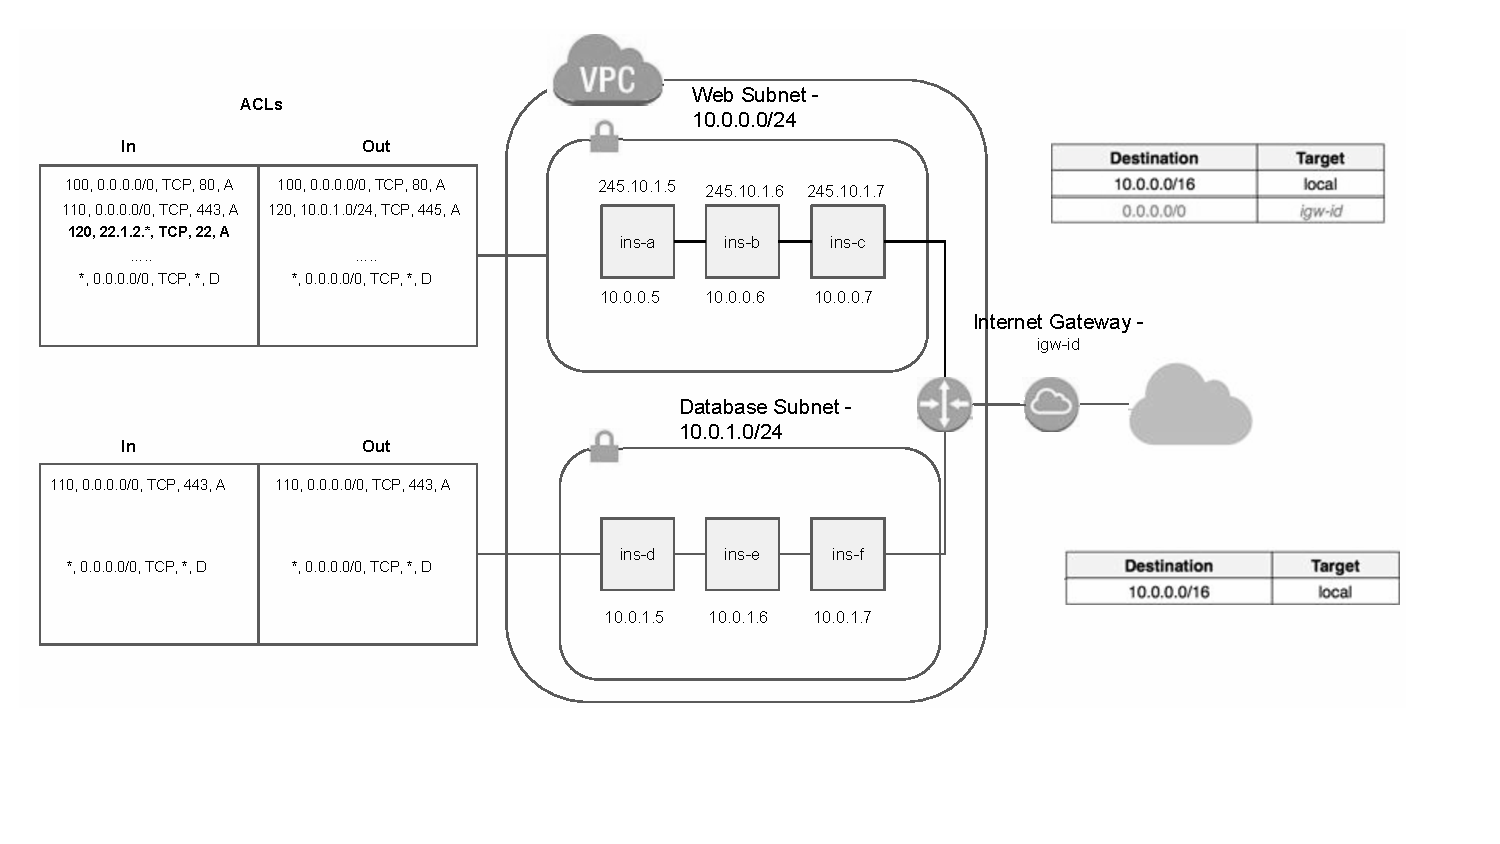
\includegraphics[width=1.0\textwidth]{./aws/fig/vpc2.pdf}
\caption{An example of a VPC network.\label{fig:aws/vpc}}
\end{figure}

This network consists of an internet gateway, two subnets ``Web'' and ``Database'' and three network nodes in each of them. Each of the subnets is assigned with a route table (on the right) and an access control list (ACL, on the left). The route tables allow the network traffic to flow between the subnets and between the ``Web'' subnet and the internet gateway. In other words, the network nodes in the ``Web'' subnet are accessible from the internet, while the nodes in the ``Database'' subnet are not. An ACL consists of rules that filter the network traffic to and from its subnet. In our example, one of the ACL rules of the ``Database'' subnet forbids SSH access to its nodes, both directly and through an intermediate node.

Imagine that this network grows over time and has more nodes and security and access rules added to it. A network administrator may want to make sure that the network retains certain properties after each change in its configuration. For example, the network administrator may want to check the following property.
\begin{example}\label{prop:bool-property}
All network nodes in the subnet ``Web'' can access all network nodes in the subnet ``Database''.
\end{example}

The network administrator might also want to know which networking components satisfy a given property, such as the ones described in the following example.
\begin{example}\label{prop:list-property}
All network nodes that have the port 22 (SSH) accessible from the internet.
\end{example}

We will refer to questions that network administrators might want to answer, such as the ones in Examples~\ref{prop:bool-property} and \ref{prop:list-property}, as \emph{network questions}. In particular, we will refer to questions similar to Example~\ref{prop:bool-property} as \emph{yes-no questions}, because an answer to them is ``yes'' or ``no'', and to questions similar to Example~\ref{prop:list-property} as \emph{list questions}, because an answer to them is a list of networking components. Each yes-no question can be equivalently phrased as a list question such that the answer to the yes-no question is ``yes'' iff the answer to the correspondent list questions is not empty. However, we distinguish these two types of questions because, as we show later, we can more efficiently answer them using different techniques.

Answering network questions manually might be tedious and error-prone in an industrial-size network. For this reason it is necessary to automate this task with specialised tools. In this work we employ automated reasoning tools for first-order logic. To this end, we build static models of VPC networks (Section~\ref{sect:aws/specification}), translate these models and network questions about them to problems in first-order logic (Section~\ref{sect:aws/fol}) and check these problems using finite model builders and saturation-based theorem provers (Section~\ref{sect:aws/fol-provers}). In Section~\ref{sect:aws/fol-provers} we argue that for our purposes these two types of reasoning tools complement each other: finite model builders can more efficiently answer list questions and saturation-based theorem provers can more efficiently answer yes-no questions. In Section~\ref{sect:aws/related} we cite related work and in Section~\ref{sect:aws/challenges} we describe the challenges that we faced in this work and outline future work.

%-------------------------------------------------------------------------------
\section{Network Reachability Properties}
\label{sect:aws/specification}
We answer network questions by building a static model of the network and reasoning about properties of this model. Our \emph{network model} consists of two parts, the \emph{formal specification} and the \emph{snapshot} of the network. The specification formalises the semantics of each of the components available in the network. For example, the formal specification describes how a route table directs network traffic in a subnet or in which order a firewall applies rules in an access control list. The snapshot describes the topology of the given network. For example, the snapshot contains the list of network nodes, subnets and their route tables. Naturally, the formal specification in the model of each particular VPC network is the same, whereas the snapshot differs. We used models of Amazon VPC networks as part of our ongoing work on network verification using complementary constraint solvers. We express network questions in the language of many-sorted first-order logic. In this section we describe syntax and semantics of network models and network questions.

\subsection{Network Models}
\label{sect:aws/reachability/spec}
A network model is a finite set of first-order Horn clauses expressed in a logic programming style. We disallow function symbols with positive arity and allow stratified negation. We assume the plain logic programming semantics for these Horn clauses, defined in the standard way (see e.g.~\cite{DBLP:books/sp/Lloyd87}). In particular, we make the closed-world assumption and treat negation as failure. In addition, our network models use equality and the theory of bit vectors to describe ports, port ranges, IPv4 addresses and subnet masks.

A \emph{signature} of the network model is a triple $(T, C, P),$ where $T$ is a set of \emph{types}, $C$ is a set of \emph{constants} and $P$ is a set of \emph{predicates}. We assign each constant with a type $\tau\in T$ and each predicate with a type $\tau_1\times\ldots\times\tau_n$ $(n\ge0)$, where $\tau_i\in T$ for each $1\leq i \leq n$. We assume a countable infinite set of \emph{variables}. We assign each variable with a type $\tau\in T$. We call a \emph{term} of the type $\tau\in T$ a constant or a variable of that type. We call an \emph{atom} an expression of the form $p(t_1,\ldots,t_n)$, where $n>0$, $p\in P$ is a predicate of the type $\tau_1\times\ldots\times\tau_n$ and each $t_i$, $1\leq i \leq n$ is a term of the type $\tau_i$. We call a \emph{literal} an atom or its negation.

A \emph{rule} is a Horn clause of the form $A\leftarrow L_1 \wedge \ldots \wedge L_n$ $(n \ge 0)$, where the \emph{head} of the rule $A$ is an atom and each of $L_1,\ldots,L_n$ is a literal. If $n=0$ and all arguments of $A$ are constants then we call such rule a fact. We call a \emph{definition} of the predicate $p \in P$ the set of all rules in the network model that use $p$ in their head.

The specification part of the model contains types, constants, predicates and rules that describe the semantics of the networking components used in the network. For example, the specification defines the semantics of SSH tunneling. One network node can SSH tunnel to another node iff it can either connect to it over SSH directly, or through a chain of one or more intermediate nodes. In order to express this concept, the specification contains predicates $\pred{canSshTunnel}$ and $\pred{canSsh}$, each of the type $\type{node}\times\type{node}$, and the two following rules.
\begin{align*}
\pred{canSshTunnel}(\mathit{Node}_1,\mathit{Node}_2)\leftarrow\:&\pred{canSsh}(\mathit{Node}_1,\mathit{Node}_2). \\
\pred{canSshTunnel}(\mathit{Node}_1,\mathit{Node}_2)\leftarrow\:&\pred{canSshTunnel}(\mathit{Node}_1,\mathit{Node}_3)\\
\wedge\:&\pred{canSshTunnel}(\mathit{Node}_3,\mathit{Node}_2).
\end{align*}
% can-ssh-tunnel-enis: eni * eni
% -: can-ssh-tunnel-enis Eni1 Eni2
% <- can-ssh-enis Eni1 Eni2.
% -: can-ssh-tunnel-enis Eni1 Eni2
% <- can-ssh-tunnel-enis Eni1 Eni3
% <- can-ssh-tunnel-enis Eni3 Eni2.

The snapshot part of the model contains constants and facts that describe the configuration of the networking components in a given network. For example, the snapshot of a network with a single node \verb'i-abcd1234' in a single subnet ``Web'' consists of the constants $\const{node}_\text{abcd1234}$ and $\const{subnet}_\text{Web}$, and the fact $\pred{nodeHasSubnet}(\const{node}_\text{abcd1234},\const{subnet}_\text{Web}).$

We assume that the signature contains
\begin{enumerate*}[label=(\roman*)]
  \item types $\type{bits16}$ and $\type{bits32}$;
  \item $2^{16}$ constants of the type $\type{bits16}$;
  \item $2^{32}$ constants of the type $\type{bits32}$;
  \item predicates $\pred{bits16}_{\le}$ and $\pred{bits16}_{\ge}$ of the type $\type{bits16} \times \type{bits16}$ with a special semantics; and
  \item predicate $\pred{bits32}_\wedge$ or the type $\type{bits32}\times\type{bits32}\times\type{bits32}$ with a special semantics.
\end{enumerate*}
$\type{bits16}$ and $\type{bits32}$ represent the types of 16-bit and 32-bit vectors. The semantics of the predicates is that of the correspondent operations over bit vectors defined in the standard way.

The network specification uses 16-bit vectors to encode port numbers (as integers between 0 and 65535) and port ranges, and 32-bit vectors to encode IPv4 addresses and subnet masks. Port ranges are represented using the type $\type{portRange}$ and the predicate $\pred{portRange}$ of the type $\type{portRange}\times\type{bits16}\times\type{bits16}$. For example, the port range 0--1023 is represented as the constant $\const{portRange}_\text{0--1023}$ of the type $\type{portRange}$ and the fact $\pred{portRange}(\const{portRange}_\text{0--1023},\allowbreak\const{bits16}_0,\allowbreak\const{bits16}_{1023})$, where $\const{bits16}_0$ and $\const{bits16}_{1023}$ are constants of the type $\type{bits16}$. The network specification contains the following definition of the predicate $\pred{portRangeOverlap}$ of the type $\type{portRange}\times\type{portRange}$ that holds when two port ranges overlap.
\begin{equation*}
  \begin{aligned}
\pred{portRangeOverlap}(\mathit{Range}_1,\mathit{Range}_2)\leftarrow\:&\:\pred{portRange}(\mathit{Range}_1,\mathit{From}_1,\mathit{To}_1) \\
  \wedge\:&\:\pred{portRange}(\mathit{Range}_2,\mathit{From}_2,\mathit{To}_2) \\
  \wedge\:&\:\pred{bits16}_\le(\mathit{From}_1,\mathit{To}_2) \\
  \wedge\:&\:\pred{bits16}_\le(\mathit{From}_2,\mathit{To}_1).
  \end{aligned}
\end{equation*}

Finally, we assume that for each type $\tau\in T$ the signature contains the predicate $\pred{=}_\tau$ of the type $\tau\times\tau$ interpreted as equality.

The specification of Amazon~VPC networks that we used in this work consists of approximately 50 types, 200 predicates and over 240 rules.

% Mention how large network snapshots get?

\subsection{Network Questions}
\label{sect:aws/reachability/properties}

We express network questions as formulas of many-sorted first-order logic with the standard logical connectives $\vee$, $\wedge$, $\Rightarrow$, $\Leftrightarrow$, $\oplus$ and equality. These formulas only use types, constants and predicates from the signature of the network model. The formulas do not use any function symbols. We allow interpretation of these formulas to use empty domains and otherwise assume the standard semantics of many-sorted first-order logic.

We express yes-no questions as closed formulas, that is, formulas in which all variables are bound by a quantifier. Conversely, we express list questions as formulas with free variables. The answer to a yes-no question is ``yes'' iff its correspondent formula is valid. The answer to a list question is the set of substitutions of free variables with constants that satisfy its correspondent formula.

Formula~\ref{eq:bool-property} expresses the yes-no question in Example~\ref{prop:bool-property}.
\begin{equation}\label{eq:bool-property}
\begin{aligned}
&(\forall w:\type{node})(\forall d:\type{node})\\
&\quad(\pred{nodeHasSubnet}(w, \const{subnet}_\text{Web})\:\wedge\:\\
&\quad\,\,\,\pred{nodeHasSubnet}(d, \const{subnet}_\text{Database}) \Rightarrow~\\
&\quad\,\,\,\quad\pred{nodeCanConnectToNode}(w,d))
\end{aligned}
\end{equation}
% true: all W D: (atom/instance-subnet(W, subnet/web) &&
% atom/instance-subnet(D, subnet/database)) =>
% instance-can-connect-to-instance(W, D).
%In this formula predicates $\pred{instanceHasSubnet}$ and $\pred{instanceCanConnectToInstance}$, and constants $\const{subnet}_\text{Web}$ and $\const{subnet}_\text{Database}$ are part of the signature of the network model~--- the predicate are available in the specification, and the constants are available in the snapshot.

% We illustrate this difference with the following property.
% \[
% (\forall \mathit{eni}:\type{eni})(\pred{eniOk(\mathit{eni})\vee\neg\pred{eniOk}(\mathit{eni})})
% \]
% % all Eni: (eni-ok(Eni) || !eni-ok(Eni))
% If this query was a formula in first-order logic, it would be a tautology. However, we interpret the property as true iff there exists at least one ENI in the network, that is, if the $\type{eni}$ type is inhabited by at least one value.

Formula~\ref{eq:list-property} expresses the list question in Example~\ref{prop:list-property}. In this formula $n$ of the type $\type{node}$ is a free variables.
\begin{equation}\label{eq:list-property}
\begin{aligned}
\pred{reachablePublicTcpUdp}(&\const{dir}_\text{ingress}, \const{proto}_6, n, \const{port}_{22},\\
                             &\const{publicIp}_\text{8:8:8:8}, \const{port}_\text{40000})
\end{aligned}
\end{equation}
% list: instance-has-eni(Instance, Eni) &&
%         reachable-public-tcp-udp(dir/ingress, proto/6,
%                                          Eni, port/22,
%                                          public-ip/8-8-8-8, port/40000).

All predicates and constants used in Formulas~\ref{eq:bool-property} and \ref{eq:list-property} are part of the signature of the network model. Constants $\const{subnet}_\text{Web}$ and $\const{subnet}_\text{Database}$ are part of the network snapshot, and all other predicates and constants are part of the network specification.

% %-------------------------------------------------------------------------------
% \section{Checking Properties with \Datalog}
% \label{sect:aws/datalog}
% We answer a network question by translating the network model and the network question to a \Datalog program and then running it using the \Datalog engine \souffle\cite{souffle}. A \Datalog program consists of a \Datalog \emph{query} and a finite set of \Datalog \textit{rules}. We obtain a query from the network question and a set of rules from both the network model and the network question. We assume that each \Datalog rule has the standard form $A\rl L_1\comma\ldots\comma L_n$ $(n\ge0)$, where $A$ is an atom and each of $L_1,\ldots,L_n$ is a literal, and a \Datalog query has the form $L_1\comma\ldots\comma L_n$ $(n\ge0)$, where each of $L_1,\ldots,L_n$ is a literal. We also assume that all \Datalog rules use stratified negation.

% Network specification is intentional database, network snapshot is extensional database.

\souffle accepts definitions of typed relations, contains the predefined symbol and numeric types, and accepts definitions of new types. The types in \souffle are interpreted under the open-world assumption. We model the types of the network models, interpreted as finite domains, using \Datalog relations with one argument. Let $\tau$ be a type and $c_1,\ldots,c_n$ ($n\ge0$) be constants of this type. We introduce a relation $\typedRel{\tau}$ and add the facts $\typed{\tau}{c_i}$, $1\le i\le n$ to the set of \Datalog rules. We use literals of the form $\typed{\tau}{t}$ in every \Datalog rule to guard the argument $t$ of the type $\tau$ in the head of the rule. % Mention that we can simplify it and only use typing literals near negations.

Let $p(t_1,\ldots,t_n)\leftarrow L_1\wedge\ldots\wedge L_m$ $(n\ge0,m\ge0)$ be a rule in the network model, where $p$ is a predicate of the type $\tau_1\times\ldots\times\tau_n$ and each of $L_1,\ldots,L_m$ is a literal. We translate $p$ to a \Datalog relation $r$ and translate this rule to the \Datalog rule $$r(t_1,\ldots,t_n)\rl\typed{\tau_1}{t_1}\comma\ldots\comma\typed{\tau_n}{t_n}\comma L_1\comma\ldots\comma L_m.$$

We translate a network question expressed as a first-order formula $\phi$ without function symbols to a \Datalog query and a set of \Datalog rules. We start by converting $\phi$ to a prenex disjunctive normal form that is $$(\forall x_1:\tau_1)\ldots(\forall x_n:\tau_n)(\exists y_1:\sigma_1)\ldots(\exists y_m:\sigma_m)(C_1\vee\ldots\vee C_k),$$ where $n\ge0$, $m\ge0$, $k\ge0$, and each of $C_1,\ldots,C_k$ is a conjunction of literals. Let $z_1:\upsilon_1,\ldots,z_l:\upsilon_l$ be all free variables of $\phi$. $l=0$ for formulas expressing boolean network questions and $l>0$ for formulas expressing list network question. We introduce two fresh relations $r$ and $q$ of the types $\tau_1\times\ldots\times\tau_n\times\upsilon_1\times\ldots\times\upsilon_l$ and $\upsilon_1\times\ldots\times\upsilon_l$, respectively. The translated set of \Datalog rules consists of $k+1$ rules: $k$ rules of the form
\begin{align*}
r(x_1,\ldots,x_n,z_1,\ldots,z_l)\rl\;&\typed{\tau_1}{x_1}\comma\ldots\comma\typed{\tau_n}{x_n}\comma~\\
                                     &\typed{\upsilon_1}{z_1}\comma\ldots\comma\typed{\upsilon_l}{z_l}\comma C_i
\end{align*}
for each $1\le i\le k$ and the rule
\begin{align*}
q(z_1,\ldots,z_l)\rl\typed{\upsilon_1}{z_1}\comma\ldots\comma\typed{\upsilon_l}{z_l}\comma\neg r(x_1,\ldots,x_n,z_1,\ldots,z_l).
\end{align*}
Note that we can use each conjunction $C_i$ in a \Datalog rule because each literal in $C_i$ only contains variables and constants~--- there are no function symbols in $\phi$ and they do not appear during a conversion to prenex disjunctive normal form. Finally, the \Datalog query is $\neg q(z_1,\ldots,z_l)$.

% Explain why negations are needed.

We translate types $\type{bits16}$ and $\type{bits32}$ to numeric types for 32 and 16-bit integers, respectively, and translate the predicates over bit vectors into their correspondent built-in \souffle operations.

We illustrate our translation using examples from Section~\ref{sect:aws/motivation}. We translate Formula~\ref{eq:bool-property} that expresses a boolean network question to the \Datalog rules
\begin{align*}
r(W,D)\rl\;& \typed{instance}{W}\wedge\neg\pred{instanceHasSubnet}(W,\const{subnet}_\text{Web}).\\
r(W,D)\rl\;& \typed{instance}{D}\wedge\neg\pred{instanceHasSubnet}(D,\const{subnet}_\text{Database}).\\
r(W,D)\rl\;& \typed{instance}{W}\wedge\typed{instance}{D}\:\wedge\:\\
           & \pred{instanceCanConnectToInstance}(W,D).\\
q\rl\;& \neg r(W,D).
\end{align*}
and the \Datalog query $\neg q$. Note that multiple rules in the definition of $r$ appear because of the translation to disjunctive normal form. We translate Formula~\ref{eq:list-property} that expresses a list network question to the \Datalog rules
\begin{align*}
r(I,E)\rl\;& \typed{instance}{I}\wedge\typed{eni}{E}\:\wedge\:\\
           & \pred{instanceHasEni}(I,E)\:\wedge\:\\
           &\begin{aligned}
               \pred{reachablePublicTcpUdp}(&\const{dir}_\text{ingress},\const{proto}_6,E,\const{port}_{22},\\
                                            &\const{publicIp}_\text{8:8:8:8},\const{port}_\text{40000}).
             \end{aligned}\\
q(I,E)\rl\;& \typed{instance}{I}\wedge\typed{eni}{E}\wedge\neg r(I,E).
\end{align*}
and the \Datalog query $\neg q(I,E)$.

%For example, consider a list query expressed by the formula $(\forall x:\tau)(\exists y:\sigma)(r(x, y) \wedge g(y))$, where $r$ and $g$ are predicates in the network model. We translate it to a \Datalog relation $p$ of the type $\tau\times\sigma$ and a nullary \Datalog relation $q$, two \Datalog rules $p(X,Y)\rl r(X,Y)\comma g(Y)$ and $q\rl \neg p(X,Y)$, and a \Datalog query $\neg q$.


%-------------------------------------------------------------------------------
\section{Checking Properties with Theorem Provers}
\label{sect:aws/fol-provers}
% The continuous advances in automated reasoning have made theorem provers into powerful tools capable of efficiently solving problems coming from real world domains. %\EK{FMB might be just as efficient as datalog search, and saturation-based proof search might be more efficient.} 

We translate network models and network questions to problems in first-order logic. Some of these problems use theories. We solve these problems using saturation-based theorem provers and finite model builders. We use the combination of these two types of provers to leverage the strengths of both of them, which we summarize below.

Saturation-based theorem provers such as E~\cite{E13}, Spass~\cite{Spass} or Vampire~\cite{Vampire13} construct proofs of unsatisfiability of first-order problems. To that end, they first convert the input problem into a set of first-order clauses and then try to derive contradiction from it. Theorem provers saturate the search space by inferring new clauses with inference rules such as binary resolution~\cite{Ganzinger01} and superposition~\cite{NieuwenhuisRubio:HandbookAR:paramodulation:2001}. They employ multiple techniques to prune the search space such as simplification orderings, selection functions and redundancy elimination. Saturation-based provers handle theories by adding incomplete first-order theory axioms to the set of clauses and by using specialised inference rules. In addition to that, \vampire implements the AVATAR modulo theories~\cite{DBLP:conf/gcai/RegerB0V16} architecture that relies on an SMT solver for theory-consistent reasoning in the ground subset of the problem. Saturation-based provers are designed to efficiently solve unsatisfiable problems. Given a satisfiable problem, saturation-based provers can in rare cases report satisfiability and output the saturated set of clauses. However, it is usually not possible to reconstruct a model from this set.

Finite model builders (finders) construct finite counter-models of first-order problems. One of the most successful methods for finite model building was pioneered by the finite model builder MACE~\cite{mccune1994davis}. This method iterates over possible domain sizes, for each domain size grounds the first-order problem with this domain, and translates the resulting formula to a SAT problem. If the SAT problem is satisfied, a finite model of the selected size is reconstructed from the SAT model. Finite model builders Gandalf~\cite{Gandalf}, Paradox~\cite{claessen2003new} and Vampire~\cite{VampireFMB} implement the MACE-style method. Finite model builders generally do not support theories with the notable exception of SMT solver CVC4~\cite{CVC4} that integrates model finding techniques into theory reasoning~\cite{CVC4FMB}. Finite model builders are designed to efficiently solve satisfiable problems. Given an unsatisfiable problem, some finite model builders might detect that the problem cannot have infinite models and in such case report unsatisfiability.

We translate
\begin{enumerate*}[label=(\roman*)]
  \item each yes-no question to a first-order problem that is unsatisfiable iff the answer to the question is ``yes''; and
  \item each list question to a first-order problem such that each of its finite models corresponds to an answer to the network question.
\end{enumerate*}
Table~\ref{fig:fol-answering-questions} summarises how we interpret a solution found by a reasoning tool as the answer to the network question. Saturation-based theorem provers generally cannot answer list questions except for the degenerate case when the answer is empty. With this exception, both types of provers are able to answer both types of network questions. 

\begin{table}
  \center
  \begin{tabular}{lll}
    \hline
    Output of a reasoning tool & Yes-no question & List question \\
    \hline
    Saturation found unsat & yes & empty list \\
    Saturation found sat   & no  & error \\
    FMB found unsat        & yes & empty list \\
    FMB found a model      & no  & list of answers \\
  \end{tabular}
  \caption{Solutions found by saturation-based theorem provers and finite model builders (FMB) interpreted as answers to network questions.}
  \label{fig:fol-answering-questions}
\end{table}

%Informally speaking, finite model builders can efficiently answer list questions and saturation-based provers can efficiently answer yes-no questions. To complement the performance of a finite model builder and a saturation-based prover, we run both of them in parallel on each first-order problem and record the result of the fastest successful run.

We run a finite model builder and a saturation-based prover in parallel on each problem and record the result of the fastest successful run. We expect that in most cases
\begin{enumerate*}[label=(\roman*)]
  \item a yes-no question can be answered with ``yes'' by the saturation-based prover and with ``no'' by the finite model builder; and
  \item a list question can be answered with the empty list by the saturation-based prover and with a non-empty list by the finite model builder.
\end{enumerate*}

In this work we used the \vampire theorem prover both as a saturation-based theorem prover and a finite model builder. Our translation produces problems expressed in a logic supported by \vampire, namely many-sorted first-order logic with equality, extended with the theory of linear integer arithmetic, the theory of arrays~\cite{VampireAndFOOL} and the theory of tuples~\cite{KKV18}. We wrote the problems in the TPTP language~\cite{TPTP}.

Each problem tackled by a saturation-based theorem prover or a finite model builder consists of the first-order formula $\phi$ that expresses the network question and first-order axioms $A_1,\ldots,A_n$ that we translate from the network model. We translate each yes-no question to a problem of the form $A_1\wedge\ldots\wedge A_n \Rightarrow \neg\phi$ and each list question to a problem of the form $A_1\wedge\ldots\wedge A_n \wedge (\forall \bar{z})(q(\bar{z})\Leftrightarrow \phi) \Rightarrow (\forall \bar{z})q(\bar{z}),$ where $q$ is a fresh predicate symbol and $\bar{z}$ are fresh free variables of $\phi$. We reconstruct the answer to a list question from the model of the $q$ predicate~--- each substitution of $\bar{z}$ that satisfies $q$ is an answer to the question.

\section{Network Reachability as a First-Order Problem}\label{sect:aws/fol}
Our translation of network models to problems in first-order logic consists of translations of types, constants, predicate definitions and theories. We translate types, constants (Section~\ref{sect:aws/fol/types}) and predicate definitions (Section~\ref{sect:aws/fol/predicates}) using Clark completion~\cite{DBLP:conf/adbt/Clark77}. We use specialised translations for the theory of bit vectors (Section~\ref{sect:aws/fol/theories}) because Vampire does not support it.

\subsection{Types and Constants}\label{sect:aws/fol/types}
Let $\tau$ be a type and $c_1,\ldots,c_n$ ($n\ge0$) be constants of this type. If $n>0$ then we introduce a sort $\tau$, constants $c_1,\ldots,c_n$ of this sort, the domain closure axiom of the form $(\forall x:\tau)(x=c_1 \vee\ldots\vee x=c_n)$ and the distinct constants axiom of the form of a conjunction of literals $c_i\not=c_j$ for all $1\le i\le n$, $1\le j\le n$ and $i\not=j$. If $n=0$ then we do not introduce any sorts or constants and in our translation of predicate definitions replace each subformula of the form $(\forall x:\tau)\varphi$ with logical truth and each subformula of the form $(\exists x:\tau)\varphi$ with logical falsum.

For example, the signature contains the type $\type{dir}$ and two constants $\const{dir}_\text{ingress}$ and $\const{dir}_\text{egress}$ of this type. $\type{dir}$ represents the direction of a network package. We translate this type to first-order logic as a sort $\mathit{dir}$, two constants $\mathit{ingress}$ and $\mathit{egress}$ of this sort and axioms $(\forall x:\mathit{dir})(x=\mathit{ingress}\vee x=\mathit{egress})$ and $\mathit{ingress}\neq\mathit{egress}$.

% dir: type.
% dir/ingress: dir.
% dir/egress: dir.

\subsection{Predicate Definitions}\label{sect:aws/fol/predicates}
%The definitions of predicates in the specification assume the closed world interpretation. It means that a predicate is satisfied iff at least one of its rules is satisfied. To capture the definition in first-order logic we translate a predicate definition using logical equivalence.

Let predicate $p$ of the type $\tau_1\times\ldots\times\tau_n$ be defined using $k\ge0$ rules. Let $x_1:\tau_1,\ldots,x_n:\tau_n$ be fresh variables. If $k=0$ then we translate the definition of $p$ to the axiom $$(\forall x_1:\tau_1)\ldots(\forall x_n:\tau_n)(\neg p(x_1,\ldots,x_n)).$$ If $k>0$ then we translate the definition of $p$ to the axiom $$(\forall x_1:\tau_1)\ldots(\forall x_n:\tau_n)(p(x_1,\ldots,x_n)\Leftrightarrow R_1\vee\ldots\vee R_k),$$ where each of the formulas $R_1,\ldots,R_k$ are translations of each of the $k$ rules, respectively.

Let a rule be of the form $$p(t_1,\ldots,t_n)\leftarrow L_1\wedge\ldots\wedge L_m,\quad(m\ge0)$$ where $t_1:\tau_1,\ldots,t_n:\tau_n$ are terms. Let $y_1:\sigma_1,\ldots,y_l:\sigma_l$ be variables that occur in either of $L_1,\ldots,L_m$ but not in $p(t_1,\ldots,t_n)$. If $m=0$ then we translate the rule to the formula $x_1=t_1\wedge\ldots\wedge x_n=t_n.$ If $m>0$ then we translate the rule to the formula
\begin{equation*}
\begin{aligned}
&x_1=t_1\wedge\ldots\wedge x_n=t_n\;\wedge(\exists y_1:\sigma_1)\ldots(\exists y_l:\sigma_l)(L_1\wedge\ldots\wedge L_m).
\end{aligned}
\end{equation*}

%The translation of rules can be refined to only include equalities for non-distinct variables in the head of the rule. The details of such modification are straightforward.

For example, consider the following definition of the predicate $\pred{link}$ of the type $\type{node} \times \type{node}$ that encodes the equivalence relation between two $\type{node}$s. The definition of $\pred{link}$ in not present in the network model, but it is illustrative of our translation.
\begin{equation*}
\begin{aligned}
&\pred{link}(X,X).\\
&\pred{link}(X,Y)\leftarrow\pred{link}(Y,X).\\
&\pred{link}(X,Y)\leftarrow\pred{link}(X,Z)\wedge\pred{link}(Z,Y).
\end{aligned}
\end{equation*}
% link: node * node
% -: link X X.
% -: link X Y
% <- link Y X.
% -: link X Y
% <- link X Z
% <- link Z Y.

We translate the definition of $\pred{link}$ as a predicate symbol $\mathit{Link}: \mathit{node} \times \mathit{node}$ and the axiom
\begin{equation*}
\begin{aligned}
&(\forall x:\mathit{node})(\forall y:\mathit{node})\\
&\quad
 \begin{aligned}
  (\mathit{Link}(x,y)\Leftrightarrow\:&x=y\:\vee\:\\
                                      &Link(y,x)\:\vee\:\\
                                      &(\exists z:\mathit{node})(\mathit{Link}(x,z)\wedge\mathit{Link}(z,y))).
 \end{aligned}
\end{aligned}
\end{equation*}

We translate the equality predicate $\pred{=}_\tau$ for each type $\tau$ to the standard equality in first-order logic. %Our translation ignores (the lack of) definitions of bit vector predicates and instead uses other theories as described in the following section.

\subsection{Theories}
\label{sect:aws/fol/theories}
Our experiments with translating the theory of bit vectors revealed that the quality of this translation crucially affects the performance of Vampire. This led us to develop and compare multiple translations. In this section we first describe translations of bit vectors that use other theories supported by Vampire. Then, we describe a network model transformation that eliminates theories from network models by precomputing the results of theory operations. Finally, we compare these translations.

\subsubsection*{Translations to Other Theories}
Recall that our network models use
\begin{enumerate*}[label=(\roman*)]
  \item the type $\type{bits16}$ and predicates $\pred{bits16}_{\le}$ (``less or equal''), $\pred{bits16}_{\ge}$ (``greater or equal'') and $\pred{=}_\type{bits16}$, and
  \item the type $\type{bits32}$ and predicates $\pred{bits32}_\wedge$ (bitwise conjunction) and $\pred{=}_\type{bits32}$.
\end{enumerate*}
%These two theories use different predicates, therefore we translate 16-bit and 32-bit vectors differently.
We translate 16-bit vectors to integers and 32-bit vectors to arrays and tuples.

\paragraph{16-bit vectors to integers.}
We translate
\begin{enumerate*}[label=(\roman*)]
  \item the type $\type{bits16}$ to $\mathbb{Z}$,
  \item each of the 16-bit vector constants to an integer constant, and
  \item each of the 16-bit predicates to their correspondent predicate symbol in the theory of linear integer arithmetic.
  \item predicate $\pred{=}_\type{bits16}$ to the standard equality.
\end{enumerate*}

\paragraph{32-bit vectors to arrays.}
We translate
(i) the type $\type{bits32}$ to the array sort $\mathit{array}(\mathbb{Z},\mathit{bool})$,
(ii) each of the 32-bit vector constant to a fresh constant $v$ of this sort, defined using the axiom $\mathit{select}(v,1)=b_1\wedge\ldots\wedge\allowbreak\mathit{select}(v, 32)=b_{32},$ where each of $b_1,\ldots,b_{32}$ is either $\mathit{true}$ or $\mathit{false}$, and
(iii) predicate $\pred{bits32}_\wedge$ to a predicate defined by the axiom of bitwise conjunction for arrays of Booleans.
\begin{equation*}
\begin{aligned}
&(\forall x:\mathit{array}(\mathbb{Z},\mathit{bool}))(\forall y:\mathit{array}(\mathbb{Z},\mathit{bool}))(\forall z:\mathit{array}(\mathbb{Z},\mathit{bool}))\\
&\quad\begin{aligned}
      (\mathit{bits32}_\wedge(x,y,z)\liff\:&(\mathit{select}(z,1)\liff\mathit{select}(x,1)\wedge\mathit{select}(y,1))\:\wedge\\
      &\quad\ldots\\
      \wedge\:&(\mathit{select}(z,32)\liff\mathit{select}(x,32)\wedge\mathit{select}(y,32)))
      \end{aligned}
\end{aligned}
\end{equation*}
(iv) predicate $\pred{=}_\type{bits32}$ to a predicate defined by the following axiom of equality for 32-element arrays of Booleans.
\begin{equation*}
\begin{aligned}
&(\forall x:\mathit{array}(\mathbb{Z},\mathit{bool}))(\forall y:\mathit{array}(\mathbb{Z},\mathit{bool}))\\
&\quad\begin{aligned}
      (\pred{=}_\type{bits32}(x, y)\liff\:&\mathit{select}(x,1)=\mathit{select}(y,1)\:\wedge\\
      &\quad\ldots\\
      \wedge\:&\mathit{select}(x, 32)=\mathit{select}(y,32))
      \end{aligned}
\end{aligned}
\end{equation*}

\paragraph{32-bit vectors to tuples.}
We translate
(i) the type $\type{bits32}$ to the tuple sort $(\mathit{bool},\ldots,\mathit{bool})$ where $\mathit{bool}$ is repeated 32 times,
(ii) each of the 32-bit vector constants to a term $(b_1,\ldots,b_{32})$ of this sort, where each of $b_1,\ldots,b_{32}$ is either $\mathit{true}$ or $\mathit{false}$, and
(iii) predicate $\pred{bits32}_\wedge$ to a predicate defined by the following axiom of bitwise conjunction for Boolean tuples.
\begin{equation*}
\begin{aligned}
&(\forall x_1\ldots x_{32}:\bool)(\forall y_1\ldots y_{32}:\bool)(\forall z_1\ldots z_{32}:\bool)\\
&\quad(\mathit{bits32}_\wedge((x_1,\ldots,x_{32}),(y_1,\ldots,y_{32}),(z_1,\ldots,z_{32}))\liff\\
&\quad\quad (z_1\liff x_1\wedge y_1)\wedge\ldots\wedge(z_{32}\liff x_{32}\wedge y_{32}))
\end{aligned}
\end{equation*}
(iv) predicate $\pred{=}_\type{bits32}$ to the standard equality.

% \paragraph{Extra optimisation.}
% We discovered that operators over 32-bit vectors are only ever used in the following context:
% \begin{equation*}
% \begin{aligned}
% \pred{=}_{bits32}(&\pred{bits32}_{\wedge}(\mathit{CidrBase}_1,\mathit{CidrMask}), \\
%                   &\pred{bits32}_{\wedge}(\mathit{CidrBase}_2,\mathit{CidrMask}))
% \end{aligned}
% \end{equation*}

% Solution~-- fuse them together. Instead of translating equality and conjunction
% \begin{enumerate}
%   \item introduce a predicate $\mathit{EqMask}: \mathit{cidrBase}\times\mathit{cidrBase}\times\mathit{cidrMask}$;
%   \item translate each term of the form \texttt{bits/32/eq (bits/32/and x m) (bits/32/and y m)} into $\mathit{EqMask}(x, y, m)$, and
%   \item add an axiom for $\mathit{EqMask}$.
% \end{enumerate}

\subsubsection*{Precomputation of Theories}
Our network models use 16-bit vectors to describe port numbers and port ranges and 32-bit vectors to describe IPv4 addresses and subnet masks. Bit vector predicates are only used in the definitions of predicates for network primitives. For example, 16-bit vectors only occur in the definitions of predicates that encode set-theoretic operations over port ranges, such as $\pred{portRangeOverlap}$ mentioned in Section~\ref{sect:aws/reachability/properties}. Definitions of higher level predicates only use these operations over port ranges and never the bit vectors predicates.

We eliminate theory terms and literals from network models by rewriting the definitions of set-theoretic operations over network primitives with results of precomputation of these operations for all primitives used in the network. For example, we precompute the $\pred{portRangeOverlap}$ predicate in the following way. First, we compute the set $S$ of all pairs of overlapping port ranges among the ones used in the network. This requires a quadratic number of integer comparisons. Then, we use set $S$ to build a definition of $\pred{portRangeOverlap}$ that consists of facts of the form $\pred{portRangeOverlap}(\const{portRange}_X,\const{portRange}_Y)$ where $(X,Y)\in S$. We optimise precomputation of some operations by considering their algebraic properties. For example, $\pred{portRangeOverlap}$ is a reflexive symmetric binary relation and 0--65535 overlaps with any other port range. Therefore, we avoid comparing each port range with itself, comparing two port ranges twice and comparing 0--65535 with other port ranges. Instead, we use the following rules in the definition of $\pred{portRangeOverlap}$.
\begin{equation}\label{eq:aws/port-range-algebraic}
\begin{aligned}
&\pred{portRangeOverlap}(\mathit{Range},\mathit{Range}).\\
&\pred{portRangeOverlap}(\mathit{R}_1,\mathit{R}_2)\leftarrow\pred{portRangeOverlap}(\mathit{R}_2,\mathit{R}_1).\\
&\pred{portRangeOverlap}(\const{portRange}_\text{0--65535},\mathit{Range}).
\end{aligned}
\end{equation}

%Here we describe a transformation that eliminates types and predicates of the theory of bit vectors from a network model. The resulting network model can be translated to plain many-sorted first-order logic without theories.

%The motivation for this transformation lies in the following observation. Port numbers in the network models are represented as 16-bit vectors. While the type of 16-bit vectors describes a domain with $2^{16}$ elements, most networks only use a handful of port numbers anywhere in their configuration. We can drastically decrease the size of the domain

%Notice that many networks only use a limited number of CIDR addresses and ports. We found that we could improve performance by representing a CIDR as finite domain that consists only of CIDRs that are used in the network and pre-compute the results of all operations over CIDRs.

%Before translating the network model to first-order logic we remove the $\pred{portRange}$ predicate from the model and rewrite the definition of $\pred{portRangeOverlap}$ in the following way.

% \begin{equation*}
% \begin{aligned}
% &\pred{portRangeOverlap}(\const{portRange}_\text{0--65535},\const{portRange}_\text{0--65535}).\\
% &\pred{portRangeOverlap}(\const{portRange}_\text{0--65535},\const{portRange}_\text{443--443}).\\
% &\pred{portRangeOverlap}(\const{portRange}_\text{0--65535},\const{portRange}_\text{5432--5432}).\\
% &\pred{portRangeOverlap}(\const{portRange}_\text{0--65535},\const{portRange}_\text{80--81}).\\
% &\pred{portRangeOverlap}(\const{portRange}_\text{0--65535},\const{portRange}_\text{9000--9000}).\\
% &\pred{portRangeOverlap}(\const{portRange}_\text{22--22},\const{portRange}_\text{0--65535}).\\
% &\pred{portRangeOverlap}(\const{portRange}_\text{443--443},\const{portRange}_\text{0--65535}).\\
% &\pred{portRangeOverlap}(\const{portRange}_\text{5432--5432},\const{portRange}_\text{0--65535}).\\
% &\pred{portRangeOverlap}(\const{portRange}_\text{80--80},\const{portRange}_\text{0--65535}).\\
% &\pred{portRangeOverlap}(\const{portRange}_\text{80--81},\const{portRange}_\text{0--65535}).\\
% &\pred{portRangeOverlap}(\const{portRange}_\text{80--81},\const{portRange}_\text{80--80}).\\
% &\pred{portRangeOverlap}(\const{portRange}_\text{80--80},\const{portRange}_\text{80--81}).\\
% \end{aligned}
% \end{equation*}

Consider a network that only uses port ranges 0--65535, 22--22, 443--443, 5432--5432, 80--80 and 80--81 in any of the configurations of its components. We found that it is not uncommon for our networks to use trivial port ranges that span one port number. The definition of $\pred{portRangeOverlap}$ precomputed for this network consists of 12 facts or the rule $\pred{portRangeOverlap}(\const{portRange}_\text{80--80},\const{portRange}_\text{80--81})$ together with the rules (\ref{eq:aws/port-range-algebraic}).

The precomputation of theories is the only applicable strategy for translating network models for Vampire's finite model builder, because it only supports plain many-sorted first-order logic without theories.

\subsubsection*{Comparison of Translations}
To compare the translation methods, we used each of them to encode 10 network verification problems in first-order logic and run \vampire in the saturation mode on the resulting formulas. Our verification problems express the property (\ref{prop:bool-property}) of 10 VPC network configurations. These network configurations are variations of the example on Figure~\ref{fig:aws/vpc} with different number of network nodes in each of the subnets ``Web'' and ``Database'' (from 1 to 10).

Table~\ref{table:aws/results} presents the runtimes of Vampire on each of the problems. Dashes indicate the absence of a solution within the given time limit of 1 minute. These results were obtained on a MacBook Pro with a 2,9 GHz Intel Core i5 and 8 Gb RAM.

\begin{table}\center
  \caption{Runtimes in seconds of Vampire on the network verification problems translated using different methods.}
  \label{table:aws/results}
  \begin{tabular}[ht]{lrrrrr}
\hline
\multirow{2}{*}{Translation} & \multicolumn{5}{c}{Number of network nodes} \\
                             & \multicolumn{1}{c}{1} & \multicolumn{1}{c}{2} & \multicolumn{1}{c}{3} & \multicolumn{1}{c}{4} & \multicolumn{1}{c}{5} \\
\hline
Arrays         & ~0.67 & ~2.52 & ~7.86 & 43.19 &    -- \\
Tuples         & ~0.44 & ~1.34 & ~2.92 & ~5.79 & ~8.81 \\
Precomputation & ~0.23 & ~0.38 & ~1.06 & ~1.82 & ~3.70 \\
  \end{tabular}

%   \begin{tabular}[ht]{lrrrrrrrrrr}
% \hline
% \multirow{2}{*}{Translation} & \multicolumn{10}{c}{Number of network nodes in each subnet} \\
%                              & \multicolumn{1}{c}{1} & \multicolumn{1}{c}{2} & \multicolumn{1}{c}{3} & \multicolumn{1}{c}{4} & \multicolumn{1}{c}{5} & \multicolumn{1}{c}{6} & \multicolumn{1}{c}{7} & \multicolumn{1}{c}{8} & \multicolumn{1}{c}{9} & \multicolumn{1}{c}{10} \\
% \hline
% Arrays         & 0.67 & 2.52 & 7.86 & 43.19 & -- & -- & -- & -- & -- & -- \\
% Tuples         & 0.44 & 1.34 & 2.92 & 5.79 & 8.81 & 17.28 & -- & 27.29 & -- & -- \\
% Precomputation & 0.23 & 0.38 & 1.06 & 1.82 & 3.70 & 6.61 & 10.90 & 7.12 & 14.57 & 37.11 \\
%   \end{tabular}
\vspace{1em}
  \begin{tabular}[ht]{lrrrrr}
\hline
\multirow{2}{*}{Translation} & \multicolumn{5}{c}{Number of network nodes} \\
                             & \multicolumn{1}{c}{6} & \multicolumn{1}{c}{7} & \multicolumn{1}{c}{8} & \multicolumn{1}{c}{9} & \multicolumn{1}{c}{10} \\
\hline
Arrays         &    -- &    -- &    -- &    -- &    -- \\
Tuples         & 17.28 &    -- & 27.29 &    -- &    -- \\
Precomputation & ~6.61 & 10.90 & ~7.12 & 14.57 & 37.11 \\
  \end{tabular}
\end{table}

The results of this experiment show that on this collection of verification problems formulas produced by the translation of 32-bit vectors to tuples are easier for \vampire than formulas produced by the translation to arrays. We explain it by the fact that the former end up using a more compact representation of bit vectors in first-order logic. The translation to tuples models a 32-bit vector as a single term, while the translation to arrays models it as conjunction of 32 literals. Furthermore, the translation to tuples uses the standard equality that Vampire supports efficiently, while the translation to arrays uses a heavy equality axiom for 32-element arrays. The compact representation of bit vectors as tuples allows Vampire infer bitwise conjunctions faster.

We observe that formulas produced by the translation with precomputed theories are easier for \vampire than formulas produced by any of the translations of bit vectors to other theories. We explain it by the fact that the bulky axioms for bitwise conjunction and equality slow down the proof search, whereas these operations are easy to precompute. Although the precomputation of a theory operation has polynomial complexity, we found that for the networks we used in this study it does not significantly slow down answering network questions. Realistic VPC networks only use a small number of distinct network primitives such as port numbers and IP addresses in any of the configurations of its components and the precomputation for them is not heavy. Furthermore, the precomputation of each theory operation usually involves a simple operation over machine integers that can be performed quickly.

%Overall we found the precomputation of theories to be the most efficient strategy for translating our network models. It is also the only applicable strategy for translating network models for Vampire's finite model builder, because it only supports plain many-sorted first-order logic without theories. % As mentioned here, we do not build models for bit vectors. Even if we did, why would they be huge? If represented as tuples, each 32-bit vector would be just a single term with 32 Boolean arguments.

%-------------------------------------------------------------------------------
\section{Related Work}
\label{sect:aws/related}

Network verification is an attractive target for automated reasoning tools, some of which we mentioned earlier in Section~\ref{sect:aws/introduction}. In this section we focus on approaches to network verification that are most similar to this work and applications of finite model building and saturation theorem proving to similar problems.

Network analysis based on the modelling of network components and protocols in first-order logic has been described in \cite{Karl2006,Hirt2006}. Compared to our work, these works rely on finite saturation in the Spass theorem prover to build models, and not on finite model builders. Another significant difference is the encoding of port numbers and IP addresses in network models. The approach taken in \cite{Karl2006,Hirt2006} represents port numbers as uninterpreted constants and IP addresses as 32-bit vectors modelled as a 32-ary function symbols with a special term simplification ordering added to Spass. This approach limit scalability of network analysis, e.g. complex routing rules involving many port intervals result in bulky first-order formulas. In contrast, our work offers a more efficient representation of port numbers and IP addresses.

Bj\o{}rner et al.~\cite{DBLP:conf/icdcit/BjornerJ15} checked properties of ACLs, routing tables and Border Gateway Protocol policies in Microsoft Azure networks using SMT solver Z3~\cite{Z3}. To that end \cite{DBLP:conf/icdcit/BjornerJ15} implemented a translation of network properties to quantifier-free logical formulas over bit vectors that is aware of the semantics of network components. In comparison, our translation encodes the complete semantics of a VPC network in the quantified problem solved by saturation-based theorem prover and finite model builders. We argue that our approach is more flexible at the expense of having to deal with more difficult problems.

Weidenbach~\cite{Weidenbach99} verified security properties of the Neuman-Stubblebine key exchange protocol by expressing them as sets of monadic Horn clauses. Similarly to our work, \cite{Weidenbach99} expressed reachability as unsatisfiability in first-order logic and used a saturation-based theorem prover to construct proofs of reachability. Conversely, \cite{Weidenbach99} discovered unreachability by finite saturation in Spass. Goubault-Larrecq~\cite{DBLP:journals/jcs/Goubault-Larrecq10} used finite model building to check unreachability in the context of verification of security protocols.

% ConfigChecker~\cite{ConfigChecker}~--- verification of ACLs, BDD, CRL symbolic model checking, not SDN though.

%VeriFlow~\cite{Veriflow}~--- checking network-wide invariants in real time, specialised algorithm, verification in the data plane.

%Anteater~\cite{Anteater}~--- data plane verification using SAT.

%CrystalNet~\cite{crystalnet}: Emulation of Large Production Networks

%Synthesis of network configurations using \Datalog~\cite{DBLP:conf/cav/El-HassanyTVV17}.

%-------------------------------------------------------------------------------
\section{Challenges and Future Work}
\label{sect:aws/challenges}
This paper presents a work in progress and some of the challenges that we faced are yet to be overcome. We discuss these challenges in this section and suggest directions for future work. We believe that similar challenges are experienced in other practical applications of automated reasoning in first-order logic.

\paragraph{Good translation to first-order logic.}
Automated theorem provers for first-order logic are known to be sensitive to the encoding of the problem they are solving. To ensure efficient representation of practical problems in a theorem prover, these problems should be encoded using theories and syntactical constructs beyond plain first-order logic. Yet not all automated theorem provers efficiently implement these features. While the Vampire theorem prover used in this work supports many useful theories, we miss a support for the theory of bit vectors. The need to work around this limitation hinders a good translation of our network model to first-order logic. %The lack of support for bit vectors led us to device multiple translations for this theory and experiment with these translations.

% In addition, theorem provers differ in the extensions of plain first-order logic and theories that they support, so one has to target a logic supported by a specific prover when devising a translation.

\paragraph{Configuration of theorem provers.}
Automated theorem provers typically offer many settings for configuring proof search. For example, Vampire has dozens of options~\cite{DBLP:conf/cade/Reger0V14} that describe a colossal number of possible proof strategies. There is no proof strategy that would be the best for all kinds of problems, and we found that changing the default options of Vampire might result in a strategy that works better on our problems than the default strategy. At the same time, hand-picking good options is tedious and unintuitive, and there is no way of knowing if a hand-picked strategy will work well on all of our problems. Many modern automated theorem provers rely not on one single strategy, but on a portfolio of strategies, which they try one by one during proof search. Theorem provers typically implement portfolios for existing large collections of problems such as TPTP~\cite{TPTP} and SMT-LIB~\cite{SMT-LIB}. To our knowledge, there is no systematic way of assembling a custom portfolio tailored to a specific class of problems.

% \paragraph{Surprising runtime.}
% When comparing the performance of \Datalog and theorem provers we saw that the performance time of \Datalog grows accordingly to the complexity of the problem. Performance of theorem provers looks unpredictable due to the nature of the saturation-based proof search. It's cool when a seemingly hard problem has an easy solution, not so cool the other way around. We wonder if a theorem proving community has an answer to it.

\paragraph{Finite domains.}
Our formalisation of VPC networks uses large finite domains to describe the topology of a network and the semantics of its components. While finite domains is good news for finite model builders, saturation-based theorem provers are known to have hard time reasoning with them. Domain closure axioms $(\forall x:\tau)(x=c_1 \vee\ldots\vee x=c_n)$ for large values of $n$ result in long clauses that degrade performance of the prover. A technique for efficient superposition theorem proving with these axioms is discussed e.g. in \cite{HillenbrandWeidenbach13}, but this technique is not implemented in any modern theorem prover.

\paragraph{EPR.}
We translate network models to problems that almost fit into the effectively propositional (EPR) fragment of first-order logic, also called the Bernays-Sch\"onfinkel class. These problems do not use function symbols with positive arity, but Skolem functions with positive arity might be introduced during clausification. The satisfiability problem for EPR is decidable and there exist efficient tools that deal with this fragment~\cite{DBLP:conf/birthday/Korovin13}. It is possible to translate our network models to problems in EPR, for example by grounding the existentially-quantified variables. The obvious drawback of this translation is the blowup of the size of the resulting problem. Whether this blowup is mitigated by the efficiency of EPR solvers is an interesting question for future work.

\paragraph{Solver-agnostic network models.}
The work presented in this paper contributes to our ultimate goal of checking network properties with diverse complementary constraint solvers. In order to successfully use different kinds of constraint solvers we need a formalisation of networks that can be equally efficiently translated to different kinds of constraint satisfaction problems. We find that our current formalisation, written in the logic programming style, is friendly for systems like \Datalog~\cite{Datalog}, but not necessarily for theorem provers for first-order logic. For example, some of the predicates in the specification can be more naturally expressed as functions in full first-order logic rather than translated from their encoding as Horn clauses. Ultimately this bias hinders efficient representation of the problem in first-order logic. Designing a more solver-agnostic formalisation of networks is an important direction of future work.

\paragraph{Evaluation.} In this work we used a small collection of network configurations that we verified using Vampire run as a saturation-based theorem prover. We leave for future work experiments with (i) other theorem provers for first-order logic, (ii) other kinds of constraint solvers, (iii) different encodings of network problems as constraint satisfaction problems, and (iv) large collections of real world network configurations.

%-------------------------------------------------------------------------------
\section*{Acknowledgments}
\label{sect:aws/acks}
This work has been partially carried out during the first author's visit to Amazon Web Services. We thank Koen Claessen for his valuable comments on an earlier draft of this paper. The first author was partially supported by the Wallenberg Academy Fellowship 2014 and the Swedish VR grant D0497701.


\def\paperFiveContentsTitle{TFX: The TPTP Extended Typed First-Order Form}
\def\paperFiveChapterTitle{TFX: The TPTP Extended Typed\\First-Order Form}
\def\paperFiveAuthors{Geoff~Sutcliffe and Evgenii~Kotelnikov}
\def\paperFiveAbstract{The TPTP world is a well established infrastructure that supports research, development, and deployment of Automated Theorem Proving systems for classical logics. The TPTP language is one of the keys to the success of the TPTP world. Originally the TPTP world supported only first-order clause normal form (CNF). Over the years support for full first-order form (FOF), monomorphic typed first-order form (TF0), rank-1 polymorphic typed first-order form (TF1), monomorphic typed higher-order form (TH0), and rank-1 polymorphic typed higher-order form (TH1), have been added. TF0 and TF1 together form the TFF language family; TH0 and TH1 together form the THF language family. This paper introduces the eXtended Typed First-order form (TFX), which extends TFF to include boolean terms, tuples, conditional expressions, and let expressions.}
\def\paperFivePublication{Published in the \emph{Proceedings of the 6th Workshop on Practical Aspects of Automated Reasoning}, pages 72--87. CEUR Workshop Proceedings, 2018.}
\paperchapter{\paperFiveContentsTitle}
             {\paperFiveChapterTitle}
             {\paperFiveAuthors}
             {\paperFiveAbstract}
             {\paperFivePublication}
\label{chap:tfx}
% !TEX root = ../main.tex

%------------------------------------------------------------------------------
\section{Introduction}
\label{sec:tfx/Introduction}

The TPTP world \cite{Sut10} is a well established infrastructure that supports
research, development, and deployment of Automated Theorem Proving (ATP)
systems for classical logics.
The TPTP world includes the TPTP problem library,
% \cite{Sut09}, 
the TSTP solution library,
% \cite{Sut10}, 
% the TMTP model library,
% \cite{SS16},
standards for writing ATP problems and reporting ATP solutions,
% \cite{SS+06,Sut08-KEAPPA}, 
tools and services for processing ATP problems and solutions,
% \cite{Sut10}, 
and it supports the CADE ATP System Competition (CASC).
% \cite{Sut16}.
Various parts of the TPTP world have been deployed in a range of applications,
in both academia and industry.
The web page \url{http://www.tptp.org} provides access to all components.

The TPTP language is one of the keys to the success of the TPTP world.
The language is used for writing both TPTP problems and TSTP solutions,
which enables convenient communication between different systems and
researchers.
Originally the TPTP world supported only first-order clause normal form (CNF)
\cite{SS98-JAR}.
Over the years support for full first-order form (FOF) \cite{Sut09},
monomorphic typed first-order form (TF0) \cite{tff0}, rank-1 polymorphic
typed first-order form (TF1) \cite{tff1}, monomorphic typed higher-order 
form (TH0) \cite{THF}, and rank-1 polymorphic typed higher-order form (TH1) 
\cite{KSR16}, have been added.
TF0 and TF1 together form the TFF language family; TH0 and TH1 together form 
the THF language family.
See \cite{Sut17} for a recent review of the TPTP.

Since the inception of TFF there have been some features that have 
received little use, and hence little attention. 
In particular, tuples, conditional expressions (\ITE), and let 
expressions (\LETIN) were neglected, and the latter two were horribly 
formulated with variants to distinguish between their use as formulae and 
terms. 
Recently, conditional expressions and let expressions have become more 
important because of their use in software verification applications.
In an independent development, Evgenii Kotelnikov et al. introduced FOOL
\cite{FOOL}, a variant of many-sorted first-order logic (FOL).
FOOL extends FOL in that it (i)~contains an interpreted boolean type, which
allows boolean variables to be used as formulae, and allows all formulae to be 
used as boolean terms, (ii)~contains conditional expressions, and 
(iii)~contains let expressions.
FOOL can be straightforwardly extended with the polymorphic theory of tuples 
that defines first class tuple types and terms \cite{KKV18}.
Features of FOOL can be used to concisely express problems coming from program
analysis~\cite{KKV18} or translated from more expressive logics. 
The conditional expressions and let expressions of FOOL resemble those of the 
SMT-LIB language version 2~\cite{SMT-LIB}.

The TPTP's new eXtended Typed First-order form (TFX) language remedies the
old weaknesses of TFF, and incorporates the features of FOOL.
This has been achieved by conflating (with some exceptions) formulae and 
terms, removing tuples from plain TFF, including fully expressive tuples in 
TFX, removing the old conditional expressions and let expressions from 
TFF, and including new elegant forms of conditional expressions and let 
expressions as part of TFX. 
(These more elegant forms have been mirrored in THF, but that is not a topic of
this paper.)
TFX is a superset of the revised TFF language. 
This paper describes the extensions to the TFF language form that define the 
TFX language.
The remainder of this paper is organised as follows:
Section~\ref{sec:tfx/TPTPFOOL} reviews the TFF language, and describes FOOL.
Section~\ref{sec:tfx/TFX} provides technical and syntax details of the new features 
of TFX.
Section~\ref{sec:tfx/ImplementationExamples} describes the evolving software 
support for TFX, and provides some examples that illustrate its use.
Section~\ref{sec:tfx/Conclusion} concludes.

%------------------------------------------------------------------------------
\section{The TFF Language and FOOL}
\label{sec:tfx/TPTPFOOL}

The TPTP language is a human-readable, easily machine-parsable, flexible and
extensible language, suitable for writing both ATP problems and solutions.
The top level building blocks of the TPTP language are {\em annotated 
formulae}.
An annotated formula has the form $$\mathit{language}\text{\tt(}\mathit{name}\text{\tt, }\mathit{role}\text{\tt, }\mathit{formula}\text{\tt, [}\mathit{source}\text{\tt, [}\mathit{useful\_info}\text{\tt]]).}$$
The {\em language}s supported are clause normal form (\lstinline'cnf'),
first-order form (\lstinline'fof'), typed first-order form (\lstinline'tff'), and
typed higher-order form (\lstinline'thf').
The {\em role}, e.g., \lstinline'axiom', \lstinline'lemma', \lstinline'conjecture',
defines the use of the formula in an ATP system.
In the {\em formula}, terms and atoms follow Prolog conventions, i.e.,
functions and predicates start with a lowercase letter or are {\tt '}single
quoted{\tt '}, variables start with an uppercase letter, and all
contain only alphanumeric characters and underscore.
The TPTP language also supports interpreted symbols, which either start with a
\lstinline'$', or are composed of non-alphanumeric characters, e.g., the truth
constants \lstinline'$true' and \lstinline'$false', and integer/rational/real
numbers such as \lstinline'27', \lstinline'43/92', \lstinline'-99.66'.
The basic logical connectives are
\lstinline'!', \lstinline'?', \lstinline'~', \lstinline'|', \lstinline'&', \lstinline'=>', \lstinline'<=',
\lstinline'<=>', and \lstinline'<~>',
for
$\forall$, $\exists$, $\neg$, $\vee$, $\wedge$, $\Rightarrow$, $\Leftarrow$,
$\Leftrightarrow$, and $\oplus$ respectively.
Equality and inequality are expressed as the infix operators \lstinline'=' and
\lstinline'!='.
The following is an example of an annotated first-order formula, supplied from a file.
\begin{lstlisting}[language=tptp]
fof(union, axiom,
    ![X, A, B]: (member(X, union(A, B)) <=>
      (member(X, A) | member(X, B))),
    file('SET006+0.ax', union),
    [description('Definition of union'), relevance(0.9)]).
\end{lstlisting}

%------------------------------------------------------------------------------
\subsection{The Typed First-Order Form TFF}
\label{sec:tfx/TFF}

TFF extends the basic FOF language with {\em types} and {\em type
declarations}.
The TF0 variant is monomorphic, and the TF1 variant is rank-1 polymorphic.
Every function and predicate symbol is declared before its use, with
a {\em type signature} that specifies the types of the symbol's arguments
and result. Each TF0 type is one of
\begin{itemize}
\item the predefined types \lstinline'$i' for $\iota$ (individuals) and
      \lstinline'$o' for $o$ (booleans);
\item the predefined arithmetic types \lstinline'$int' (integers), \lstinline'$rat'
      (rationals), and \lstinline'$real' (reals); or
\item user-defined types (constants).
\end{itemize}

User-defined types are declared before their use to be of the kind
\lstinline'$tType', in annotated formulae with the \lstinline'type' role~--- see
Figure~\ref{fig:tfx/TF0Example} for examples.
% All symbols share the same namespace; in particular, a type cannot have the
% same name as a function or predicate symbol.
Each TF0 type signature declares either
\begin{itemize}
\item an individual type $\tau$; or
\item a function type {\tt ($\tau_1\;$*$\;{\cdots}\;$*$\;\tau_n$)$\;$>$\;\tilde \tau$}
      for $n > 0$, where $\tau_i$ are the argument types, and $\tilde \tau$
      is the result type.
      % Argument types and the result type for a function cannot be
      % {\tt \$o}, and the result type for a predicate must be {\tt \$o}.
      % If $n = 1$ the parentheses are omitted.
\end{itemize}

The type signatures of uninterpreted symbols are declared like types, in
annotated formulae with the \lstinline'type' role~--- see Figure~\ref{fig:tfx/TF0Example}
for examples.
The type of \lstinline'=' and \lstinline'!=' is ad hoc polymorphic over all types 
except \lstinline'$o' (this restriction is lifted in TFX), with both arguments 
having the same type and the result type being \lstinline'$o'.
The types of arithmetic predicates and functions are ad hoc polymorphic
over the arithmetic types; see \cite{tff0} for details.
Figure~\ref{fig:tfx/TF0Example} illustrates some TF0 formulae, whose conjecture can
be proved from the axioms (it is the TPTP problem {\tt PUZ130\_1.p}).

\begin{figure}[htbp]
\begin{lstlisting}[language=tptp]
tff(animal_type, type, animal: $tType).
tff(cat_type, type, cat: $tType).
tff(dog_type, type, dog: $tType).
tff(human_type, type, human: $tType).
tff(cat_to_animal_type, type, cat_to_animal: cat > animal).
tff(dog_to_animal_type, type, dog_to_animal: dog > animal).
tff(garfield_type, type, garfield: cat).
tff(odie_type, type, odie: dog).
tff(jon_type, type, jon: human).
tff(owner_of_type, type, owner_of: animal > human).
tff(chased_type, type, chased: (dog * cat) > $o).
tff(hates_type, type, hates: (human * human) > $o).

tff(human_owner, axiom,
    ![A: animal]: ?[H: human]: H = owner_of(A)).

tff(jon_owns_garfield, axiom,
    jon = owner_of(cat_to_animal(garfield))).

tff(jon_owns_odie, axiom,
    jon = owner_of(dog_to_animal(odie))).

tff(jon_owns_only, axiom,
    ![A: animal]:
      (jon = owner_of(A)
     => (A = cat_to_animal(garfield)
       | A = dog_to_animal(odie)))).

tff(dog_chase_cat, axiom,
    ![C: cat, D: dog]:
      (chased(D, C)
     => hates(owner_of(cat_to_animal(C)),
              owner_of(dog_to_animal(D))))).

tff(odie_chased_garfield, axiom, chased(odie, garfield)).

tff(jon_hates_jon, conjecture, hates(jon, jon)).
\end{lstlisting}
\caption{TF0 Formulae.}
\label{fig:tfx/TF0Example}
\end{figure}

The polymorphic TF1 extends TF0 with (user-defined) {\em type constructors}, 
{\em type variables}, polymorphic symbols, and one new binder.
Each TF1 type is one of
\begin{itemize}
\item the predefined types \lstinline'$i' and \lstinline'$o';
\item the predefined arithmetic types \lstinline'$int', \lstinline'$rat', and 
      \lstinline'$real';
\item user-defined $n$-ary type constructors applied to $n$ type arguments; or
\item type variables, which must be quantified by \lstinline'!>' --- see the type
      signature forms below.
\end{itemize}

Type constructors are declared before their use to be of the kind
{\tt (\$tType$\;$*$\;{\cdots}\;$*$\;$\$tType)$\;$> \$tType}, in annotated 
formulae with a \lstinline'type' role.
Each TF1 type signature declares either
\begin{itemize}
\item an individual type $\tau$;
\item a function type {\tt ($\tau_1\;$*$\;{\cdots}\;$*$\;\tau_n$)$\;$>$\;\tilde \tau$}
      for $n > 0$, where $\tau_i$ are the argument types and $\tilde \tau$
      is the result type (with the same caveats as for TF0); or
\item a polymorphic type {\tt !>[$\alpha_1$:$\;$\$tType,$\;{\dots}\;$,$\alpha_n$:$\;$\$tType]:$\;\varsigma$}
      for $n > 0$, where $\alpha_1,\dots,\alpha_n$ are distinct
      type variables and $\varsigma$ is a TF0 type signature.
\end{itemize}

The \lstinline'!>' binder in the last form denotes universal quantification in the
style of $\lambda\Pi$ calculi.
It is used only at the top level in polymorphic type signatures.
All type variables must be of kind \lstinline'$tType'; more complex type variables
% e.g., {\tt \$tType$\;$>$\;$\$tType} 
are beyond rank-1 polymorphism.
An example of TF1 formulae can be found in \cite{KSR16}.

%------------------------------------------------------------------------------
\subsection{FOOL}
\label{sec:tfx/FOOL}

FOOL \cite{FOOL}, standing for First-Order Logic (FOL) + bOoleans, is a 
variant of many-sorted first-order logic. 
FOOL extends FOL in that it (i)~contains an interpreted boolean type, which
allows boolean variables to be used as formulae, and allows all formulae to be 
used as boolean terms, (ii)~contains conditional expressions, and 
(iii)~contains let expressions.
FOOL can be straightforwardly extended with the polymorphic theory of tuples 
that defines first class tuple types and terms \cite{KKV18}.
In what follows we consider such extension, and tuples are part of TFX.
There is a model-preserving transformation of FOOL formulae to FOL formulae
\cite{FOOL} that can be implemented in a FOL ATP system to support reasoning with FOOL.
Formulae of FOOL can also be efficiently translated to a first-order clausal 
normal form~\cite{FOOLCNF}. 
The following describes these features of FOOL, illustrating them using 
examples taken from \cite{VampireAndFOOL} and \cite{KKV18}.
The complete formal semantics of FOOL is given in~\cite{FOOL}.

%------------------------------------------------------------------------------
\subsubsection{Boolean Terms and Formulae}

FOOL contains an interpreted two-element boolean type $\bool$, allows 
quantification over variables of type $\bool$, and considers formulae to 
be terms of type $\bool$.
This allows boolean variables to be used as formulae, and all formulae to be 
used as boolean terms.
For example, Formula~\ref{eq:tfx/fool-bool-var} is a syntactically correct 
tautology in FOOL.
\begin{equation}\label{eq:tfx/fool-bool-var}
(\forall x:\bool)(x \lor \neg x)
\end{equation}
Logical implication can be defined as a binary function
$\mathit{imply}$ of the type $\bool \times \bool \to \bool$ using the axiom
\begin{equation}\label{eq:tfx/fool-imply}
(\forall x:\bool)(\forall y:\bool)(\mathit{imply}(x,y) \liff \neg x \lor y).
\end{equation}
Then it is possible to express that $P$ is a graph of a (partial) function of 
the type $\sigma \to \tau$ as
\begin{equation}\label{eq:tfx/bool-arg-example}
(\forall x:\sigma)(\forall y:\tau)(\forall z:\tau)
\mathit{imply}(P(x,y) \land P(x,z), y \eql z)
\end{equation}
Formula \ref{eq:tfx/fool-imply} can be equivalently expressed with $\eql$ instead of
$\liff$.

\subsubsection{Tuples}
FOOL extended with the theory of tuples contains a type
$\tuple{\sigma_1,\ldots,\sigma_n}$ of the $n$-ary tuple for all types
$\sigma_1,\ldots,\sigma_n$, $n>0$. Each type
$\tuple{\sigma_1,\ldots,\sigma_n}$ is first class, that is, it can be
used in the type of a function or predicate symbol, and in a quantifier. 
An expression $\tuple{t_1,\ldots,t_n}$, where $t_1,\ldots,t_n$ are
terms of types $\sigma_1,\ldots,\sigma_n$, respectively, is a tuple term of 
type $\tuple{\sigma_1,\ldots,\sigma_n}$. 
Each tuple term is first class and can be used as an argument to a function 
symbol, a predicate symbol, or equality.

Tuples are ubiquitous in mathematics and programming languages. For example,
one can use the tuple sort $\tuple{\mathds{R},\mathds{R}}$ as the sort of
complex numbers. 
Thus the term $\tuple{2,3}$ represents the complex number $2+3i$. 
A function symbol $\mathit{plus}$ that represents addition of complex numbers 
has the type $\tuple{\mathds{R},\mathds{R}} \times 
\tuple{\mathds{R},\mathds{R}} \to \tuple{\mathds{R},\mathds{R}}$.

\subsubsection{Conditional Expressions}
FOOL contains conditional expressions of the form $\ite{\psi}{s}{t}$, where 
$\psi$ is a formula, and $s$ and $t$ are terms of the same type. 
The semantics of such expressions mirrors the semantics of conditional 
expressions in programming languages, and they are therefore convenient for 
expressing formulae coming from program analysis. 
For example, consider the $\mathit{max}$ function of the type 
$\mathds{Z}\times\mathds{Z}\to\mathds{Z}$ that returns the maximum of its 
arguments. 
Its definition can be expressed in FOOL as
\begin{equation}\label{eq:tfx/ite-t-example}
(\forall x:\mathds{Z})(\forall y:\mathds{Z})
(\mathit{max}(x, y) \eql \ite{x \geq y}{x}{y}).
\end{equation}

FOOL allows conditional expressions to occur as formulae, as in the
following valid property of $\mathit{max}$.
\begin{equation}\label{eq:tfx/ite-f-example}
(\forall x:\mathds{Z})(\forall y:\mathds{Z})
(\ite{\mathit{max}(x, y) \eql x}{x \geq y}{y \geq x})
\end{equation}

\subsubsection{Let Expressions}
FOOL contains let expressions of the form $\letindef{D_1;\ldots;D_k}{t}$, where
$k > 0$, $t$ is either a term or a formula, and $D_1,\ldots,D_k$ are
simultaneous non-recursive definitions. FOOL allows definitions of function
symbols, predicate symbols, and tuples.

The definition of a function symbol 
$f:\sigma_1\times\ldots\times\sigma_n\to\tau$ has the form 
$\binding{f(x_1:\sigma_1,\ldots,x_n:\sigma_n)}{s}$, where
$n \geq 0$, $x_1,\ldots,x_n$ are distinct variables, and $s$ is a term of the type $\tau$.
For example, the following let expression denotes the maximum of three 
integer constants $a$, $b$, and $c$, using a local definition of the function 
symbol $\mathit{max}$.
\begin{equation}\label{eq:tfx/fool-let-imply}
\begin{aligned}
\mathtt{let}\;&\binding{\mathit{max}(x:\mathds{Z},y:\mathds{Z})}
                       {\ite{x \geq y}{x}{y}}\\
 \mathtt{in}\;&\mathit{max}(\mathit{max}(a,b),c)
\end{aligned}
\end{equation}

The definition of a predicate symbol $p:\sigma_1\times\ldots\times\sigma_n$ has 
the form $\binding{p(x_1:\sigma_1,\ldots,x_n:\sigma_n)}{\phi}$, where 
$n \geq 0$, $x_1,\ldots,x_n$ are distinct variables, and $\phi$ is a formula.
For example, the following let expression denotes equivalence of two boolean 
constants $A$ and $B$, using a local definition of the predicate symbol 
$\mathit{imply}$.
\begin{equation}\label{eq:tfx/fool-let-imply2}
\begin{aligned}
\mathtt{let}\;&\binding{\mathit{imply}(x:\bool,y:\bool)}{\neg x \lor y}\\
 \mathtt{in}\;&\mathit{imply}(A,B)\wedge\mathit{imply}(B,A)
\end{aligned}
\end{equation}

The definition of a tuple has the form $\binding{(c_1,\ldots,c_n)}{s}$, where
$n > 1$, $c_1,\ldots,c_n$ are distinct constant symbols of the types
$\sigma_1,\ldots,\sigma_n$, respectively, and $s$ is a term of the type
$(\sigma_1,\ldots,\sigma_n)$. 
For example, the following formula defines addition for complex numbers using 
two simultaneous local definition of tuples.
\begin{equation}\label{eq:tfx/fool-tuple-let}
  \begin{aligned}
  &(\forall x:(\mathds{R},\mathds{R}))(\forall y:(\mathds{R},\mathds{R}))\\
  &\quad(\mathit{plus}(x,y)\eql\letinpar{(a,b)}{x}{(c,d)}{y}{\tuple{a+c,b+d})}
  \end{aligned}
\end{equation}

The semantics of let expressions in FOOL mirrors the semantics of
simultaneous non-recursive local definitions in programming languages. 
That is, none of the definitions $D_1,\ldots,\allowbreak D_n$ uses function or
predicate symbols created by any other definition. 
In the following example, constants $a$ and $b$ are swapped by a let 
expression. 
The resulting formula is equivalent to $P(b, a)$.
\begin{equation}\label{eq:tfx/parallel-let-example}
\mathtt{let}\;\binding{a}{b}\,;\,\binding{b}{a}\;\mathtt{in}\;P(a, b)
\end{equation}

Formula~\ref{eq:tfx/parallel-let-example} can be equivalently expressed using 
the following let expression with a definition of a tuple.
\begin{equation}\label{eq:tfx/parallel-let-tuple-example}
\mathtt{let}\;\binding{(a,b)}{(b,a)}\;\mathtt{in}\;P(a, b)
\end{equation}

Let expressions with tuple definitions are convenient for expressing 
problems coming from program analysis, namely modelling of assignments
\cite{KKV18}.
The left hand side of Figure~\ref{fig:tfx/simple-if} shows an example of an 
imperative \texttt{if} statement containing assignments to integer variables, 
and an \texttt{assert} statement. 
This can be encoded in FOOL as shown on the right hand side, using 
let expressions with definitions of tuples that capture the assignments.

\begin{figure}[htbp]
\begin{center}
\begin{tabular}[t]{ll}
\begin{minipage}{0.26\textwidth}
\vspace{0.8cm}
\begin{lstlisting}[language=cpp]
if (x > y) {
   t := x;
   x := y;
   y := t;
}
assert(x <= y);
\end{lstlisting}
\end{minipage}
&\hspace{0.4cm}
\begin{minipage}{0.5\textwidth}
\[
  \letnl{(x,y,t)}{\itenll{x > y}
                 {\letinnl{t}{x}
                          {\letinnl{x}{y}
                                   {\letinnl{y}{t}
                                            {(x,y,t)}}}}
                 {(x,y,t)}}
        {x \le y}
\]
\end{minipage}
\\
\end{tabular}
\end{center}
\caption{FOOL encoding of an {\tt if} statement.}
\label{fig:tfx/simple-if}
\end{figure}

%------------------------------------------------------------------------------
\section{The TFX Syntax}
\label{sec:tfx/TFX}

The TPTP TFF syntax has been extended to provide the features of FOOL,
and at the same time some of the previous weaknesses have been remedied.
Formulae and terms have been conflated (with some exceptions).
Tuples have been removed from TFF, and fully expressive tuples included in 
TFX. 
The old conditional expressions and let expressions have been removed from 
TFF, and new elegant forms have been included as part of TFX. 
The grammar of TFX is captured in version v7.1.0.2 of the TPTP syntax,
available online at \url{http://www.tptp.org/TPTP/SyntaxBNF.html}.
In the subsections below, the relevant excerpts of the BNF are provided,
with examples and commentary.

%------------------------------------------------------------------------------
\subsection{Boolean Terms and Formulae}

Variables of type \lstinline'$o' can be used as formulae, and formulae can be 
used as terms. 
The following is the relevant BNF excerpt.
Formulae are terms are conflated by including logic/atomic formulae as
options for terms/unitary terms.
The distinction between formulae and terms is maintained for plain TFF.
\begin{lstlisting}[language=bnf]
<tff_logic_formula> ::=
    <tff_unitary_formula> | <tff_unary_formula>
  | <tff_binary_formula>  | <tff_defined_infix>
<tff_unitary_formula> ::=
    <tff_quantified_formula> | <tff_atomic_formula>
  | <tfx_unitary_formula>    | (<tff_logic_formula>)
<tfx_unitary_formula> ::= <variable>
<tff_term> ::=
    <tff_logic_formula> | <defined_term> | <tfx_tuple>
<tff_unitary_term> ::=
    <tff_atomic_formula> | <defined_term> | <tfx_tuple>
  | <variable> | (<tff_logic_formula>)
\end{lstlisting}

The FOOL tautology on Formula~\ref{eq:tfx/fool-bool-var} can be written in TFX as
\begin{lstlisting}[language=tptp]
tff(tautology, conjecture, ![X: $o]: (X | ~X)).
\end{lstlisting}

The $\mathit{imply}$ predicate in Formula~\ref{eq:tfx/fool-imply} can 
be written in TFX as
\begin{lstlisting}[language=tptp]
tff(imply_type, type, imply: ($o * $o) > $o).
tff(imply_defn, axiom,
    ![X: $o, Y: $o]: (imply(X, Y) <=> (~X | Y))).
\end{lstlisting}

% No longer necessary
% Notice that the negation of a boolean variable used as a formula must be
% placed inside parenthesis.

The definition of a graph of a function on Formula~\ref{eq:tfx/bool-arg-example} can be written in TFX as
\begin{lstlisting}[language=tptp]
tff(s, type, s: $tType).
tff(t, type, t: $tType).
tff(p, type, p: (s * t) > $o).
tff(graph, axiom,
    ![X: s, Y: t, Z: s]: imply(p(X, Y) & p(X, Z), Y = Z)).
\end{lstlisting}

A consequence of allowing formulae as terms is that the default typing of 
functions and predicates supported in plain TFF (functions default to 
{\tt (\$i * \ldots * \$i) > \$i} and predicates default to 
{\tt (\$i * \ldots * \$i) > \$o)} is not supported in TFX.

Note that not all terms can be used as formulae.
Tuples, numbers, and ``distinct objects'' cannot be used as formulae.

%------------------------------------------------------------------------------
\subsection{Tuples}

Tuples in TFX are written in {\tt []} brackets, and can contain any type of 
term, including formulae and variables of type \lstinline'$o'. 
Signatures can contain tuple types. 
The following is the relevant BNF excerpt.
\begin{lstlisting}[language=bnf]
<tfx_tuple_type> ::= [<tff_type_list>]
<tff_type_list> ::=
    <tff_top_level_type>
  | <tff_top_level_type>,<tff_type_list>
<tfx_tuple> ::= [] | [<tff_arguments>]
<tff_arguments> ::= <tff_term> | <tff_term>,<tff_arguments>
\end{lstlisting}

The tuple type $\tuple{\mathds{R},\mathds{R}}$ can be written in TFX 
as \lstinline|[$real, $real]| and the type of the addition function for 
complex numbers $\tuple{\mathds{R},\mathds{R}} \times 
\tuple{\mathds{R},\mathds{R}} \to \tuple{\mathds{R},\mathds{R}}$ can be 
written as \begin{center}\lstinline'([$real, $real] * [$real, $real]) > [$real, $real]'.\end{center}
The tuple term $\tuple{2,3}$ can be written as \lstinline'[2,3]'.
Tuples can occur only as terms, anywhere they are well-typed (i.e., they
cannot appear as formulae). In the following example the predicate \lstinline|p|
takes a tuple $(\mathds{Z},\iota,o)$ as the first argument.
\begin{lstlisting}[language=tptp]
tff(p_type, type, p: ([$int, $i, $o] * $o * $int) > $o).
tff(q_type, type, q: ($int * $i) > $o).
tff(me_type, type, me: $i).
tff(tuples_1, axiom,
    ![X: $int]: p([33, me, $true], ![Y: $i]: q(X, Y), 27)).
\end{lstlisting}

Note that while product types and tuple types are semantically equivalent,
two separate syntaxes are used to make it easy to distinguish 
between the following cases.
\begin{lstlisting}[language=tptp]
tff(n_type, type, n: [$int, $int]).
tff(f_type, type, f: [$int, $int] > $int).
tff(g_type, type, g: ($int * $int) > $int).
tff(h_type, type, h: ([$int, $int] * $int) > $int).
\end{lstlisting}

The first case defines \lstinline|n| to be a tuple of two integers.
The second case defines \lstinline|f| to be a function from a tuple of two integers
to an integer.
The third case defines \lstinline|g| to be a function from two integers to an integer.
The last case defines \lstinline|h| to be a function from a tuple of two integers and
an integer, to an integer.

The tuples syntax cannot be used to simultaneously declare types of multiple constants in an annotated formula with the \lstinline'type' role. For example, the following expression is not valid.
\begin{lstlisting}[language=tptp]
tff(ab_type, type, [a, b]: [$int, $int]).
\end{lstlisting}
Instead, one must declare the type of each constant separately.
\begin{lstlisting}[language=tptp]
tff(a_type, type, a: $int).
tff(b_type, type, b: $int).
\end{lstlisting}

%------------------------------------------------------------------------------
\subsection{Conditional Expressions}

Conditional expressions are polymorphic, taking a formula as the first 
argument, then two formulae or terms of the same type as the second and 
third arguments. 
The type of the conditional expression is the type of its second and third 
arguments. 
The following is the relevant BNF excerpt.
\begin{lstlisting}[language=bnf]
<tfx_conditional> ::= $ite(<tff_logic_formula>,
                           <tff_term>,<tff_term>)
\end{lstlisting}

The keyword \lstinline'$ite' is used for conditional expressions occurring both as
terms and formulae, which is different from the old TFF syntax of \ITE\ that
contained two separate keywords \lstinline'$ite_t' and \lstinline'$ite_f'.

The definition and a property of the $\mathit{max}$ function on Formulae~\ref{eq:tfx/ite-t-example} and \ref{eq:tfx/ite-f-example} can be expressed in
TFX as
\begin{lstlisting}[language=tptp]
tff(max_type, type, max: ($int * $int) > $int).
tff(max_defn, axiom,
    ![X: $int, Y: $int]:
      max(X, Y) = $ite($greatereq(X, Y), X, Y)).
tff(max_property, conjecture,
    ![X: $int, Y: $int]: 
      $ite(max(X, Y) = X, $greatereq(X, Y),
                          $greatereq(Y, X))).
\end{lstlisting}

%------------------------------------------------------------------------------
\subsection{Let Expressions}

Let expressions in TFX contain (i) the type signatures of locally defined 
symbols; (ii) the definitions of the symbols; and (iii) the term or formula
in which the definitions are used. 
Type signatures in let expressions syntactically match those in annotated 
formulae with the \lstinline'type' role. 
The symbol definitions determine how locally defined symbols are expanded 
in the term or formulae where they are used.
The type signature must include the types for all the local defined symbols.
The following is the relevant BNF excerpt.
\begin{lstlisting}[language=bnf]
<tfx_let> ::=
    $let(<tfx_let_types>,<tfx_let_defns>,<tff_term>)
<tfx_let_types> ::=
    <tff_atom_typing> | [<tff_atom_typing_list>]
<tff_atom_typing_list> ::=
    <tff_atom_typing>
  | <tff_atom_typing>,<tff_atom_typing_list>
<tfx_let_defns> ::= <tfx_let_defn> | [<tfx_let_defn_list>]
<tfx_let_defn> ::= <tfx_let_LHS> <assignment> <tff_term>
<tfx_let_LHS> ::= <tff_plain_atomic> | <tfx_tuple>
<tfx_let_defn_list> ::=
    <tfx_let_defn>
  | <tfx_let_defn>,<tfx_let_defn_list>
\end{lstlisting}

The keyword \lstinline'$let' is used for let expressions defining both function and 
predicate symbols, regardless of whether the let expression occurs as a term 
or a formula. 
This is different from the old TFF syntax of let expressions that contained 
four separate keywords \lstinline'$let_tt', \lstinline'$let_tf', \lstinline'$let_ft', and 
\lstinline'$let_ff'.

In the following example an integer constant \lstinline'c' is defined in a let expression.
\begin{lstlisting}[language=tptp]
tff(p_type, type, p: ($int * $int) > $o).
tff(let_1, axiom, $let(c: $int, c:= $sum(2, 3), p(c, c))).
\end{lstlisting}

The left hand side of a definition may contain pairwise distinct variables 
as top-level arguments, which can also appear in the right hand side
of the definition.
Such variables are implicitly universally quantified, and of the type 
defined by the symbol's type declaration.
The variables' values are supplied by unification in the defined symbol's use.
Figures~\ref{fig:tfx/let-tfx} and \ref{fig:tfx/let-tfx2} show examples of let expressions with definitions of function and predicate symbols.

\begin{figure}[htbp]
\begin{lstlisting}[language=tptp]
tff(max_max, axiom,
    $let(max: ($real * $real) > $real,
         max(X, Y) := $ite($greatereq(X, Y), X, Y),
         max(max(a, b), c))).
\end{lstlisting}
\caption{TFX encoding of Formula~\ref{eq:tfx/fool-let-imply}.}
\label{fig:tfx/let-tfx}
\end{figure}

\begin{figure}[htbp]
\begin{lstlisting}[language=tptp]
tff(a, type, a: $o).
tff(b, type, b: $o).
tff(a_eq_b, axiom,
    $let(imply: ($o * $o) > $o,
         imply(X, Y) := ~X | Y,
         imply(a, b) & imply(b, a))).
\end{lstlisting}
\caption{TFX encoding of Formula~\ref{eq:tfx/fool-let-imply2}.}
\label{fig:tfx/let-tfx2}
\end{figure}


Let expression can use definitions of tuples. 
Formula~\ref{eq:tfx/fool-tuple-let} can be written in TFX as follows. 
Notice that the type declaration contains the elements of both tuples in 
the simultaneous definition.
\begin{lstlisting}[language=tptp]
tff(plus, type,
    plus: ([$real, $real] * [$real, $real]) > [$real, $real]).
tff(plus_def, axiom,
    ![X: [$real, $real], Y: [$real$, $real]]:
      (plus(X, Y) 
      = $let([a: $real, b: $real, c: $real, d: $real],
             [[a, b] := X, [c, d] := Y],
             [$sum(a, c), $sum(b, d)])).
\end{lstlisting}

Sequential let expressions (\verb'let*') can be implemented by nesting. 
In the following example \lstinline'ff' and \lstinline'gg' are defined in sequence, and the let expression is equivalent to the formula \lstinline'p(f(i,i,i,i))'.
\begin{lstlisting}[language=tptp]
tff(i_type, type, i: $int).
tff(f_type, type, f: ($int * $int * $int * $int) > $int).
tff(p_type, type, p: $int > $o).
tff(let_tuple_3, axiom,
    $let(ff: ($int * $int) > $int,
         ff(X, Y):= f(X, X, Y, Y),
         $let(gg: $int > $int,
              gg(Z) := ff(Z, Z),
              p(gg(i))))).
\end{lstlisting}

Let expressions can have simultaneous local definitions
with the type declarations and the definitions given in {\tt []}es
(they look like tuples of declarations and definitions, but are
specified independently of tuples in the syntax).
(Lisp-like programming languages call them \verb'let', and 
not \verb'let*' --- \verb'let*' can be implemented in TFX by nesting
\verb'let's).
The symbols must have distinct signatures.
Figure~\ref{fig:tfx/pba-tfx} shows two equivalent let expressions, one with a tuple definition, the other with two simultaneous definitions of constants.
\begin{figure}[htbp]
\hspace{-0.24cm}
\begin{tabular}[t]{ll}
\begin{minipage}{0.48\textwidth}
\begin{lstlisting}[language=tptp]
tff(a, type, a: $i).
tff(b, type, b: $i).
tff(p, type, p: ($i*$i)>$o).
tff(pba, axiom,
    $let([a: $i, b: $i],
         [a := b, b := a],
         p(a, b))).
\end{lstlisting}
\end{minipage}
    &
\begin{minipage}{0.48\textwidth}
\begin{lstlisting}[language=tptp]
tff(a, type, a: $i).
tff(b, type, b: $i).
tff(p, type, p: ($i*$i)>$o).
tff(pba, axiom,
    $let([a: $i, b: $i],
         [a, b] := [b, a],
         p(a, b))).
\end{lstlisting}
\end{minipage}
\end{tabular}
\caption{TFX encodings of Formulas~\ref{eq:tfx/parallel-let-example} (left) and \ref{eq:tfx/parallel-let-tuple-example} (right).}
\label{fig:tfx/pba-tfx}
\end{figure}

In the following example two function symbols are defined simultaneously, and the let expression is equivalent to the formula \begin{center}\lstinline[language=tptp,backgroundcolor=\color{lstgrey}]{p(f(i,i,f(i,i,i,i),f(i,i,i,i)))}.\end{center}
\begin{lstlisting}[language=tptp]
tff(i_type, type, i: $int).
tff(f_type, type, f: ($int * $int * $int * $int) > $int).
tff(p_type, type, p: $int > $o).
tff(let_tuple_2, axiom,
    $let([ff: ($int * $int) > $int, gg: $int > $int],
         [ff(X, Y) := f(X,X,Y,Y), gg(Z) := f(Z,Z,Z,Z)],
         p(ff(i, gg(i))))).
\end{lstlisting}

The defined symbols of a let expression have scope over the formula/term in 
which the definitions are applied, shadowing any definition outside the let 
expression. 
The right hand side of a definition can have symbols with the same name as 
the defined symbol, but refer to symbols defined outside the let expression. 
In the following example the local definition of the \lstinline'array' function 
symbols shadow the global declaration.
\begin{lstlisting}[language=tptp]
tff(array_type, type, array: $int > $real).
tff(p_type, type, p: $real > $o).
tff(let_3, axiom,
    $let(array: $int > $real,
         array(I) := $ite(I = 3, 5.2, array(I)),
         p($sum(array(2), array(3))))).
\end{lstlisting}

% In this formula,
% \begin{itemize}
% \item \verb'array' occuring in the annotated formula with the \verb'type' role declares the type of a function globally;
% \item \verb'array' occurring on the left hand side of \verb':=' defines a function globally;
% \item \verb'array' occurring on the right hand side of \verb':=' refers to the globally declared function; and
% \item \verb'array' occurring in the third argument of the let expression refers to the locally defined function.
% \end{itemize}

%------------------------------------------------------------------------------
\section{Software Support and Examples}
\label{sec:tfx/ImplementationExamples}

%------------------------------------------------------------------------------
\subsection{Software for TFX}
\label{sec:tfx/Software}
The BNF provides the automatically generated lex/yacc parsers for TPTP files.
At the time of writing this paper, the TPTP4X utility is being upgraded
to support TFX.

The Vampire theorem prover \cite{Vampire13} supports all features of FOOL. 
Vampire transforms FOOL formulae into a set of first-order clauses using the 
VCNF algorithm \cite{FOOLCNF}, and then reasons with these clauses using 
its usual resolution calculi for first-order logic. 
At the time of writing this paper the latest released version of Vampire,
4.2.2, uses a syntax for FOOL that slightly differs from TFX. 
Full support for the TFX syntax has been implemented in a recent revision of 
the Vampire source code\footnote{%
\url{https://github.com/vprover/vampire}}, and will be available
in the next release of Vampire.

TFX has been used by two program verification tools BLT~\cite{CF-iFM17} and
Voogie~\cite{KKV18}. 
Both BLT and Voogie read programs written in a subset of the Boogie 
intermediate verification language and generate their partial correctness 
properties written in the TFX syntax. 
BLT and Voogie generate formulae differently, but both rely on features of 
FOOL, namely conditional expressions, let expressions, and tuples.

%------------------------------------------------------------------------------
\subsection{Examples}
\label{sec:tfx/Examples}

Figures~\ref{fig:tfx/TupleConditionalLet}--\ref{fig:tfx/Truthteller} show longer examples of
useful applications of features of FOOL. 
Figure~\ref{fig:tfx/TupleConditionalLet} shows how tuples, conditional expressions, 
and let expressions can be mixed, here to place two integer values in 
descending order as arguments in an atom. 
Figure~\ref{fig:tfx/LetITE} shows the TFX encoding of the FOOL formula in 
Figure~\ref{fig:tfx/simple-if}, which expresses a partial correctness property 
of an imperative program with an \texttt{if} statement. 
Figure~\ref{fig:tfx/Truthteller} shows an example that uses formulae as terms, in 
the second arguments of the \lstinline'says' predicate. 
The problem is to find a model from which it is possible to determine which 
of \lstinline'a', \lstinline'b', or \lstinline'c' is the only truthteller on this Smullyanesque 
island~\cite{Smu78}. 
More TFX examples are available from the TPTP web site 
\url{http://www.tptp.org/TPTP/Proposals/TFXExamples.tgz}.

\begin{figure}[ht]
\begin{lstlisting}[language=tptp]
tff(v1_type, type, v1: $int).
tff(v2_type, type, v2: $int).
tff(ordered_p, axiom,
    $let([large: $int,small: $int],
         [large, small] := $ite($greater(v1,v2),
                                [v1, v2], [v2, v1]),
         p(large, small))).
\end{lstlisting}
\caption{Mixing tuples, conditional and let expressions.}
\label{fig:tfx/TupleConditionalLet}
\end{figure}

\begin{figure}[ht]
\begin{lstlisting}[language=tptp]
tff(x, type, x: $int).
tff(y, type, y: $int).
tff(t, type, t: $int).
tff(x_leq_y, conjecture,
    $let([x: $int, y: $int, t: $int],
         [x, y, t] := $ite($greater(x,y),
                           $let(t: $int, t := x,
                           $let(x: $int, x := y,
                           $let(y: $int, y := t,
                                [x, y, t]))),
                           [x, y, t]),
         $lesseq(x, y))).
\end{lstlisting}
\caption{A TFX encoding of the program analysis problem in
Figure~\ref{fig:tfx/simple-if}.}
\label{fig:tfx/LetITE}
\end{figure}

\begin{figure}[ht]
\begin{lstlisting}[language=tptp]
tff(a_type, type, a: $i).
tff(b_type, type, b: $i).
tff(c_type, type, c: $i).
tff(exactly_one_truthteller_type, type,
    exactly_one_truthteller: $o).
tff(says, type, says: ($i * $o) > $o).

% Each person is either a truthteller or a liar
tff(island, axiom,
    ![P: $i]: (says(P, $true) <~> says(P, $false))).
tff(exactly_one_truthteller, axiom,
    (exactly_one_truthteller
  <=> (?[P: $i]: says(P,$true)
      & ![P1: $i, P2: $i]:
          ((says(P1, $true) & says(P2, $true))
         => P1 = P2)))).

% B said that A said that there is
% exactly one truthteller on the island
tff(b_says, hypothesis,
    says(b, says(a, exactly_one_truthteller))).

% C said that what B said is false
tff(c_says, hypothesis, says(c, says(b, $false))).
\end{lstlisting}
\caption{Who is the truthteller?}
\label{fig:tfx/Truthteller}
\end{figure}

%------------------------------------------------------------------------------
\section{Conclusion}
\label{sec:tfx/Conclusion}

This paper has introduced the eXtended Typed First-order form (TFX) of the
TPTP's TFF language.
TFX includes boolean variables as formulae, formulae as terms, tuple types and
terms, conditional expressions, and let expressions.
TFX is useful for (at least) concisely expressing problems coming from 
program analysis, and translated from more expressive logics.

Now that the syntax is settled, ATP system developers will be able to
implement the new language features.
It is already apparent from the SMT community that these are useful features,
and systems that can already parse and reason using the SMT version 2 language 
need only new parsers to implement the features of TFX.
In parallel, version v8.0.0 of the TPTP will include problems that use TFX,
and the automated reasoning community is invited to submit problems for
inclusion in TPTP.

\paragraph{Acknowledgements.}
Thanks to our friends in the TPTP World who have provided feedback on TFX
features, starting from the TPTP Tea Party at CADE-22 in 2009. The second
author was partially supported by the Wallenberg Academy Fellowship 2014 and
the Swedish VR grant D0497701.

\bibliography{refs}

\end{document}